%% ----------------------------------------------------------------
%% Thesis.tex -- MAIN FILE (the one that you compile with LaTeX)
%% ----------------------------------------------------------------

% Set up the document
\documentclass[a4paper, 11pt, oneside]{Thesis}  % Use the "Thesis" style, based on the ECS Thesis style by Steve Gunn
\graphicspath{figures/}  % Location of the graphics files (set up for graphics to be in PDF format)

\usepackage[T2A]{fontenc}
\usepackage[utf8]{inputenc}
\usepackage[english]{babel}

\usepackage{changepage}

\usepackage[table,xcdraw]{xcolor}

% Include any extra LaTeX packages required
\usepackage{natbib}  % Use the "Natbib" style for the references in the Bibliography
\setcitestyle{authoryear,round,citesep={;},aysep={,},yysep={;}}

\usepackage{bm}  % Allows "\bvec{}" and "\buvec{}" for "blackboard" style bold vectors in maths
\usepackage{xfrac}
\usepackage{tabularx}


\usepackage{hyperref}
\hypersetup{urlcolor=blue, colorlinks=true}  % Colours hyperlinks in blue, but this can be distracting if there are many links.

\newcommand{\fig}[1]{Figure~\ref{fig:#1}}
\newcommand{\sect}[1]{Section~\ref{sect:#1}}
\newcommand{\chapt}[1]{Chapter~\ref{chapt:#1}}
\newcommand{\tab}[1]{Table~\ref{tab:#1}}
\newcommand{\alg}[1]{Algorithm~\ref{alg:#1}}
\newcommand{\eq}[1]{(\eqref{eq:#1})}

\usepackage{todonotes}
% \usepackage{gensymb}
\usepackage{enumitem}

% Attempt to make hyperref and algorithmic work together better:
\newcommand{\theHalgorithm}{\arabic{algorithm}}
\usepackage{algorithm}
\usepackage{algpseudocode}
%\newcommand{\todo}[1][]{\@latex@warning{TODO #1}\fbox{TODO\dots}}


% \usepackage{bbm}
\usepackage{multirow}
\usepackage{subcaption}
\usepackage{graphicx}
\usepackage{mathtools}
% \usepackage{algorithmic}
% \usepackage{algorithmicx}
% \usepackage{algorithm2e}

% \usepackage{nomencl}
% \makenomenclature
% \setlength\nomlabelwidth{3.2cm}


% \renewcommand{\nomname}{List of Symbols and Abbreviations}
% \renewcommand{\nompreamble}{
%     Scalar numbers are denoted by unbolded letters ($x$),
%     bold $\mathbf{x}$ represents a vector and $x_i$ is an $i$-th element of the vector,
%     bold capital letter $\mathbf{X}$ represents a matrix,
%     while calligaphic capital $\mathcal{X}$ is typically used
%     to denote a tensor.
% }
% \usepackage{etoolbox}
% \renewcommand\nomgroup[1]{%
%   \item[
%   \ifstrequal{#1}{A}{\underline{Symbol}}{}%
% ]\underline{Meaning}}



\newcommand{\onot}{\mathcal{O}} % O-notation
\newcommand{\R}{\mathbb{R}}
\newcommand{\T}{\top}
\DeclareMathOperator*{\argmax}{arg\,max}
\DeclareMathOperator*{\argmin}{arg\,min}
\DeclareMathOperator{\cov}{cov}
\DeclarePairedDelimiter{\ceil}{\lceil}{\rceil}


\def\mystrut{\rule[-.3\baselineskip]{0pt}{0.5\baselineskip}}

\definecolor{inodefill}{HTML}{D9EAD3}
\definecolor{inodedraw}{HTML}{B6D7A8}
\definecolor{pnodefill}{HTML}{CFE2F3}
\definecolor{pnodedraw}{HTML}{9FC5E8}
\definecolor{onodefill}{HTML}{E6B8AF}
\definecolor{onodedraw}{HTML}{CC4125}
\definecolor{mnodefill}{HTML}{EAD1DC}
\definecolor{mnodedraw}{HTML}{D5A6BD}
\definecolor{goldfill}{HTML}{EAD7AC}
\definecolor{golddraw}{HTML}{D1AC71}
\definecolor{bluefill}{HTML}{5AB1F2}
\definecolor{bluedraw}{HTML}{0083E5}


%% ----------------------------------------------------------------
\begin{document}
\frontmatter      % Begin Roman style (i, ii, iii, iv...) page numbering

% Set up the Title Page
\title  {GAUSSIAN PROCESS MODELS FOR LARGE-SCALE PROBLEMS}
\authors  {\texorpdfstring
            {\href{y.kapushev@skoltech.ru}{Yermek Kapushev}}
            {Yermek Kapushev}
            }
\addresses  {\groupname\\\deptname\\\univname}  % Do not change this here, instead these must be set in the "Thesis.cls" file, please look through it instead
\date       {\today}
\subject    {}
\keywords   {}

\maketitle

%% ----------------------------------------------------------------

\setstretch{1.3}  % It is better to have smaller font and larger line spacing than the other way round

% Define the page headers using the FancyHdr package and set up for one-sided printing
\fancyhead{}  % Clears all page headers and footers
\rhead{\thepage}  % Sets the right side header to show the page number
\lhead{}  % Clears the left side page header

\pagestyle{fancy}  % Finally, use the "fancy" page style to implement the FancyHdr headers

%% ----------------------------------------------------------------
% Declaration Page required for the Thesis, your institution may give you a different text to place here
%\Declaration{

%\addtocontents{toc}{\vspace{1em}}  % Add a gap in the Contents, for aesthetics

%I, AUTHOR NAME, declare that this thesis titled, `THESIS TITLE' and the work presented in it are my own. I confirm that:

%\begin{itemize}
%\item[\tiny{$\blacksquare$}] This work was done wholly or mainly while in candidature for a research degree at this University.

%\item[\tiny{$\blacksquare$}] Where any part of this thesis has previously been submitted for a degree or any other qualification at this University or any other institution, this has been clearly stated.

%\item[\tiny{$\blacksquare$}] Where I have consulted the published work of others, this is always clearly attributed.

%\item[\tiny{$\blacksquare$}] Where I have quoted from the work of others, the source is always given. With the exception of such quotations, this thesis is entirely my own work.

%\item[\tiny{$\blacksquare$}] I have acknowledged all main sources of help.

%\item[\tiny{$\blacksquare$}] Where the thesis is based on work done by myself jointly with others, I have madbe clear exactly what was done by others and what I have contributed myself.
%\\
%\end{itemize}


%Signed:\\
%\rule[1em]{25em}{0.5pt}  % This prints a line for the signature

%Date:\\
%\rule[1em]{25em}{0.5pt}  % This prints a line to write the date
%}
%\clearpage  % Declaration ended, now start a new page

\Declaration{
\begin{adjustwidth}{2cm}{2cm}
I hereby declare that the work presented in this thesis was carried out by myself at
Skolkovo Institute of Science and Technology, Moscow, except where due acknowledgement is made,
and has not been submitted for any other degree.

\begin{flushright}
Yermek Kapushev \\
Associate Professor Evgeny Burnaev
\end{flushright}
\end{adjustwidth}
}
\clearpage

%% ----------------------------------------------------------------
% The "Funny Quote Page"
%\pagestyle{empty}  % No headers or footers for the following pages

%\null\vfill
% Now comes the "Funny Quote", written in italics
%\textit{``You're just too good to be true \\
%Can't take my eyes off you.''}

%\begin{flushright}
%Bob Crewe, Bob Gaudio
%\end{flushright}

%\vfill\vfill\vfill\vfill\vfill\vfill\null
%\clearpage  % Funny Quote page ended, start a new page
%% ----------------------------------------------------------------

% The Abstract Page
% \addtotoc{Abstract}
\chapter{Abstract}
\label{chap:abstract}

This thesis is devoted to the problem of building large-scale models based on
Gaussian Processes (GP).
We consider two cases: (1) the data sets in which input points lie on a multi-dimension grid,
and (2) general data sets without any specific structure.
For the first case, we develop a technique for calculating an exact inference for the GP regression
model by applying tensor arithmetic that efficiently handles the structure of the data set.
The proposed approach can also deal with missing values, which are often a problem in practical applications.
For the second case of unstructured data sets, we developed a kernel approximation technique
based on an integral representation of the kernel function and special quadrature rules.
We show that our approach is a generalization of several prominent papers in this area.
The experimental section demonstrates superiority of the proposed technique compared to other
methods.
Finally, we develop several methods based on the proposed large-scale models for
three different problems: tensor completion, density estimate and simultaneous localization
and mapping.
This very diverse set of problems demonstrate how our models can be built into different pipelines and show some advantages of this approach.
\chapter{Publications}
\label{chap:publications}

\begin{enumerate}
    \item Belyaev, M., Burnaev, E., Kapushev, Y. (2016). Computationally efficient algorithm
    for gaussian process regression in case of structured samples. Computational Mathematics
    and Mathematical Physics, 56(4), 499-513.
    \item Belyaev, M., Burnaev, E., Kapushev, Y., Panov, M., Prikhodko, P., Vetrov, D., Yarotsky, D. (2016).
    GTApprox: surrogate modeling for industrial design. Advances in Engineering Software 102 (2016) 29–39 (Q1)
    \item Munkhoeva, M., Kapushev, Y., Burnaev, E., Oseledets, I. (2018). Quadrature-based
    features for kernel approximation. In Advances in Neural Information Processing Systems
    (pp. 9147-9156).
    \item Kapushev, Y., Oseledets, I.,  Burnaev, E. (2020). Tensor Completion via Gaussian Process--Based Initialization. SIAM Journal on Scientific Computing, 42(6), A3812-A3824.
    \item Tsimboy, O., Kapushev, Y., Burnaev, E., Oseledets, I. Denoising score matching with random Fourier features. Submitted to Neurocomputing.
    \item Kapushev, Y., Kishkun, A., Ferrer, G., Burnaev, E. Random  Fourier  features  based  SLAM. Submitted to 2021 IEEE International Conference on Robotics and Automation.
\end{enumerate}

% \input{Chapters/conferences}


\clearpage  % Abstract ended, start a new page
%% ----------------------------------------------------------------

% \input{Chapters/acknowledgements.tex}
\setstretch{1.3}  % Reset the line-spacing to 1.3 for body text (if it has changed)

% The Acknowledgements page, for thanking everyone
%\acknowledgements{
%\addtocontents{toc}{\vspace{1em}}  % Add a gap in the Contents, for aesthetics

%The acknowledgements and the people to thank go here, don't forget to include your project advisor\ldots

%}
%\clearpage  % End of the Acknowledgements
%% ----------------------------------------------------------------

\pagestyle{fancy}  %The page style headers have been "empty" all this time, now use the "fancy" headers as defined before to bring them back

% \acknowledgements{Thesis}

%% ----------------------------------------------------------------
% \lhead{\emph{Contents}}  % Set the left side page header to "Contents"
\tableofcontents  % Write out the Table of Contents

%% ----------------------------------------------------------------
% \lhead{\emph{List of Figures}}  % Set the left side page header to "List if Figures"
\listoffigures  % Write out the List of Figures

% ----------------------------------------------------------------
% \lhead{\emph{List of Tables}}  % Set the left side page header to "List of Tables"
\listoftables  % Write out the List of Tables

%% ----------------------------------------------------------------
\setstretch{1.5}  % Set the line spacing to 1.5, this makes the following tables easier to read

\clearpage  % Start a new page
%\lhead{\emph{Symbols}}%~and~Abbreviations}}  % Set the left side page header to "Abbreviations"
\listofsymbols{lp{0.77\linewidth}}  % Include a list of Abbreviations (a table of two columns)
{
\multicolumn{2}{p\linewidth}{
Scalar numbers are denoted by unbolded letters ($x$),
bold $\mathbf{x}$ represents a vector and $x_i$ is an $i$-th element of the vector,
bold capital letter $\mathbf{X}$ represents a matrix,
while calligaphic capital $\mathcal{X}$ is typically used
to denote a tensor.} \\
\\
\underline{Symbol} & \underline{Meaning} \\
$\lvert \mathbf{K} \rvert$ &
determinant of $\mathbf{K}$ matrix
\\
$\langle f, g \rangle_{\mathcal{H}}$ &
RKHS inner product
\\
$\|f\|_{\mathcal{H}}$ &
RKHS norm
\\
$\nabla$ or $\nabla_{\mathbf{x}}$ & partial derivatives w.r.t $\mathbf{x}$
\\
$\Delta$ & trace of the (Hessian) matrix of second derivatives
\\
$\partial_i^k f(\mathbf{x})$ & $k$-th order partial derivative of $f(\mathbf{x})$ w.r.t. $i$-th input variable $x_i$
\\
$\partial^{\mathbf{p}} f(\mathbf{x})$ & higher order partial derivative
$\partial^{\mathbf{p}} f(\mathbf{x}) = \frac{\partial^{p_1 + \cdots + p_d}}{\partial x_1^{p_1}\cdots\partial x_d^{p_d}}f(\mathbf{x})$,
where $\mathbf{p}$ is a multi-index
\\
$\partial^{\mathbf{p}, \mathbf{q}} k(\mathbf{x}, \mathbf{x}')$ & 
higher order partial derivative of the kernel function, where multi-index $\mathbf{p}$ corresponds
to the derivatives w.r.t. the first argument of the kernel function and
$\mathbf{q}$ corresponds to the second argument
\\
$\mathcal{D}$ & 
Data set $\mathcal{D} = (\mathbf{X}, \mathbf{y}) = \{\mathbf{x}_i ,y_i\}_{i=1}^N$
\\
$d$ & 
dimension of input vectors $\mathbf{x}_i$
\\
$\mathbb{E}$ or $\mathbb{E}_{p(x)}\left [ f(x) \right ]$ & 
expectation of $f(x)$ when $x \sim p(x)$
\\
$\mathbf{1}$ or $\mathbf{1}_n$ & 
vector of all 1's (of length $n$)
\\
$\mathbf{I}$ or $\mathbf{I}_n$ & 
identity matrix (of length $n$)
\\
$\mathcal{N}(\boldsymbol{\mu}, \Sigma)$ & 
Gaussian distribution with mean vector $\boldsymbol{\mu}$
and the covariance matrix $\Sigma$
\\
$\mathcal{GP}$ & 
Gaussian Process
\\
$k(\mathbf{x}, \mathbf{x}')$ & 
covariance or kernel function evaluated at points $\mathbf{x}$ and $\mathbf{x}'$
\\
$\mathbf{K}$ or $k(\mathbf{X}, \mathbf{X})$ & 
$N \times N$ covariance matrix with elements $k(\mathbf{x}_i, \mathbf{x}_j), i, j = 1, \ldots, N$
\\
$\mathbf{K}_{\mathbf{y}}$ & 
covariance or kernel matrix for noisy observations $\mathbf{y}$;
for independent homoscedastic noise $\mathbf{K}_y = \mathbf{K} + \sigma_{noise}^2 \mathbf{I}$
\\
$\mathbf{k}$ or $k(\mathbf{X}, \mathbf{x}_*)$ & 
vector of kernel values between test point $\mathbf{x}_*$
and the training points $\mathbf{X}$
\\
$N$ & 
number of training points
\\
$D$ & 
number of random features
\\
$\mathcal{O}(\cdot)$ & 
big O notation
\\
$\phi(\mathbf{x}_i)$ & 
feature map of input $\mathbf{x}_i$
\\
$\boldsymbol{\Phi}$ & 
matrix where each row is a feature map vector of input variable $\mathbf{x}_i$, $i = 1, \ldots, N$
\\
$\partial\boldsymbol{\Phi}$ and $\partial^2\boldsymbol{\Phi}$ & 
matrix of the first and second derivatives of the feature map vectors correspondingly
\\
GP and GPR & 
Gaussian Process and Gaussian Process Regression
\\
MSE and RMSE & 
Mean squared error and root mean squared error
\\
MLE & 
Maximum likelihood estimation
\\
DoE & 
Design of Experiment
\\
RFF & 
Random Fourier Features
\\
RKHS & 
Reproducing Kernel Hilbert Space
\\
RBF & 
Radial basis functions
\\
TT & 
Tensor train
\\
SLAM & 
Simultaneous localization and mapping

}

%% ----------------------------------------------------------------
%\clearpage  % Start a new page
%\lhead{\emph{Physical Constants}}  % Set the left side page header to "Physical Constants"
%\listofconstants{lrcl}  % Include a list of Physical Constants (a four column table)
%{
% Constant Name & Symbol & = & Constant Value (with units) \\
%Speed of Light & $c$ & $=$ & $2.997\ 924\ 58\times10^{8}\ \mbox{ms}^{-\mbox{s}}$ (exact)\\

%}

%% ----------------------------------------------------------------
%\clearpage  %Start a new page
%\lhead{\emph{Symbols}}  % Set the left side page header to "Symbols"
%\listofnomenclature{lll}  % Include a list of Symbols (a three column table)
%{
% symbol & name & unit \\
%$a$ & distance & m \\
%$P$ & power & W (Js$^{-1}$) \\
%& & \\ % Gap to separate the Roman symbols from the Greek
%$\omega$ & angular frequency & rads$^{-1}$ \\
%}
%% ----------------------------------------------------------------
% End of the pre-able, contents and lists of things
% Begin the Dedication page

\setstretch{1.3}  % Return the line spacing back to 1.3

%\pagestyle{empty}  % Page style needs to be empty for this page
%\dedicatory{For/Dedicated to/To my\ldots}

\addtocontents{toc}{\vspace{2em}}  % Add a gap in the Contents, for aesthetics


%% ----------------------------------------------------------------
\mainmatter	  % Begin normal, numeric (1,2,3...) page numbering
\pagestyle{fancy}  % Return the page headers back to the "fancy" style

% Include the chapters of the thesis, as separate files
% Just uncomment the lines as you write the chapters


% % \addcontentsline{toc}{chapter}{List of Symbols}

% \nomenclature[A, 01]{$\lvert \mathbf{K} \rvert$}{
%     determinant of $\mathbf{K}$ matrix
% }
% \nomenclature[A, 01]{$\lvert \mathbf{K} \rvert$}{
%     determinant of $\mathbf{K}$ matrix
% }
% \nomenclature[A, 02]{$\langle f, g \rangle_{\mathcal{H}}$}{
%     RKHS inner product
% }
% \nomenclature[A, 04]{$\|f\|_{\mathcal{H}}$}{
%     RKHS norm
% }
% \nomenclature[A, 05]{$\nabla$ or $\nabla_{\mathbf{x}}$}{
%     partial derivatives w.r.t $\mathbf{x}$
% }
% \nomenclature[A, 06]{$\Delta$}{
%     trace of the (Hessian) matrix of second derivatives
% }
% \nomenclature[A, 07a]{$\partial_i^k f(\mathbf{x})$}{
%     $k$-th order partial derivative of $f(\mathbf{x})$ w.r.t. $i$-th input variable $x_i$
% }
% \nomenclature[A, 07b]{$\partial^{\mathbf{p}} f(\mathbf{x})$}{
%     higher order partial derivative $\partial^{\mathbf{p}} f(\mathbf{x}) = \frac{\partial^{p_1 + \cdots + p_d}}{\partial x_1^{p_1}\cdots\partial x_d^{p_d}}f(\mathbf{x})$,
%     where $\mathbf{p}$ is a multi-index
% }
% \nomenclature[A, 07c]{$\partial^{\mathbf{p}, \mathbf{q}} k(\mathbf{x}, \mathbf{x}')$}{
%     higher order partial derivative of the kernel function, where multi-index $\mathbf{p}$ corresponds
%     to the derivatives w.r.t. the first argument of the kernel function and
%     $\mathbf{q}$ corresponds to the second argument
% }
% \nomenclature[A, 08]{$\mathcal{D}$}{
%     Data set $\mathcal{D} = (\mathbf{X}, \mathbf{y}) = \{\mathbf{x}_i ,y_i\}_{i=1}^N$
% }
% \nomenclature[A, 09]{$d$}{
%     dimension of input vectors $\mathbf{x}_i$
% }
% \nomenclature[A, 10]{$\mathbb{E}$ or $\mathbb{E}_{p(x)}\left [ f(x) \right ]$}{
%     expectation of $f(x)$ when $x \sim p(x)$
% }
% \nomenclature[A, 11]{$\mathbf{1}$ or $\mathbf{1}_n$}{
%     vector of all 1's (of length $n$)
% }
% \nomenclature[A, 12]{$\mathbf{I}$ or $\mathbf{I}_n$}{
%     identity matrix (of length $n$)
% }
% \nomenclature[A, 13]{$\mathcal{N}(\boldsymbol{\mu}, \Sigma)$}{
%     Gaussian distribution with mean vector $\boldsymbol{\mu}$
%     and the covariance matrix $\Sigma$
% }
% \nomenclature[A, 14]{$\mathcal{GP}$}{
%     Gaussian Process
% }
% \nomenclature[A, 15]{$k(\mathbf{x}, \mathbf{x}')$}{
%     covariance or kernel function evaluated at points $\mathbf{x}$ and $\mathbf{x}'$
% }
% \nomenclature[A, 16]{$\mathbf{K}$ or $k(\mathbf{X}, \mathbf{X})$}{
%     $N \times N$ covariance matrix with elements $k(\mathbf{x}_i, \mathbf{x}_j), i, j = 1, \ldots, N$
% }
% \nomenclature[A, 17]{$\mathbf{K}_{\mathbf{y}}$}{
%     covariance or kernel matrix for noisy observations $\mathbf{y}$;
%     for independent homoscedastic noise $\mathbf{K}_y = \mathbf{K} + \sigma_{noise}^2 \mathbf{I}$
% }
% \nomenclature[A, 18]{$\mathbf{k}$ or $k(\mathbf{X}, \mathbf{x}_*)$}{
%     vector of kernel values between test point $\mathbf{x}_*$
%     and the training points $\mathbf{X}$
% }
% \nomenclature[A, 19]{$N$}{
%     number of training points
% }
% \nomenclature[A, 20]{$D$}{
%     number of random features
% }
% \nomenclature[A, 21]{$\mathcal{O}(\cdot)$}{
%     big O notation
% }
% \nomenclature[A, 22]{$\phi(\mathbf{x}_i)$}{
%     feature map of input $\mathbf{x}_i$
% }
% \nomenclature[A, 23]{$\boldsymbol{\Phi}$}{
%     matrix where each row is a feature map vector of input variable $\mathbf{x}_i$, $i = 1, \ldots, N$
% }
% \nomenclature[A, 23]{$\partial\boldsymbol{\Phi}$ and $\partial^2\boldsymbol{\Phi}$}{
%     matrix of the first and second derivatives of the feature map vectors correspondingly
% }
% \nomenclature[A, 24a]{GP and GPR}{
%     Gaussian Process and Gaussian Process Regression
% }
% \nomenclature[A, 24b]{MSE and RMSE}{
%     Mean squared error and root mean squared error
% }
% \nomenclature[A, 24c]{MLE}{
%     Maximum likelihood estimation
% }
% \nomenclature[A, 25a]{DoE}{
%     Design of Experiment
% }
% \nomenclature[A, 25b]{RFF}{
%     Random Fourier Features
% }
% \nomenclature[A, 25c]{RKHS}{
%     Reproducing Kernel Hilbert Space
% }
% \nomenclature[A, 25d]{RBF}{
%     Radial basis functions
% }
% \nomenclature[A, 26]{TT}{
%     Tensor train
% }
% \nomenclature[A, 27]{SLAM}{
%     Simultaneous localization and mapping
% }


% \printnomenclature


% \listoffigures

% \listoftables

\chapter{Introduction}
\label{chap:intro}


% Learning dependencies from data with neural networks has become ubiquituous.
% However, when it comes to problems without any structure in inputs (like in images or audio)
% other techniques can provide accurate results.
% Bayesian approaches are ones of the most appealing.
% First, they allow to avoid over-fitting by imposing
% prior distribution on the parameters of the model and then marginalizing them out
% which acts like a regularization.
% Second, bayesian models are probabilistic models,
% so the can provide uncertainty estimate of the predictions.



% This thesis focuses on building large-scale Gaussian Process models.
% Chapter~\ref{chap:gp_on_grids} describes efficient construction for the
% case of full factorial or incomplete factorial Design of Experiments.
% In Chapter~\ref{chap:unstructured_datasets} we develop general approach
% fo unstructured data sets based on random features.
% Chapter~\ref{chap:applications} is dedicated to applications of the proposed
% approaches on several problems, namely, density estimation, tensor completion
% and simultaneous localization and mapping.
% In this chapter we give necessary background on the kernel methods and Gaussian Processes.


Learning dependencies from data with neural networks has become ubiquitous.
However, when it comes to problems without any structure in inputs (which is often the case for tabular data)
other techniques can provide accurate results.
Bayesian approaches are ones of the most appealing.
First, they allow to avoid over-fitting by imposing
prior distribution on the parameters of the model and then marginalizing them out
which acts as a regularization.
Second, Bayesian models are probabilistic models,
so they can provide uncertainty estimate of the predictions.
Gaussian Process (GP) based models is one of the most popular bayesian tools,
especially for regression tasks, which is often applied to model physical characteristics,
time series forecasting, object tracking, and many others.

Technology and availability of computational resources allow generating
a lot of data for a given problem.
So, to succeed in solving the problem the most crucial role plays
accurate analysis of the obtained data.
Generally, in data-driven approaches the more data we have, the better model
we can construct.
The standard approach to build GP models heavily suffers from the computational
complexity that grows cubically with the data set's size.
Therefore, developing large-scale GP approaches is
an important research direction.

When we need to analyze some object of phenomenon, the data generation process is one of the
initial stages in analysis.
The properly generated data set allows capturing all the peculiarities of
the characteristics we are interested in.
In many engineering applications the data is often generated on a grid.
This can be encouraged by the experimental setup.
For example, designing some assembly part engineer can run a computer simulation
to measure its characteristics or can create the detail in full-scale
and conduct live experiments.
In the former case there are some parameters that can be easily changed,
like some external conditions, so it is natural to choose their values on a grid.
The parameters of the detail itself are much harder or expensive to change.
In this case, the data set has a particular structure.
Sometimes, there can be missing points in this structure due
to some simulation errors or the infeasibility of some set of parameters.
Nevertheless, having the structure in the data set, even with missing points,
can be utilized to build more efficient algorithms.
In many cases, however, the data set is unstructured.
To cover such cases approximate models should be developed.

Gaussian Processes is a simple yet powerful model that can be used
as a part of other complex systems, e.g., Bayesian optimization,
multi-fidelity modeling, etc.
Developing accurate large-scale GP models allows us to
apply such models in other systems.
For example, GP models can be incorporated into deep neural networks,
density estimate pipeline or simultaneous localization and mapping
problems in robotics.
Using GP models not only may result in better accuracy,
but can also provide an analytical solution, regularize the final model, etc.

To sum up, the development of large-scale Gaussian Process models for
structured and unstructured data sets is an actual research direction.
Providing examples on how to use different properties of such GP models
in different data-driven systems is essential and has a lot of practical
interest.

The topic of this thesis is large-scale Gaussian Process models
and its applications.
The subject of the research is
methods to build GP models in case of large structured and unstructured data sets
and approaches to incorporate such models into different data-driven systems.
The main goal of this work is to develop computationally efficient
methods to fit large-scale GP models for structured and unstructured data sets
and to provide examples of building such models into different systems.
To achieve this goal, the following tasks should be considered:
\begin{enumerate}
    \item Development of the computationally efficient method for GP inference
    that takes into account the special structure of the data set.
    \item Development of the computationally efficient approximation for the GP inference
    in case of unstructured data sets.
    \item Implement the proposed approaches, demonstrate ways to build large-scale GP methods into different models.
\end{enumerate}

The scientific novelty of this work includes:
\begin{itemize}
    \item Computationally efficient approach
    for exact GP inference in case of structured data sets with possible missing points.
    \item A new technique for approximation of the kernel function that enables
    computationally efficient GP inference.
    \item Theoretical analysis of the developed kernel function approximation.
    \item We developed several approaches based on the proposed methods
    and achieve state-of-the-art performance.
    In particular, we designed algorithms for tensor completion,
    probability density estimate and simultaneous localization and mapping.
\end{itemize}

The practical significance of the developed methods was demonstrated
on a set of real-world engineering problems.
The developed approaches for tensor completion problems,
probability density estimate, simultaneous localization and mapping
all based on the proposed methods justifies the broad applicability of the obtained results.

The reliability of the presented results presented is supported
by double-blind reviews of the results at top international conferences;
by presentations and seminars and various academic venues;
by conducted numerical experiments.

The structure of the thesis is the following.
The rest of this chapter gives an introduction to Gaussian Process models.
Chapter~\ref{chap:gp_on_grids} describes efficient construction for the
case of full factorial or incomplete factorial Design of Experiments.
In Chapter~\ref{chap:unstructured_datasets}, we develop general approach
for unstructured data sets based on random features.
Chapter~\ref{chap:applications} is dedicated to applications of the proposed
approaches on several problems, namely, density estimation, tensor completion
and simultaneous localization and mapping.
In this chapter, we give the necessary background on the kernel methods and Gaussian Processes.




\section{Gaussian Process Regression}
\label{sec:intro}

We will consider mainly a regression task.
Let $f(\mathbf{x})$ be some unknown smooth function.
Suppose that we are given a data set
$\mathcal{D} = \{(\mathbf{x}_i, y_i), \mathbf{x}_i \in \mathbb{R}^d, y_i \in
\mathbb{R}\}_{i = 1}^N$
of $N$ pairs of inputs $\mathbf{x}_i$ and outputs $y_i$.
This set we will also call {\em training set}.
We would like to construct an approximation $\hat{f}(\mathbf{x})$
of the function $f(\mathbf{x})$
where outputs $y_i$ are assumed to be noisy with additive i.i.d. Gaussian noise:
\begin{equation}
    \label{eq:model}
      y_i = f(\mathbf{x}_i) + \varepsilon_i, \quad \varepsilon_i \sim \mathcal{N}(0, \sigma_{noise}^2).
\end{equation}
The noise level is usually not known.


GP regression is a Bayesian approach where a prior distribution over continuous functions
is assumed to be a Gaussian Process.
This means that any set of function values $f(\mathbf{x}_1), \ldots, f(\mathbf{x}_N)$
have a joint Gaussian distribution \citep{rasmussen2006gaussian}
\begin{equation}
  \label{eq:regression_problem}
  \mathbf{f} \, | \, \mathbf{X} \sim \mathcal{N}(\boldsymbol{\mu}, \, \mathbf{K}_f),
\end{equation}
where $\mathbf{f} = \begin{pmatrix}f(\mathbf{x}_1) & \ldots & f(\mathbf{x}_N\end{pmatrix}^\top$
is a vector of function values,
$\mathbf{X} = \begin{pmatrix}\mathbf{x}_1 & \ldots & \mathbf{x}_N\end{pmatrix}^\top$ is a matrix of inputs,
$\boldsymbol{\mu} =
\begin{pmatrix}\mu(\mathbf{x}_1) & \ldots & \mu(\mathbf{x}_N)\end{pmatrix}^\top$
is a mean vector for some function $\mu(\mathbf{x})$,
$\mathbf{K}_f = \{ k(\mathbf{x}_i, \mathbf{x}_j) \}_{i, j = 1}^N$ is a covariance matrix.
The value of the function $k(\mathbf{x, x}') = \mathbb{E}\left [
  (f(\mathbf{x}) - {\bm \mu}(\mathbf{x}))(f(\mathbf{x}') - {\bm \mu}(\mathbf{x})')
\right ]$ is the covariance between $f(\mathbf{x})$
and $f(\mathbf{x}')$ and is called the {\em covariance function} or the {\em kernel function}.
We will also write Gaussian process as
\[
  f(\mathbf{x}) \sim \mathcal{GP}({\bm \mu}(\mathbf{x}), k(\mathbf{x, x}')).
\]

In GP regression we assume that $f(\mathbf{x})$ from \eqref{eq:regression_problem}
is a Gaussian Process.
Following a Bayesian approach, we would like to derive the posterior distribution
of a value $y^*$ at some arbitrary point $\mathbf{x}^*$ given the observed data
$(\mathbf{X, y})$.
As the joint distribution of $(y^*, \mathbf{y})$ is Gaussian, the posterior
distribution being conditional is also Gaussian
\begin{equation}
\label{eq:gp_posterior}
    \begin{aligned}
        y^* | \mathbf{X}, \mathbf{y}, \mathbf{x}^* &\sim
        \mathcal{N}(\hat{\mu}(\mathbf{x}^*), \hat{\sigma}^2(\mathbf{x}^*)), \\
        \hat{\mu}(\mathbf{x}^*) &=
        \mu(\mathbf{x}^*) + \mathbf{k}(\mathbf{x}^*)^\top \mathbf{K}_y^{-1}
        (\mathbf{y} - \bm{\mu}), \\
        \hat{\sigma}^2(\mathbf{x}^*) &=
        k(\mathbf{x}^*, \mathbf{x}^*) -
        \mathbf{k}(\mathbf{x}^*)^\top \mathbf{K}_y^{-1} \mathbf{k}(\mathbf{x}^*),
    \end{aligned}
\end{equation}
where $\mathbf{k}(\mathbf{x}^*) = \begin{pmatrix}
k(\mathbf{x}^*, \mathbf{x}_1) & \ldots k(\mathbf{x}^*, \mathbf{x}_N)
\end{pmatrix}^\top$
and
$\mathbf{K}_y = \mathbf{K}_f + \sigma_{noise}^2 \mathbf{I}$.
The posterior mean we use as a prediction and the posterior variance
can be used as an uncertainty estimate of the prediction.
It is common practice to use zero-mean function as it can
be accounted in the kernel function.
\begin{figure}[h]
  \centering
  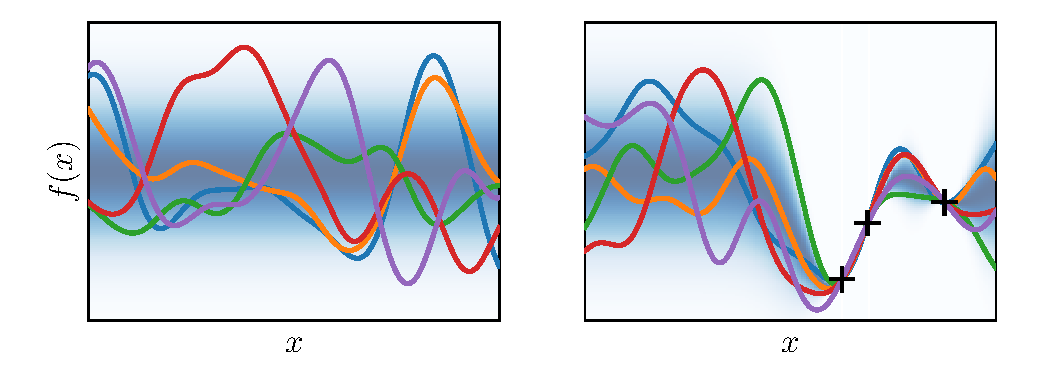
\includegraphics[width=\textwidth]{figures/intro/gp_intro.pdf}
  \caption{Illustration of Gaussian Process Regression in a one-dimensional case.
  The shades of blue represent the distribution of function values at each input point $x$.
  Color lines are random functions sampled from the GP.
  {\em Left}: figure depicts prior distribution over functions with several random
  functions drawn from it.
  {\em Right}: posterior distribution conditioned on several data observations.
  Here the noise in observations is very small, therefore, all posterior samples
  pass through the given points.
  }
  \label{fig:gp_intro}
\end{figure}

The kernel function is central and the most crucial part of GP models.
The type of kernel specifies which class of functions can be approximated by GP
and what peculiarities the model will possess.
By specifying a kernel we can end up with models that are equivalent to other
well known models, like linear regression or splines.
However, in practice usually a squared exponential (it is also often called Radial Basis Function (RBF) kernel) covariance function is used
\begin{equation}
  \label{eq:covariance_function}
  k(\mathbf{x}_p, \mathbf{x}_q) = \sigma_f^2 \exp \left ( -\sum_{i = 1}^d \theta_i^2 (\mathbf{x}_p^{(i)} - \mathbf{x}_q^{(i)})^2 \right ).
\end{equation}
This kernel is infinitely smooth and is shift-invariant,
i.e. $k(\mathbf{x, y}) = k(\mathbf{x - y})$ which has its own advantages and disadvantages.
Nevertheless, this kernel is highly popular and is a universal choice
that works quite well in many applications.


\subsection{Hyperparameters tuning}
One of the appealing property of GP models is that they allow to
carefully tune their hyper-parameters without over-fitting to the observed data.

Let us denote hyper-parameters of the kernel function and noise variance by $\bm{\theta}$.
To choose good $\bm{\theta}$ we consider the log likelihood
\begin{equation}
  \label{eq:loglikelihood}
    \log p(\mathbf{y} \, | \, \mathbf{X}, \boldsymbol{\theta}, \sigma_f, \sigma_{noise}) =
    -\underbrace{\frac12 \mathbf{y}^T \mathbf{K}_y^{-1}\mathbf{y}}_{\text{data fit term}}
    - \underbrace{\frac12 \log |\mathbf{K}_y|}_{\text{complexity term}}
    - \frac{N}{2} \log 2 \pi
\end{equation}
and maximize it over the hyper-parameters \citep{rasmussen2006gaussian}.
The objective is also called {\em marginal log-likelihood} as it implicitly
marginalizes out all function values at other input locations that are not present
in the training set.
There are essentially two terms in the objective function.
One term encourages the data fit and the other one controls the model's complexity.
It allows comparing different models and balance between data interpolation and
the model's capacity.

\section{Features of Gaussian Processes}
GP models have some peculiarities, some of them makes it more attractive, some --- limit their applicability.
\begin{enumerate}
    \item \textbf{Analytical solution}.
      The predictive posterior distribution is given by a simple analytical expression.
      This simplifies analysis of the model and can make it easier to build on top of
      GP model.
      And it is always nice to have a closed-form solution.

    \item \textbf{Marginalization}.
      Marginalization over all function values at locations that are not in the training
      set is actually averaging over a wide range of functions, which
      is actually a strong regularization that makes over-fitting less possible.

    \item \textbf{Flexibility}.
      Different peculiarities of the data set and underlying unknown function
      can be taken into account by considering specific kernel functions.

    \item \textbf{Uncertainty estimation}.
      Predictive distribution allows us to estimate the uncertainty of the prediction.
      It can be required by the application itself as well as used to solve other
      problems, e.g., adaptive Design of Experiments, Bayesian Optimization and others.

    \item \textbf{Well developed theory}.
      GP models have a simple structure and, therefore, have already been
      well studied and many properties have been discovered.
      This makes the models attractive because their behavior can be explained
      theoretically.
      It is also easier to analyze the models that were built on top of GP models.
      Theoretical analysis of the models is essential as it helps to understand
      in what cases the model will or will not work, how to pre-process the data
      or modify the overall approach to make it work and so on.

    \item \textbf{Computational complexity}.
      As it can be seen from \eqref{eq:loglikelihood} we need to calculate the determinant
      and the inverse of the kernel matrix of size $N \times N$.
      Therefore, inference requires $\mathcal{O}(N^3)$ operations, which
      makes it prohibitive to use GP models in case of large data sets.
      Test time evaluation complexity is $\mathcal{O}(N)$ and in some applications it can also
      be too high.
      In Chapter~\ref{chap:gp_on_grids} we show a way to reduce the computational complexity drastically
       for structured data sets,
      and in Chapter~\ref{chap:unstructured_datasets} we consider general unstructured
      data sets and develop an efficient approximation to the kernel function.

    \item \textbf{Kernel choice}. Kernel is the most important part of the GP model.
    It specifies the behavior of the model and a class of functions that can be
    well approximated.
    However, in most cases, we do not know in advance what type of kernel
    best suits the data set at hand and either stick to some universal kernel (like RBF)
    or construct an appropriate kernel manually.
    Nevertheless, there are some works that tries to select the best kernel automatically, for example, \citep{duvenaud2014automatic, abdessalem2017automatic, teng2020scalable}.
    There are works that bypass the kernel design by building Deep Gaussian Processes \citep{damianou2013deep} or
    combine deep networks with Gaussian Processes \citep{wilson2016stochastic}.

    \item \textbf{Gaussian distribution}.
    In GP the distribution of output values (i.e., likelihood) is Gaussian.
    Sometimes the actual likelihood is non-Gaussian, for example, when we deal
    with classification tasks.
    In this case we need to use approximate solutions.
    This direction is well developed and there are several frameworks
    that allows us to work with non-Gaussian likelihoods \citep{de2017gpflow,gardner2018gpytorch} easily.

\end{enumerate}

In the thesis we approach the computational complexity issue.
There is considerable amount of work in this direction
(for example, \citep{quinonero2005unifying,rahimi2008random,titsias2009variational,cutajar2017random}).
Nevertheless, we would like to point that
generally exact Gaussian Process models work better than the existing approximations
\citep{cutajar2016preconditioning,wang2019exact}.
Also, typically large-scale approximate methods have hyper-parameter that controls
the accuracy of the approximation (for example, number of inducing points in \citep{quinonero2005unifying,titsias2009variational}
and number of features in \citep{rahimi2008random,felix2016orthogonal} and their follow-ups).
The analysis of such approaches show that optimal learning rates requires this parameter to be at least $\mathcal{O}(\sqrt{N} \log N)$
\citep{aless2016generalization,rudi2017falkon}.
Therefore, the computational complexity becomes $\mathcal{O}(N\sqrt{N})$ in this case.
In the thesis we prefer to do exact inference when it is possible.
In case of large-scale data sets it can be done if there is a way
to exploit the structure of the problem.
Such approach we develop in Chapter \ref{chap:gp_on_grids} for data sets on multi-dimensional grids
and show that its computational complexity is lower than the complexity of the large-scale approximations.


In case of unstructured data sets the way to build large-scale Gaussian Process model
is to do approximations.
Current state-of-the-art scalable approaches show great effectiveness in real-world
problems.
Better performance is usually achieved by {\em data-dependent} approaches, i.e.
the approaches that rely on the given data set.
On the other hand, in some applications {\em data-independent} techniques are more attractive as
they do not require the data set to construct an approximation.
For example, applications where we data changes frequently, so it is more costly
or less accurate to use data-dependent techniques.
Simultaneous localization and mapping is an example of such problems (we consider it Chapter \ref{chap:applications}).
For this reasons in the thesis we focus on data-independent approach.






\chapter{Gaussian Process Models on Multi-dimensional Grids}
\label{chap:gp_on_grids}


% \todo{Move this part to the intro and background. From here}

% Gaussian Processes (GP) have become a popular tool for regression which has lots of applications
% in engineering problems \citep{rasmussen2006gaussian}.
% They combine flexibility by allowing to approximate a wide range of smooth functions
% with simple structure of Bayesian inference and interpretable hyperparameters.

% GP regression algorithm has $\mathcal{O}(N^3)$ time complexity and $\mathcal{O}(N^2)$
% memory complexity, where $N$ is a size of the training sample.
% For large training sets (ten thousands or more) construction of GP regression becomes intractable
% problem on current hardware.
Let us consider the case when the training set has a special structure
called {\em factorial Design of Experiments} (DoE) \citep{Montgomery2006DAE}.
In this structure all the input variables are grouped into several {\em factors},
and the training set consists of the Cartesian product of the factors.
Such experimental designs arise naturally in many applications, especially in engineering.
Imagine that we want to model some aerodynamic characteristic of an airfoil depending
on the shape of the airfoil and external conditions, like Mach number and angle of attack.
There are two ways to do it.
The first one is to conduction computational fluid dynamic simulation to estimate
the desired characteristics.
Another way is to build an airfoil and conduct wind tunnel experiments.
In the later case it is expensive to build airfoils but easy to change the external
conditions so that we can select the external parameters on a regular grid
for each airfoil.
As a result, we have two sets of parameters.
One set describes the geometry of the airfoil, the other one - external conditions.
And in our measurements those parameters have the Cartesian product structure.
In some cases we can have missing values in such design of experiments.
It can be either to some errors in measurements, computationally unstable procedures,
or just to decrease the data set size.
In this case we have {\em incomplete factorial Design of Experiments}.

The problem with such designs is that the training set size grows exponentially
with the number of factors.
The complexity of standard GP models does not allow to work with such training sets.
There are several methods for large-scale GP modeling, although they are not exact
and approximate either the kernel function or the output of the GP model itself.
These approaches are general and can be applied to any data set.
More details can be found in Chapter~\ref{chap:unstructured_datasets}.

However, in case of full or incomplete factorial DoE the special structure
of the data set can be exploited to derive computationally efficient
and the exact inference procedure.
There are no many regression methods that take into account the design of experiments.
There are several methods based on splines which consider this special structure of the given data \citep{stone97polynomialsplines}.
A disadvantage of these methods is that they work only with one-dimensional factors
and cannot be applied to a more general case when factors are multidimensional.
Another shortcoming is that such approaches do not have approximation accuracy evaluation procedure.
Missing values cannot be handled as well.


There is another problem which we are likely to encounter.
Factor sizes can vary significantly.
Engineers usually use large factors sizes if corresponding input variables have a significant impact on function values
otherwise, the factors sizes are likely to be small,
i.e. the factor sizes are often selected using knowledge from a subject domain \citep{rendall2008aircraftSurface}.
For example, if it is known that dependency on some variable is quadratic,
then the size of this factor will be three as a larger size is redundant.
The difference between factor sizes can lead to the degeneracy of the GP model.
We will refer to this property of data set as {\em anisotropy}.

In this chapter we develop an approach for fast, exact inference of the GP regression
model by taking into account
the factorial nature of the design of experiments in a general case of multidimensional factors.
Both full factorial and incomplete factorial designs are covered.
We also discuss how to choose initial values of parameters for
the GP model and regularization in order to
take into account possible anisotropy of the training data set.

The paper \citep{wilson2014fast} considers the same problem statement.
To efficiently train and evaluate a GP model one needs a fast procedure
to calculate $\mathbf{K}^{-1}\mathbf{y}$,
where $\mathbf{K}$ is a kernel matrix,
and an efficient procedure to evalute the determinant of the kernel matrix.
The authors of \citep{wilson2014fast} exploit the structure in the dataset
to efficiently calculate both components in case of full factorial design of experiments.
In case of incomplete factorial design of experiments
they apply preconditioned conjugate gradient (PCG) method to calculate $\mathbf{K}^{-1}\mathbf{y}$.
It is based on an efficient approach for matrix-vector product $\mathbf{K}\mathbf{y}$
which, however, gives an exact answer only in the limit when the parameter of the method goes to infinity.
Empricially, the PCG in this case requires small number of iterations (much smaller than the dataset size).
In contrast, this chapter of the dissertation shows an approach that calculates
$\mathbf{K}^{-1}\mathbf{y}$ in case of incomplete factorial deign of experiments exactly.
We also derive the exact number of iterations required for conjugate gradients approach to converge.
We show that the method is efficient when the number of missing points is small or very large.
Another difference is that we calculate the determinant of the kernel matrix exactly but in about
$\mathcal{O}(N^2)$ operations, whereas \citep{wilson2014fast} make an approximation to the determinant
but in $\mathcal{O}(N)$ iterations.
We also introduce a special regularization that allows to reduce degeneration effect.



The main contributions of this chapter are as follows
\begin{itemize}
  \item We develop a computationally efficient approach for the case of the multi-dimensional
  data set.
  \item For the case of multi-dimensional grid with missing points we derive a conjugate gradients
  based approach for matrix inversion that provably converges in $\mathcal{O}(\min (R, N))$
  iterations, where $R$ is the number of missing points.
  \item We propose a special regularization for the data sets on multi-dimensional grids
  that makes the GP model less prone to degeneration.
\end{itemize}

% In this chapter we consider the data sets with special structure.
% We suppose that input variables are grouped into several sets and
% input points form the Cartesian product of the sets.
% Such designs of the experiment are called {\em factorial design of experiments} (DoE) and
% common in many engineering problems \citep{Montgomery2006DAE}.
% The sets of groups of variables are called {\em factors}.
% Number of different values in a factor is called {\em factor size}.

% When the factorial DoE is used the size of the data set can be very large
% as it grows exponentially with dimension of input variables.
% We also consider problems where some points are missing from the
% Cartesian product.
% However, in both cases an efficient algorithm can be constructed
% by taking into account the structure of the dataset.


\section{Factorial design of experiments}
Let us refer to sets of points
${\omega_k = \{ x_{i_k}^k \in {\rm X}_k \}_{i_k = 1}^{n_k}}$,
${\rm X}_k \subset \mathbb{R}^{d_k}, \, k = \overline{1, K}$ as {\em factors}.
A set of points $\Omega$ is referred to as a factorial design of experiments
if it is a Cartesian product of factors
\begin{equation}
  \label{eq:factorial_design}
    \Omega = \omega_1 \times \omega_2 \times \cdots \times \omega_k =
    \{ [x_{i_1}^1, \ldots, x_{i_K}^K], \{ i_k = 1, \ldots, n_k\}_{k = 1}^K \}.
\end{equation}
The elements of $\Omega$ are vectors of a dimension $d = \sum_{i = 1}^K d_i$ and
the sample size is a product of sizes of all factors $N = \prod_{i = 1}^K n_i$.
If all the factors are one-dimensional $\Omega$ is a full factorial design.
But in a more general case factors are multidimensional (see example in Figure \ref{fig:multidim_factor}).

\begin{figure}
  \centering
  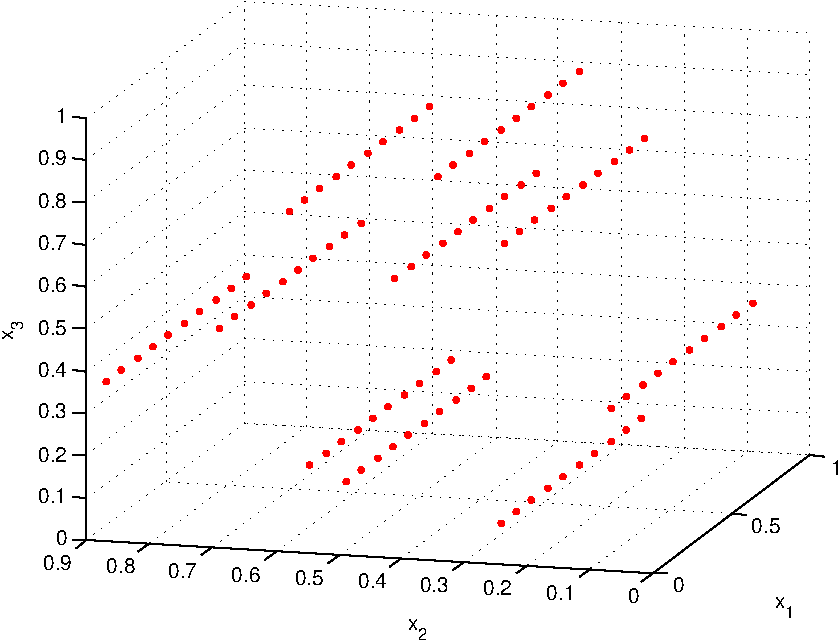
\includegraphics[width=0.5\textwidth]{figures/gp_on_grid/multidim_factor.pdf}
  \caption{Example of a multidimensional factor. In the figure $x_1$ is a usual one-dimensional factor
  and $(x_2, x_3)$ is a 2-dimensional factor.}
  \label{fig:multidim_factor}
\end{figure}


\section{Tensor and related operations}
Let us introduce tensor notation and some related operations that will be used
later.

A {\em tensor} $\mathcal{Y}$ is a $K$-dimensional matrix of size $n_1 \times n_2 \times \cdots \times n_K$
\citep{kolda09tensordecompositions}:
\begin{equation}
  \label{eq:tensor}
  \mathcal{Y} = \{ y_{i_1, i_2, \ldots, i_K}, \{i_k = 1, \ldots, n_k \}_{k = 1}^K \}.
\end{equation}

By $\mathcal{Y}^{(j)}$ we will denote a matrix consisting of elements of the tensor $\mathcal{Y}$
whose rows are $1 \times n_j$ slices of $\mathcal{Y}$ with fixed indices
$i_{j + 1}, \ldots, i_K, i_1, \ldots, i_{j - 1}$ and altering index $i_j = 1, \ldots, n_j$.
In case of $2$-dimensional tensor it holds that
${\mathcal{Y}^{(1)} = \mathcal{Y}^T}$ and $\mathcal{Y}^{(2)} = \mathcal{Y}$.

Now let us introduce multiplication of a tensor by a matrix along the direction $i$.
Let $B$ be some matrix of size $n_i \times n_i'$.
Then the product of the tensor $\mathcal{Y}$ and the matrix $B$ along the direction $i$
is a tensor $\mathcal{Z}$ of size $n_1 \times \cdots \times n_{i - 1} \times n_i' \times n_{i + 1} \times \cdots \times n_K$
such that $\mathcal{Z}^{(i)} = \mathcal{Y}^{(i)}B$.
We will denote this operation by $\mathcal{Z} = \mathcal{Y} \otimes_i B$.
For a $2$-dimensional tensor $\mathcal{Y}$ multiplication along the first direction is a left multiplication
by matrix $\mathcal{Y} \otimes_1 B = B^T \mathcal{Y}$,
and along the second direction --- is a right multiplication $\mathcal{Y} \otimes_2 B = \mathcal{Y} B$.

Multiplication of a tensor by a matrix along some direction is closely related to the Kronecker product.
Let's consider an operation {\em vec} which for every multidimensional matrix $\mathcal{Y}$
returns a vector containing all elements of $\mathcal{Y}$.
An inner product of tensors $\mathcal{Y}$ and $\mathcal{Z}$ is the inner product of vectors
${\rm vec}(\mathcal{Y})$ and ${\rm vec}(\mathcal{Z})$
\[
\left < \mathcal{Y}, \mathcal{Z}\right > = \left < {\rm vec}(\mathcal{Y}), {\rm vec}(\mathcal{Z}) \right >.
\]

For every multidimensional matrix $\mathcal{Y}$ of size $n_1 \times n_2 \times \cdots \times n_K$
and $n_i \times p_i$ size matrices $B_i$, $i = 1, \ldots, K$ the following identity holds \citep{loan2000kronecker}
\begin{equation}
  \label{eq:kronecker_product}
    (B_1 \otimes B_2 \cdots \otimes B_K) {\rm vec}(\mathcal{Y}) =
    {\rm vec} (\mathcal{Y} \otimes_1 B_1^T \cdots \otimes_K B_K^T),
\end{equation}
where symbol $\otimes$ denotes the Kronecker product.

Let's compare a complexity of the right and the left hand sides of (\ref{eq:kronecker_product}).
For simplicity we assume that all the matrices $B_i$ are quadratic of size $n_i \times n_i$ and
$N = \prod n_i$.
Then computation of the left-hand side of (\ref{eq:kronecker_product}) requires
$N^2$ operations (of additions and multiplications) not taking into account the complexity of the Kronecker product
while the right hand side requires $N \sum_i n_i$ operations.


\subsection{Efficient log-likelihood calculation}
\label{sec:calc_loglikelihood}
Now, let us see how the introduced operations can be used for efficient
computation of the predictive distribution and the marginal log-likelihood.

Covariance function (\ref{eq:covariance_function}) can be represented as
a product of covariance functions each depending only on variables from one factor
\begin{equation}
  \label{eq:covariance_function_general}
  k(\mathbf{x}_p, \mathbf{x}_q) = \prod_{i = 1}^K k_i(x_p^i, x_q^i),
\end{equation}
where $x_p^i, x_q^i \in \mathbb{R}^{d_i}$ belong to the same factor $\omega_i$.
For the squared exponential function we have $k_i(x_p^i, x_q^i) = \omega_{f, i}^2\exp \left ( -\sum_j^{d_i} \left (\theta_i^{(j)} \right )^2
  \big (x_p^{(j), i} - x_q^{(j), i} \big )^2 \right )$,
where $x_p^{(j), i}$ is a $j$-th component of $x_p^i$.
Note that in general case covariance functions $k_i$ are not necessarily squared exponential, they can be of different types for different factors.
It allows to take into account special features of factors (knowledge from a subject domain) if they are known.
In such case the function defined by (\ref{eq:covariance_function_general}) is still a valid
covariance function being the product of separate covariance functions.
From now on we will denote by $\theta_i = (\theta_i^{(1)}, \ldots, \theta_i^{(d_i)})$ the set of hyperparameters for covariance
function of the $i$-th factor and let $\boldsymbol{\theta} = (\theta_1, \ldots, \theta_K)$.

Such form of the covariance function and the factorial DoE
allows us to represent the covariance matrix as the Kronecker product
\begin{equation}
  \label{eq:covariance_kronecker}
  \mathbf{K}_f = \bigotimes_{i = 1}^K\mathbf{K}_i,
\end{equation}
where $\mathbf{K}_i$ is a covariance matrix defined by the $k_i$ covariance function
computed at points from the $i$-th factor $\omega_i$.

The Kronecker product of matrices can be efficiently inverted due to the following
property
\[
(A \otimes B)^{-1} = A^{-1} \otimes B^{-1}
\]
if $A$ and $B$ are invertible matrices.
If $A$ has size $n_a \times n_a$ and $B$ has size $n_b \times n_b$ then
the left side of the above equation requires $\mathcal{O}(n_a^3n_b^3)$ operations
while the right hand side requires only $\mathcal{O}(n_a^3 + n_b^3)$ operations
and this is much less.
However, we have to invert the matrix $\mathbf{K}_y = \mathbf{K}_f + \sigma_{noise}^2 \mathbf{I}$.
For this we will use the Singular Value Decomposition (SVD)
\[
\mathbf{K}_i = \mathbf{U}_i \mathbf{D}_i \mathbf{U}_i^T,
\]
where $\mathbf{U}_i$ is an orthogonal matrix of eigenvectors of matrix $\mathbf{K}_i$
and $\mathbf{D}_i$ is a diagonal matrix of eigenvalues.
Using the properties of the Kronecker product and representing an identity matrix as
$\mathbf{I}_{d_i} = \mathbf{U}_i \mathbf{U}_i^T$ we obtain
\begin{equation}
  \label{eq:inverse_covariance}
  \mathbf{K}_y^{-1} = \left (\bigotimes_{i = 1}^K \mathbf{U}_i \right ) \left (
    \left [\bigotimes_{i = 1}^K \mathbf{D}_i \right ] + \sigma_{noise}^2 \mathbf{I} \right )^{-1}
  \left ( \bigotimes_{i = 1}^K \mathbf{U}_i^T \right ).
\end{equation}

Computing SVD for all $\mathbf{K}_i$ requires $\mathcal{O}(\sum_k n_k^3)$ operations.
Calculation of the Kronecker product in (\ref{eq:inverse_covariance}) has complexity $\mathcal{O}(N^2)$.
So, this gives us overall complexity $\mathcal{O}(N^2)$ for calculation of expressions for the log-likelihood,
the predictive mean and the covariance.
It is faster than the straightforward calculations, however, it can be improved.

Equations~\eqref{eq:gp_posterior} and \eqref{eq:loglikelihood}
for GP regression do not require explicit inversion of $\mathbf{K}_y$.
In each equation it is multiplied by vector $\mathbf{y}$ (or $\mathbf{k}_*$).
So, we will compute $\mathbf{K}_y^{-1} \mathbf{y}$ instead of explicitly inverting
$\mathbf{K}_y$ and then multiplying it by the vector $\mathbf{y}$.

Let $\mathcal{Y}$ be a tensor containing values of the vector $\mathbf{y}$ such that
${\rm vec}(\mathcal{Y}) = \mathbf{y}$.
Now using identities (\ref{eq:kronecker_product}) and (\ref{eq:inverse_covariance})
we can write $\mathbf{K}_y^{-1}\mathbf{y}$ as
\begin{align}
  \label{eq:fast_inverse_covariance}
    \mathbf{K}_y^{-1}\mathbf{y} &= \left ( \bigotimes_{i = 1}^K \mathbf{U}_i \right )
    \left ( \left [\bigotimes_{i = 1}^K \mathbf{D}_i \right ] + \sigma_{noise}^2 \mathbf{I} \right )^{-1} \times
    {\rm vec}(\mathcal{Y} \otimes_1 \mathbf{U}_1 \cdots \otimes_K \mathbf{U}_K) = \nonumber \\
    &= {\rm vec}\left [ \left ((\mathcal{Y} \otimes_1 \mathbf{U}_1 \cdots \otimes_K \mathbf{U}_K) * \mathcal{D}^{-1} \right ) \otimes_1
    \mathbf{U}_1^T \cdots \otimes_K \mathbf{U}_K^T \right ],
\end{align}
where $\mathcal{D}$ is a tensor constructed by transforming the diagonal of matrix
$\big [\bigotimes_k \mathbf{D}_k \big ] + \sigma_{noise}^2 \mathbf{I}$ into a tensor.

The elements of the tensor $\mathcal{D}$ are eigenvalues of the matrix $\mathbf{K}_y$,
therefore its determinant can be calculated as
\begin{equation}
  \label{eq:fast_determinant}
  |\mathbf{K}_y| = \prod_{i_1, \ldots, i_K} \mathcal{D}_{i_1, \ldots, i_K}.
\end{equation}

\begin{proposition}
  The computational complexity of the log likelihood (\ref{eq:loglikelihood}), where $\mathbf{K}_y^{-1}y$ and
  $|\mathbf{K}_y|$ are calculated using (\ref{eq:fast_inverse_covariance}) and (\ref{eq:fast_determinant}), is
  \begin{equation}
    \mathcal{O} \left (\sum_{i = 1}^K n_i^3 + N\sum_{i = 1}^K n_i \right ).
  \end{equation}
\end{proposition}
\begin{proof}
  Let's calculate the complexity of computing $\mathbf{K}_y^{-1} \mathbf{y}$ using (\ref{eq:fast_inverse_covariance}).
  Computation of the matrices $\mathbf{U}_i$ and $\mathbf{D}_i$ requires $\mathcal{O}(\sum_i n_i^3)$ operations.
  Multiplication of the tensor $\mathcal{Y}$ by the matrices $\mathbf{U}_i$ requires $\mathcal{O}(N\sum_i n_i)$ operations.
  Further, a component-wise product of the obtained tensor and the tensor $\mathcal{D}^{-1}$ requires $\mathcal{O}(N)$
  operations.
  And the complexity of multiplication of the result by the matrices $\mathbf{U}_i$ is again $\mathcal{O}(N\sum_i n_i)$.
  The determinant, calculated by equation (\ref{eq:fast_determinant}), requires $\mathcal{O}(N)$ operations.
  Thus, the overall complexity of computing (\ref{eq:fast_inverse_covariance}) is
  ${\mathcal{O}(\sum_{i = 1}^K n_i^3 + N\sum_{i = 1}^K n_i)}$.
\end{proof}

For more illustrative estimate of the computational complexity
suppose that $n_i \ll N$ (number of factors is large and their sizes are close).
In this case it holds that
$\mathcal{O}(N\sum_i n_i) = \mathcal{O}(N^{1 + \frac{1}{K}})$ and this is
much less than $\mathcal{O}(N^3)$.

To optimize the log-likelihood over the hyperparameters, we use a gradient-based method.
The derivatives of the log likelihood with respect to the hyperparameters take the form
\begin{equation}
\label{eq:loglikelihood_derivative}
    \frac{\partial}{\partial \theta} \left (\log \vphantom{p(\mathbf{y} | \mathbf{X}, \sigma_f, \sigma_{noise})}
    p(\mathbf{y} | \mathbf{X}, \sigma_f, \sigma_{noise}) \right ) =
    -\frac12 {\rm Tr}(\mathbf{K}_y^{-1} \mathbf{K}') + \frac12\mathbf{y}^T \mathbf{K}_y^{-1} \mathbf{K}' \mathbf{K}_y^{-1} \mathbf{y},
\end{equation}
where $\theta$ is one of the hyperparameters $\theta_i$, $\sigma_{noise}$ or $\omega_{f, i}, i = 1, \ldots, d$ and
$\mathbf{K}' = \dfrac{\partial \mathbf{K}}{\partial \theta}$.
$\mathbf{K}'$ is also the Kronecker product
\[
\mathbf{K}' = \mathbf{K}_1 \otimes \cdots \otimes \mathbf{K}_{i - 1} \otimes \frac{\partial \mathbf{K}_i}{\partial \theta}
\otimes \mathbf{K}_{i + 1} \otimes \cdots \otimes \mathbf{K}_K,
\]
where $\theta$ is a parameter of the $i$-th covariance function.
Denoting by $\mathcal{A}$ a tensor such that ${\rm vec}(\mathcal{A}) = \mathbf{K}_y^{-1}\mathbf{y}$
the second term in equation (\ref{eq:loglikelihood_derivative}) can be efficiently computed
using the same technique as in (\ref{eq:fast_inverse_covariance}):
\begin{align}
  \label{eq:fast_derivative_second_term}
    \frac12\mathbf{y}^T \mathbf{K}_y^{-1} \mathbf{K}'\mathbf{K}_y^{-1} \mathbf{y} =
    \left < \mathcal{A}, \mathcal{A}
    \vphantom{\frac{\partial \mathbf{K}_i^T}{\partial \theta}}
    \right .
    & \otimes_1 \mathbf{K}_1^T \otimes_2 \cdots \otimes_{i - 1}
    \mathbf{K}_{i - 1}^T \otimes_i
    \frac{\partial \mathbf{K}_i^T}{\partial \theta} \otimes_{i + 1} \nonumber \\
    &\left .
    \vphantom{\frac{\partial \mathbf{K}_i^T}{\partial \theta}}
    \otimes_{i + 1} \mathbf{K}_{i + 1}^T \otimes_{i + 2} \cdots \otimes_K \mathbf{K}_K^T \right >.
\end{align}
The complexity of calculating this term of derivative is the same as the complexity of
equation (\ref{eq:fast_inverse_covariance}).

Now let's compute the first term
\begin{equation}
  \begin{split}
    {\rm Tr}(\mathbf{K}_y^{-1} \mathbf{K}') = &\; {\rm Tr} \left (
      \left (\bigotimes_{i = 1}^K \mathbf{U}_i \right ) \mathbf{D}^{-1} \left (\bigotimes_{i = 1}^K \mathbf{U}_i^T \right ) \mathbf{K}'
    \right)= \\
    = &\; {\rm Tr} \left (\mathbf{D}^{-1} \left (\bigotimes_{i = 1}^K \mathbf{U}_i^T \mathbf{K}_i' \mathbf{U}_i \right ) \right ) = \\
    = &\; \left < {\rm diag} \left (\mathbf{D}^{-1} \right ), {\rm diag} \left (\bigotimes_{i = 1}^K \mathbf{U}_i \mathbf{K}_i' \mathbf{U}_i \right ) \right > = \\
    = &\; \left < {\rm diag} \left (\mathbf{D}^{-1} \right ),  \bigotimes_{i = 1}^K {\rm diag} \left ( \mathbf{U}_i \mathbf{K}_i' \mathbf{U}_i \right ) \right >,
  \end{split}
\end{equation}
where ${\rm diag}\big(A \big)$ is a vector of diagonal elements of a matrix $A$,
$\; \mathbf{D} = \bigotimes_i \mathbf{D}_i + \sigma_{noise}^2 \mathbf{I}$.


The computational complexity of this derivative term is the same as the computational
complexity of equation (\ref{eq:fast_derivative_second_term}).

Thus, we obtain
\begin{proposition}
  The computational complexity of calculating derivatives of the log likelihood is
  ${\mathcal{O}\left (\sum\limits_{i = 1}^K n_i^3 + N \sum\limits_{i = 1}^K n_i \right )}$.
\end{proposition}

\begin{table}[t]
  \caption{Runtime (in seconds) of tensored GP and original GP algorithms.}
  \label{tb:runtime}
  \vskip 0.15in
  \begin{center}
    \begin{small}
      \begin{sc}
        \begin{tabular}{rrr}
          \hline
          %\abovespace\belowspace
          & original GP   & tensored GP \\
          64     & 0.8    & 0.16 \\
          160    & 2.69   & 0.16 \\
          432    & 14.31  & 0.74 \\
          1000   & 120.38 & 1.02 \\
          2000   & 970.21 & 1.11 \\
          10240  & ---    & 33.18 \\
          64000  & ---    & 74.9 \\
          160000 & ---    & 175.15 \\
          400000 & ---    & 480.14\\
          \hline
          %\abovespace\belowspace
        \end{tabular}
      \end{sc}
    \end{small}
  \end{center}
  \vskip -0.1in
\end{table}

Table \ref{tb:runtime} contains training times for
original GP and proposed GP regression for different sample sizes.
The experiments were conducted on a PC with Intel i7 2.8 GHz processor and
4 GB RAM.
For original GP we used GPML Matlab code \citep{gpmltoolbox}.
We also adopted the GPML code to use tensor operations.
The results illustrate that the proposed approach is much faster than the original GP
and allows making approximations using extremely large data sets.

\subsection{Anisotropy}
In this section, we will consider an anisotropy problem.
As it was mentioned in an engineering practice factorial designs are
often anisotropic, i.e., sizes of factors differ significantly.
It is a common case for the GP regression to become degenerate in such a situation.
Suppose that the given DoE consists of two one-dimensional factors
with sizes $n_1$ and $n_2$.
Assume that $n_1 \ll n_2$.
Then one could expect the length-scale for the first factor to be much greater than
the length-scale for the second factor (or $\theta_1 \ll \theta_2$).
However, in practice we often observe the opposite $\theta_1 \gg \theta_2$.
This happens because the optimization algorithm stacks in a local maximum during maximization over
the hyperparameters as the objective function (the log-likelihood) is non-convex with lots of local maxima.
We get an undesired effect of degeneracy:
in the region without training points the approximation is constant, and it has sharp peaks at training points.
This situation is illustrated in Figure \ref{fig:anisotropy_degeneracy}
(compare with the true function in Figure \ref{fig:anisotropy_degeneracy_true}).

Let us denote length-scales as $l_k^{(i)} = \big [\theta_k^{(i)} \big ]^{-1}$.
To incorporate our prior knowledge about factor sizes into regression model
we introduce prior distribution on the hyperparameters~$\boldsymbol{\theta}$:
\begin{equation}
  \label{eq:prior}
  \frac{\theta_k^{(i)} - a_k^{(i)}}{b_k^{(i)} - a_k^{(i)}} \sim \mathcal{B}e(\alpha, \beta), \, \{ i = 1, \ldots, d_k\}_{k = 1}^K,
\end{equation}
i.e. prior on hyperparameter $\theta_k^{(i)}$ is a beta distribution with parameters $\alpha$
and $\beta$ scaled to some interval $\left [a_k^{(i)}, b_k^{(i)} \right ]$.

The log likelihood then has the form
\begin{equation}
  \label{eq:loglikelihood_prior}
  \begin{split}
    \log p(\mathbf{y} \, | \, \mathbf{X}, \boldsymbol{\theta}, \sigma_f, \sigma_{noise}) = -& \frac12 \mathbf{y}^T \mathbf{K}_y^{-1}\mathbf{y} - \frac12 \log |\mathbf{K}_y| - \\
    - \frac{N}{2} \log 2 \pi + & \sum_{k, i} \left ( (\alpha - 1) \log(\theta_k^{(i)}) + \right . \\
    + (\beta - 1) \log (1 - &  \left . \theta_k^{(i)})  \right ) - d \log({\rm B}(\alpha, \beta)),
  \end{split}
\end{equation}
where ${\rm B}(\alpha, \beta)$ is a beta function.

By introducing such prior we restrict parameters $\theta_k^{(i)}$ to belong
to some interval $\left [a_k^{(i)}, b_k^{(i)} \right ]$ (or length-scales $l_k^{(i)}$ to belong to the interval
$\left [\big (b_k^{(i)} \big)^{-1}, \big (a_k^{(i)} \big )^{-1} \right ]$).
It seems reasonable that for an approximation to fit the training points
the length-scale is not needed to be much less than the distance between points.
That's why we choose the lower bound for the length-scale $l_k^{(i)}$ to be $c_k * \min\limits_{x, y \in \omega_k, x^{(i)} \ne y^{(i)}} ||x^{(i)} - y^{(i)}||$
and the upper bound for the length-scale to be ${C_k * \max\limits_{x, y \in \omega_k} ||x^{(i)} - y^{(i)}||}$.
The value $c_k$ should be close to 1.
If it is chosen too small, we are taking risks to overfit the data by allowing small length-scales.
If $c_k$ is too large, we will underfit the data by allowing only large length-scales and forbidding small ones.
Constants $C_k$ must be much greater than $c_k$ to permit large length-scales and preserve flexibility.
In this work we used $c_k = 0.5$ and $C_k = 100$.
Such values of $c_k$ and $C_k$ worked rather well in our test cases.

Parameters of beta distribution was set to $\alpha = \beta = 2$ to get
symmetrical probability distribution function (see Figure \ref{fig:beta}) because
we do not know a priori large or small should be the values of GP parameters.
Chosen prior distribution penalizes too large and too small values of parameters $\theta_k$
as they are undesirable.

Figure \ref{fig:nondegenerate_tensorGP} illustrates approximation
of the GP regression with introduced prior distribution (and initialization described in Section \ref{sec:tensor_gp_init}).
The hyperparameters were chosen such that the approximation
is nondegenerate.

\begin{figure}
  \centering
  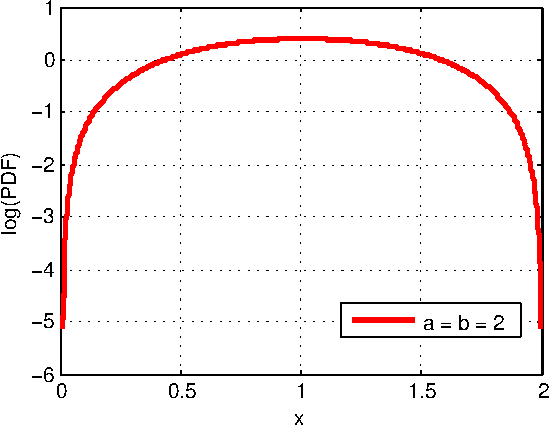
\includegraphics[width=0.3\textwidth]{figures/gp_on_grid/beta.pdf}
  \caption{Logarithm of Beta distribution probability density function, rescaled to $[0.01, 2]$ interval,
    with parameters $\alpha = \beta = 2$.}
  \label{fig:beta}
\end{figure}


\subsection{Initialization}
\label{sec:tensor_gp_init}
It is also important to choose reasonable initial values of hyperparameters
in order to converge to a good solution during parameter optimization.
The kernel-widths for different factors should have different scales because
corresponding factor sizes have a different number of levels.
So it seems reasonable to use average distance between points in a factor as an initial value
\begin{equation}
  \label{eq:initialization}
  \theta_k^{(i)} = \left [ \frac{1}{n_k} \left ( \max\limits_{x \in \omega_k}(x^{(i)}) - \min\limits_{x \in \omega_k}(x^{(i)}) \right ) \right ]^{-1}.
\end{equation}
% i.e. the initial length-scale is an average distance between neighboring points in factor.

\begin{figure}
  \centering
  \begin{subfigure}[b]{0.45\textwidth}
      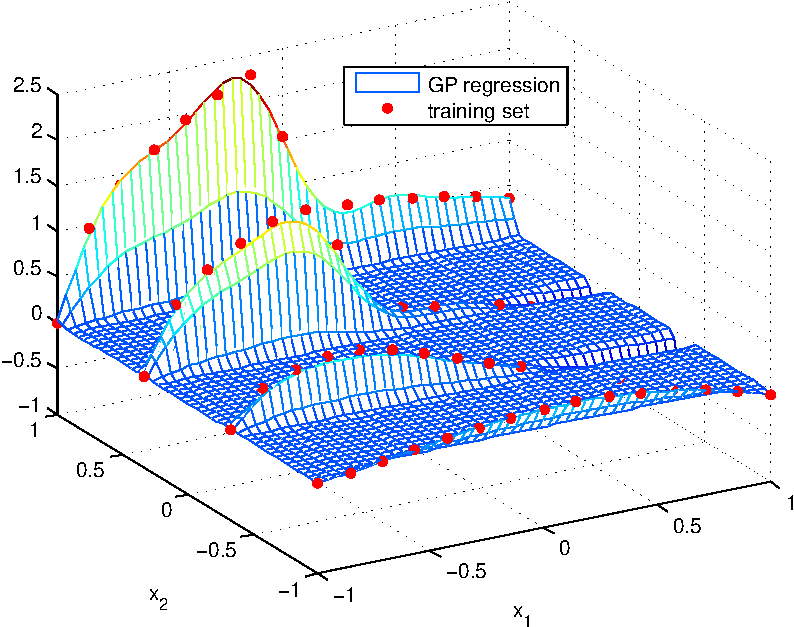
\includegraphics[width=\textwidth]{figures/gp_on_grid/degeneration.pdf}
      \caption{Degeneracy of the GP model in case of anisotropic data set.
        The length-scales for this model are $l_1 = 0.286, l_2 = 0.033$
        whereas factor sizes are $n_1 = 15, n_2 = 4$.}
      \label{fig:anisotropy_degeneracy}
  \end{subfigure}
  \begin{subfigure}[b]{0.45\textwidth}
      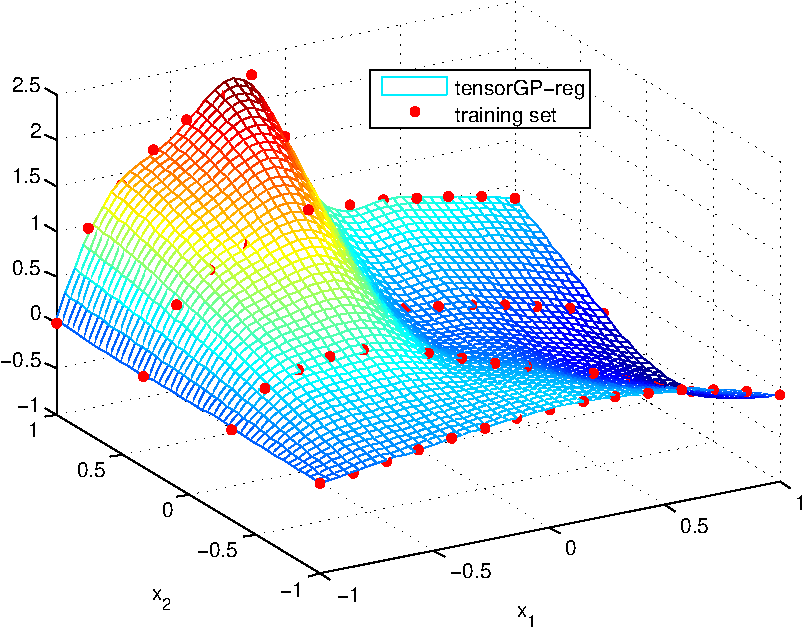
\includegraphics[width=\textwidth]{figures/gp_on_grid/nondegenerate_tensorGP.pdf}
      \caption{The GP regression with proposed prior distribution and initialization.}
      \label{fig:nondegenerate_tensorGP}
  \end{subfigure}
  \begin{subfigure}[b]{0.45\textwidth}
      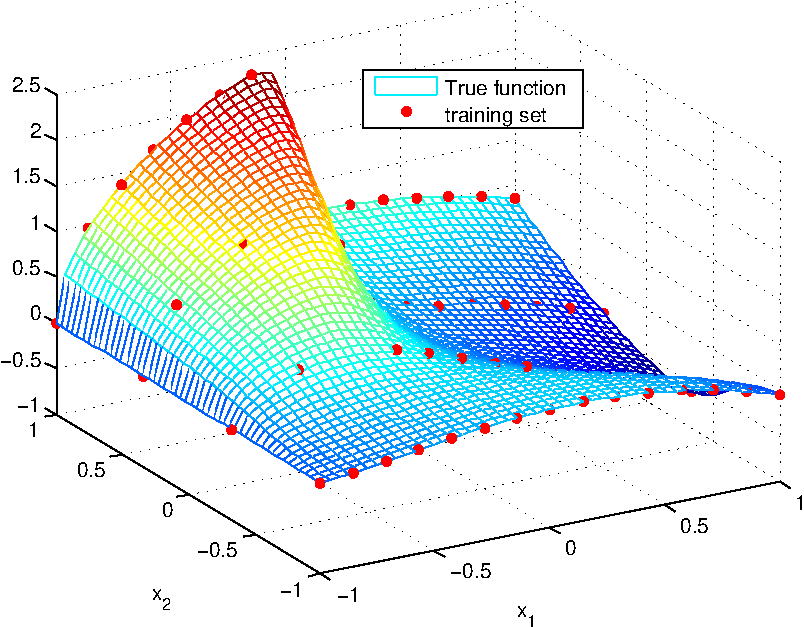
\includegraphics[width=\textwidth]{figures/gp_on_grid/degeneration_true.pdf}
      \caption{True function.}
      \label{fig:anisotropy_degeneracy_true}
  \end{subfigure}
\end{figure}


\section{Experiments}
The proposed algorithm was tested on a set of test functions \citep{lappeenranta, ETH}.
The functions have different input dimensions from 2 to 6 and the sample sizes $N$
varied from $100$ to about $200000$.
For each function several factorial anisotropic training sets were generated.
We will test the following algorithms: GP with tensor computations (tensorGP),
GP with tensor computations and prior distribution (tensorGP-reg),
the sparse pseudo-point input GP (FITC) \citep{snelson06sparsegaussian}.
For FITC method we used GPML Matlab code \citep{gpmltoolbox}.
The number of inducing points of FITC algorithm varied from $M = 500$ for small samples (up to $5000$ points)
to $M = 70$ for large samples (about $10^5$ points) in order to obtain approximation in reasonable time
(complexity of FITC algorithm is $\mathcal{O}(M^2N)$).
For tensorGP and tensorGP-reg we adopted GPML code to use tensor operations, proposed prior distribution
and initialization.

To assess quality of approximation a mean squared error was used
\begin{equation}
  \label{eq:mse}
  {\rm MSE} = \frac{1}{N_{test}} \sum_{i = 1}^{N_{test}} (\hat{f}(\mathbf{x}_i) - f(\mathbf{x}_i))^2.
\end{equation}

To compare different algorithms Dolan-Mor\'{e} curves are used \citep{dolanMore}.
The idea of Dolan-Mor\'{e} curves is as follows.
Let $t_{p, a}$ be an error of an $a$-th algorithm on a $p$-th problem and $r_{p, a}$
be a performance ratio
\[
r_{p, a} = \frac{t_{p, a}} {\min\limits_s(t_{p, s})}.
\]
Then Dolan-Mor\'{e} curve is a graph of $\rho_a(\tau)$ function where
\[
\rho_a(\tau) = \frac{1}{n_p}{\rm size} \{p: r_{p, a} \le \tau \},
\]
which can be thought of as a probability for the  $a$-th algorithm to have performance
ratio within factor $\tau \in \mathbb{R}_+$.
The higher the curve $\rho_a(\tau)$ is located, the better works the corresponding algorithm.
$\rho_a(1)$ is a number of problems on which the $a$-th algorithm showed the best performance.

As expected, tensorGP performs better than FITC as it uses all the information
containing in the training sample.
The introduced prior distribution is more suited for anisotropic data that is why
GP with such prior (tensorGP-reg) performs even better (see Figure \ref{fig:dolan_more}).

To compare run-time performances of the algorithms we plotted Dolan-Mor{'e} curves
where instead of approximation error the training time was used (see Figure \ref{fig:dolan_more_time}).
Here we see that tensorGP and tensorGP-reg outperform FITC algorithm.

\begin{figure}
  \centering
  \begin{subfigure}[b]{0.45\textwidth}
      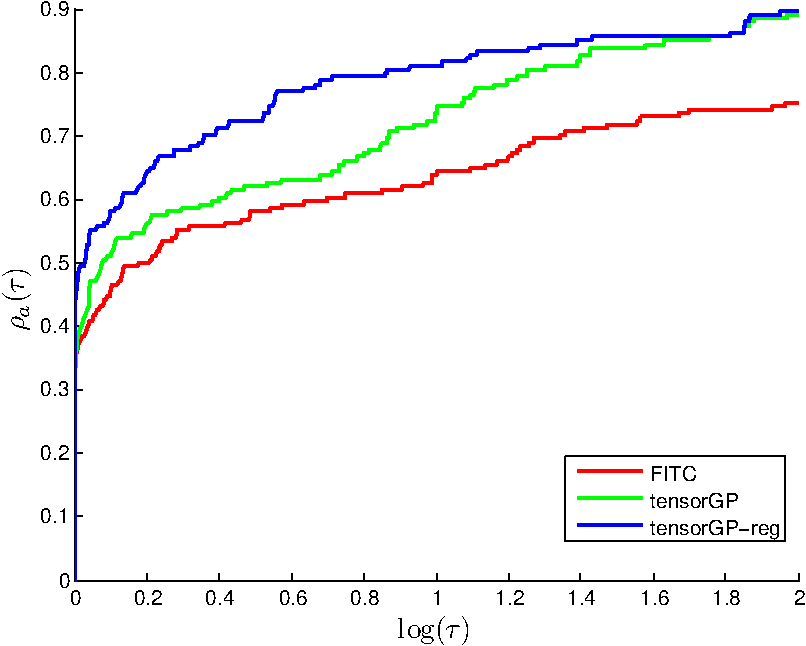
\includegraphics[width=\textwidth]{figures/gp_on_grid/dolan_more.pdf}
      \caption{Approximations accuracy.}
      \label{fig:dolan_more}
  \end{subfigure}
  \begin{subfigure}[b]{0.45\textwidth}
      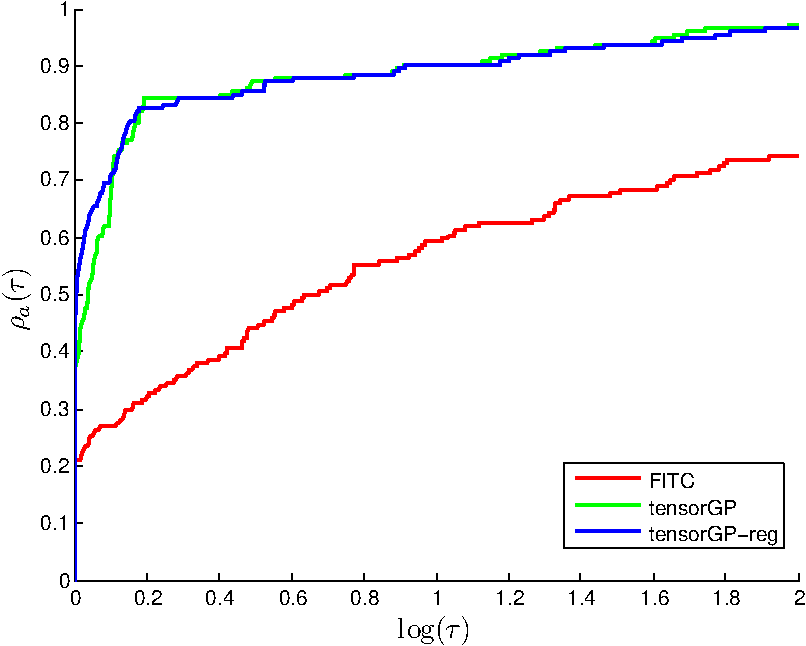
\includegraphics[width=\textwidth]{figures/gp_on_grid/dolan_more_time.pdf}
      \caption{Run-times.}
      \label{fig:dolan_more_time}
  \end{subfigure}
  \caption{Dolan-Mor\'e curves for tensorGP, tensorGP-reg and FITC algorithms
        in logarithmic scale.
        The higher lies the curve, the better performs the corresponding algorithm.}
\end{figure}

\subsection{Rotating disc problem}

In this section we will consider a real-world problem of rotating disc shape design.
Such kind of problems often arises during aircraft engine design and in turbomachinery \citep{armand1995structural}.

In this problem a disc of an impeller is considered.
It is rotated around the shaft.
The geometrical shape of the disc considered here is parameterized by 6 variables
$\mathbf{x} = (h_1, h_2, h_3, h_4, r_2, r_3)$ ($r_1$ and $r_4$ are fixed), see Figures \ref{fig:rotating_disc_parametrization} and \ref{fig:rotating_disc_objectives}.
The task of an engineer is to find such geometrical shape of the disc that minimizes disc's weight and contact pressure $p_1$ between
the disc and the shaft while constraining the maximum radial stress $Sr_{max}$ to be less than some threshold.
The physical model of a rotating disc is described in \citep{armand1995structural} and it was adopted to the disc shape
presented in Figures \ref{fig:rotating_disc_parametrization}, \ref{fig:rotating_disc_objectives} in order to calculate the contact pressure $p_1$
and the maximum radial stress $Sr_{max}$.

\begin{figure}
  \centering
  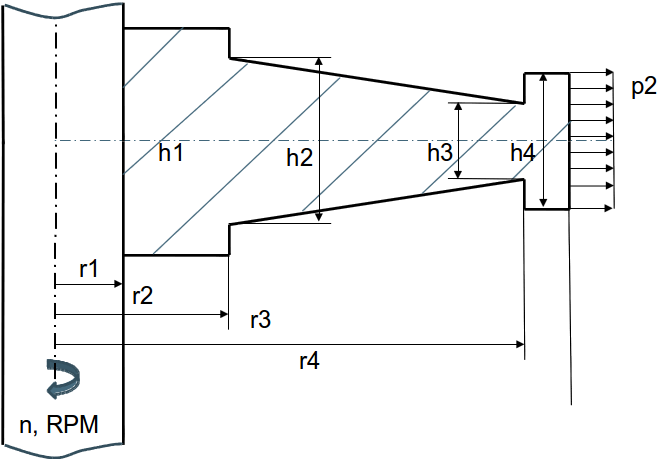
\includegraphics[width=0.4\textwidth]{figures/gp_on_grid/rotating_disk_parametrization.png}
  \caption{Rotating disc parametrization.}
  \label{fig:rotating_disc_parametrization}
\end{figure}

\begin{figure}
  \centering
  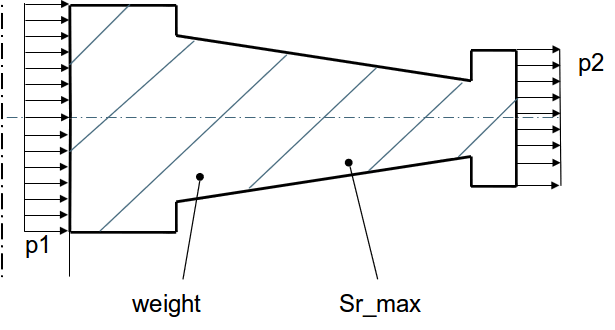
\includegraphics[width=0.4\textwidth]{figures/gp_on_grid/rotating_disk_objectives.png}
  \caption{Rotating disc objectives.}
  \label{fig:rotating_disc_objectives}
\end{figure}

It is a common practice to build approximations of objective functions in order to analyze them
and perform optimization \citep{forrester2008surrogateModelling}.
So, we applied the developed in this work tensorGP-reg algorithm and FITC to this problem.
The DoE was full factorial, the number of points in each dimension was $[1, 8, 8, 3, 15, 5]$, i.e.
$x_1$ was fixed.
The number of points in factors differs significantly and the generated data set is anisotropic.
The overall number of points in the training sample was 14 400.

Figures \ref{fig:rotating_disc_originalGP} and \ref{fig:rotating_disc_tensorGP} depict 2D slices of contact pressure
approximations along $x_5, x_6$ variables.
As you can see FITC model degenerates while tensorGP-reg provides a smooth and accurate approximation.

\begin{figure}
  \centering
  \begin{subfigure}[b]{0.45\textwidth}
      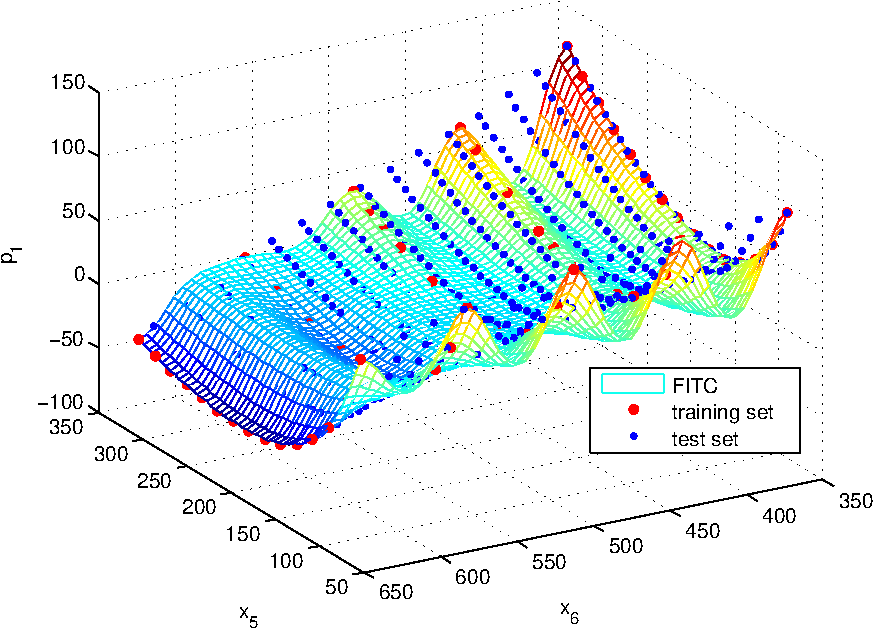
\includegraphics[width=\textwidth]{figures/gp_on_grid/rotating_disk_fitc.pdf}
      \caption{FITC.}
      \label{fig:rotating_disc_originalGP}
  \end{subfigure}
  \begin{subfigure}[b]{0.45\textwidth}
      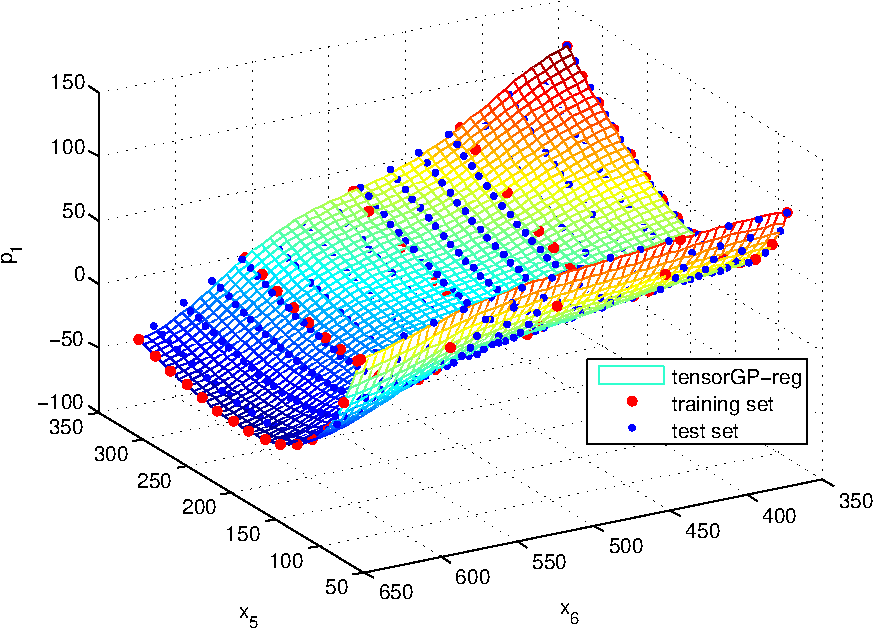
\includegraphics[width=\textwidth]{figures/gp_on_grid/rotating_disk_tensorGP.pdf}
      \caption{The proposed approach.}
      \label{fig:rotating_disc_tensorGP}
  \end{subfigure}
  \caption{2D slice along $x_5$ and $x_6$ variables (other variables are fixed) of tensorGP-reg approximation.}
\end{figure}

\section{Incomplete Factorial Design of Experiments}

A subset $\boldsymbol{\widetilde{\Omega}} \subseteq \boldsymbol{\Omega}$ of size
$\widetilde{N}$ of the full factorial DoE
is referred to as {\em incomplete factorial design of experiments}.
In general taking a subset of $\Omega$ breaks the structure of the dataset,
so we cannot apply the same techniques described in the previous section.
However, the partial structure that is preserved can be of use,
though at a higher computational cost.
We use the same notation for the trainig set in this section
$\mathcal{D} = \{(\mathbf{x}_i, y_i)\}_{i=1}^{\widetilde{N}}$.

\subsection{Log-likelihood and posterior distribution calculation}

To calculate the log-likelihood and the posterior mean we need to calculate
$\mathbf{K}_y^{-1}\mathbf{y}$ and the determinant $|\mathbf{K}_y|$.

Let $\mathbf{W}$ be a diagonal matrix of size $N \times N$,
where $N$ is the size of the full factorial DoE
$\boldsymbol{\widetilde{\Omega}} \supseteq \boldsymbol{\Omega}$.
Denote $R = N - \widetilde{N}$.
Let
$\mathbf{X} =
\{\mathbf{x}_i: \mathbf{x}_i \in \boldsymbol{\Omega}\}_{i = 1}^{N}$.
Then
\begin{equation*}
\mathbf{W}_{ii} =
\begin{cases}
    1, \mbox{ if } \mathbf{x}_i \in \boldsymbol{\Omega}, \\
    0, \mbox{ if } \mathbf{x}_i \notin \boldsymbol{\Omega}.
\end{cases}
\end{equation*}
We construct the vector $\mathbf{\widetilde{y}}$ as follows:
if $\mathbf{x}_i \in \boldsymbol{\widetilde{\Omega}}$,
then $\mathbf{\widetilde{y}}_i$ is filled with elements from $\mathbf{y}$
corresponding to $\mathbf{x}_i$.
The rest of the elements of $\mathbf{\widetilde{y}}$ we fill arbitrarily.
Now the matrix $\mathbf{\widetilde{K}}$ is the covariance matrix between points from
the set $\boldsymbol{\Omega}$.
Let us consider the following system of equations
\begin{equation}
\label{eq:incomplete_inverse}
\left (\mathbf{W \widetilde{K}} + \sigma^2_{noise}\mathbf{I} \right )\mathbf{z} =
\mathbf{W\widetilde{y}}.
\end{equation}
Notice, that equations that correspond to missing values
have the form $\sigma_{noise}^2 \mathbf{z}_j = 0$.
Therefore, the elements of $\mathbf{z}$ that correspond to missing values are equal to zero.
The other elements are solutions of the equation $\mathbf{K}_y \mathbf{z}' = \mathbf{y}$,
which gives us $\mathbf{K}_y^{-1}\mathbf{y}$.
To solve \eqref{eq:incomplete_inverse} we use conjuage gradients (CG) approach.
For CG the matrix should be symmetric, so let's multiply the left hand side and the right hand
side by
$\mathbf{\widetilde{K}}$:
\[
\left (\mathbf{\widetilde{K} W \widetilde{K}} + \sigma^2_{noise}\mathbf{\widetilde{K}} \right) \mathbf{z} =
\mathbf{\widetilde{K}}\mathbf{W\widetilde{y}}.
\]
By substituting $\mathbf{\widetilde{z}} = \mathbf{\sqrt{K} z}$ we obtain
a system with lower condition number:
\[
\left (\mathbf{\sqrt{\widetilde{K}} W \sqrt{\widetilde{K}}} + \sigma^2_{noise} \mathbf{I} \right )\mathbf{\widetilde{z}} =
\mathbf{\sqrt{\widetilde{K}} W \widetilde{y}},
\]
where $\mathbf{\sqrt{\widetilde{K}}} = \mathbf{U \sqrt{D} U}^T$, $\mathbf{U}$ --- is a
matrix of eigenvectors of
$\mathbf{\widetilde{K}}$,
$\mathbf{D}$ --- is a diagonal matrix with eigenvalues of $\mathbf{\widetilde{K}}$.
Note, that fast matrix-vector products can be calculated by using the results of
the section \ref{sec:calc_loglikelihood}.

It is well known that CG converges at most in $r$ iterations, where
$r$ is a number of different eigenvalues of the system matrix \cite{nocedal2006numerical}.
In the system that we obtained we can do such change of variables,
that the number of different eigenvalues is equal to either $R + 1$ or $\widetilde{N} + 1$:
\begin{enumerate}
\item Change of variables 1:
\[
\mathbf{z}_1 = \sqrt{\mathbf{\widehat{D}}} \mathbf{U}^T \mathbf{\widetilde{z}},
\]
where $\mathbf{\widehat{D}} = \mathbf{D} + \sigma^2_{noise}\mathbf{I}$.
The system of equations in this case looks like
\begin{equation}
\label{eq:variables_change_1}
        \left ( \sqrt{\mathbf{\widehat{D}}^{-1} \mathbf{D}} \mathbf{U}^T (\mathbf{W - I})
            \mathbf{U}\sqrt{\mathbf{D \widehat{D}}^{-1}} + \mathbf{I}
        \right ) \mathbf{z}_1 = \sqrt{\mathbf{\widehat{D}}^{-1} \mathbf{D}} \mathbf{U}^T \mathbf{W \widetilde{y}}.
\end{equation}
\item Change of variables 2:
\[
\mathbf{z}_2 = \mathbf{U}^T \mathbf{\widetilde{z}}.
\]
In this case we obtain:
\begin{equation}
\label{eq:variables_change_2}
        \left ( \sqrt{\mathbf{D}} \mathbf{U}^T \mathbf{W}
            \mathbf{U}\sqrt{\mathbf{D}} + \sigma^2_{noise}\mathbf{I}
        \right ) \mathbf{z}_2 = \sqrt{\mathbf{D}} \mathbf{U}^T \mathbf{W \widetilde{y}}.
\end{equation}
\end{enumerate}

\begin{proposition}
The matrix of the system of equations \eqref{eq:variables_change_1} has no more than $R + 1$
different eighevalues,
while the matrix \eqref{eq:variables_change_2} has no more than $\widetilde{N} + 1$.
\end{proposition}
\begin{proof}
    Let us show the proof for \eqref{eq:variables_change_2}.
    The statement for \eqref{eq:variables_change_1} can be proved similarly.
    The rank of matrix $\mathbf{W}$ is equal to $\widetilde{N}$.
    As the rank of the product of matrices is not greater than the rank of the factors,
    the rank of the matrix
    $\mathbf{A} = \sqrt{\mathbf{D}} \mathbf{U}^T \mathbf{W} \mathbf{U}\sqrt{\mathbf{D}}$
    is not greater than $\widetilde{N}$.
    Now, the matrix $\mathbf{A}$ is symmetric and has $N$ real eigenvalues
    $\lambda_i, i = 1, \ldots, N$.
    Moreover, as the rank is not greater than $\widetilde{N}$, than the number of different eigenvalues
    is not greater than $\widetilde{N}$ too.
    The eigenvalues of the matrix in \eqref{eq:variables_change_2}
    are equal to $\lambda_i + \sigma^2_{noise}$.
    Hence, the matrix has no more than $\widetilde{N} + 1$ different eigenvalues.
\end{proof}


The computational complexity of one iteration of CG as the same as the complexity
of computing $\mathbf{\widetilde{K}}_y \mathbf{x}$,
therefore, the overall complexity of computing $\mathbf{K}_y^{-1}\mathbf{y}$ is
\[
\mathcal{O}\left (\min\{R + 1, \widetilde{N} + 1\} N\sum_{i = 1}^K n_i \right ).
\]
Assuming,
that $n_i \ll N$ (i.e. the number of factors is large, and their sizes are equal),
we obtain
$\mathcal{O}(\min\{R + 1, \widetilde{N} + 1\} N^{1 + \frac{1}{K}})$.
So, if less than half of points is missing the complexity is linear in number of missing poitns.
$\mathcal{O}((R + 1)N^{1 + \frac{1}{K}})$.
In the limit when there are no missing points the complexity is the same
as the complexity for full factorial DoE.


\subsection{Calculation of the determinant}
Let $\mathbf{A}$ be a covariance matrix of size $N \times R$ between training points and
missing points,
and $\mathbf{B}$ be a covariance matrix of size $R \times R$ between missing points.
Then matrix $\mathbf{\widetilde{K}}_y$ can be represented as a block matrix
\[
\mathbf{\widetilde{K}_y} = \begin{pmatrix}
  \mathbf{K}_y & \mathbf{A} \\
  \mathbf{A}^T & \mathbf{B}
\end{pmatrix}.
\]
The determinant of the block matrix can be calculated as follows
$|\mathbf{\widetilde{K}}_y | = |\mathbf{K}_y| |\mathbf{B} - \mathbf{A}^T \mathbf{K}_y^{-1}\mathbf{A}|$,
therefore, the determinant of interest is given by
\begin{equation}
\label{eq:determinant_incomplete}
|\mathbf{K}_y| = \frac{|\mathbf{\widetilde{K}}_y |}{|\mathbf{B} - \mathbf{A}^T \mathbf{K}_y^{-1}\mathbf{A}|}.
\end{equation}
The computational complexity of this expression is
$\mathcal{O}(\min\{R + 1, \widetilde{N} + 1\} R N\sum_{i = 1}^K n_i)$,
because we need to calculate matrix-vector multiplication $\mathbf{K}_y^{-1}\mathbf{A}_i$
$R$ times,
where $\mathbf{A}_i$ is an $i$-th column of matrix $\mathbf{A}$.
The memory complexity equals $\mathcal{O}(R\widetilde{N} + N + \sum_{i = 1}^K n_i^2)$.

However, we can reduce memory to $\mathcal{O}(\widetilde{N})$ and improve the constant in complexity of
\eqref{eq:determinant_incomplete}.
For this, notice that the approach to calculate $\mathbf{K}_y^{-1}\mathbf{y}$
also allows to calculate $\mathbf{C}^{-1}\mathbf{v}$,
where $\mathbf{C}$ is an arbitrary principal submatrix of size $m \times m$
of the matrix $\mathbf{\widetilde{K}}_y$,
and $\mathbf{v}$ is any vector of length $m$.
The computational complexity of the operation in this case is
$\mathcal{O} \left (\min\{m + 1, \widetilde{N} - m + 1\}
\widetilde{N}\sum_{i = 1}^K n_i \right )$.

Denote
\[
\mathbf{\widetilde{K}}_y = \begin{pmatrix}
  \mathbf{K}_1 & \mathbf{a}_1 \\
  \mathbf{a}_1^T & b_1
\end{pmatrix},
\]
where $\mathbf{K}_1$ is of size $(\widetilde{N} - 1) \times (\widetilde{N} - 1)$,
$\mathbf{a}_1$ is a vector of length $\widetilde{N} - 1$, $b_1$ is a scalar.
Then
\[
|\mathbf{\widetilde{K}}_y| = |\mathbf{K}_1| (b_1 - \mathbf{a}_1^T \mathbf{K}_1^{-1}\mathbf{a}_1).
\]
Similarly, splitting $\mathbf{K}_1$ into blocks
$\begin{pmatrix}
\mathbf{K}_2 & \mathbf{a}_2 \\
\mathbf{a}_2 & b_2
\end{pmatrix}$,
and splitting matrix $\mathbf{K}_2$ into
$\begin{pmatrix}
\mathbf{K}_3 & \mathbf{a}_3 \\
\mathbf{a}_3 & b_3
\end{pmatrix}$,
and so on, we obtain
\[
|\mathbf{\widetilde{K}}_y| =
|\mathbf{K}_y| \prod_{i = 1}^R(b_i - \mathbf{a}_i^T\mathbf{K}_i^{-1}\mathbf{a}_i),
\]
or
\begin{equation}
\label{eq:determinant_incomplete_practical}
|\mathbf{K}_y| =
\frac{|\mathbf{\widetilde{K}}_y|}{\prod_{i = 1}^R(b_i -
\mathbf{a}_i^T\mathbf{K}_i^{-1} \mathbf{a}_i)}.
\end{equation}
Here to calculate the right hand side we need to store only $\mathbf{K}_i^{-1}\mathbf{a}_i$,
therefore, the total memory complexity is $\mathcal{O}(N + \sum_{i = 1}^K n_i^2)$.

The complexity of calculation of each $\mathbf{K}_i^{-1}\mathbf{a}_i$ is lower
than the complexity of calculation of $\mathbf{K}_y^{-1}\mathbf{A}_i$,
thus, the expression \eqref{eq:determinant_incomplete_practical} is more efficient,
although asymptotically it is the same.


\subsection{Experiments}
To compare the classical approach for GP regression against the proposed approach
we generated several datasets with incomplete factorial DoE.
The dimensionality of input is $5$, factor sizes are equal to $[5, 4, 4, 4, 4]$, the number of missing points varies from $100$ to $320$.
In \fig{time_itgp} you can see the ratio of computation time of the standard approach (GP)
and the training time of the proposed approach (iTensorGP) for different number of missing
values.
Theory shows that the ratio should be $\frac{(N - R)^3}{R^2 N(\sum_{i = 1}^K n_i)}$.
Then the number of missing points increases, so does the training time of iTensorGP.
At some points iTensorGP becomes less efficient than the standard GP approach.
However, in case of a small amount of missing points iTensorGP is much faster.

\begin{figure}
  \centering
  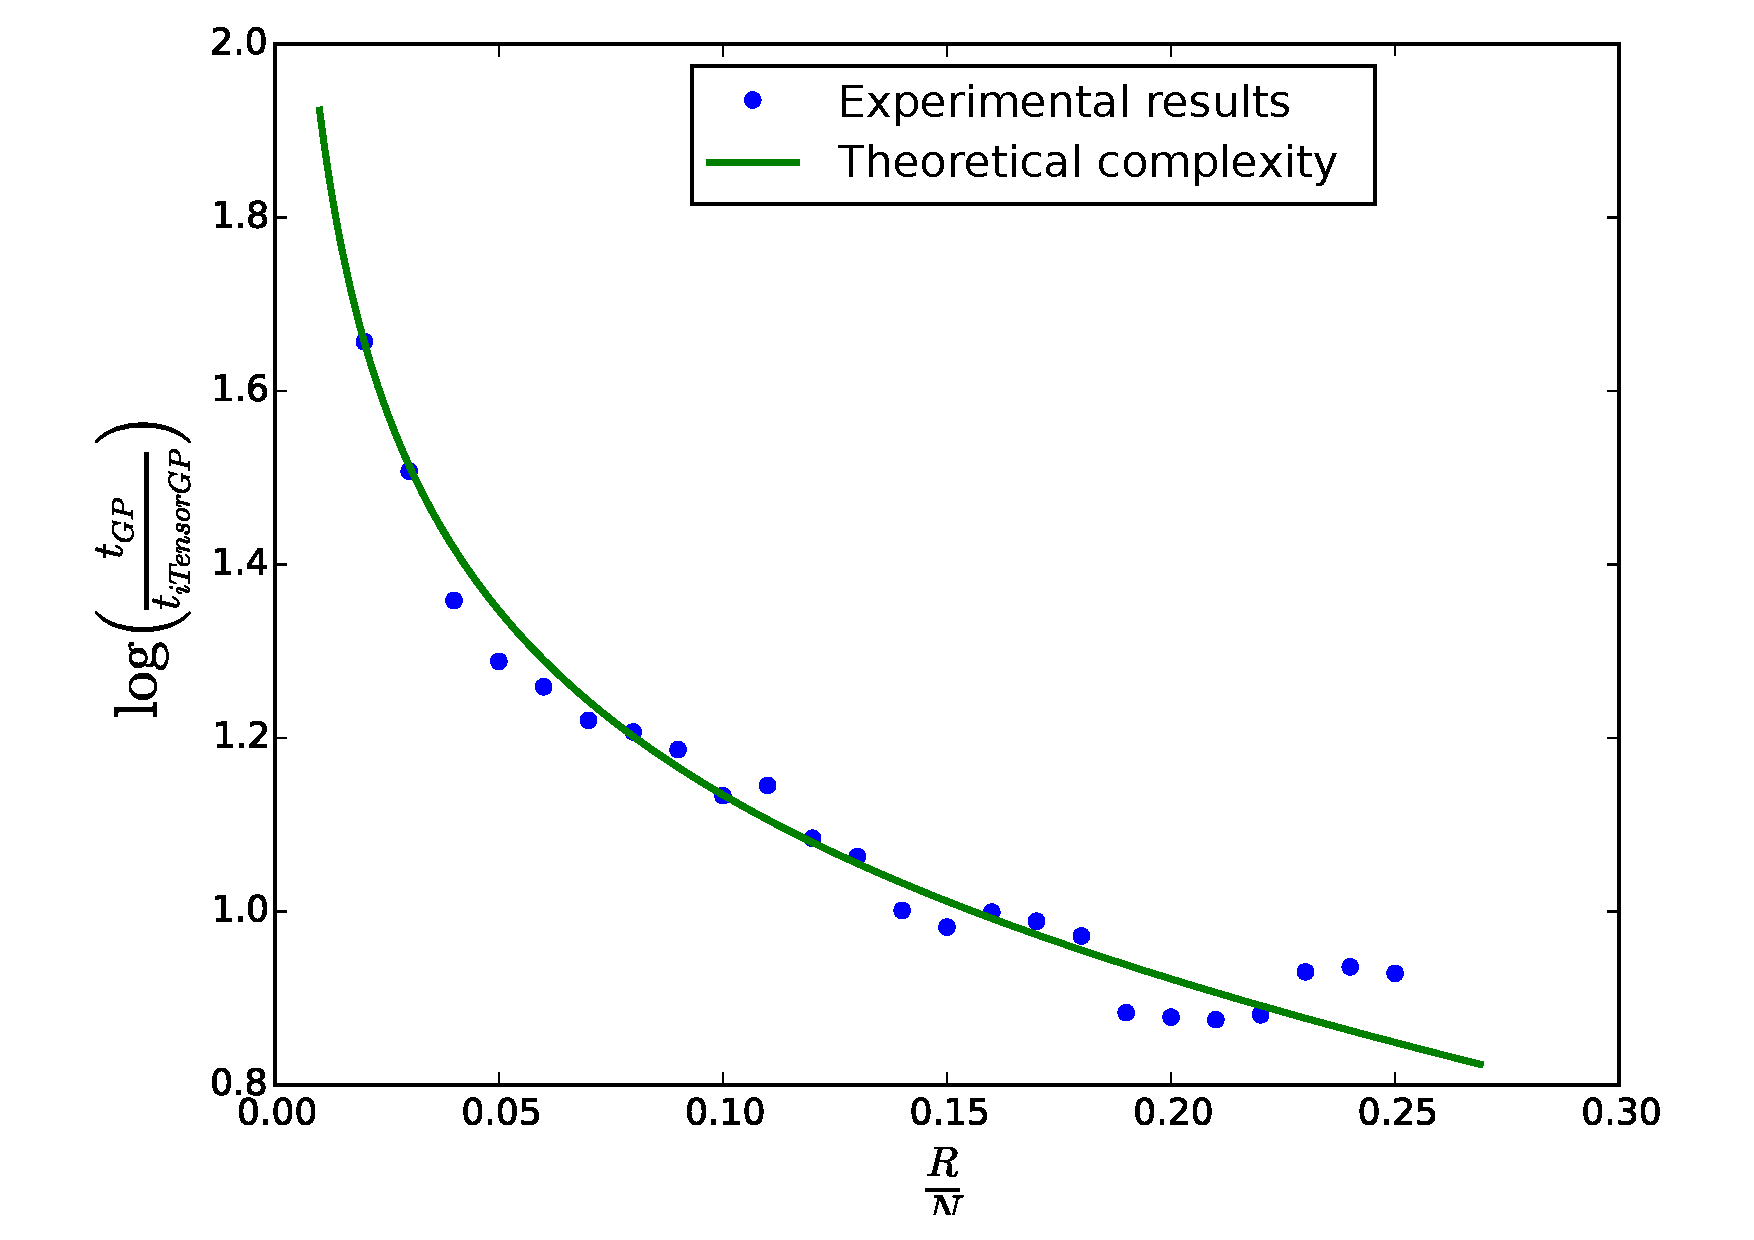
\includegraphics[width=0.5\textwidth]{figures/incomplete_grid/time_comparison_itgp.pdf}
  \caption{Comparison of the training time of the proposed approach (iTensorGP) and
  standard approach (GP).}
  \label{fig:time_itgp}
\end{figure}




\chapter{Large-Scale Kernel Methods for Unstructured Datasets}
\label{chap:unstructured_datasets}
In vast majority of real-world problems the data sets do not have the factorial structure.
In this case the are several approaches to scale up the GP model.
One way is to aggregate several smaller models into big one,
e.g. Mixture of GPs and Bayesian Machine Committee
\citep{rasmussen2006gaussian, rasmussen2001infinite}.
The idea here is to split data set into several smaller subsets
$\mathcal{D}_i, i=1, \ldots, M$, build on each data set GP model and then combine them.
In Bayesian committee machine, for example, the final distribution is given by
\[
    p(y^* | \mathcal{D}) \sim \frac{\prod_{i=1}^M p(y^* | \mathcal{D}_i)}{p(y^*)},
\]
supposeing that the correlation between subsets is small.

Another class of methods builds lightweight approximation of the kernel function.
There are data dependent approaches that follow Nystr{\"o}m's method for kernel approximation
\citep{rasmussen2006gaussian}.
The idea of approximation is based on numerical approximation of the {\em eigenfunctions}
and {\em eigenvalues} of the kernel function.
A function $\phi(\cdot)$ that satisfies the following equation
\[
    \int k(\mathbf{x, x}')\phi(\mathbf{x}) d\mu(\mathbf{x}) = \lambda \phi(\mathbf{x}')
\]
is called eigenfunction of kernel $k$, $\lambda$ is a corresponding eigenvalue
with respect to measure $\mu$.
If we let $d\mu(\mathbf{x}) = p(\mathbf{x})d\mathbf{x}$ we can write down
numerical approximation to the equation
\begin{equation}
\label{eq:eigenfunction_approx}
    \lambda_i \phi_i(\mathbf{x}) \simeq
    \frac{1}{M} \sum_{k=1}^M k(\mathbf{x}_k, \mathbf{x}) \phi_i(\mathbf{x}_k),
\end{equation}
where points $\mathbf{x}_k$ are generated from distribution $p(\mathbf{x})$
and called {\em inducing points}.
By plugging $\mathbf{x}_i$ from the training set into equation above we obtain
\[
    \mathbf{K}_f \mathbf{u}_i = \hat{\lambda}_i \mathbf{u}_i,
    \quad
    \phi_i(\mathbf{x}_j) = \sqrt{\hat{\lambda}_i} \left ( \mathbf{u}_i \right )_j.
\]
And now from \eqref{eq:eigenfunction_approx} we obtain {\em Nystr{\"o}m} approximation
of the $i$-th eigenfunction $\phi(\mathbf{x}) = \frac{M}{\hat{\lambda}_i}\mathbf{k}^\T \mathbf{u}_i$, and, therefore, approximation of the kernel matrix
\begin{equation}
\label{eq:nystrom_matrix}
    \mathbf{K}_f \simeq \widehat{\mathbf{K}}_f = \mathbf{K}_{NM}\mathbf{K}_{MM}^{-1}\mathbf{K}_{MN},
\end{equation}
where $\mathbf{K}_{MN}$ is a covariance matrix between training points and inducing points
and $\mathbf{K}_{MM}$ is a covariance between inducing points.
More details can be found in \citep{rasmussen2006gaussian}.

In \citep{williams2001using} the authors first proposed to use
\eqref{eq:nystrom_matrix} approximation in posterior distribution of GP regression model.
The computational complexity is reduced to $\mathcal{O}(NM^2 + M^3)$ operations
which gives benefit if $M \ll N$.
There are several works that build on top of Nystr{\"o}m approximation trying to refine
the approximation of the covariance matrix and, thus, improve the quality of the model
while preserving low computational complexity \citep{quinonero2005unifying, rossi2020sparse}.

In this thesis we consider different type of approximations based on so called
{\em random features}.
The idea of the approach is to construct approximation of the kernel function
that enables low-rank approximation of the kernel matrix.
To construct such approximation we need to consider the kernel function from different
perspective.
It turns out that every positive definite kernel $k$ uniquely defines some space of functions
and vice versa.
Moreover, it can be seen as an inner products in an appropriate Hilbert space.

\begin{definition}[Positive definite kernels]
    Let $\mathcal{X}$ be a nonempty set.
    A symmetric function $k \colon \mathcal{X} \times \mathcal{X} \rightarrow \mathbb{R}$
    is called a positive definite kernel, if for any set $\mathbf{x}_1, \ldots, \mathbf{x}_N$,
    $\forall N \in \mathbb{N}$ and for any $(c_1, \ldots, c_N)\subset \mathbb{R}$ it holds
    \[
        \sum_{i=1}^N \sum_{j=1}^N c_i c_j k(\mathbf{x}_i, \mathbf{x}_j) \geq 0.
    \]
\end{definition}

Note, that the covariance function that we use in GP are also positive definite kernels.

\begin{definition}[RKHS, \citep{aronszajn1950theory}]
Let $\mathcal{X}$ be a nonempty set and $k$ be a positive definite kernel on $\mathcal{X}$.
A Hilbert space $\mathcal{H}$ of function on $\mathcal{X}$ with an inner-product
$\langle \cdot, \cdot \rangle_{\mathcal{H}}$ is called a reproducing kernel
Hilbert space (RKHS) with reproducing kernel $k$, if the following is satisfied
    \begin{enumerate}
        \item For all $\mathbf{x} \in \mathcal{X}$ we have
        $k(\cdot, \mathbf{x}) \in \mathcal{H}$;
        \item for all $\mathbf{x} \in \mathcal{X}$ and for all $f\in \mathcal{H}$
        \[
            f(\mathbf{x}) = \langle f, k(\cdot, \mathbf{x}) \rangle
            \tag*{Reproducing property}.
        \]
    \end{enumerate}
\end{definition}
In reproducing property we used $k(\cdot, \mathbf{x})$ which is actually
a real-valued function such that $\mathbf{y} \rightarrow k(\mathbf{y, x})$
for $\forall \mathbf{y} \in \mathcal{X}$.
So, the kernel function satisfies
\[
    k(\mathbf{x, y}) = \langle k(\cdot, \mathbf{x}), k(\cdot, \mathbf{y}) \rangle,
    \quad \mathbf{x, y} \in \mathcal{X}.
\]
$k(\cdot, \mathbf{x})$ is called {\em canonical feature map} of $\mathbf{x}$.
There can be a lot of different features maps
$\psi \colon \mathcal{X} \rightarrow \mathcal{H}$ such that their inner product is defined
by the kernel function $k(\mathbf{x, y}) = \langle \psi(\mathbf{x}), \psi(\mathbf{y})$.

The idea for kernel approximation using randomized feature map is based
on finding finite-dimensional maps that approximate the inner-product that is associated
with the kernel function.

The main contributions of this chapter are as follows.
\begin{itemize}
    \item We introduce a technique for kernel approximation based on randomzied feature maps
    and special quadrature rules.
    \item We derive error bounds for the developed approach.
    \item We show that \citep{rahimi2008random,felix2016orthogonal} are special cases of the
    proposed method.
\end{itemize}




\section{Quadrature-based Features for Kernel Approximation}

\subsection{Random Fourier Features}
\label{sec:random_fourier_features}
One of the most well-known approach is called
Random Fourier Features (RFF).
It was first proposed by \citep{rahimi2008random}, and it is based on Bochner's theorem.
\begin{theorem}[Bochner]
    A continuous kernel $k(\mathbf{x, x'}) = k(\mathbf{r}), \mathbf{r = x - x'}$ on
    $\mathbb{R}^d$ is positive definite if and only if
    $k(\mathbf{r})$ is a Fourier transform of a non-negative measure $p(\mathbf{w})$
    \begin{equation}
    \label{eq:bochner}
        k(\mathbf{r}) = \int_{\Omega} p(\mathbf{w}) e^{j\mathbf{w^{\T}(x - x')}} d\mathbf{w}.
    \end{equation}
\end{theorem}
By applying Monte-Carlo sampling to approximate integral in~\eqref{eq:bochner}
RFF introduces a low-dimensional randomized approximation to feature maps:
\begin{equation}
\label{eq:inner}
    k(\mathbf{x, y}) \approx
    \mathbf{\hat{\Psi}}(\mathbf{x})^{\boldsymbol{\top}} \mathbf{\hat{\Psi}}(\mathbf{y}),
\end{equation}
\[
    \mathbf{\hat{\Psi}}(\mathbf{x}) =
    \frac{1}{\sqrt{D}} \begin{bmatrix}
        \cos(\mathbf{w}_1^\T\mathbf{x}) \\
        \sin(\mathbf{w}_1^\T \mathbf{x}) \\
        \cdots \\
        \cos(\mathbf{w}_D^\T \mathbf{x}) \\
        \sin(\mathbf{w}_D^\T \mathbf{x}) \\
    \end{bmatrix}, \quad \mathbf{w}_i \sim p(\mathbf{w}),
\]
where $D$ is a number of generated samples.
Exploiting the idea with an integral representation of the dot product
\[
k(\mathbf{x, y}) = \int_{\Omega} \psi(\mathbf{w, x}) \psi(\mathbf{w, y}) p(\mathbf{w}) d\mathbf{w},
\]
we can construct low-rank approximations to a wider class of kernel functions
(not only shift-invariant kernels).
In this case the feature map $\mathbf{\hat{\Psi}}(\mathbf{x})$ looks like
\[
    \mathbf{\hat{\Psi}}(\mathbf{x}) = \frac{1}{\sqrt{D}} \begin{bmatrix}
        \psi(\mathbf{w}_1, \mathbf{x}) \\
        \cdots \\
        \psi(\mathbf{w}_D, \mathbf{x})
    \end{bmatrix},
    \quad
    \mathbf{w} \sim p(\mathbf{w}).
\]








A randomized $D$-dimensional mapping $\mathbf{\hat{\Psi}}(\cdot)$ applied to the original data
input allows employing standard linear methods, i.e. reverting the kernel trick. In doing so
one reduces the complexity to that of linear methods, e.g. $D$-dimensional approximation
admits $\mathcal{O}(ND^2)$ training time, $\mathcal{O}(ND)$ memory and  $\mathcal{O}(N)$
prediction time.

It is well known from the theory on Monte Carlo based estimates
that as $D \rightarrow \infty$, the randomized feature maps based
approximations converge to the exact kernel $k(\mathbf{x, y})$.
Recent research \citep{yang2014quasi, felix2016orthogonal, choromanski2016recycling} aims to improve the convergence of approximation so that a smaller $D$ can be used to obtain the same quality of approximation.

Here we will consider the class of kernels admitting the following integral representation
\begin{equation}
\label{eq:integral_representation}
    \begin{aligned}
        k(\mathbf{x}, \mathbf{y}) =
        \mathbb{E}_{p(\mathbf{w})} f_{\mathbf{xy}}(\mathbf{w}) =
        I(f_{\mathbf{xy}}),
        \quad p(\mathbf{w}) = \frac{1}{(2 \pi)^{d/2}} e^{-\frac{\|\mathbf{w}\|^2}{2}},
        \\
        \quad f_{\mathbf{xy}} = \phi(\mathbf{w}^{\T}\mathbf{x})
        \phi(\mathbf{w}^{\T} \mathbf{y}).
    \end{aligned}
\end{equation}
It includes the class of shift-invariant kernels,
e.g. the popular Gaussian kernel with
$f_{\mathbf{xy}}(\mathbf{w}) =
\phi(\mathbf{w}^{\boldsymbol{\top}}\mathbf{x})^{\boldsymbol{\top}}
\phi(\mathbf{w}^{\boldsymbol{\top}}\mathbf{y})$,
where $\phi(\cdot) = \begin{bmatrix}\cos(\cdot) & \sin(\cdot) \end{bmatrix}^{\boldsymbol{\top}}$.
It also contains Pointwise Nonlinear Gaussian (PNG) kernels.
They are widely used in practice and have interesting connections with neural networks
\citep{cho2009kernel, williams1997computing}.

The main challenge for the construction of low-dimensional feature maps is the approximation of the expectation in \eqref{eq:integral_representation} which is $d$-dimensional integral with Gaussian weight.
To improve the approximation we introduce quarature rules to approximate the integral
and then show that they generalize several prominent papers in this topic.
% Unlike other research studies we refrain from using simple Monte Carlo estimate of the integral, instead, we propose to use specific quadrature rules.
% We now list our contributions:
% \begin{itemize}
% \item We propose to use spherical-radial quadrature rules to improve kernel approximation accuracy.
% We show that these quadrature rules generalize the RFF-based techniques.
% We also provide an analytical estimate of the error for the used quadrature rules that implies better approximation quality.
% \item
% We use structured orthogonal matrices (so-called \emph{butterfly matrices}) when designing quadrature rule that allow fast
% matrix by vector multiplications.
% As a result, we speed up the approximation of the kernel function and reduce memory requirements.
% \item
% We carry out an extensive empirical study comparing our methods with the state-of-the-art ones on a set of different kernels in terms of both kernel approximation error and downstream tasks performance. The study supports our hypothesis on the exceeding accuracy of the method.
% \end{itemize}


\section{Quadrature Rules}
\label{sec:quadrature_rule}
We start with rewriting the expectation in Equation \eqref{eq:integral_representation} as integral of $f_{\mathbf{xy}}$ with respect to $p(\mathbf{w})$:
\begin{equation*}
I(f_{\mathbf{xy}}) = (2\pi)^{-\frac{d}{2}} \int_{-\infty}^{\infty} \dots  \int_{-\infty}^{\infty} e^{-\frac{\mathbf{w}^{\boldsymbol{\top}}\mathbf{w}}{2}} f_{\mathbf{xy}}(\mathbf{w})d\mathbf{w}.
\end{equation*}
Integration can be performed by means of quadrature rules. The rules usually take a form of interpolating function that is easy to integrate. Given such a rule, one may sample points from the domain of integration and calculate the value of the rule at these points. Then, the sample average of the rule values would yield the approximation of the integral.

The connection between integral approximation and mapping $\psi$ is straightforward. In what follows we show a brief derivation of the quadrature rules that allow for an explicit mapping of the form:
${
    \psi(\mathbf{x}) = [\enskip a_0 \phi(0) \enskip
    a_1 \phi(\mathbf{w}_1^{\top} \mathbf{x})
    \enskip \dots \enskip
    a_D \phi(\mathbf{w}_{D}^\top \mathbf{x}) \enskip],}
$
where the choice of the weights $a_i$ and the points $\mathbf{w}_i$ is dictated by the quadrature.

We use the average of sampled quadrature rules developed by \citep{genz1998stochastic} to yield unbiased estimates of $I(f_{\mathbf{xy}})$. A change of coordinates is the first step to facilitate stochastic spherical-radial rules. Now, let $\mathbf{w} = r\mathbf{z}$, with $\mathbf{z}^{\boldsymbol{\top}}\mathbf{z} = 1$, so that $\mathbf{w}^{\boldsymbol{\top}}\mathbf{w}=r^2$ for $r \in [0, \infty]$, leaving us with (to ease the notation we substitute $f_{\mathbf{xy}}$ with $f$)
\begin{equation}
\begin{split}
\label{eq:polar}
I(f) = (2\pi)^{-\frac{d}{2}} \int_{U_d} \int_{0}^{\infty} e^{-\frac{r^2}{2}} r^{d-1} f(r\mathbf{z})dr d\mathbf{z} =
\frac{(2\pi)^{-\frac{d}{2}}}{2} \int_{U_d} \int_{-\infty}^{\infty} e^{-\frac{r^2}{2}} |r|^{d-1} f(r\mathbf{z})dr d\mathbf{z},
\end{split}
\end{equation}
$I(f)$ is now a double integral over the unit $d$-sphere $U_d = \{\mathbf{z}: \mathbf{z}^{\boldsymbol{\top}}\mathbf{z} = 1, \mathbf{z} \in \mathbb{R}^d\}$ and over the radius. To account for both integration regions we apply a combination of spherical ($S$) and radial ($R$) rules known as spherical-radial ($SR$) rules.
To provide an intuition how the rules work, here we briefly state and discuss their form.

\textbf{Stochastic radial rules} of degree ${2l+1}$
$R(h) = \sum\limits_{i=0}^{l} \hat{w}_i \frac{h(\rho_i) + h(-\rho_i)}{2}$
have the form of the weighted symmetric sums and approximate the infinite range integral
$T(h) = \int_{-\infty}^{\infty} e^{-\frac{r^2}{2}} |r|^{d-1} h(r) dr$.
Note that when $h$ is set to the function $f$ of interest, $T(f)$ corresponds to the inner integral in \eqref{eq:polar}.
To get an unbiased estimate for $T(h)$, points $\rho_i$ are sampled from specific distributions.
The weights $\hat{w}_i$ are derived so that the rule is exact for
polynomials of degree $2l + 1$ and give unbiased estimate for other functions.

\textbf{Stochastic spherical rules} ${S_\mathbf{Q}(s) = \sum\limits_{j=1}^{p} \widetilde{w}_j s(\mathbf{Qz}_j),}$ where
$\mathbf{Q}$ is a random orthogonal matrix, approximate an integral of a function $s(\mathbf{z})$ over the surface of unit $d$-sphere $U_d$,
where $\mathbf{z}_j$ are points on $U_d$, i.e. $\mathbf{z}_j^{\boldsymbol{\top}}\mathbf{z}_j = 1$. Remember that the outer integral in \eqref{eq:polar} has $U_d$ as its integration region.
The weights $\widetilde{w}_j$ are stochastic with distribution such that
the rule is exact for polynomials of degree $p$ and gives unbiased estimate
for other functions.

\textbf{Stochastic spherical-radial rules} $SR$ of degree $(2l + 1, p)$ are given by the following expression\footnote{Please see \citep{genz1998stochastic} for detailed derivation of SR rules.}
\[
SR^{(2l + 2, p)}_{\mathbf{Q}, \rho} = \sum_{j = 1}^p \widetilde{w}_j
\sum_{i = 1}^{l} \hat{w}_i \frac{f(\rho\mathbf{Qz}_i) + f(-\rho \mathbf{Qz}_i)}{2},
\]
where the distributions of weights are such that if degrees of radial
rules and spherical rules coincide, i.e. $2l + 1 = p$, then the rule is exact
for polynomials of degree $2l + 1$ and gives unbiased estimate of the integral for other functions.

\subsection{Spherical-radial rules of degree (1, 1)}
\begin{proposition}
Random Fourier Features for RBF kernel are SR rules of degree~$(1, 1)$.
\end{proposition}
\begin{proof}
    If we take radial rule of degree $1$ and spherical rule of degree $1$,
    we obtain the following rule
    $SR^{(1, 1)}_{\mathbf{Q}, \rho} = \frac{f(\rho \mathbf{Qz}) + f(-\rho\mathbf{Qz})}{2},$
    where $\rho \sim \chi(d)$.
    It is easy to see that ${\rho \mathbf{Qz} \sim \mathcal{N}(0, \mathbf{I})}$,
    and for shift invariant kernel ${f(\mathbf{w}) = f(-\mathbf{w})}$, thus, the rule reduces
    to
    ${SR^{(1, 1)}_{\mathbf{Q}, \rho} =
    f(\mathbf{w})}$, where ${\mathbf{w} \sim \mathcal{N}(0, \mathbf{I}).}$
    Now, RFF \citep{rahimi2008random} makes approximation
    of the RBF kernel in exactly the same way: it generates random vector from Gaussian
    distribution and calculates the corresponding feature map.
\end{proof}



\subsection{Spherical-radial rules of degree (1, 3)}
\begin{proposition}
Orthogonal Random Features for RBF kernel are SR rules of degree~$(1, 3)$.
\end{proposition}
\begin{proof}
    Let us take radial rule of degree 1 and spherical rule of degree 3.
    In this case we get the following spherical-radial rule
    ${SR^{1, 3}_{\mathbf{Q}, \rho} = \sum_{i = 1}^d
    \frac{f(\rho\mathbf{Qe}_i) + f(-\rho\mathbf{Qe}_i)}{2},}$
    where ${\rho \sim \chi(d)}$,
    ${\mathbf{e}_i = (0, \ldots, 0, 1, 0, \ldots, 0)^{\boldsymbol{\top}}}$
    is an $i$-th column of the identity matrix.

    Let us compare $\text{SR}^{1,3}$ rules with Orthogonal Random Features \citep{felix2016orthogonal} for the RBF kernel.
    In the ORF approach, the weight matrix $\mathbf{W} = \mathbf{SQ}$ is generated, where $\mathbf{S}$ is a diagonal matrix with the entries drawn independently from $\chi(d)$ distribution and $\mathbf{Q}$ is a random orthogonal matrix.
    The approximation of the kernel is then given by
    $k_{\text{ORF}}(\mathbf{x}, \mathbf{y}) = \sum_{i = 1}^d f(\mathbf{w}_i)$, where $\mathbf{w}_i$ is the $i$-th row of the matrix $\mathbf{W}$.
    As the rows of $\mathbf{Q}$ are orthonormal, they can be represented as $\mathbf{Qe}_i$.
\end{proof}


\subsection{Spherical-radial rules of degree (3, 3)}
We go further and take both spherical and radial rules of degree 3, where we use original and reflected vertices $\mathbf{v}_j$ of randomly rotated unit vertex regular $d$-simplex $\mathbf{V}$ as the points on the unit sphere
\begin{equation}
\begin{split}
\label{eq:sr33}
SR^{3,3}_{\mathbf{Q}, \rho}(f) = &\left (1 - \frac{d}{\rho^2} \right )f(\mathbf{0}) + \frac{d}{d+1}\sum\limits_{j=1}^{d+1} \left[ \frac{f(-\rho \mathbf{Qv}_j) + f(\rho \mathbf{Qv}_j)}{2\rho^2} \right],
\end{split}
\end{equation}
where  ${\rho \sim \chi(d+2)}$. We apply \eqref{eq:sr33} to the approximation of \eqref{eq:polar}
by averaging the samples of $SR^{3,3}_{\mathbf{Q}, \rho}$:
\begin{equation}
\begin{split}
\label{eq:estimate}
    I(f) = \mathbb{E}_{\mathbf{Q}, \rho} \lbrack SR^{3,3}_{\mathbf{Q},\rho}(f) \rbrack \approx \hat{I}(f) = \frac{1}{n}\sum\limits_{i=1}^{n} SR^{3,3}_{\mathbf{Q}_i,\rho_i}(f),
\end{split}
\end{equation}
where $n$ is the number of sampled $SR$ rules. Speaking in terms of the approximate feature maps, the new feature dimension $D$ in case of the quadrature based approximation equals $2n(d+1) + 1$ as we sample $n$ rules and evaluate each of them at $2(d+1)$ random points and $1$ zero point.

We propose to modify the quadrature rule by generating $\rho_j \sim \chi(d + 2)$ for each $\mathbf{v}_j$, i.e.
$SR^{3,3}_{\mathbf{Q}, \rho}(f) = \left (1 - \sum_{j = 1}^{d + 1}\frac{d}{(d + 1)\rho_j^2} \right )f(\mathbf{0}) + \frac{d}{d+1}\sum\limits_{j=1}^{d+1} \left[ \frac{f(-\rho_j \mathbf{Qv}_j) + f(\rho_j \mathbf{Qv}_j)}{2\rho_j^2} \right].$
It doesn't affect the quality of approximation while simplifies an analysis
of the quadrature-based random features.

\paragraph*{Explicit mapping} We finally arrive at the map
$\psi(\mathbf{x}) = \begin{bmatrix} a_0 \phi(0) &
    a_1 \phi(\mathbf{w}_1^{\top} \mathbf{x})
    & \dots &
    a_D \phi(\mathbf{w}_{D}^\top \mathbf{x}) \end{bmatrix},$
where $a_0 = \sqrt{1 - \sum\limits_{d+1}^{j=1}\frac{d}{\rho^2}}$
\footnote{To get ${a_0^2 \geq 0}$, you need to sample $\rho_j$ two times on average (see Appendix for details).},
%\todo{Move proof in main body}
$a_j = \frac{1}{\rho_j}\sqrt{\frac{d}{2(d + 1)}}$, $\mathbf{w}_j$ is the $j$-th row in the matrix ${\mathbf{W} = \boldsymbol{\rho} \otimes \Big[\begin{smallmatrix} & (\mathbf{QV}) ^\top \\
- & (\mathbf{QV})^\top \end{smallmatrix}\Big]}$, ${\boldsymbol{\rho} = [ \rho_1 \dots \rho_D ]^{\top}}$.
To get $D$ features one simply stacks $n = \frac{D}{2(d+1)+1}$ such matrices
$\mathbf{W}^k = \boldsymbol{\rho}^k\Big[\begin{smallmatrix} & (\mathbf{Q}^k\mathbf{V})^\top \\
- & (\mathbf{Q}^k\mathbf{V})^\top \end{smallmatrix}\Big]$
so that $\mathbf{W} \in \mathbb{R}^{D \times d}$, where only $\mathbf{Q}^k \in \mathbb{R}^{d \times d}$ and ${\boldsymbol{\rho}^k}$ are generated randomly $(k=1,\dots, n)$.
For Gaussian kernel, $\phi(\cdot) = \begin{bmatrix}\cos(\cdot) & \sin(\cdot) \end{bmatrix}^{\boldsymbol{\top}}$.
For the 0-order arc-cosine kernel, ${\phi(\cdot) = \Theta(\cdot)}$, where $\Theta(\cdot)$ is the Heaviside function.
For the 1-order arc-cosine kernel, ${\phi(\cdot) = \max (0, \cdot)}$.

\subsection{Generating uniformly random orthogonal matrices}
\label{subsec:ortho}
The SR rules require a random orthogonal matrix $\mathbf{Q}$. If $\mathbf{Q}$ follows Haar distribution, the averaged samples of $SR^{3,3}_{\mathbf{Q}, \rho}$ rules provide an unbiased estimate for \eqref{eq:polar}.
Essentially, Haar distribution means that all orthogonal matrices in the group are equiprobable, i.e. uniformly random. Methods for sampling such matrices vary in their complexity of generation and multiplication.

We test two algorithms for obtaining $\mathbf{Q}$. The first uses a QR decomposition of a random matrix to obtain a product of a sequence of reflectors/rotators ${\mathbf{Q} = \mathbf{H}_1 \dots \mathbf{H}_{n-1} \mathbf{D}}$, where $\mathbf{H}_i$ is a random Householder/Givens matrix
and a diagonal matrix $\mathbf{D}$ has entries such that
$\mathbb{P}(d_{ii} = \pm 1) = \frac{1}{2}$.
It implicates no fast matrix multiplication. We test both methods for random orthogonal matrix generation and, since their performance coincides, we leave this one out for cleaner figures in the Experiments section.

The other choice for $\mathbf{Q}$ are so-called butterfly matrices \citep{genz1998methods}. For ${d = 4}$
\begin{equation*}\resizebox{.99\hsize}{!}{$
    \mathbf{B}^{(4)} =
    \begin{bmatrix}
        c_1 & -s_1 & 0 & 0 \\
        s_1 & c_1 & 0 & 0 \\
        0 & 0 & c_3 & -s_3 \\
        0 & 0 & s_3 & c_3 \\
    \end{bmatrix}
    \begin{bmatrix}
        c_2 & 0 & -s_2 & 0 \\
        0 & c_2 & 0 & -s_2 \\
        s_2 & 0 & c_2 & 0 \\
        0 & s_2 & 0 & c_2 \\
    \end{bmatrix}\\
    =
    \begin{bmatrix}
        c_1c_2 & -s_1c_2 & -c_1s_2 & s_1s_2 \\
        s_1c_2 & c_1c_2 & -s_1s_2 & -c_1s_2 \\
        c_3s_2 & -s_3s_2 & c_3c_2 & -s_3c_2 \\
        s_3s_2 & c_3s_2 & s_3c_2 & c_3c_2 \\
    \end{bmatrix}$},
\end{equation*}
where $s_i, \enskip c_i$ is sine and cosine of some angle ${\theta_i, \enskip i= 1, \dots, d-1}$. For definition and discussion please see Appendix. The factors of $\mathbf{B}^{(d)}$ are structured and allow fast matrix multiplication.
The method using butterfly matrices is denoted by $\mathbf{B}$ in the Experiments section.


\section{Error bounds}
\label{sec:approximation_error_bounds}

\begin{proposition}
\label{prop:error_probability_bound}
Let $l$ be a diameter of the compact set $\mathcal{X}$ and
$p(\mathbf{w}) = \mathcal{N}(0, \sigma_p^2 \mathbf{I})$ be the probability density
corresponding to the kernel.
Let us suppose that $|\phi(\mathbf{w}^{\T}\mathbf{x})| \leq \kappa$,
$|\phi'(\mathbf{w}^{\T} \mathbf{x})| \leq \mu$ for all $\mathbf{w} \in \Omega$,
$\mathbf{x} \in \mathcal{X}$ and
$\left |\frac{1 - f_{\mathbf{xy}}(\rho \mathbf{z})}{\rho^2} \right | \leq M$ for all $\rho \in [0, \infty)$, where $\mathbf{z}^{\T}\mathbf{z} = 1$.
Then for Quadrature-based Features approximation $\hat{k}(\mathbf{x}, \mathbf{y})$ of the kernel function
$k(\mathbf{x}, \mathbf{y})$ and any $\varepsilon > 0$ it holds
\[
\mathbb{P} \left ( \sup_{\mathbf{x}, \mathbf{y} \in \mathcal{X}}|
\hat{k}(\mathbf{x}, \mathbf{y}) - k(\mathbf{x}, \mathbf{y})| \geq \varepsilon \right ) \leq
\beta_d
\left ( \frac{\sigma_p l \kappa \mu}{\varepsilon} \right )^{\frac{2d}{d + 1}}
\exp \left ( -\frac{D\varepsilon^2}{8M^2(d + 1)} \right ),
\]
where $\beta_d = \left (d^{\frac{-d}{d + 1}} + d^{\frac{1}{d + 1}}\right ) 2^\frac{6d + 1}{d + 1}
\left ( \frac{d}{d + 1} \right)^{\frac{d}{d + 1}}$.
Thus we can construct approximation with error no more than $\varepsilon$ with probability at least
$1 - \delta$ as long as
\[
D \geq \frac{8M^2(d + 1)}{\varepsilon^2} \left [
\frac{2}{1 + \frac{1}{d}}\log \frac{\sigma_p l \kappa \mu}{\varepsilon} + \log \frac{\beta_d}{\delta}
\right ].
\]
\end{proposition}
The proof of this proposition closely follows \citep{sutherland2015error}, details can be found in the
Appendix.

Term $\beta_d$ depends on dimension $d$, its maximum is $\beta_{86} \approx 64.7 < 65$,
and $\lim_{d \rightarrow \infty} \beta_d = 64$, though it is lower for small $d$.
Let us compare this probability bound with the similar result for RFF in
\citep{sutherland2015error}. Under the same conditions the required number of samples to achieve error
no more than $\varepsilon$ with probability at least $1 - \delta$ for RFF is the following
\begin{align*}
D \geq \frac{8(d + 1)}{\varepsilon^2} \left [
\vphantom{\frac{2}{1 + \frac{1}{d}}\log \frac{\sigma_p l}{\varepsilon}}
\frac{2}{1 + \frac{1}{d}}\log \frac{\sigma_p l}{\varepsilon} + \log \frac{\beta_d}{\delta} + \frac{d}{d + 1}\log \frac{3d + 3}{2d}
\right ].
\end{align*}
For Quadrature-based Features for RBF kernel $M = \frac12, \kappa = \mu = 1$, therefore, we obtain
\[
D \geq \frac{2(d + 1)}{\varepsilon^2} \left [
\frac{2}{1 + \frac{1}{d}}\log \frac{\sigma_p l}{\varepsilon} + \log \frac{\beta_d}{\delta}
\right ] .
\]
The asymptotics is the same, however, the constants are smaller for our approach. See Section \ref{sec:quadrature_experiments} for empirical justification
of the obtained result.

\begin{proposition}[\citep{sutherland2015error}]
Given a training set $\{(\mathbf{x}_i, y_i)\}_{i = 1}^n$, with $\mathbf{x}_i \in \mathbb{R}^d$ and $y_i \in \mathbb{R}$,
let $h(\mathbf{x})$ denote the result of kernel ridge regression using the positive semi-definite training kernel matrix $\mathbf{K}$, test kernel values $\mathbf{k}_\mathbf{x}$
and regularization parameter $\lambda$.
Let $\hat{h}(\mathbf{x})$ be the same using a PSD approximation to the training kernel matrix $\widehat{\mathbf{K}}$ and test kernel values $\hat{\mathbf{k}}_\mathbf{x}$.
Further, assume that the training labels are centered, $\sum_{i = 1}^n y_i = 0$,
and let $\sigma_y^2 = \frac{1}{n} \sum_{i = 1}^n y_i^2$.
Also suppose $\|\mathbf{k}_\mathbf{x}\|_{\infty} \leq \kappa$.
Then
\[
|\hat{h}(\mathbf{x}) - h(\mathbf{x})| \leq \frac{\sigma_y\sqrt{n}}{\lambda} \|\hat{\mathbf{k}}_\mathbf{x} - \mathbf{k}_\mathbf{x}\|_2 +
\frac{\kappa\sigma_yn}{\lambda^2} \|\widehat{\mathbf{K}} - \mathbf{K}\|_2.
\]
\end{proposition}
Suppose that $\sup |k(\mathbf{x}, \mathbf{x'}) - \hat{k}(\mathbf{x}, \mathbf{x'})| \leq \varepsilon$ for all $\mathbf{x}, \mathbf{x'} \in \mathbb{R}^d$.
Then $\|\hat{\mathbf{k}}_\mathbf{x} - \mathbf{k}_\mathbf{x}\|_2 \leq \sqrt{n}\varepsilon$ and
$\|\widehat{\mathbf{K}} - \mathbf{K}\|_2 \leq \|\widehat{\mathbf{K}} - \mathbf{K}\|_F \leq n\varepsilon$.
By denoting $\lambda = n \lambda_0$ we obtain
$
|\hat{h}(\mathbf{x}) - h(\mathbf{x})| \leq
\frac{\lambda_0 + 1}{\lambda_0^2} \sigma_y \varepsilon.
$
Therefore,
\begin{align*}
\mathbb{P} \left (\vphantom{|\hat{h}(x)} \right .&
\left . |\hat{h}(\mathbf{x}) - h(\mathbf{x})| \geq \varepsilon \right ) \leq
\mathbb{P} \left (
\|\hat{k}(\mathbf{x}, \mathbf{x'}) - k(\mathbf{x}, \mathbf{x}')\|_{\infty} \geq \frac{\lambda_0^2 \varepsilon}{\sigma_y(\lambda_0 + 1)}
\right ).
\end{align*}
So, for the quadrature rules we can guarantee $|\hat{h}(\mathbf{x}) - h(\mathbf{x})| \leq \varepsilon$ with probability at least $1 - \delta$ as long as
\[
D \geq 8M^2(d + 1)\sigma_y^2 \left ( \frac{\lambda_0 + 1}{\lambda_0^2 \varepsilon} \right )^2  \left [
\frac{2}{1 + \frac{1}{d}}\log \frac{\sigma_y \sigma_p l \kappa \mu(\lambda_0 + 1)}{\lambda_0^2 \varepsilon} +
\log \frac{\beta_d}{\delta}
\right ].
\]


\section{Experiments}
\label{sec:quadrature_experiments}

We extensively study the proposed method on several established benchmarking datasets:
Powerplant, LETTER, USPS, MNIST, CIFAR100 \citep{krizhevsky2009learning},
LEUKEMIA \citep{golub1999molecular}.
We compare kernel approximation error across different kernels and number of features
with several other approaches.
We also estimate the quality of SVM models
with approximate kernels on the same data sets.% in Section \ref{sub:finalscore}.

\subsection{Methods}
\label{subsub:methods}
We present a comparison of our method ($\mathbf{B}$) with estimators based on a simple Monte
Carlo, quasi-Monte Carlo \citep{yang2014quasi} and
Gaussian quadratures \citep{dao2017gaussian}.
The Monte Carlo approach has a variety of ways to generate samples: unstructured Gaussian
\citep{rahimi2008random}, structured Gaussian \citep{felix2016orthogonal}, random orthogonal
matrices (ROM) \citep{choromanski2017unreasonable}.

\textbf{Monte Carlo integration (G, Gort, ROM).}
The kernel is estimated as
$\hat{k}(\mathbf{x},\mathbf{y}) = \frac{1}{D} \phi(\mathbf{Mx}) \phi(\mathbf{My})$,
where $\mathbf{M} \in \mathbb{R}^{D \times d}$ is a random weight matrix.
For unstructured Gaussian based approximation $\mathbf{M} = \mathbf{G}$,
where $\mathbf{G}_{ij} \sim \mathcal{N}(0,1)$.
Structured Gaussian has $\mathbf{M} = \mathbf{G_{\text{ort}}}$,
where $\mathbf{G_{\text{ort}}} = \mathbf{D}\mathbf{Q}$, $\mathbf{Q}$ is obtained from
QR decomposition of $\mathbf{G}$,
$\mathbf{D}$ is a diagonal matrix with diagonal elements sampled from the $\chi(d)$
distribution.
In compliance with the previous work on ROM we use $\mathbf{S}$-Rademacher with three blocks:
$\mathbf{M} = \sqrt{d}\prod\limits_{i=1}^{3} \mathbf{SD}_i$,
where $\mathbf{S}$ is a normalized Hadamard matrix and
$\mathbb{P}(\mathbf{D}_{ii} = \pm 1) = \sfrac{1}{2}$.

\textbf{Quasi-Monte Carlo integration (QMC).}
Quasi-Monte Carlo integration boasts improved rate of convergence $\sfrac{1}{D}$ compared to
$\sfrac{1}{\sqrt{D}}$ of Monte Carlo, however, as empirical results illustrate its performance
is poorer than that of orthogonal random features \citep{felix2016orthogonal}.
It has larger constant factor hidden under $\mathcal{O}$ notation in computational complexity.
For QMC the weight matrix $\mathbf{M}$ is generated as a transformation of quasi-random
sequences.
We run our experiments with Halton sequences in compliance with the previous work.

\textbf{Gaussian quadratures (GQ).}
We included subsampled dense grid method from \citep{dao2017gaussian} into our comparison as
it is the only data-independent approach from the paper that is shown to work well.
We reimplemented code for the paper to the best of our knowledge as it is not open sourced.

\subsection{Kernel approximation}
\label{sub:kernelapprox}

\begin{figure*}[t]
\centering
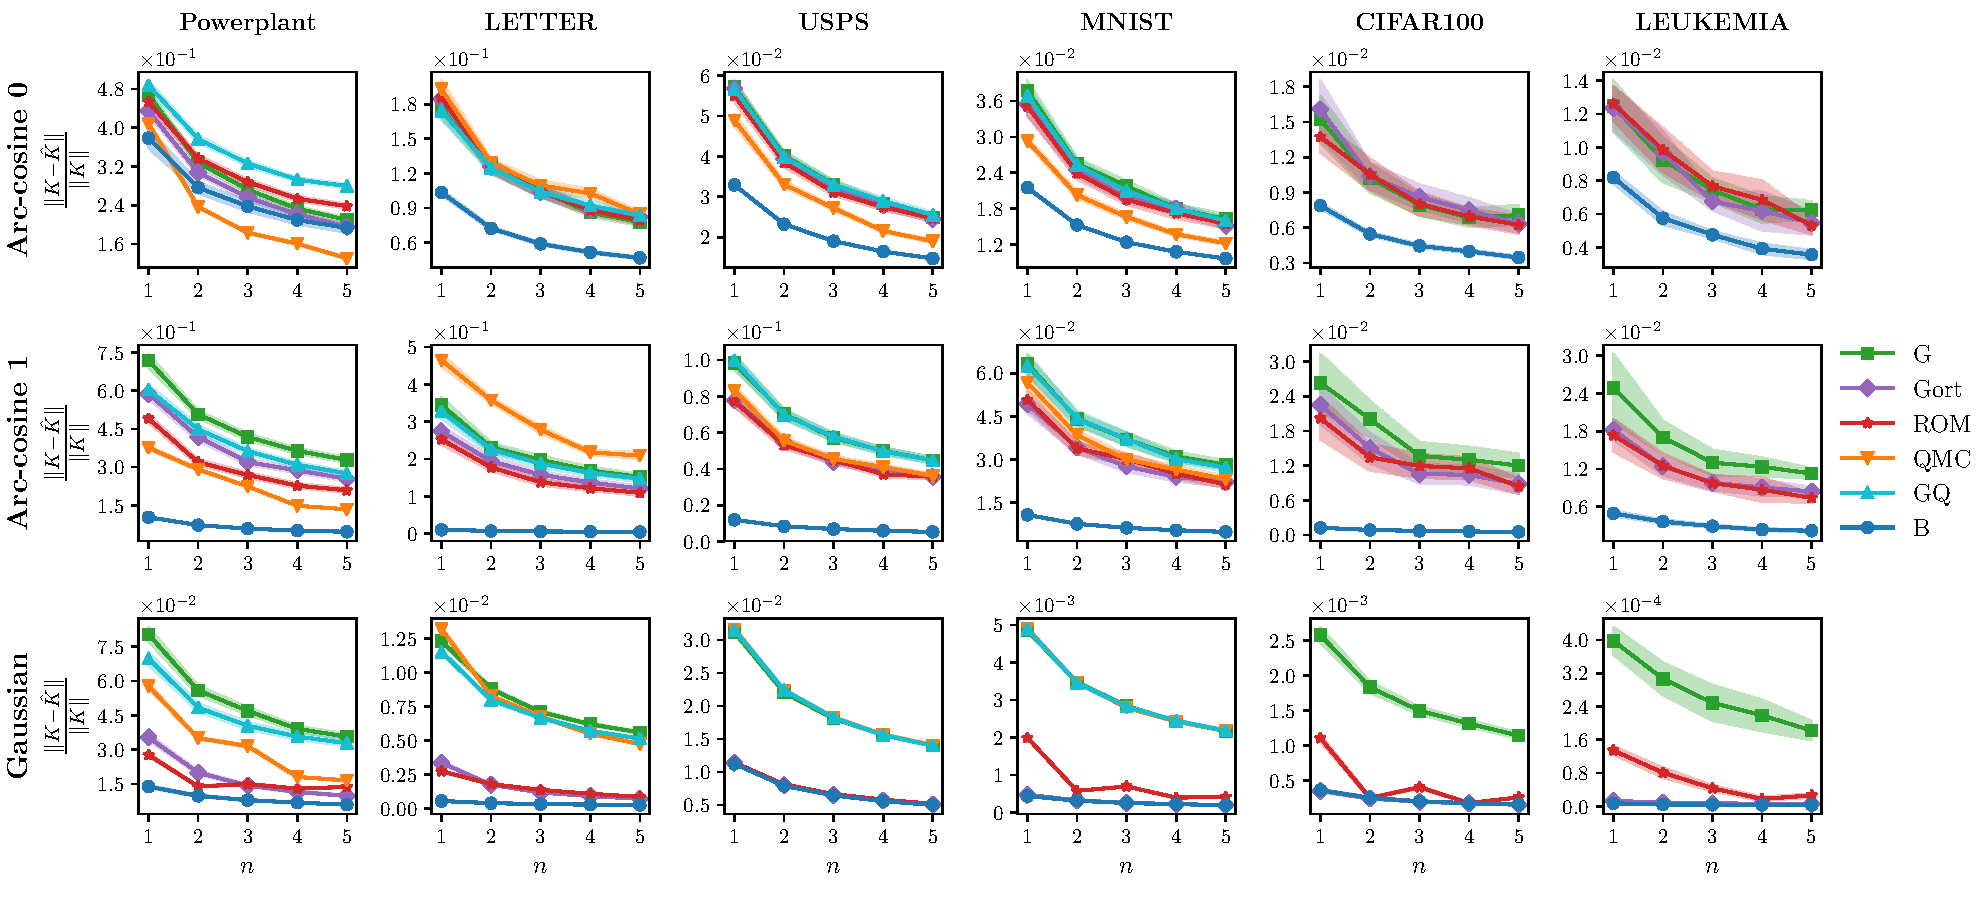
\includegraphics[width=\textwidth]{figures/quadratures/kernel_acc}
\caption{Kernel approximation error across three kernels and 6 datasets.Lower is better. The x-axis represents the factor to which we extend the original feature space, $n = \frac{D}{2(d+1)+1}$, where $d$ is the dimensionality of the original feature space, $D$ is the dimensionality of the new feature space.}
\label{fig:KA}
\end{figure*}
To measure kernel approximation quality we use relative error in Frobenius norm
$\frac{\Vert \mathbf{K} - \mathbf{\hat{K}}\Vert_{F}}{\Vert \mathbf{K} \Vert_{F}}$,
where $\mathbf{K}$ and $\mathbf{\hat{K}}$ denote exact kernel matrix and its approximation.
In line with other works we run experiments for the kernel approximation on a random
subset of a dataset.
Table \ref{table:experimental_setting} displays the settings for the experiments across the
datasets.
\begin{table}[h]
    \centering
    \caption{Space and time complexity.}
    \label{table:complexity}
    \begin{tabular}{ c  c  c }
    \textbf{Method} & \textbf{Space} & \textbf{Time} \\
    \hline
    ORF & $\mathcal{O}(Dd)$ & $\mathcal{O}(Dd)$ \\
    QMC & $\mathcal{O}(Dd)$ & $\mathcal{O}(Dd)$ \\
    ROM & $\mathcal{O}(d)$ & $\mathcal{O}(d\log d)$ \\
    \textbf{Quadrature based} & $\mathcal{O}(d)$ & $\mathcal{O}(d\log d)$ \\
    \hline
    \end{tabular}
\end{table}
\begin{table}[h]
    \centering
    \caption{Experimental settings for the datasets.}
    \label{table:experimental_setting}
    \begin{tabular}{ c c c c c }
    \textbf{Dataset} & $N$ & $d$ & \textbf{\#samples} & \textbf{\#runs} \\
    \hline
    Powerplant & 9568 & 4 & 550 & 500 \\
    LETTER & 20000 & 16 & 550 & 500 \\
    USPS & 9298 & 256 & 550 & 500 \\
    MNIST & 70000 & 784 & 550 & 100 \\
    CIFAR100 & 60000 & 3072 & 50 & 50 \\
    LEUKEMIA & 72 & 7129 & 10 & 10 \\
    \hline
    \end{tabular}
\end{table}

Approximation was constructed for different number of $SR$ samples $n = \frac{D}{2(d+1)+1}$,
where $d$ is an original feature space dimensionality and $D$ is the new one. For the Gaussian
kernel we set hyperparameter $\gamma = \frac{1}{2\sigma^2}$ to the default value of
$\frac{1}{d}$ for all the approximants, while the arc-cosine kernels (see definition of
arc-cosine kernel in the Appendix) have no hyperparameters.

We run experiments for each [kernel, dataset, $n$] tuple and plot 95\% confidence interval around the mean value line. Figure \ref{fig:KA} shows the results for kernel approximation error on LETTER, MNIST, CIFAR100 and LEUKEMIA datasets.

QMC method almost always coincides with RFF except for arc-cosine 0 kernel. It particularly enjoys Powerplant dataset with $d=4$, i.e. small number of features. Possible explanation for such behaviour can be due to the connection with QMC quadratures. The worst case error for QMC quadratures scales with $n^{-1}(\log n)^d$, where $d$ is the dimensionality and $n$ is the number of sample points \citep{owen1998latin}. It is worth mentioning that for large $d$ it is also a problem to construct a proper QMC point set. Thus, in higher dimensions QMC may bring little practical advantage over MC. While recent randomized QMC techniques indeed in some cases have no dependence on $d$, our approach is still computationally more efficient thanks to the structured matrices. GQ method as well matches the performance of RFF. We omit both QMC and GQ from experiments on datasets with large $d = [3072, 7129]$ (CIFAR100, LEUKEMIA).

The empirical results in Figure \ref{fig:KA} support our hypothesis about the advantages of $\mathbf{SR}$ quadratures applied to kernel approximation compared to SOTA methods.
With an exception of a couple of cases: (Arc-cosine 0, Powerplant) and (Gaussian, USPS), our method displays clear exceeding performance.

\subsection{Classification/regression with new features}
\label{sub:finalscore}
\begin{figure*}[h]
\centering
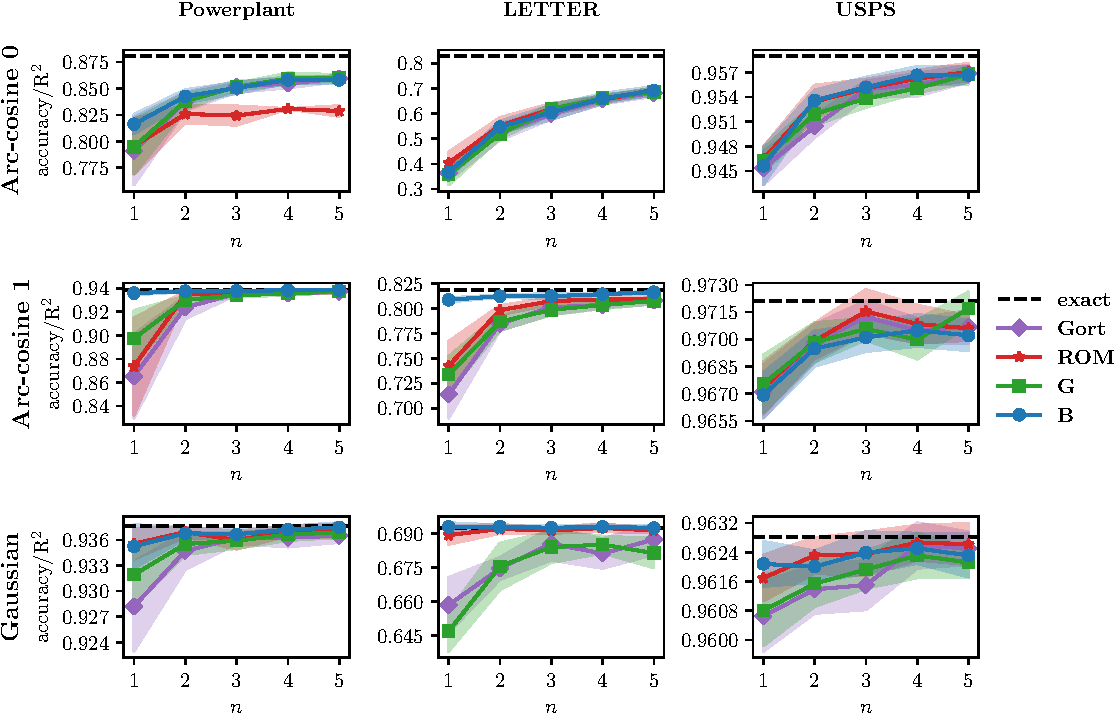
\includegraphics[width=0.8\textwidth]{figures/quadratures/Powerplant_LETTER_USPSacc_plain}
\caption{Accuracy/$R^2$ score using embeddings with three kernels on 3 datasets. Higher is better.
The x-axis represents the factor to which we extend the original feature space, $n = \frac{D}{2(d+1)+1}$.}
\label{fig:acc}
\end{figure*}

We estimate accuracy and $R^2$ scores for the classification/regression tasks on some of the datasets (Figure~\ref{fig:acc}).
We examine the performance with the same setting as in experiments for kernel approximation error, except now we map the whole dataset.
We use Support Vector Machines to obtain predictions.

Kernel approximation error does not fully define the final prediction accuracy -- the best performing kernel matrix approximant not necessarily yields the best accuracy or $R^2$ score. However, the empirical results illustrate that our method delivers comparable and often superior quality on the downstream tasks.

\subsection{Walltime experiment}
We measure time spent on explicit mapping of features by running each experiment 50 times and averaging the measurements.  Indeed, Figure \ref{fig:walltime} demonstrates that the method scales as theoretically predicted with larger dimensions thanks to the structured nature of the mapping.

\begin{figure}[h]
\centering
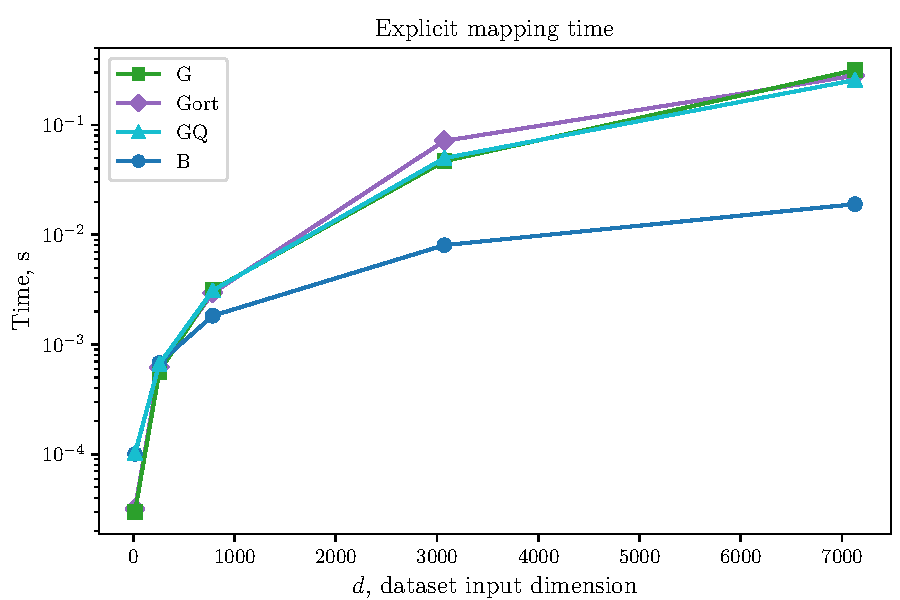
\includegraphics[width=0.4\textwidth]{figures/quadratures/time_r}
\caption{Time spent on explicit mapping. The x-axis represents the 5 datasets with increasing input number of features: LETTER, USPS, MNIST, CIFAR100 and LEUKEMIA.}
\label{fig:walltime}
\end{figure}

\section{Related work}
\label{sec:related_work}
In this section we provide brief review of the existing approaches
connected to the low-rank approximation of the kernel function.

The most popular methods for scaling up kernel methods are based on a low-rank approximation of the kernel using either data-dependent or independent basis functions.
The first one includes Nystr{\" o}m method \citep{drineas2005nystrom}, greedy basis selection techniques \citep{smola2000sparse}, incomplete Cholesky decomposition \citep{fine2001efficient}.

The construction of basis functions in these techniques utilizes the given training set making them more attractive for some problems compared to Random Fourier Features approach.
In general, data-dependent approaches perform better than data-independent approaches when there is a gap in the eigen-spectrum of the kernel matrix.
The rigorous study of generalization performance of both approaches can be found in \citep{yang2012nystrom}.

In data-independent techniques, the kernel function is approximated directly.
Most of the methods (including the proposed approach) that follow this idea are based on Random Fourier Features \citep{rahimi2008random}. They require so-called weight matrix that can be generated in a number of ways.
\citep{le2013fastfood} form the weight matrix as a product of
structured matrices.
It enables fast computation of matrix-vector products and speeds up generation of random features.

Another work \citep{felix2016orthogonal} orthogonalizes the features by means of orthogonal weight matrix.
This leads to less correlated and more informative features increasing the quality of approximation. They support this result both analytically and empirically.
The authors also introduce matrices with some special structure for fast computations.
\citep{choromanski2017unreasonable} propose a generalization of the ideas from \citep{le2013fastfood} and \citep{felix2016orthogonal}, delivering an analytical estimate for the mean squared error (MSE) of approximation.

All these works use simple Monte Carlo sampling.
However, the convergence can be improved by changing Monte Carlo sampling to Quasi-Monte Carlo sampling.
Following this idea \citep{yang2014quasi} apply quasi-Monte Carlo to Random Fourier Features.
In \citep{yu2015compact} the authors make attempt to improve quality of the approximation of Random Fourier Features by optimizing sequences conditioning on a given dataset.

Among the recent papers there are works that, similar to our approach, use the numerical integration methods to approximate kernels. While \citep{bach2017equivalence} carefully inspects the connection between random features and quadratures, they did not provide any practically useful explicit mappings for kernels. Leveraging the connection \citep{dao2017gaussian} propose several methods with Gaussian quadratures. Among them three schemes are data-independent and one is data-dependent. The authors do not compare them with the approaches for random feature generation other than random Fourier features. The data-dependent scheme optimizes the weights for the quadrature points to yield better performance.

\chapter{Applications}
\label{chap:applications}

This chapter is dedicated to the applications of the developed techniques
in several different problems.
We demonstrate how the described approaches for GP regression
and kernel approximation can be used in a tensor completion
problem,
density estimate, and simultaneous localization and mapping (SLAM).
This is a diverse set of problems: density estimation is a key problem
in statistics, SLAM is one of the main problems in robotics,
while tensor completion is a very general problem, which can be encountered
in computer vision, signal processing, machine learning and many others.
All of them require large-scale or online methods and can benefit
from using GP- or kernel-based approaches.
In this chapter, we show how large-scale GP methods can be incorporated into
existing approaches.
The resulting techniques provide state-of-the-art results in terms of both
accuracy and computational complexity.

Section \ref{sec:tensor_completion_using_gp} describes our approach for
tensor completion using Gaussian Processes.
Our contributions here are the following:
\begin{itemize}
    \item We consider the case when the tensor is generated by some smooth function.
    Using this assumption, we propose an initialization approach that
    can be used with a wide range of tensor completion techniques.
    \item We demonstrate empirically on real-world problems that different optimization methods
    for tensor completion benefit from using the proposed initialization.
    It considers assumption about tensor generating function and, therefore, allows to increase generalization power.
\end{itemize}
In section \ref{sec:score_matching} we develop randomized feature maps-based approach for density estimation.
We seek our solution in kernel exponential family of distributions with the denoising score matching loss function.
Our main results are as follows:
\begin{itemize}
    \item We derived an analytical solution for the described setup.
    \item We show that our solution has implicit regularization in contrast
    to other approaches that usually add special regularization term based on higher
    order derivatives of the probability density function.
    \item Finally, we demonstrate the benefits of the proposed approach on a set of different
    benchmarks and compare it with other techniques.
\end{itemize}
The last section \ref{sec:SLAM} is devoted to GP models with random feature approximations
in SLAM problem.
The GP model is used here to model state of the robot depending on time.
We contribute to this field by
\begin{itemize}
    \item Developing an approach based on random features for time-continuous SLAM.
    \item Compared to other state-of-the-art approaches, our method is more accurate
    in case of noisy observations because we do not assume the sparse structure of the
    inverse covariance matrix. We demonstrate it on a set of synthetic benchmarks
    as well as real-world problems.
\end{itemize}

\section{Tensor Completion using Gaussian Processes}
\label{sec:tensor_completion_using_gp}

In this section, we consider the tensor completion problem.
We suppose that values of tensor $\mathcal{X}$ are generated by some smooth function, i.e.
\[
\mathcal{X}_{i_1, \ldots, i_d} = f(x_{i_1}, \ldots, x_{i_d}),
\]
where $(x_{i_1}, \ldots, x_{i_d})$ is a point on
some multi-dimensional grid and $f(\cdot)$ is some
unknown smooth function.
However, the tensor values are known only at some small subset of the grid.
The task is to complete the tensor, i.e., to reconstruct the tensor values at all points on the grid considering the properties of the {\em data generating process} $f(\cdot)$.

This problem statement differs from the traditional problem statement, which does not use any assumptions about the function $f(\cdot)$.
Knowing some properties of the data generating function provides insights about how the tensor values relate to each other, and this, in turn, allows us to improve the results.
In this work, we assume that function $f(\cdot)$ is smooth.

% Such a problem statement is rarely taken into account in literature.
There are a lot of practical applications that suit the statement.
For example, modeling of physical processes, solutions of differential equations, modeling probability distributions.

Here, we propose to model the smoothness of the data generating process using
GP Regression (GPR).
In GPR, the assumptions about the function that we approximate are controlled via the kernel
function.
The GPR model is then used to construct the initial solution to the tensor completion problem.
% by applying Tensor-Train cross-approximation technique (TT-cross).

In principle, such initialization can improve any other tensor completion technique.
It means that using the proposed initialization state-of-the-art results
can be obtained by employing some simple optimization procedure like the Stochastic Gradient Descent.


When the tensor order is high, the problem should be solved in some low-rank
format because the number of elements of the tensor grows exponentially.
The proposed approach is based on the tensor train (TT) format for its
computational efficiency and ability to handle large dimensions \citep{oseledets2010tt}.

% The contributions of this paper are as follows
% \begin{itemize}
% \item[--] We introduce new initialization algorithm which considers the tensor generating process.
% The proposed algorithm is described in \cref{sec:tensor_completion_init}.
% \item[--] The proposed initialization technique automatically selects the rank of the tensor. The details are given in \cref{sec:tt_cross}.
% \item[--] We conducted empirical evaluations of the proposed approach and compared it with tensor completion techniques without our initialization.
% The results are given in \cref{sec:tensor_completion_experiments} and show the superiority of the proposed algorithm.
% \end{itemize}


\subsection{Tensor completion}
\label{sec:tensor_completion}

The formal problem statement is as follows.
Suppose $\mathcal{Y}$ is a $d$-way tensor,
$\mathcal{Y} \in \mathbb{R}^{n_1 \times n_2 \times \cdots \times n_d}$
(by tensor here we mean a multi-dimensional array).
Tensor values are known only at some subset of indices
$\Omega \subset \{1, \ldots, n_1\} \times \cdots \times \{1, \ldots, n_d\}$.
By $P_\Omega$ we denote the projection onto the set $\Omega$, i.e.
\[
P_{\Omega} \mathcal{X} = \mathcal{Z}, \quad
\mathcal{Z}(i_1, i_2, \ldots, i_d) = \begin{cases}
\mathcal{X}(i_1, i_2, \ldots, i_d) & \mbox{if } (i_1, \ldots, i_d) \in \Omega, \\
0 & \mbox{otherwise}.
\end{cases}
\]
We formulate the tensor completion as an optimization problem
\begin{equation}
\begin{aligned}
\label{eq:tensor_completion}
    \min_{\mathcal{X}} \quad &  f(\mathcal{X}) = \|P_{\Omega} \mathcal{X} - P_{\Omega} \mathcal{Y}\|_F^2 \\
    \mbox{subject to} \quad & \mathcal{X} \in \mathcal{M}_r =
    \{\mathcal{X} \in \mathbb{R}^{n_1 \times \cdots n_d} \; | \; {\rm rank}_{TT}
    (\mathcal{X}) = \mathbf{r} \},
\end{aligned}
\end{equation}
where ${\rm rank}_{TT}(\mathcal{X})$ is a tensor train rank of $\mathcal{X}$ \citep{oseledets2011tensor},
which is a generalization of the matrix rank,
and $\|\cdot\|_F$ is the Frobenius norm.
A tensor $\mathcal{X}$ is said to be in tensor train format if its elements are represented as
\[
    \mathcal{X}(i_1, \ldots, i_d) = \sum_{j_1, j_2, \ldots j_d}
    \mathcal{G}^{(1)}_{1, i_1, j_1}
    \mathcal{G}^{(2)}_{j_1, i_2, j_2} \cdots
    \mathcal{G}^{(d)}_{j_{d - 1}, i_d, 1},
\]
where $\mathcal{G}^{(i)}$ is a three-way tensor core with size
$r_{i - 1} \times n_i \times r_{i}$, $r_0 = r_{d} = 1$.
Vector $\mathbf{r}_{TT} = (r_0, \ldots, r_d)$ is called TT-rank.

Tensor train format assumes that the full tensor can be approximated by
a set of $3$-way core tensors, the total number of elements in
core tensors is $\mathcal{O}(dnr^2)$, where
$r = \max\limits_{i = 0, \ldots, d}\{r_i\}$,
$n = \max\limits_{i = 1, \ldots, d}\{n_i\}$,
which is much smaller than $n^d$.

In problem \eqref{eq:tensor_completion}, we optimize the objective
function straightforwardly with respect to tensor cores
$\mathcal{G}^{(1)}, \ldots \mathcal{G}^{(d)}$ while having their sizes fixed.
Problem \eqref{eq:tensor_completion} is non-convex, so
optimization methods can converge to a local minimum.
To get an efficient solution, we impose two requirements:
\begin{enumerate}
    \item Initial tensor $\mathcal{X}_0$ in tensor train format should be as close to the optimum as possible.
    \item Availability of an efficient optimization procedure that will be launched from the obtained initial tensor.
\end{enumerate}
These steps are independent, and one can apply any desired algorithm in each of them.

In this section, we develop the initialization algorithm, which allows obtaining accurate initial tensor for the case when the tensor of interest is generated by some smooth function.
The experimental section below demonstrates that our initialization can improve the results of
many optimization procedures and shows the potential of our approach to be adapted
to a large number of different tensor completion techniques.


\subsection{Initialization}
\label{sec:tensor_completion_init}
We consider tensors that are generated by some function,
i.e., tensor values are computed as follows
\[
\mathcal{Y}_{i_1, \ldots, i_d} = f(x_{i_1}, \ldots, x_{i_d}),
\]
where $f(\cdot)$ is some unknown smooth function and
$(x_{i_1}, \ldots, x_{i_d})^\top \in \mathbb{R}^d$,
$i_k = 1, \ldots, n_k$,
$n_1, \ldots, n_d$ are tensor sizes.
The set of points $\{(x_{i_1}, \ldots x_{i_d}): i_k = 1, \ldots, n_k; k = 1, \ldots, d\}$ is a full factorial DoE, i.e., a multi-dimensional grid,
and we also assume that the grid is uniform.

In this setting, the tensor completion can be considered a regression problem and can be solved by any regression technique that guarantees the smoothness of the solution.
However, in the tensor completion problem, we are interested in a tensor of values of $f(\cdot)$ at a predefined finite grid of points.
The tensor should be in a low-rank format to be able to perform various operations with the tensor efficiently (e.g., calculation of the norm of the tensor, dot product and other).

These observations give us the solution: build regression model $\widehat{f}$ using the observed values of the tensor, then use the obtained approximation as a black-box for the TT-cross approximation algorithm \citep{oseledets2010tt}.
The last step results in a tensor $\widehat{\mathcal{X}}$ in TT format, which is a low-rank format and allows efficient computations.
The next step (which is optional) is to improve the obtained solution $\widehat{\mathcal{X}}$ by using it as initialization for any other tensor completion technique.

% As a result, we will obtain an approximate model $\widehat{f}$ that can
% compute the tensor value at any index.
% When we have tensor generating function $\widehat{f}$ the tensor completion problem
% can be efficiently solved using Tensor-Train cross-approximation (TT-cross)
% \citep{oseledets2010tt}.
% However, as $\widehat{f}$ is just approximation of the actual function $f$
% the results of TT-cross can be further improved using the given
% actual values of the tensor $\mathcal{X}$.

Let us write down the set of observed tensor values into a vector $\mathbf{y}$
and the corresponding indices into a matrix $\mathbf{X}$ (each row is a vector of indices
$(i_1, i_2, \ldots, i_d)$).
Then, the approach for tensor completion (in TT format) can be
written as follows

\begin{enumerate}
    \item Construct initial tensor $\mathcal{X}_0$ in TT format:
        \begin{enumerate}
        \item Apply some regression technique using the given data set $(\mathbf{X}, \mathbf{y})$ to construct approximation of the function that generates tensor values.
        \item Apply TT-cross method (see Section~\ref{sec:tt_cross}, \citep{oseledets2010tt}) to the constructed approximation to obtain $\mathcal{X}_0$.
        \end{enumerate}
    \item Apply some tensor completion technique using $\mathcal{X}_0$
    as an initial value.
\end{enumerate}

At step $1$(a), the choice of the regression technique affects
the result of the initialization, although it can be arbitrary.
It is required to choose the regression algorithm such that it will capture the peculiarities of the tensor we would like to restore.
As we stated above, we suppose that the tensor generating function is smooth
(which is a common situation when modeling physical processes).
Therefore, we choose a regression technique that is good at approximating smooth functions.
A reasonable choice, in this case, is to use Gaussian Process Regression.
GP models is a favorite tool in many engineering applications as they have
proved to be efficient, especially for problems where it is required to
model some smooth function \citep{belyaev2016gtapprox}.
The points $(x_{i_1}, \ldots, x_{i_d})$ are not given; all we know is that at the point with multi-index
$(i_1, \ldots, i_d)$ on the grid the function value
is equal to $\mathcal{X}_{i_1, \ldots, i_d}$.
To make the problem statement reasonable we assume that
the indices are connected with the points as follows:
$x_{i_k} = a_k i_k + b_k$,
where $a_k, b_k \in \mathbb{R}$.
So, as an input for the approximation, we set $a_k$ and $b_k$ such that $x_{i_k} \in [0, 1]$.

At step $1$(b), we use TT-cross
because it allows to efficiently approximate black-box function by a low-rank tensor in TT format.
Moreover, this approach can automatically select TT-rank, making it more desirable.
More details on the technique are given in Section~\ref{sec:tt_cross}.

The described approach has the following benefits:
\begin{enumerate}
    \item Initial tensor $\mathcal{X}_0$, which is close to the optimal value in terms of the reconstruction error at observed values.
    It will push the optimization to faster convergence.
    \item Better generalization ability: there are many degrees of freedom. A lot of different tensor train factors can give low reconstruction error at observed positions but can give a large error at other locations.
    Accurate approximation model will push the initial tensor to be closer to the original tensor in both the observed positions and unobserved ones.
    \item TT-cross technique chooses rank automatically, so there is no need to tune the rank of the tensor manually.
\end{enumerate}

The described approach leads to the Algorithm~\ref{alg:initialization}.
Steps 3 and 4 of the algorithm are described in
Sections~\ref{sec:intro} and \ref{sec:tt_cross}, respectively.

\begin{algorithm}
\caption{Initialization}
\label{alg:initialization}
    \hspace*{\algorithmicindent} \textbf{Input}: $\mathbf{y}, \Omega$ \\
    \hspace*{\algorithmicindent} \textbf{Output}: $\mathcal{Y}_0$ in tensor train format
    \begin{algorithmic}[1]
        \State Construct the training set $(\mathbf{X}, \mathbf{y})$ from $\mathbf{y}, \Omega$
        \State Rescale inputs $\mathbf{X}$ to $[0, 1]$ interval
        \State Using $(\mathbf{X}, \mathbf{y})$ build GP model $\hat{f}(\mathbf{x})$
        \algorithmiccomment{see Section~\ref{sec:intro} for details}
        \State Apply TT-cross to $\hat{f}(\mathbf{x})$ and obtain $\mathcal{Y}_0$
        \algorithmiccomment{see Section~\ref{sec:tt_cross} for details}

        \State \Return $\mathcal{Y}_0$
    \end{algorithmic}
\end{algorithm}

% \subsection{Gaussian Process Regression}
% \label{sec:gp}
% One of the most efficient tools for approximating smooth functions is the Gaussian Process (GP)
% Regression \citep{burnaev2016regression}.
% GP regression is a Bayesian approach where a prior distribution over continuous functions
% is assumed to be a Gaussian Process, i.e.,
% \[
%   \mathbf{y} \, | \, \mathbf{X} \sim \mathcal{N}(\boldsymbol{\mu}, \, \mathbf{K}_f + \sigma_{noise}^2\mathbf{I}),
% \]
% where $\mathbf{y} = (y_1, y_2, \ldots, y_N)$ is a vector of outputs,
% $\mathbf{X} = (\mathbf{x}_1^{\top}, \mathbf{x}_2^{\top}, \ldots, \mathbf{x}_N^{\top})^{\top}$ is a matrix of inputs,
% $\mathbf{x}_i \in \mathbb{R}^d$,
% $\sigma_{noise}^2$ is a noise variance,
% $\boldsymbol{\mu} = (\mu(\mathbf{x}_1), \mu(\mathbf{x}_2), \ldots, \mu(\mathbf{x}_N))$ is a mean vector modeled by some function $\mu(\mathbf{x})$,
% $\mathbf{K}_f = \{ k(\mathbf{x}_i, \mathbf{x}_j) \}_{i, j = 1}^N$ is a covariance matrix for some a priori selected covariance function $k$ and
% $\mathbf{I}$ is an identity matrix.
% An example of such function is a squared exponential kernel
% \[
% k(\mathbf{x}, \mathbf{x}') = \exp \left (
% - \frac{1}{2} \sum_{i=1}^d \left (
% \frac{\mathbf{x}^{(i)} - \mathbf{x}'{}^{(i)}}{\sigma_i}
% \right )^2
% \right ),
% \]
% where $\sigma_i, i = 1, \ldots, d$ are parameters of the kernel
% (hyperparameters of the GP model).
% The hyperparameters should be chosen according to the given data set.

% Without loss of generality, we make the standard assumption of zero-mean data.
% Now, for a new unseen data point $\mathbf{x}_*$ we have
% \begin{equation}
% \label{eq:gp_posterior}
%     \hat{f}(\mathbf{x}_*) \sim \mathcal{N}\left (\mu(\mathbf{x}_*), \sigma^2(\mathbf{x}_*) \right ),
% \end{equation}
% \[
%     \mu(\mathbf{x}_*) = \mathbf{k}(\mathbf{x}_*)^\top \mathbf{K}_y^{-1}\mathbf{y},
% \]
% \[
%     \sigma^2(\mathbf{x}_*) = k(\mathbf{x}_*, \mathbf{x}_*) - \mathbf{k}(\mathbf{x}_*)^\top \mathbf{K}_y^{-1} \mathbf{k}(\mathbf{x}_*),
% \]
% where $\mathbf{k}(\mathbf{x}_*) = (k(\mathbf{x}_*, \mathbf{x}_1), \ldots, k(\mathbf{x}_*, \mathbf{x}_N))^T$ and
% $\mathbf{K}_y = \mathbf{K}_f + \sigma_{noise}^2\mathbf{I}$.

% % Usually for GP regression, a squared exponential covariance function is used
% % \begin{equation}
% %   \label{eq:covariance_function}
% %   k(\mathbf{x}_p, \mathbf{x}_q) = \sigma_f^2 \exp \left ( -\sum_{i = 1}^d \theta_i^2 (\mathbf{x}_p^{(i)} - \mathbf{x}_q^{(i)})^2 \right ).
% % \end{equation}

% Let us denote the vector of hyperparameters $\sigma_i, i=1, \ldots, d, \sigma_f$ and $\sigma_{noise}$ by $\boldsymbol{\theta}$. % = (\theta_1, \ldots, \theta_d)$.
% To choose the hyperparameters of our model, we consider the log-likelihood
% \[
%     \log p(\mathbf{y} \, | \, \mathbf{X}, \boldsymbol{\theta}) =
%     -\frac12 \mathbf{y}^T \mathbf{K}_y^{-1}\mathbf{y} - \frac12 \log |\mathbf{K}_y| -
%     \frac{N}{2} \log 2 \pi
% \]
% and maximize it over the hyperparameters \citep{rasmussen2004gaussian}.
% The runtime complexity of learning GP regression is $\mathcal{O}(N^3)$ as we need to calculate the inverse of $\mathbf{K}_y$, its determinant and derivatives of the log-likelihood.
% If the sample size $N$ ($|\Omega|$ in our case) is large, the computational complexity becomes an
% issue.
% There are several ways to overcome it.
% If the data set has a factorial structure (multidimensional grid in a simple
% case), we can use the algorithm from \citep{belyaev2015gaussian}.
% If the structure is factorial with a small number of missing values
% the method from \citep{belyaev2016computationally} should be applied.
% For general unstructured cases, the approximate GP model can be built
% using, for example, the model described in \citep{munkhoeva2018quadrature} or use a subsample as a training set.

% After tuning of the hyperparameters, we can use the mean of the posterior distribution
% \eqref{eq:gp_posterior} as a prediction of the model.

% Note that the input points $\mathbf{X}$ in our case is a set of indices of the
% observed values $\mathbf{y}$.
% For the GP model, we scale each index to $[0, 1]$ interval.
\subsubsection{Kernel choice and smoothness assumption}
We approximate function $f$ using the GP model.
The GP model is a function from some reproducing kernel Hilbert space (RKHS) $\mathcal{H}$ which is fully defined by the kernel function.
Ideally, the function $f$ should be from the Hilbert space $\mathcal{H}$.
However, for a given kernel function, it can be difficult to identify what functions lie in the corresponding RKHS.

In practice, GP models with popular kernels (RBF kernel, Mat{\'{e}}rn kernel) provide good results, when $f \in C^k$, $k \ge 1$.
So, in the experiments section, we assume that the functions are from this class of functions and use RBF kernel.

\subsubsection{Tensor-Train cross-approximation}
\label{sec:tt_cross}
To approximate tensor $\widehat{\mathcal{X}}$ generated by $\hat{f}$, we use Tensor-Train cross-approximation.
First, let us consider the matrix case.
Suppose we are given a rank-$r$ matrix $\mathbf{A}$ of size $m \times n$.
A cross-approxi\-mation for the matrix is represented as
\[
    \mathbf{A} = \mathbf{C} \widehat{\mathbf{A}}^{-1} \mathbf{R},
\]
where $\mathbf{C} = \mathbf{A}(:, J), \mathbf{R} = \mathbf{A}(I, :)$ are some $r$ columns and rows of the matrix $\mathbf{A}$ and $\widehat{\mathbf{A}} = A(I, J)$ is the submatrix on the intersection of these rows and columns. To construct accurate approximation, it is required to find submatrix $\widehat{\mathbf{A}}$ of large volume.
It can be done in $\mathcal{O}(nr^2)$ operations \citep{tyrtyshnikov2000incomplete}.

Now for tensor $\widehat{\mathcal{X}} \in \mathbb{R}^{n_1 \times \cdots \times n_d}$ the procedure is the following.
At the first step, let us consider unfolding $\mathbf{X}_1$ of size
$n_1 \times n_2 n_3 \cdot \cdots \cdot n_d$ and rank $r_1$.
Using row-column alternating algorithm from \citep{tyrtyshnikov2000incomplete}, we can find $r_1$ linearly independent columns of matrix $\mathbf{X}_1$, these columns form matrix $\mathbf{C}$.
After that, by applying maxvol procedure \citep{tyrtyshnikov2000incomplete} to the matrix $\mathbf{C}$, we can find a set of row indices $I_1 = \big[i_1^{\alpha_1} \big], \alpha_1 = 1, \ldots, r_1$, matrix $\mathbf{R}$ and matrix $\widehat{\mathbf{A}}_1$
that will give the cross-approximation of unfolding $\mathbf{X}_1$:
\[
    \mathbf{X}_1 = \mathbf{C}\widehat{\mathbf{A}}_1^{-1}\mathbf{R}.
\]
We set
\[
    \mathbf{G}_1 = \mathbf{C}\widehat{\mathbf{A}}_1^{-1},
\]
where $\mathbf{G}_1$ is of size $n_1 \times r_1$.
Next, let us form tensor $\mathcal{R}$ from $r_1$ rows of $\mathbf{X}_1$:
\[
    \mathcal{R}(\alpha_1, i_2, \ldots, i_d) = \widehat{\mathcal{X}}(i_1^{\alpha_1}, i_2, \ldots, i_d),
\]
and reshape it into a tensor of size $r_1n_2 \times n_3 \times \cdots \times n_d$.
The next step is to apply the same procedure to the unfolding $\mathbf{R}_1$ of the tensor $\mathcal{R}$ and obtain the matrices $\mathbf{C}$, $\widehat{\mathbf{A}}_2$ and
\[
    \mathbf{G}_2 = \mathbf{C} \widehat{\mathbf{A}}_2^{-1}
\]
of size $r_1n_2 \times r_2$.

Repeating the described procedure $d$ times, we will end up with matrices
$\mathbf{G}_1, \allowbreak \mathbf{G}_2, \ldots, \mathbf{G}_d$ of sizes $n_1 \times r_1, r_1n_2 \times r_2, \ldots, r_{d-1}n_d \times 1$.
Then, each matrix can be reshaped to the $3$-way tensor of size $r_{d - 1} \times n_d \times r_d$,
$r_0 = r_d = 1$ and can be used as core tensors for TT format.
It turns out that such representation is a TT decomposition of the initial tensor $\widehat{\mathcal{X}}$.

The exact ranks $r_1, \ldots, r_d$ are not known to us in general.
They can only be estimated from the above (e.g., by the maximum rank of the corresponding unfolding).
If the rank is overestimated, then the calculation of matrices $\mathbf{G}_i$
is an unstable operation (because we obtain almost rank-deficient unfolding matrices).
However, in \citep{oseledets2010tt}, the authors suggest some simple modifications that overcome this issue.
Therefore, we need to estimate the ranks from the above, but
the estimate should not be much larger than the real rank.
So, the approach is to start from some small rank, construct the tensor
in TT format and then apply recompression (see \citep{oseledets2011tensor}).
If there is a rank that is not reduced, then we underestimated that rank and should then increase it and repeat the procedure.

\subsubsection{Computational complexity}
The computational complexity of TT cross-approximation method is as follows.
To perform the procedure, we need to evaluate the GP model $\mathcal{O}(dnr^2)$ times at some subset of grid points
and then perform $\mathcal{O}(dnr^3)$ operations to find all maximum volume submatrices.
The complexity of evaluating the GP model at one point is $\mathcal{O}(Nd)$, where $N$ is the number of observed tensor elements.
The total complexity is thus $\mathcal{O}(Nd^2nr^2 + dnr^3)$.

\subsection{Experimental results}
\label{sec:tensor_completion_experiments}
In this section, we present the results of the application of our approach
to two engineering problems and also test it on some artificial problems to investigate how its properties depend on smoothness.

The experimental setup is the following.
We try the following optimization algorithms
\begin{enumerate}
    \item SGD -- stochastic gradient descent \citep{zhao2018high},
    \item Ropt -- Riemannian optimization \citep{steinlechner2016riemannian},
    \item TTWopt -- weighted tensor train optimization \citep{zhao2018high},
    % \item ADF  -- alternating directions fitting \citep{grasedyck2013alternating},
    \item ALS  -- alternating least squares \citep{grasedyck2013alternating}.
\end{enumerate}
We run each algorithm with random initialization and with the
proposed GP-based initialization and then compare the results.


\subsubsection{Functions generated from GP prior}
In order to study the dependence of the solution on the smoothness of the generating function, we applied the proposed approach to the toy functions generated from GP prior with different kernels.
The smoothness of the generated functions is the same as the kernel that we used to generate them.
Thus, we can investigate the performance of the approach for different smoothness.
We considered shift-invariant kernels, i.e. $k(\mathbf{x}, \mathbf{y}) = k(r)$, where $r = \|\mathbf{x} - \mathbf{y}\|$.
The list of kernels is as follows:
\begin{itemize}
    \item Exponential kernel
    \[
        k(r) = \exp \left ( -\frac{r}{\sigma} \right ).
    \]
    The kernel is not differentiable at $\mathbf{x} = \mathbf{y} = 0$, thus
    the functions generated with this kernel are from $C^0$.
    \item Matern$_{3/2}$
    \[
        k_{3/2}(r) = \left (1 + \frac{\sqrt{3}r}{\sigma} \right )
        \exp \left ( -\frac{\sqrt{3}r}{\sigma} \right).
    \]
    This kernel is $1$-time differentiable.
    \item Matern$_{5/2}$
    \[
        k_{5/2}(r) = \left (1 + \frac{\sqrt{5}r}{\sigma} + \frac{5r^2}{3\sigma^2}\right )
        \exp \left ( -\frac{\sqrt{5}r}{\sigma} \right).
    \]
    This kernel is $2$-times differentiable.
    \item Radial Basis Function (RBF) kernel
    \[
        k(r) = \exp \left ( -\frac{r^2}{2\sigma^2} \right ).
    \]
    This kernel is infinitely differentiable.

\end{itemize}
Note that despite the fact that the functions were generated using different kernel functions
in the proposed approach, we used RBF kernel.

To compare how much one approach is better than the other, we calculate the relative MSE error
\[
    {\rm MSE_{rel}} = \frac{1}{\lvert \Omega_{test}\rvert} \left \|\frac{P_{\Omega_{test}}\hat{\mathcal{Y}} -
      P_{\Omega_{test}}\mathcal{Y}}
      {\hat{\sigma}}\right \|_F^2,
\]
where $\Omega_{test}$ is some set of indices independent from the given observed set of indices $\Omega$, $|\Omega_{test}|$ is a size of the set $\Omega_{test}$ and $\widehat{\mathcal{Y}}$ is an obtained approximation of the actual tensor $\mathcal{Y}$,
$\hat{\sigma}$ is a standard deviation of $P_{\Omega_{test}}\mathcal{Y}$.
Such error can be interpreted as the ratio of unexplained variance.
For each optimization technique, we calculate the difference between the error obtained using random initialization and the error obtained using GP based initialization.

For each kernel function, we generated several data sets with different number of observed points ($N \in \{100, 500, 1000, 2000, 5000\}$) and different dimensionalities ($d \in \{2, 3, \ldots, 10, 11, 13, \ldots, 19\} $).
The quantity is illustrated in Figure \ref{fig:improvement} (note that we clamp the values to $[-1, 1]$ interval to make the figures more illustrative).
It shows the improvement of one initialization over another.
We can see from the figure that in most cases, GP-based initialization gives high improvement in the relative error.
The only exception is TTWopt method for which the benefit of the proposed initialization scheme takes place only in about half of the cases.
You can also note white squares for TTWopt; they mean that the implementation of TTWopt crashed for the given data set (for some unknown reason).


\begin{figure}
    \centering
    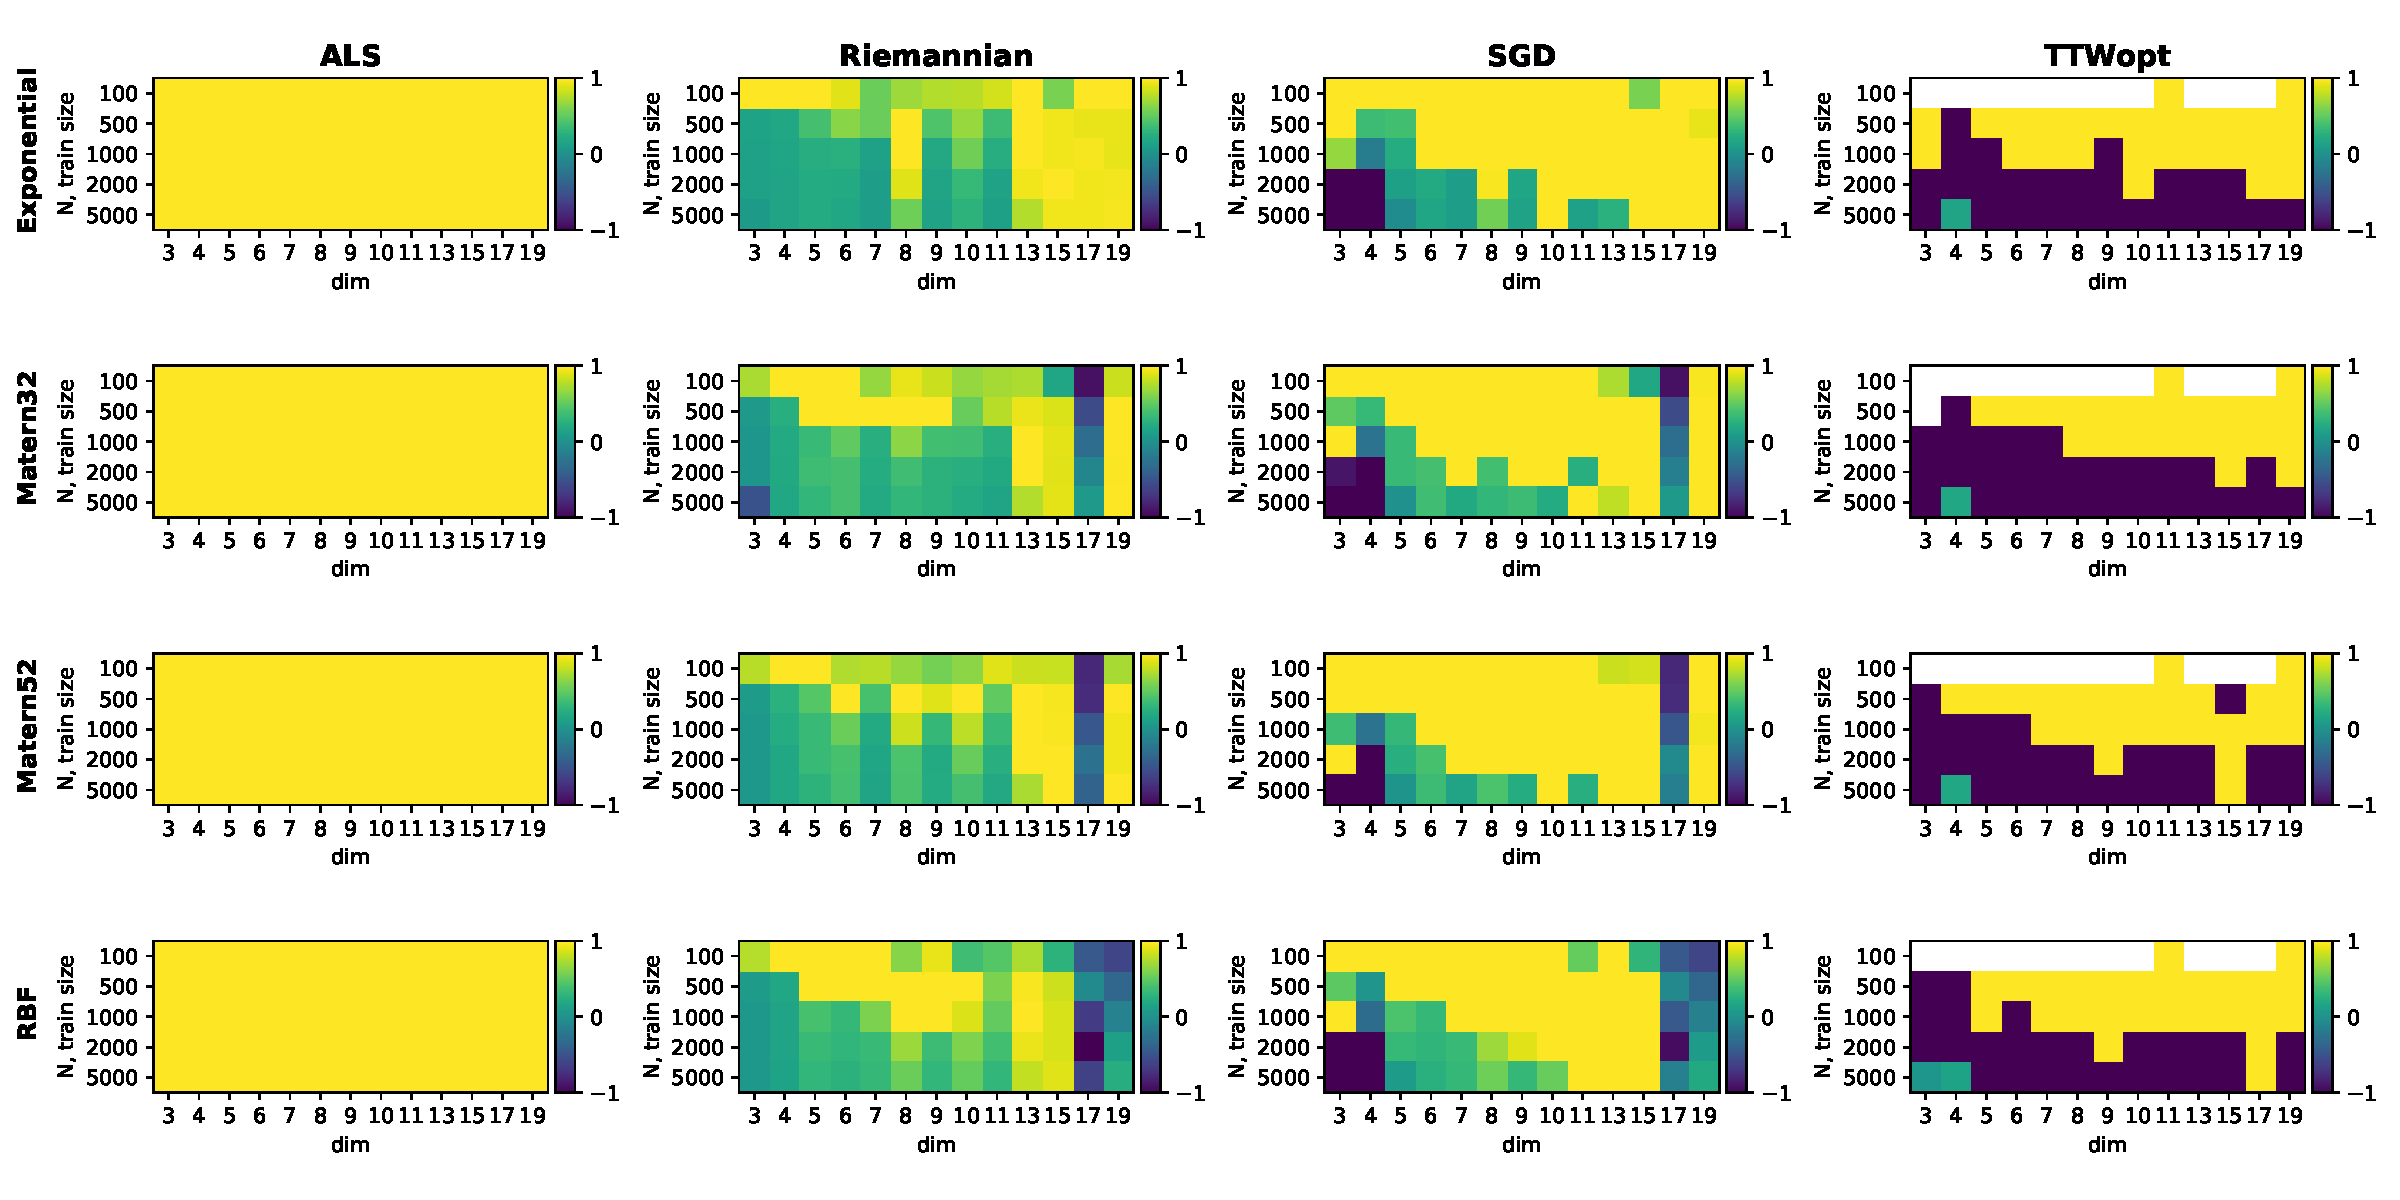
\includegraphics[width=\textwidth]{figures/tensor_completion/gain.pdf}
    \caption{Improvement of GP based initialization over random initialization for different tensors and optimization methods. We clamp the improvement value to $[-1, 1]$ interval to make plots more illustrative.}
    \label{fig:improvement}
\end{figure}

\subsection{Real world functions}
We compared the approaches on two real-world problems:
CMOS oscillator model and Cookie problem
(see Sections~\ref{sec:cmos_ring_oscillator} and \ref{sec:cookie_problem} correspondingly).
In CMOS oscillator problem, we run each optimization $10$ times with different random training sets and then calculate the average reconstruction error as well as standard deviation.
Cookie problem is more computationally intensive because each evaluation of the tensor value takes more resources and time.
Therefore, for Cookie problem, we performed $10$ runs, and the training set was the same during all runs.

The quality of the methods is measured using mean squared error (MSE)
\[
    MSE = \frac{1}{|\Omega_{test}|}\|P_{\Omega_{test}} \widehat{\mathcal{Y}} - P_{\Omega_{test}}\mathcal{Y} \|_F^2.
\]
We also report the error of the initial tensor for random and the proposed initializations for each problem.

Note that when we use GP based initialization, the TT-rank
$\mathbf{r}_{{\rm TT}}$ of the tensor is selected automatically by the TT-cross algorithm and max value of $\mathbf{r}_{{\rm TT}}$ can be larger than $n$.
The optimization algorithms with random initialization do not have a procedure for automatic rank selection, so we ran them with different ranks (from $1$ to $\min_{k}{n_k}$) and then chose the best one.

TTWopt implementation\footnote{\url{https://github.com/yuanlonghao/T3C_tensor_completion}} does not support high-dimensional problems.
For higher dimensional problems, the authors of TTWopt propose to use SGD.
The authors of TTWopt also propose truncated SVD-based initialization.
The idea is to fill missing values using the mean value of the
observed part of the tensor and then apply truncated SVD
to obtain TT cores.
However, such approach is only applicable to low-dimensional
tensors, as it requires to calculate full matrices of large
size.

For Ropt and ALS, we used publically available MATLAB codes
\footnote{\url{https://anchp.epfl.ch/index-html/software/ttemps/}}.


\subsubsection{Cookie problem}
\label{sec:cookie_problem}
Let us consider parameter-dependent PDE
\citep{ballani2015hierarchical, tobler2012low}:
\begin{align*}
    -{\rm div} (a(x, p) \nabla u(x, p)) &= 1, \quad x \in D = [0, 1]^2, \\
    u(x, p) &= 0, \quad x \in \partial D,
\end{align*}
where
\[
a(x, p) = \begin{cases}
p_\mu, \quad \mbox{if } x\in D_{s, t}, \mu = mt + s, \\
1, \quad \mbox{otherwise},
\end{cases}
\]
$D_{s, t}$ is a disk of radius $\rho=\frac{1}{4m + 2}$
and $m^2$ is a number of disks which form $m \times m$ grid.
This is a heat equation where heat conductivity $a(x, p)$ depends on $x$
(see illustration in Figure~\ref{fig:cookie_problem}) and $p$ is an $m^2$-dimensional.

We are interested in average temperature over $D$:
$u(p) = \int_{[0, 1]^2} u(x, p){\rm d}x$.
If $p$ takes $10$ possible values, then there are $\mathbf{10^{m^2}}$
possible values of $u(p)$.

In this work, we used the following setup for the Cookie problem: each parameter $p$ lies in the interval
$[0.01, 1]$,
number of levels for each p is $10$,
number of cookies is $m^2 = 9$ and $16$,
size of the observed set is $N = 5000$,
for the test set, we used $10000$ independently generated points.

\begin{figure}[htbp]
  \centering
  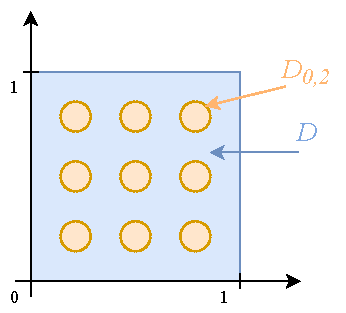
\includegraphics[width=0.5\textwidth]{figures/tensor_completion/CookieProblem.pdf}
  \caption{Illustration of Cookie problem with $m=3$ ($9$ cookies).}
  \label{fig:cookie_problem}
\end{figure}

The results of tensor completion are presented in Table~\ref{tab:results_cookie} (the variance of the initialization error for GP-based init is not presented as it is negligible in this case). One can see that GP-based initialization gives lower reconstruction errors both on the training set and test set except for ALS technique. ALS method with the proposed initialization
overfits: the error on the training set is close to $0$, whereas the test error is much more significant. The error on the training set is about $10^{-29}$, which means that the training set was approximated with machine precision.
It is not surprising if we recall that there are only $5000$ observed values, while the number of free parameters that are used to construct TT is much higher.

\subsubsection{CMOS ring oscillator}
\label{sec:cmos_ring_oscillator}
Let us consider the CMOS ring oscillator \citep{zhang2017big}. It is an electric circuit which consists of $7$ stages of CMOS inverters.
We are interested in the oscillation frequency of the oscillator. The characteristics of the electric circuit are described by $57$ parameters.
Each parameter can take one of $3$ values, so the total size of the tensor is $3^{57} \approx 1.57 \times 10^{27}$. The number of observed values that were used during the experiments is $N = 5000$. For the test set, we used $10000$ independently generated points.

The results of the experiments are given in Table~\ref{tab:results_cmos}. The table demonstrates that utilizing GP based initialization improves the results for all algorithms except ALS. ALS, in this case, overfits again: training error is extremely small, whereas the test error is much larger, though it is rather small compared to other techniques and ALS with random initialization.

\begin{table}[]
    \centering
    \caption{MSE errors for Cookie problem}
    \small
    \label{tab:results_cookie}
    \begin{tabular}{r|cc|cc|}
         & \multicolumn{4}{c|}{\textbf{Training set}} \\
         & \multicolumn{4}{c|}{$m = 3$} \\
        \hline
          & \multicolumn{2}{c|}{Random init} & \multicolumn{2}{c|}{GP init} \\
          & \multirow{2}{*}{error} & \multirow{2}{4em}{average N iters} & \multirow{2}{*}{error} &
          \multirow{2}{4em}{average N iters} \\
          & & & & \\
        \hline
        SGD & $(1.66 \pm 0.067) \times 10^{-2}$ & $1500$ &
        $\mathbf{(2.86 \pm 0.18) \times 10^{-5}}$ & $150$ \\
        Ropt & $(4.13 \pm 2.20) \times 10^{-8}$ & $1000$ &
        $\mathbf{(5.48 \pm 1.10) \times 10^{-10}}$ & $1000$ \\
        TTWopt & $(2.73 \pm 0.19) \times 10^{-4}$ & $100$ &
        $\mathbf{(9.21 \pm 2.17) \times 10^{-7}}$ & $100$ \\
        ALS & $(1.07 \pm 1.07) \times 10^{-4}$ & $100$ &
        $\mathbf{(2.39 \pm 0.60) \times 10^{-30}}$ & $100$ \\
        \hline
        Init error & $(1.15 \pm 0.24) \times 10^{8}$ &  &
        $\mathbf{2.66 \times 10^{-4}}$ &  \\
        \hline

        & \multicolumn{4}{c|}{$m = 4$} \\

        \hline
        SGD &
        $(3.14 \pm 1.08) \times 10^{-2}$ & $1500$ &
        $\mathbf{(1.65 \pm 0.13) \times 10^{-5}}$ & $150$ \\
        Ropt &
        $(1.42 \pm 0.01) \times 10^{-2}$ & $1000$ &
        $\mathbf{(3.42 \pm 0.50) \times 10^{-4}}$ & $1000$ \\
        TTWopt &
        $(1.31 \pm 0.00) \times 10^{-4}$ & $100$ &
        $\mathbf{(1.80 \pm 0.16) \times 10^{-6}}$ & $100$ \\
        ALS &
        $(6.59 \pm 3.30) \times 10^{-5}$ & $100$ &
        $\mathbf{(1.33 \pm 0.46) \times 10^{-29}}$ & $100$ \\
        \hline
        Init error & $(8.32 \pm 2.52) \times 10^{14}$ &  &
        $\mathbf{3.14 \times 10^{-4}}$ &  \\
        \hline

         & \multicolumn{4}{c|}{\textbf{Test set}} \\
         & \multicolumn{4}{c|}{$m = 3$} \\
         \hline

        SGD & $(2.06 \pm 2.31) \times 10^{-1}$ & --- &
        $\mathbf{(9.97 \pm 0.40) \times 10^{-5}}$ & --- \\
        Ropt & $\mathbf{(1.48 \pm 0.90) \times 10^{-7}}$ & --- &
        $(3.45 \pm 0.0165) \times 10^{-4}$ & --- \\
        TTWopt & $(4.52 \pm 0.50) \times 10^{-4}$ & --- &
        $\mathbf{(5.27 \pm 0.74) \times 10^{-6}}$& --- \\
        ALS & $\mathbf{(4.37 \pm 7.73) \times 10^{-2})}$ & --- &
        $(3.78 \pm 1.08) \times 10^{0}$ & --- \\
        \hline
        Init error & $(1.12 \pm 0.23) \times 10^{8}$ &  &
        $\mathbf{4.12 \times 10^{-4}}$ &  \\
        \hline


        & \multicolumn{4}{c|}{$m = 4$} \\

        \hline
        SGD & $(2.40 \pm 2.76) \times 10^{1}$ & --- &
        $\mathbf{(1.15 \pm 0.05) \times 10^{-4}}$ & ---\\
        Ropt & $(1.47 \pm 0.003 \times 10^{-2}$ & --- &
        $\mathbf{(5.38 \pm 0.07) \times 10^{-4}}$ & ---\\
        TTWopt & $(2.42 \pm 0.00) \times 10^{-4}$ & --- &
        $\mathbf{(3.02 \pm 0.17) \times 10^{-5}}$ & --- \\
        ALS & $\mathbf{(3.57 \pm 5.65) \times 10^{-1}}$ & --- &
        $(1.85 \pm 60.5) \times 10^{0}$ & ---\\
        \hline
        Init error & $(8.33 \pm 2.46) \times 10^{14}$ &  &
        $\mathbf{5.37 \times 10^{-4}}$ &  \\
        \hline


    \end{tabular}
\end{table}

\begin{table}[]
    \centering
    \caption{MSE errors for CMOS oscillator}
    \label{tab:results_cmos}
    \begin{tabular}{r|cc|cc|}
         & \multicolumn{4}{c|}{\textbf{Training set}} \\
        \hline
        & \multicolumn{2}{c|}{Random init} & \multicolumn{2}{c|}{GP init} \\
        & error & N iters & error & N iters \\
        \hline
        SGD & $(7.77 \pm 15.25) \times 10^5$ & $1500$ &
        $\mathbf{(3.11 \pm 4.87) \times 10^{-4}}$ & $150$ \\

        Ropt & $(6.22 \pm 0.01) \times 10^3$ & $1000$ &
        $\mathbf{(9.50 \pm 4.28) \times 10^{-5}}$ & $1000$ \\

        ALS & $(9.95 \pm 0.26) \times 10^{-2}$ & $300$ &
        $\mathbf{(3.57 \pm 0.45) \times 10^{-26}}$ & $300$ \\
        \hline
        Init error & $(1.67 \pm 3.19) \times 10^{12}$ & &
        $\mathbf{(3.95 \pm 2.19) \times 10^{-4}}$ & \\
        \hline

         & \multicolumn{4}{c|}{\textbf{Test set}} \\
        \hline

        SGD & $(3.45 \pm 9.68) \times 10^8$ & --- &
        $\mathbf{(4.65 \pm 5.01) \times 10^{-4}}$ & --- \\

        Ropt & $(6.23 \pm 0.0) \times 10^3$ & --- &
        $\mathbf{(9.68 \pm 4.16) \times 10^{-5}}$ & --- \\

        ALS & $(1.03 \pm 0.01) \times 10^{-1}$ & --- &
        $\mathbf{(4.09 \pm 3.10) \times 10^{-4}}$ & --- \\
        \hline
        Init error & $(1.04 \pm 2.53) \times 10^{15}$ & &
        $\mathbf{(3.90 \pm 2.15) \times 10^{-4}}$ & \\
        \hline
    \end{tabular}
\end{table}



All in all, the obtained results prove that GP-based initialization improves the tensor completion results in general. At least, it provides better training error. As for the error on the test set, one should be more careful as the number of degrees of freedom is large and there are many solutions that give a small error for the observed values but large errors for other values.



\subsection{Related work}
\label{sec:related_works}
% One of the most studied case is completion of $2$-, $3$- and $4$-dimensional tensors.
One set of approaches to tensor completion is based on nuclear norm minimization. The nuclear norm of a matrix is defined as a sum of all singular values of the matrix. This objective function is a convex envelope of the rank function. For a tensor, the nuclear norm is defined as a sum of singular values of matricizations of the tensor.

There are efficient off-the-shelf techniques for such types of problems that apply interior-point methods. However, they are second-order methods and scale poorly with the dimensionality of the problem. Special optimization technique was derived for nuclear norm minimization
\citep{gandy2011tensor, liu2013tensor, recht2010guaranteed,yuan2016tensor}.
However, calculation of the nuclear norm for tensors is a difficult task \citep{hillar2013most}
% (e.g. based on alternating direction method of multipliers \citep{gandy2011tensor},

% ADMM \citep{gandy2011tensor}

% \citep{liu2013tensor} --- weighted nuclear norm, block coordinate descent additional matrices $M$.
Some of the approaches involve solving large semi-definite programs \citep{barak2016noisy,potechin2017exact},
so they are infeasible when the dimensionality is high.
More often, such techniques are applied to matrices or
low-dimensional tensors as their straightforward
formulation allows finding the full tensor.
It becomes infeasible when we come to high-dimensional problems.


% There are several improvements \todo{elaborate, see smooth parafac}.

The second type of approaches is based on low-rank tensor decomposition \citep{acar2011scalable, chen2013simultaneous, kressner2014low, steinlechner2016riemannian, yuan2017completion}. There are several tensor decompositions, and all these papers derive some optimization procedure for one of them, namely, CP decomposition, Tucker decomposition
\citep{kolda2009tensor}, or TT/MPS decomposition. The simplest technique is the alternating least squares \citep{grasedyck2015alternating}.
It finds the solution iteratively at each iteration, minimizing the objective function w.r.t. one core while other cores are fixed.

Another approach is based on Riemannian optimization, which tries to find the optimal solution on the manifold of low-rank tensors of the given structure \citep{steinlechner2016riemannian}. The same can be done using Stochastic Gradient Descent \citep{yuan2017completion}. Riemannian optimization, TTWopt, ALS, and its modifications (e.g., ADF, alternating directions fitting \citep{grasedyck2013alternating}), try to find the TT representation of the actual tensor iteratively \citep{phien2016efficient,grasedyck2015variants}.
At each iteration, it optimizes TT cores such that the resulting tensor approximates well the tensor, which coincides with the real tensor at observed indices and with the result of the previous iteration at other indices. All these approaches need to specify rank manually.
In \citep{suzuki2015convergence,zhao2015bayesian} the authors apply the Bayesian framework for CP decomposition, which allows them to select the rank of the decomposition automatically.
The work \citep{yokota2016smooth} introduces smoothness constraints on PARAFAC decomposition to improve the results.

In some papers, the objective is modified by introducing special regularizers to suit the problem better \citep{yokota2016smooth}. For example, in \citep{chen2013simultaneous,zhao2015bayesian} to obtain better results for visual data, a special prior regularizer was utilized.
\citep{chen2017denoising} proposes a regularizer based on some specific matrix norm.
Many papers use total variation regularizer \citep{li2017low} for low-rank tensor completion.
The paper \cite{qin2020low} employs Shannon total variation as a regularization.

Our proposed algorithm is an initialization technique for the
tensor completion problems in TT format and can be used
with most of the algorithms solving such problems.
If the assumptions from Section~\ref{sec:tensor_completion_init} (the tensor values are values of some rather smooth function of tensor indices) are satisfied, the initial value will be close to the optimal,
providing better results.
The question of a good initialization is rarely considered.
In paper \citep{ko2018fast}, a special initialization is proposed for visual data. The idea is to use some crude technique (like bilinear interpolation) to fill missing values and after that, apply SVD-based tensor train decomposition.
The drawback of the approach is that it can be applied only in case of small-dimensional tensors, as we need to fill all missing values.
In \citep{grasedyck2013alternating}, they propose special initialization for the Alternating Direction Fitting (ADF) method.
This is a general technique for the tensor completion, and it does not consider the assumptions on the data generating function.



\section{Score Matching based on Random Features}
\label{sec:score_matching}

One of the core problems in statistics is a density estimation.
The most well-known approach is the Maximum Likelihood Estimation (MLE).
However, MLE and all other approaches based on MLE require normalizing constant to be known
or computed efficiently, which is not the case in many real world problems.
The intractability of the normalizing constant makes the approach infeasible.
In contrast, an unsupervised score matching estimator~\cite{Hyvarinen2005} based on Fisher divergence minimization, does not depend on the normalizing constant.
The resulting estimate is proved to be asymptotically normal and consistent in the case when
data and model distributions supports coincide.
There numerous developments of the
 idea~\cite{hyvarinen2007some, Lyu2012, Gutmann2012bregman, Kanti2016, dai2018kernel}.

Another important part of the density estimation is the class of models to search the solution in.
A special interest is paid here to an exponential family of distributions which leads to the
closed-form solution~\cite{hyvarinen2007some, forbes2015linear, Lin2016, Shiqing2018, monti2018}.
A generalization of the finite-dimensional exponential families is a kernel exponential family
(KEF).
In this case the natural parameter is treated a function from some
Reproducing Kernel Hilbert Space (RKHS).
It can be seen as infinite-dimensional generalization of the exponential family.
The KEF contains all well-known exponential family densities such as Exponential, Gaussian,
Gamma, etc.
In addition, RKHS reveals a sufficiently rich class of
estimators with convergence guarantees w.r.t. different
metrics~\cite{Gretton2013, Gretton2015}.
The main disadvantage is the computational cost for the sample matrix inversion making this
method inapplicable even for a moderate amount of the training data.

To approach the computational complexity issue~\cite{sutherland2017efficient, GrettonDeep} propose to use Nystr{\"o}m-type approximation of the kernel function.
Here we propose to use randomized feature maps as considered in
Chapter~\ref{chap:unstructured_datasets}.
Employing special structure on the discussed in Section~\ref{subsec:ortho}
we come up with a faster model than Nystr{\"o}-type approximation.
There are a lot of papers studying the convergence of the RFF models for the regression problem.
The optimal learning rate with $\mathcal{O}(\sqrt{n}\log n)$ features is the same as for the
full kernel \cite{aless2016generalization}
which gives substantial speed up.
The theoretical properties of using RFF for score matching is less studied,
though there are some general theoretical results on RFF and
higher order kernel derivatives~\cite{Orlicz,OperatorValuedKernels}.

Naive approach to score matching with random features suffer from several issues.
The first one is an oscillating behaviour in the tails of the distribution~\cite{Gretton2015}.
The second problem is poor convergence in the case of disjoint support
(consistency could not be guaranteed) or in the areas
where density value is close to zero~\cite{GrettonDeep}.
Inconsistency explains low approximation accuracy in regions of almost zero density.

It was shown that convolution with small Gaussian noise
(which is equivalent to the noisy data perturbation) improves learning behaviour and approximation
quality, e.g.~\cite{song2019generative,GANinstability, NoisyFGAN}.
It makes the support of both densities (distribution of the data and the model distribution)
the same and allows to overcome the aforementioned issue.
For most of the models the convolution cannot be calculated analytically,
so authors usually stick to the second-order Taylor series expansion
\cite{NIPS2010_4060, Reehorst_2019, NoisyFGAN} which results in a special
regularization term in the loss function.
It turns out that the noise level is an important parameter.
With large noise level we have better convergence but lower accuracy.
With smaller noise level the convergence is less stable, but the
solution is more accurate.
This means, that tuning of noise level is required.
Recently, it was proposed to use several noise levels optimizing
cumulative objective~\cite{song2019generative}.
% In this work we show, that for kernel exponential family we can find
% the optimal noise parameters by a simple gradient-based approach.


In this section we introduce method to estimate unknown distribution using
denoising score matching combined with random features.
To tackle the convergence issues we convolve the loss function with symmetric noise analytically.
It allows to avoid additional regularization terms as they are embedded into the loss function naturally.
The derived expression of the loss function explicitly contains the noise parameters
that allows us to use simple gradient-based approaches to tune these parameters.
In the experimental section we demonstrate the performance of our approach both in terms of
accuracy and training time.
While the quality is comparable to Nystr{\"o}m-type approximations, the training speed is much faster.


% The paper is organized as follows.
% In Section~\ref{sec:background} we give background information
% that is used to construct the final model:
% score-matching and its RKHS form, learning using random features.
% Section~\ref{chap:body} provides results on the necessary condition of denoising score matching
% and its RFF approximation.
% Numerical experiments are presented in Section~\ref{chap:experiments}.
% Finally, Section~\ref{chap:Conclusion} concludes the results of conducted research.
% All additional materials are presented in
% appendices~\ref{chap:Technical},~\ref{sec:B},~\ref{sec:C}.


\subsection{Score matching}
Let ${\cal D} = \{{\bf x}_a\}_{a = 1}^d, {\bf x}_a \in \mathbb{R}^d$ be a set of observations
drawn from an unknown distribution with a probability density function $p_0({\bf x})$.
Let $p({\bf x}, {\bm \theta})$ be a model density parameterized by
${\bm \theta} \in \Theta \subset \mathbb{R}^m$.
The task is to find such ${\bm \theta}^*$ that the model density is close to the real one:
$p({\bf x}, {\bm \theta}^*) \approx p_0({\bf x})$.
In score matching approach we minimize the Fisher divergence:
\begin{equation}
    J(p_0 \| p_{\bm{\theta}}) = \frac12 \int p_0({\bf x})\|\nabla \log p({\bf x}, {\bm \theta}) - \nabla \log p_0({\bf x})\|_2^2 d\bm{x}.
    \label{eq:fisher}
\end{equation}
Under sufficiently weak regularity conditions (see \cite{Hyvarinen2005})
the minimization of the Fisher divergence is equivalent to minimization of
\begin{equation}
    J(p_0 \| p_{\bm{\theta}}) \sim \mathbb{E}_{p_0}\left[\Delta \log p({\bf x}, {\bm \theta}) + \frac{1}{2}\|\nabla \log p({\bf x}, {\bm \theta})\|^2\right]
    \label{eq:fisher_sm}.
\end{equation}
Note, that the normalizing constant does not depend on ${\bf x}$,
therefore, $p({\bf x}, {\bm \theta})$ in \eqref{eq:fisher_sm}
could be replaced with unnormalized one
$\Tilde{p}({\bf x}, {\bm \theta}) = p({\bf x}, {\bm \theta}) Z({\bm \theta})$.
In an abuse of notation from now on we will use
$p({\bf x}, {\bm \theta})$ to denote the unnormalized density if it not stated explicitly.
% $\Tilde{p}({\bf x}, {\bm \theta})$ as .
Objective \eqref{eq:fisher_sm} now does not depend on unknown density $p_0$ and provides an
opportunity to estimate $p_0$ up to the normalizing constant using only samples drawn from $p_0$:
\begin{equation}
    \hat{J}(p_0 \| p_{\bm{\theta}}) = \frac{1}{n}\sum_{a = 1}^n\left[\Delta \log p({\bf x}_a, {\bm \theta}) + \frac{1}{2}\|\nabla \log p({\bf x}_a, {\bm \theta})\|^2\right] \to \min_{{\bm \theta}}.
    \label{eq:fisher_sm_sample}
\end{equation}
This loss suffers from several issues.
Firstly, the expression \eqref{eq:fisher} assumes that model and data distributions
have the same support.
However, in real world the real distribution lies on a low-dimensional manifold embedded
in $\mathbb{R}^d$ \cite{song2019generative},
while support of the model density is usually the whole space.
Secondly, score matching convergence is guaranteed only in the case of
${\rm supp\;} p_0 = \mathbb{R}^d$ (see \cite{Hyvarinen2005}).

To tackle the issue we use Denoising Score Matching (DSM) \cite{Denoising}.
In this approach we add noise to the data.
The score matching loss in this case is given by
\begin{equation}
    \label{eq:denoising_sm}
    DSM(p_{\bm{\theta}}) = \mathbb{E}_{p_{\varepsilon}}\mathbb{E}_{p_0}\left[\Delta \log p({\bf x} + {\bm \varepsilon}, {\bm \theta}) + \frac{1}{2}\|\nabla \log p({\bf x} + {\bm \varepsilon}, {\bm \theta})\|^2\right],
\end{equation}
where $p_{\varepsilon}(\bm{x})$ is a distribution of noise.
Now both densities have the same support, so the solution converges.
The optimal model satisfies
$\nabla p_{\bm{\theta}} = \nabla \left [p_0 * p_{\varepsilon} \right ] (\bm{x})$,
where $*$ is the convolution operator.
However, $\nabla \left [p_0 * p_{\varepsilon} \right ] (\bm{x})$ is
close to the true density $\nabla p_0(\bm{x})$
only when the noise is small enough.

To estimate the loss in general case we can generate finite set of
noisy samples and use them to estimate expectation in the loss function.
Another option is to use Taylor series expansion assuming that noise level is small.
In both cases we get approximate value of the loss function.
Moreover, when we use Taylor series expansion we need to calculate
higher order derivatives of the model which can be computationally complex
(for example, in case of neural networks).
However, for the kernel exponential family the denoising score matching loss
can be computed exactly.

\subsubsection{Kernel exponential family}
The kernel exponential family is a set of distributions where unnormalized
probability density functions
$p_f(\bf{x})$ satisfy
$\log p_f({\bf x}) = f({\bf x}) + \log q_0({\bf x})$,
$f \in \mathcal{H}$,
$\mathcal{H}$ is some Reproducing Kernel Hilbert Space (RKHS) with kernel $k$ and
$q_0$ is some generating density.
The normalizing constant is usually not known and cannot be computed analytically.
The class of such densities is rich enough.
In fact it is dense in a set of continuous probability density functions
that decay at the same rate as $q_0$.

In a well specified case, i.e. $p_0$ belongs to the kernel exponential family with RKHS
$\mathcal{H}$, the score matching loss \eqref{eq:fisher_sm}
can be expressed as (see \cite{Gretton2013})
\begin{equation}
    \label{eq:sm_kernel}
    J(p_0 \| p_f) =
    \frac{1}{2} \langle f, Cf\rangle_{\mathcal{H}} + \langle f, \xi\rangle_{\mathcal{H}} + J(p_0 \| q_0)
\end{equation}
where
$\partial^{\alpha,\beta}_{i, j + d} k({\bf x, \bf y}) =
\frac{\partial^{\alpha + \beta}}{\partial x_i^{\alpha}\partial y_j^{\beta}}k({\bf x, \bf y})$
and
\begin{align*}
    C &= \mathbb{E}_{p_0} \left[
        \sum_{i = 1}^d \partial_i k ({\bf  x}, \cdot) \otimes \partial_i k ({\bf  x}, \cdot)
    \right], \quad C \colon \mathcal{H} \to \mathcal{H} \\
    \xi &= \mathbb{E}_{p_0} \left[
        \sum_{i = 1}^d \partial_i k ({\bf  x}, \cdot)\partial_i \log q_0({\bf x}) +
        \partial^2_i k ({\bf  x}, \cdot)
        \right] \in \mathcal{H}.
\end{align*}

Using the general representer theorem the optimal $f({\bf x})$ can be found
as a weighted sum of the kernel derivatives located at the training samples.
To find the weights we need to invert $nd \times nd$ matrix and the computational
complexity, therefore, is $O(n^3d^3)$.
While the convergence in RKHS of this estimator implies the convergence in $L^r$,
in terms of Kullback-Leibler divergence and Hellinger distance,
in the misspecified case a density estimator remains the same,
but with convergence guarantees only for Fisher divergence.

To reduce complexity the authors of \cite{sutherland2017efficient} proposed to
find solution in a span over a randomly selected subset of training samples (inducing points).
The computational cost of this approach is $O(m^3d^3)$,
where $m$ is a number of inducing points.
Additional sub-sampling over $md$ basis functions enables even more computationally efficient
approach.
In this extreme case the complexity is $O(m^2nd + m^3)$.
As in the case of full data usage, obtained estimator is consistent when $p_0$
lies in the kernel exponential family,
but the rate of convergence is slower (under assumptions presented in \cite{sutherland2017efficient}).
The misspecified case was not studied.

To obtain consistent estimator from the kernel exponential family
the authors of \cite{GrettonDeep} used denoising score matching with Taylor series expansion.
This results in an additional regularization term in the loss function
that penalizes second derivatives of the model.
The need to calculate second derivatives restricts the approach only to
relatively low-dimensional cases.

%\newpage
\paragraph*{Random Features}
\label{sec:inrto_rff}
Random Features based approaches were discussed in Chapter~\ref{chap:unstructured_datasets}.
The difference in score matching problems is that
we work with the derivatives of the kernel function.
However, the same idea can be applied to the kernel derivatives
\begin{equation}
    \partial^{{\bf p}, {\bf q}} k({\bf x - y}) = \int p({\bf w}) \partial^{{\bf p}}\left[e^{j\bf{w^\top x}}\right]\partial^{{\bf q}}\left[e^{-j\bf{w^\top y}}\right]d\bf{w}
\end{equation}
where ${\bf p}, {\bf q} \in \mathbb{R}^d$ denote multi-indices,
$\partial^{\bf{p}} f =
\frac{\partial^{|\bf{p}_1 + \bf{p}_2 + \cdots + \bf{p}_d |} }{\partial x_1^{p_1} \ldots
\partial x_d^{p_d}} f$
and $\bf{p}$ and $\bf{q}$ act on the first and the second arguments of
the kernel correspondingly.
The theoretical properties of using random features are well studied only for the
kernel ridge regression \cite{aless2016generalization, li2018unified}.

\subsection{Kernel Denoising Score Matching}
\label{chap:body}
This section provides the optimal solution for the Kernel Denoising Score Matching,
its RFF approximation and some error bounds of the resulting model.
Here we assume that the noise distribution is symmetric, i.e.
$p_{\varepsilon}(\bf{x}) = p_{\varepsilon}(-\bf{x})$.

\subsection{Denoising Score Matching in RKHS}
We start from rewriting the expression for the Denoising Score Matching objective
\eqref{eq:denoising_sm}
and follow the same logic in derivation as in paper \cite{Gretton2013}
with the difference that our objective function is the convolution of the usual
score matching objective with noise distribution.

Let $V: \mathbb{R}^m \to \mathbb{R}$ be a convex and differentiable function.
Assume that the objective function takes the form
\[
    J(f) = V(\langle \phi_1, f\rangle_\mathcal{H},
             \langle \phi_2, f\rangle_\mathcal{H}, \ldots,
             \langle \phi_m, f\rangle_\mathcal{H}) + \frac{\lambda}{2}\|f\|^2_\mathcal{H},
\]
for any set $\{\phi_i(\cdot)\}_{i = 1}^m$, $\phi_i \in \mathcal{H}$.

For our case we define the set of functions $\{\phi_i(\cdot)\}$ as follows
\begin{align*}
    &\phi_{(a - 1)d + i}(\cdot) = \partial_i k({\bf x}_a + {\bf y}, \cdot),\\
    &\phi_{nd + 1}(\cdot) = \frac{1}{n}\sum\limits_{a, i = 1}^{n, d} \partial_i^2 k({\bf x}_a + {\bf y}, \cdot) + \partial_i k({\bf x}_a + {\bf y}, \cdot)\partial_i \log q_0({\bf x}_a + {\bf y}),
\end{align*}
and for simplicity let us denote it as $\{\phi_i(y, \cdot)\}_{i = 1}^m$, $m = nd + 1$.
Now let us define a linear operator
$A({\bf y}): \mathcal{H} \to \mathbb{R}^m$, $f \to \{\langle\phi_i({\bf y}, \cdot),
f\rangle_\mathcal{H}\}_{i = 1}^m$.
Then the objective \eqref{eq:denoising_sm} can be written as
\begin{equation}
    \label{eq:denoising_objective_rkhs}
    f^* = \argmin_{f \in \mathcal{H}} \int p_{\varepsilon}({\bf y})V(A({\bf y})f)d{\bf y}
    + \frac{\lambda}{2}\|f\|^2,
\end{equation}
with $V(\theta_1, \ldots, \theta_{nd + 1}) =
\frac{1}{2n}\sum\limits_{a = 1}^n\sum\limits_{i = 1}^d\theta^2_{(a - 1)d + i} +
\theta_{nd + 1}$.

Using the first order optimality condition we can see that the solution takes the form
\[
    f = \int p_{\varepsilon}({\bf y})A^*({\bf y}){\bm \alpha}({\bf y})d {\bf y},
    \quad
    {\bm \alpha}({\bf y}) = -\frac{1}{\lambda}\nabla V(A({\bf y})f),
\]
where $A^*({\bf y}): \mathbb{R}^m \to \mathcal{H}$ is an adjoint to $A({\bf y})$.
% and
% $A^*({\bf y}){\bm \alpha} = \sum_{i = 1}^m \alpha_i\phi_i({\bf y}, \cdot)$, denoting
% \[
%     {\bm \alpha}({\bf y}) = -\frac{1}{\lambda}\nabla V(A({\bf y})f),\quad f = \int p_{\varepsilon}({\bf y})A^*({\bf y}){\bm \alpha}({\bf y})d {\bf y}
% \]
% first order optimality condition could be written as an integral equation on ${\bm \alpha}({\bf y})$:
% \begin{equation}
%     {\bm \alpha}({\bf y}) = -\frac{1}{\lambda}\nabla V\left(\int p_{\varepsilon}({\bf z})A({\bf y})A^*({\bf z})\alpha({\bf z})d{\bf z}\right)
% \end{equation}
% where $A({\bf y})A^*({\bf z})\alpha({\bf z}) = \sum\limits_{i = 1}^m\alpha_i({\bf z})\{\langle \phi_j({\bf y}, \cdot),  \phi_i({\bf z}, \cdot)\rangle\}_{j = 1}^m = {\bm K}({\bf y}, {\bf z}){\bm \alpha}({\bf z})$.
Now we are ready to formulate the proposition.
\begin{proposition}
    The solution to \eqref{eq:denoising_objective_rkhs} has the following form
    \[
        f^* = B \left [
            -\frac{1}{n\lambda}C(\bm{\beta}^*) + \frac{1}{n\lambda^2}b
        \right ],
    \]
    where
    $\hat{A}({\bf y}) \colon \mathcal{H} \to \mathbb{R}^{m - 1}$,
    $\left ( \hat{A}({\bf y})f \right )_i = \left( A(\bf{y})f \right )_i, i=1, \ldots, m-1$,
    \newline
    $B = \int p_{\varepsilon}({\bf y})\hat{A}^*({\bf y})\hat{A}({\bf y}) d{\bf y}$,
    $b = \int p_{\varepsilon}({\bf y})\phi_m({\bf y}, \cdot) d {\bf y}$,
    $C(\bm{\beta}) = \int p_{\varepsilon}({\bf x})\hat{A}({\bf y})\bm{\beta}({\bf y})d{\bf y}$
    and ${\bm\beta}^*({\bf y})$ is the solution to
    \begin{equation}
        \bm{\beta}({\bf y}) = -\frac{1}{n\lambda}
        \int p_{\varepsilon}({\bf z}) \hat{A}({\bf y})\hat{A}({\bf z})^*\bm{\beta}({\bf z})
        d{\bf z}
        + \frac{1}{n\lambda^2}
        \int p_{\varepsilon}({\bf z}) \hat{A}({ \bf y}) \phi_m({\bf z}, \cdot)d{\bf z}.
    \label{eq:beta_integal}
    \end{equation}
\end{proposition}
See the details on derivation in \ref{sec:exact_solution}.

The optimal model requires solution of operator equation and in general
this is a difficult task.
In order to avoid this, let us consider a Monte-Carlo approximation
of~\eqref{eq:beta_integal}.
Suppose we sampled $K$ noise vectors $\{{\bf z}_k\}_{k = 1}^K$,
${\bf z}_k \sim p_{\varepsilon}$.
In this case the approximation to the optimal ${\bm \beta}^*$ can be found
by solving the system of equations
\begin{equation}
    \label{eq:beta_finite_sample}
    {\bm \beta}_K({\bf y}) = -\frac{1}{nK\lambda}
    \sum\limits_{k = 1}^K
    \hat{A}({\bf y})\hat{A}({\bf z}_k)^*{\bm \beta}_K({\bf z}_k)
    + \frac{1}{n\lambda^2}\int p_{\varepsilon}({\bf z}) \hat{A}({\bf y}) \phi_m({\bf z}, \cdot)d{\bf z}.
\end{equation}
The obtained result can then be used to derive an approximation of $f^*$,
but the computational complexity is $O(n^3d^3K^3 + n^2d^2K)$.
Moreover, the convolution in the second term of \eqref{eq:beta_finite_sample} could be directly computed
only for a limited set of kernels, e.g. Radial Basis Function kernel (RBF).

In order to improve the computational complexity we employ RFF approach
to the kernel function approximation.

\subsubsection{RFF for Denoising Score Matching}
For the RFF \eqref{eq:bochner}
we introduce the following matrix of RFF derivatives $\partial {\bm \Phi}_y$
corrupted by noise $\bf{y}$.
The $((a - 1)d + i)$-th row of matrix $\partial {\bm \Phi}_y$ is given by
$[\partial \bm{\Phi}_y]_{(a - 1)d + i} = \partial_i \bm{\phi}^\top(\bm{W}({\bf x}_a + \bf{y}) + \bm{b})$,
where $\partial_i \bm{\phi}^\top(\bm{W}({\bf x}_a + \bf{y}) + \bm{b})$
is an element-wise partial derivative of the feature vector at point ${\bf x}_a$.
Similarly, for the second derivatives we have
$[\partial^2 \bm{\Phi}_y]_{(a - 1)d + i} =
\partial^2_i \bm{\phi}^\top(\bm{W}({\bf x}_a + \bf{y}) + \bm{b})$.
The finite sample solution to \eqref{eq:beta_finite_sample} is given by
\[
    f_K
    = \frac{1}{n\lambda^2}{\bm \phi}(\cdot)^{\top}{\bm H}
    \left[-\frac{1}{K}\left(\frac{1}{K}\partial  {\bm \Phi}_K^{\top}\partial{\bm \Phi}_K + n\lambda {\bf I}\right)^{-1}\partial {\bm \Phi}_K^{\top}\partial{\bm \Phi}_K \odot {\bm h} + {\bm h}\right]
    -\frac{1}{\lambda} {\bm \phi}(\cdot)^{\top}{\bm h}.
\]
Here operator $\odot$ denotes the Hadamard product.
Let us denote
\begin{equation}
    \label{eq:h}
    {\bm H} = \int p_{\varepsilon}({\bf y})\partial{\bm \Phi}_y^{\top}\partial{\bm \Phi}_y
    d{\bf y},
    \quad
    {\bm h} = \frac{1}{n}(\partial^2 {\bm \Phi}_z * p({\bf z}))^{\top}{\bf 1}.
\end{equation}
Then by taking limit over $K \to \infty$ we obtain the final RFF solution
\begin{equation}
\label{eq:rff_f}
    f_{m}^* = \lim\limits_{K \to \infty} f_K
    = \frac{1}{\lambda}{\bm \phi}(\cdot)^{\top}({\bm H} + n\lambda{\bf I})^{-1}{\bm Hh}
    - \frac{1}{\lambda}{\bm \phi}(\cdot)^{\top}{\bm h}.
\end{equation}
The detailed derivation can be found in \ref{sec:rff_solution_derivation}.

Similar result can be derived for the Nystr\"om-type approximation
(see \ref{sec:Nystrom}).
The disadvantage in this case is that we need to calculate
convolution of the first and second order derivatives with the noise distribution
for each kernel.
For RFF, on the other hand, all the terms remains the same for any shift-invariant kernel
except the distribution of weights $\bf{W}$, which is much more convenient.

Another important thing we would like to stress is that in the resulting solution
each feature has a weight proportional to
$\exp \left ( -\frac{\sigma^2}{2} \|{\bf w}_i\| \right )$
(see \ref{sec:rff_solution_derivation} for details).
This means that the high-frequency features have weight which is close to zero.
Such behaviour can be interpreted as a regularization that penalizes
oscillating terms.

There are several hyper-parameters in the approach that affects the resulting
quality, namely, the kernel hyper-parameters ${\bm \theta}$,
the regularization parameter $\lambda$ and,
assuming that the noise is zero-mean Gaussian, the noise variance $\sigma$.
To tune these parameters we use the loss on the hold-out (validation) set.
The loss in this case is ordinary score matching (no denoising) loss as we would like to estimate
how good our model approximates the original data, not the noisy one.

Another important part of the algorithm is the base density $q_0$.
From a theoretical point of view, base density is responsible for the tails of the
distribution and do not affect the estimator in the areas with high density.
Therefore, in this section we consider three different options for $q_0$:
uniform distribution with support bounded by particular training sample,
multivariate Gaussian distribution and the mixture of Gaussians.
In the latter case, $q_0$ is fitted before training using Bayesian Mixture Model \cite{bishop}.

At the end of the training we estimate the normalizing constant via importance sampling
as was proposed in \cite{GrettonDeep}.
It should be noted that in the case of uniform base density normalization could not be
estimated properly due to the unknown data support measure.
The whole method is summarized in Algorithm \ref{alg:KDSM}.
\begin{algorithm}
\caption{Kernel denoising score matching.}
\label{alg:KDSM}
\begin{algorithmic}[1]
    \Require Training set ${\cal D}$, $m$~--- number of Fourier features,
    $n_z$~--- number of samples to estimate normalization constant,
    initial regularization parameter $\lambda$
    \State Fit $q_0({\bf x})$ to the given data set.
    \While{not stopping condition}
        \For{mini-batches ${\cal D}_t, {\cal D}_v \in {\cal D}$}
            \State Compute random Fourier approximation $f_m^*$ using equation \eqref{eq:rff_f} on ${\cal D}_t$.
            \State Compute ordinary score matching loss on validation
            \[
                \hat{J}_{val}(\lambda, \sigma, {\bm p}_k) =
                \frac{1}{|{\cal D}_v|}\left[
                    {\bf 1}^{\top}\partial^2 \bm{\Phi}_{v}\bm{b}_t +
                    \frac{1}{2}\bm{b}_t^{\top}\partial \bm{\Phi}_{v}^{\top}
                    \partial \bm{\Phi}_{v}\bm{b}_t +
                    \bm{b}_t^{\top}\partial \bm{\Phi}_{v}^{\top} \nabla\log q_0({\bf x})
                \right]
            \]
            \State Do gradient step over hyper-parameters ($\lambda$, $\sigma$, ${\bm p}_k$)
        \EndFor
    \EndWhile
    \State Compute $f_m^* = \bm{\phi}(\cdot)^{\top}\bm{b}_{\cal D}$
    using full dataset ${\cal D}$
    \State Compute normalization constant approximation $\hat{Z}$ via importance sampling
    \[
        \hat{Z} = \frac{1}{n_z}\sum_{i = 1}^{n_z}\frac{f_m^*({\bf x}_i)}{q_0({\bf x}_i)},
        \quad {\bf x}_i \sim q_0({\bf x})
    \]
\end{algorithmic}
\Return $\log p_f = f_m^* - \hat{Z}$
\end{algorithm}


The total complexity of the proposed approach is $O(m^3 + nm^2 + nmd)$,
where $O(nmd)$ operations are required generate random features,
$O(nm^2)$ is to compute feature matrix ${\bm H}$
and $O(m^3)$ corresponds to the matrix inversion which can be reduced to
$O(m^2)$ in some cases by using iterative methods for solving systems of linear equations.

Now, let us provide the bounds on the error of the approximation of the proposed approach.
Let us introduce the derivatives of the exact kernel matrix
\[
    \partial^p\partial^q {\bm K}_{(a - 1)d + i, (b - 1)d + j} = \partial^p_i\partial^q_{d + j}k({\bf x}_a, {\bf x}_b),
    \quad
    p, q \in \mathbb{N}_+.
\]
We also denote the derivatives of the random feature vector as
\[
   \partial^p\bm{\phi} = \begin{pmatrix}
        \partial_1^p\bm{\phi}({\bf w}^{\top}{\bf x}_1 + b) &
        \cdots &
        \partial^p_d\bm{\phi}({\bf w}^{\top}{\bf x}_n + b)
   \end{pmatrix}^\top.
\]
The error bounds for score matching with RFF is given by the following theorem.
\begin{theorem}
    Let $\delta \in (0, 1)$, $\varepsilon > 0$, then for
    $n \geq \frac{8}{3\varepsilon^2} \log\frac{m}{\delta}$ and assuming that
    ${\bf D}_1 = \mathbb{E}_{\bf w}{\rm tr}[\partial\bm{\phi}\partial\bm{\phi}^{\top}]
    \partial\bm{\phi}\partial\bm{\phi}^{\top} < \infty$, ${\bf D}_2 =
    \mathbb{E}_{\bf w}{\rm tr}[\partial^2\bm{\phi}\partial^2\bm{\phi}^{\top}]\partial\bm{\phi}
    \partial\bm{\phi}^{\top} < \infty$,
    we have that with probability at least $(1 - \delta)$ the following upper bound
    on distance between an averaged RFF score matching solution $f_{n, m}^*$
    and exact kernel solution $f_n^*$ holds
    \begin{align*}
        \mathbb{E}_{{\bf x}, {\bf w}}(f_{n, m}^*({\bf x}) - f_n^*({\bf x}))^2 \leq
        \frac{2}{\lambda^2 n^2 m^2}\left[
            \vphantom{\partial\partial {\bm K}^{\frac{1}{2}}} \right .
            & m\|\partial\partial {\bm K}^{\frac{1}{2}}(\partial\partial {\bm K} + \lambda n{\bf I})^{-1}\partial\partial^2 {\bm K}{\bf 1}\|^2 +\nonumber \\
            &m{\bf 1}^{\top}\partial^2\partial^2{\bm K}{\bf 1} +
            (1 + \varepsilon m)\|{\bf D}_2^{\frac{1}{2}}{\bf 1}\|^2 + \nonumber \\
            &\left . (1 + \varepsilon m)\|{\bf D}_1^{\frac{1}{2}}(\partial\partial {\bm K} + \lambda n {\bf I})^{-1}\partial\partial^2 {\bm K}{\bf 1}\|^2
        \right ].
    \end{align*}
\end{theorem}
The proof of the theorem is given in \ref{sec:error_bound_proof}.

\subsubsection{Discussion}

While RFF kernel approximation admits computationally efficient solution of score matching,
the convergence properties remains an open question.
Using results from \cite{Gretton2013} the convergence can be established only in the
RKHS that corresponds to the approximate kernel.
So we have the following relation
\[
    J(p_0\| p_{\lambda, n, m}) \to \inf_{p \in \Tilde{{\cal P}}}J(p_0\| p)
    \quad
    \lambda \to 0,~\lambda n \to \infty,~n \to \infty,
\]
where $p_{\lambda, n, m}$ is the density obtained using $m$ features and
$\Tilde{{\cal P}}$ is an exponential family with sufficient statistic
$\phi({\bm W}{\bf x} + {\bm b})$.
To upper bound the error of the approximation we
can consider the following inequality
\[
    \|f_{\lambda, n, m} - f_0\| \leq
        \|f_{\lambda, n, m} - f_{\lambda, m}\| +
        \|f_{\lambda, m} - f_{\lambda}\| +
        \|f_{\lambda} - f_0\|,
\]
where $f_{\lambda}$ minimizes \eqref{eq:sm_kernel} and
$f_{\lambda, n}$ is a solution of a finite sample version of \eqref{eq:sm_kernel},
$\|\cdot\|$ is a norm in $L^2({\mathbb{R}^d}, p_0)$.
$\|f_{\lambda,n, m} - f_{\lambda, m}\|$ includes the term $\|\hat{\xi}_m - \hat{\xi}\| = O(m^{-\frac{1}{2}})$ that can obtained using concentration lemma from
\cite{sutherland2017efficient} under additional assumption on the boundness
of the derivatives of the approximate kernel.
This implies that we should potentially use $O(n)$ features to obtain the same
convergence rates as in the case of exact solution.
To reduce the lower bounds on number of features
we need to provide refined analysis in a way similar to
\cite{aless2016generalization, li2018unified} in the future study.

In the case of Denoising Score Matching the estimated density will converge to the
$p^* * p_{\varepsilon}$, where $p^* = \inf_{p \in \Tilde{{\cal P}}}J(p_0\| p)$
is the density from $\Tilde{\mathcal{P}}$ closest to $p_0$.
So, on one hand the noise variance should be as small as possible.
On the other hand, the Wasserstein distance
between the approximation and the true density for the
Denoising Score Matching can be upper bounded as follows
\[
    W(p_0, p) \leq
    \mathbb{E}[\|{\bm \varepsilon}\|^2]^{\frac{1}{2}} +
    \tilde{C}\sqrt{J(p_0 * p_{\varepsilon}, p_{\lambda, n, m} * p_{\varepsilon})},
\]
where $\mathbb{E}[\|{\bm \varepsilon}\|^2] = n\sigma^2$.
The second term takes large value for small noise levels (due to different supports
of the approximate density and the true density)
and smaller values for large noise values.
So the choice of $\sigma$ is a trade-off between estimator stability and
how close it is to the unknown density function $p_0$.


\subsection{Results}
\label{chap:experiments}
\subsubsection{Experimental setup}
In all our experiments we used RBF kernel with diagonal covariance matrix,
the noise was assumed to be isotropic Gaussian (though in general
we can use arbitrary noise covariance matrix).

We compare the proposed approach (DSM RFF),
ordinary score matching with RFF (SM RFF),
exact kernel solution \eqref{eq:sm_kernel} (Exact) and
its Nystr\"om version with subsampled basis \cite{sutherland2017efficient} (Nystr\"om).
We used original implementations of this model from \cite{GrettonGit}.

The comparison is conducted on two types of data: artificially generated 2D densities
and datasets from the UCI repository \cite{UCI}
(the particular choice of data is motivated by previous research on kernel exponential family
\cite{sutherland2017efficient, Gretton2015, GrettonDeep}):
\begin{enumerate}
    \item Synthetic data generated from the following densities: a mixture of Gaussians, Uniform, Mixture on Uniforms, Cosine, Funnel, Banana, Ring, Mixture of Rings.
    \item RedWine, WhiteWine, MiniBoone.
\end{enumerate}
The Exact kernel model was not compared on MiniBoone dataset
because it's too computationally expensive.

To estimate the quality of models the following metrics were used:
\begin{enumerate}
    \item Log-likelihood (higher is better).
    It requires the normalization constant which can only be approximated, so
    the log-likelihood tends to be overestimated \cite{GrettonDeep}.
    \item Fisher divergence (lower is better).
    It requires true log-density gradient to be known and hence could be estimated only for
    artificial data, moreover, for uniform settings could be computed only on the support of
    true density.
    Alternatively, score-matching could be used, but scores for different models
    are not comparable in general.
    \item Finite-Set Stein Discrepancy (FSSD) goodness of fit test \cite{FSSD, GOF} with $0.05$
    significance level.
    We used Gaussian kernel, and its lengthscale was chosen to be median over
    pairwise distances between samples in order to avoid optimization over test points for the
    particular model, otherwise, we can not compare models.
    FSSD statistic almost surely equals to zero if and only if model density and $p_0$
    coincide.
    \item Wasserstein distance.
    In order to estimate this quantity, we used Metropolis Adjusted Langevin Algorithm (MALA)
    \cite{MALA} to draw samples from the model densities.
    We used step-size $0.1$, chain length was $10^4$ with $5\cdot 10^3$ burn-in.
\end{enumerate}

\subsection{Results}

We start by considering an approximate denoising approach (see \ref{sec:Taylor} for derivation)
to figure out if there is a benefit from the convolution with noise.
To accomplish this we construct illustrative experiment with $300$ RFF
features for Gaussian mixture.
We used multivariate Gaussian distribution for $q_0$
and the training set size was $10^3$.
The results are presented on Fig.~\ref{fig:demo},
from which it is clear that noisy approach better estimates ground truth in between components
region even with the presence of small noise
Also note the that there are less oscillations when we add noise to the data.
\begin{figure}[!ht]
  \centering
  \begin{subfigure}[b]{0.32\textwidth}
    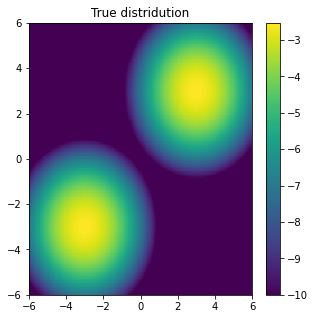
\includegraphics[width=\textwidth]{figures/score_matching/exps/taylor_MoG_true.png}
    \captionsetup{justification=centering}
    \caption{Ground truth\\ \hfill}
    \label{sfig:MoGtrue}
  \end{subfigure}
  \begin{subfigure}[b]{0.32\textwidth}
    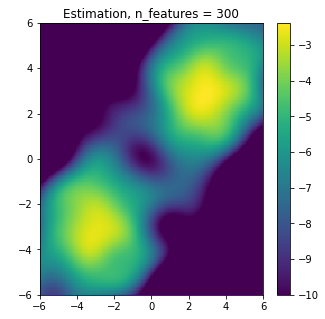
\includegraphics[width=\textwidth]{figures/score_matching/exps/taylor_MoG.png}
    \captionsetup{justification=centering}
    \caption{RFF, no noise, $SM~=~-0.68$}
    \label{sfig:MoGrff}
  \end{subfigure}
  \begin{subfigure}[b]{0.32\textwidth}
    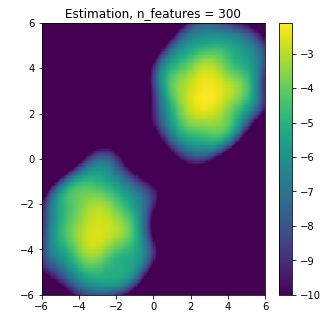
\includegraphics[width=\textwidth]{figures/score_matching/exps/taylor_MoG_noise_1.png}
    \captionsetup{justification=centering}
    \caption{RFF+noise, $SM~=~-0.99$}
    \label{sfig:MoGnoise}
  \end{subfigure}
  \begin{subfigure}[b]{0.32\textwidth}
    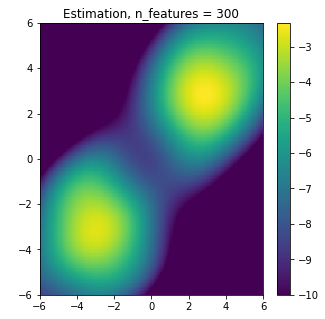
\includegraphics[width=\textwidth]{figures/score_matching/exps/MOG_rff.png}
    \captionsetup{justification=centering}
    \caption{RFF, no noise, wide kernel, $SM~=~-0.49$}
    \label{sfig:MoGrff_1}
  \end{subfigure}
  \begin{subfigure}[b]{0.32\textwidth}
    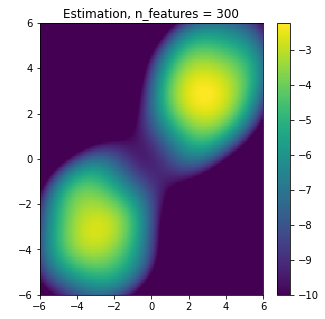
\includegraphics[width=\textwidth]{figures/score_matching/exps/MOG_noise.png}
    \captionsetup{justification=centering}
    \caption{RFF+noise, wide kernel, $SM~=~-0.67$}
    \label{sfig:MoGnoise1}
  \end{subfigure}
  \caption{Comparison of score-matching with and without noise,
    noise variance is
    $\sigma = 5\cdot10^{-4}$.
    We clip values of log-density that less then $-10$.
  }
  \label{fig:demo}
\end{figure}

The next step is to compare the proposed algorithm to other approaches on synthetic 2D data
and datassets from UCI.
In this case we used $512$ Random Fourier Features.
As the base density $q_0$ we used mixture of Gaussians.
As in the previous example a relatively small sample size was used.
Our models were trained for $60$ iterations using Adam optimizer with $0.1$ learning rate,
$512$ features were used.


% The results for Cosine and mixture of uniforms are presented
% in Figure~\ref{fig:2d_1000} (other results can be find in \ref{sec:C}).


For cosine data the form of distribution estimated via DSM RFF is much closer
to the real one.
However, for the mixture of uniforms it fails to correctly estimate weights
of the components.
In both of this densities, we observe model misspecification in the case of SM RFF
because all other 2D densities have full space support.
For the rest distributions there is no significant visual difference.
\begin{figure}[!ht]
    \centering
    \begin{subfigure}[b]{\textwidth}
      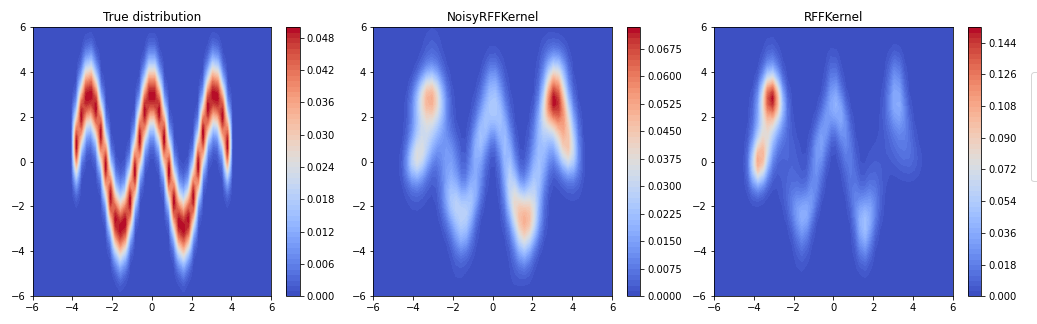
\includegraphics[width=\textwidth]{figures/score_matching/2D/Cosine1000.png}
      \caption{Cosine}
      \label{sfig:1000Cos}
    \end{subfigure}
    \begin{subfigure}[b]{\textwidth}
      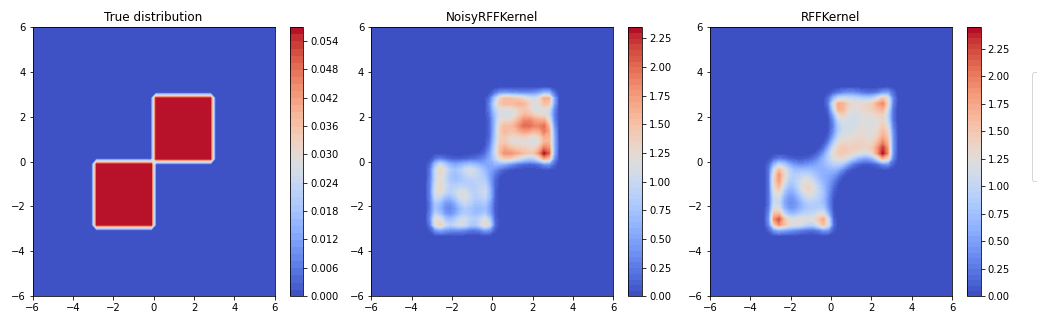
\includegraphics[width=\textwidth]{figures/score_matching/2D/Mixture1000.png}
      \caption{Mixture of uniforms}
      \label{sfig:1000Rings}
    \end{subfigure}
    \caption{Density estimates using DSM RFF (middle column) and SM RFF (right column).
    The ground truth density is in the first column.
    }
    \label{fig:2d_1000}
\end{figure}

These experiments showed that denoising score matching with RFF
in general works better for distributions with bounded support.
For the multimodal distributions it could fail to correctly estimate weights of
components or oversmooth the areas between components.
\begin{figure}[!ht]
  \centering
  \begin{subfigure}[b]{0.32\textwidth}
    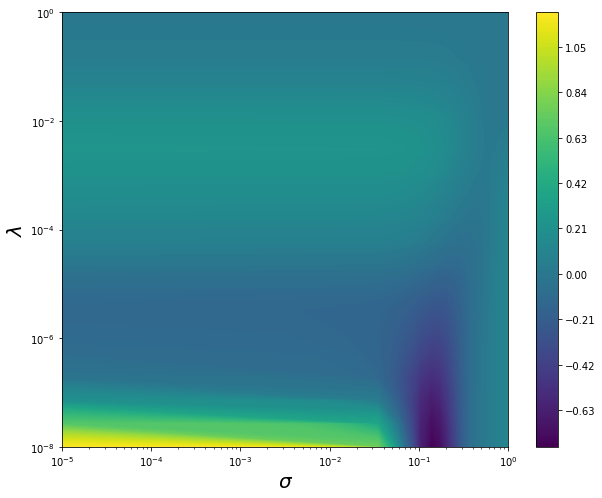
\includegraphics[width=\textwidth]{figures/score_matching/loss/lossUniform.png}
    \caption{Uniform}
  \end{subfigure}
  \begin{subfigure}[b]{0.32\textwidth}
    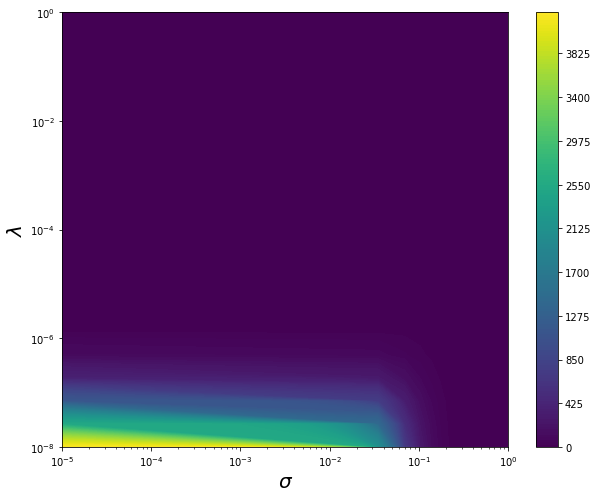
\includegraphics[width=\textwidth]{figures/score_matching/loss/lossFunnel.png}
    \caption{Funnel}
  \end{subfigure}
  \begin{subfigure}[b]{0.32\textwidth}
    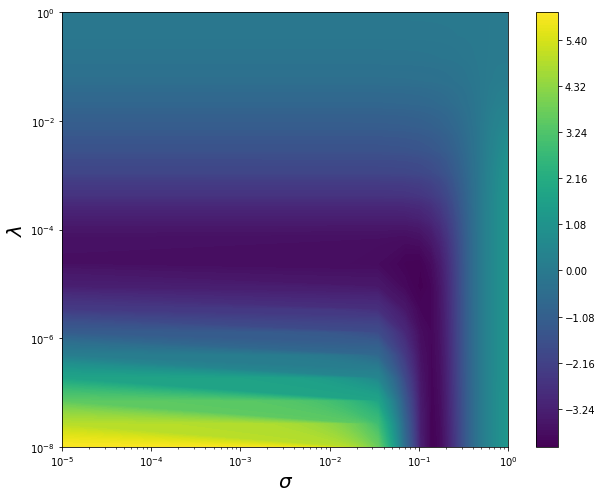
\includegraphics[width=\textwidth]{figures/score_matching/loss/lossRings.png}
    \caption{Two Rings}
  \end{subfigure}
  \caption{Dependence of loss on the regularization parameter $\lambda$ (y axis) and noise $\sigma$ (x axis).}
  \label{fig:lossdemo}
\end{figure}
Another observation about the approach is that in some cases it tends to choose
large noise variance.
In Fig.~\ref{fig:lossdemo} we visualize the dependence of the loss on
the regularization parameter and noise variance for several 2D distributions.
Interestingly, for "good" distributions
(like Funnel, that have full space support and one mode) the loss surface has wide
minimum w.r.t regularization and noise variance.
For multimodal distributions the loss surface has narrower minimum.
For uniform distribution (which differs from other that it has bounded support)
the minimum w.r.t noise variance is narrow but it is also separated from zero.
This indicates the need for the noise in such cases.


% In order to compare with exact kernel models, let us consider uniform base model, $10^4$ sample size and $512$ features (in the case of Nystr\"om estimator it is better to say components), the choice of relatively small sample size is caused by $O(n^2d^2)$ space complexity of the full kernel approach. In order to compare results for these model random search of hyperparameters was used. From the above experiments, the densities of interest are cosine, uniform, ring and the mixture of rings. Quantitative results are presented in the table~\ref{tab:RFFvsGretton}. While exact kernel models outperform in three of four cases in terms of Fisher divergence, for uniform distribution according to the $p$-value of FSSD test the hypothesis that $p_f = p_0$ is rejected for both exact kernel and Nystr\"om estimators. However, DSM RFF is comparable with them in Wasserstein distance.

% \begin{table}[!ht]
%     \centering
%     \begin{tabular}{llrrrrr}
% \toprule
% Distribution &           Model &  F$_{train}$ &  F$_{test}$ &   FSSD &  p-value & W1 \\
% \midrule
%     \multirow{2}{*}{Cosine}
%             &       DSM RFF &          6.783 &         6.458 &  0.040 &    0.300 &  \textbf{0.211} \\
%             &       SM RFF &          7. &         6.689 &  0.085 &    0.251 &  0.232 \\
%             &       Exact &          \textbf{3.656} &         \textbf{3.558} &  0.260 &    0.148 &  \textbf{0.17} \\
%             &       Nystr\"om &          \textbf{3.658} &         \textbf{3.561} &  0.261 &    0.147 &  0.35 \\
%             \hline
%     \multirow{2}{*}{Uniform}
%             &       DSM RFF &          1. &         1.171 &  0.130 &    0.116 &  \textbf{0.059} \\
%             &       SM RFF &         1.062 &         1.308 &  0.138 &    0.122 &  0.141 \\
%             &       Exact &          \textbf{0.7} &         \textbf{0.811} &  0.338 &    0.004 &  0.513 \\
%             &  Nystr\"{o}m &          \textbf{0.7} &         \textbf{0.81} &  0.342 &    0.004 &  \textbf{0.065} \\
%             \hline
%     \multirow{2}{*}{Ring}
%             &       DSM RFF &          \textbf{0.394} &         \textbf{0.392} & -1.899 &    0.908 &  \textbf{0.06} \\
%             &            SM RFF &          \textbf{0.436} &         \textbf{0.430} & -1.805 &    0.901 &  0.139 \\
%             &                Exact &          0.998 &         0.883 &  0.841 &    0.240 &  \textbf{0.55} \\
%             &  Nystr\"{o}m &          0.998 &         0.884 &  0.827 &    0.241 &  0.688 \\
%             \hline
%     \multirow{2}{*}{Rings}
%             &       DSM RFF &          \textbf{2.027} &         \textbf{1.97} & -0.466 &    0.703 &  \textbf{0.42} \\
%             &            SM RFF &          3.115 &         2.856 & -0.863 &    0.872 &  0.436 \\
%             &                Exact &          \textbf{2.352} &         \textbf{2.376} & -0.223 &    0.512 &  \textbf{0.394} \\
%             &  Nystr\"{o}m &          2.353 &         2.378 & -0.223 &    0.512 &  0.438 \\
% \bottomrule
% \end{tabular}
%     \caption{Comparison of score matching approached with exact kernel solution and its Nystr\"{o}m-type approximation on synthetic data \cite{Gretton2013, sutherland2017efficient}.}
%     \label{tab:RFFvsGretton}
% \end{table}


In Figure~\ref{fig:metrics} we plot all the metrics for all data sets.
For each dataset each metric was normalized across methods to have unit norm.
This was done only for better visualization.
The original values are given in \ref{sec:B}.
The figure illustrates the mean value of the metrics and corresponding variance
calculated across $10$ runs.
From the figure we can see, that w.r.t. almost all metrics (except the log-likelihood)
the proposed approach shows better or comparable results in many cases.
Actually, the Wasserstein distance is smaller for DSM RFF for all data sets.
We can also see, that SM RFF tends to have larger variance than its noisy version.

In Table~\ref{tab:metrics} we provide results for the datasets from the UCI repository
as well as the training time.
The MiniBoone dataset is large and the Nystr\"om-based implementation
could not fit into memory, so we had to train the model using only a subset of
$15000$ samples.
Other methods were trained using the whole data set.
To fairly compare the training time the experiments were conducted on
Intel(R) Core(TM) i7-7820X CPU @ 3.60GHz with 64Gb RAM.
We can see that the proposed approach is much faster than the implementation
of the Nystr\"om based approach.


\begin{figure}[h]
  \centering
  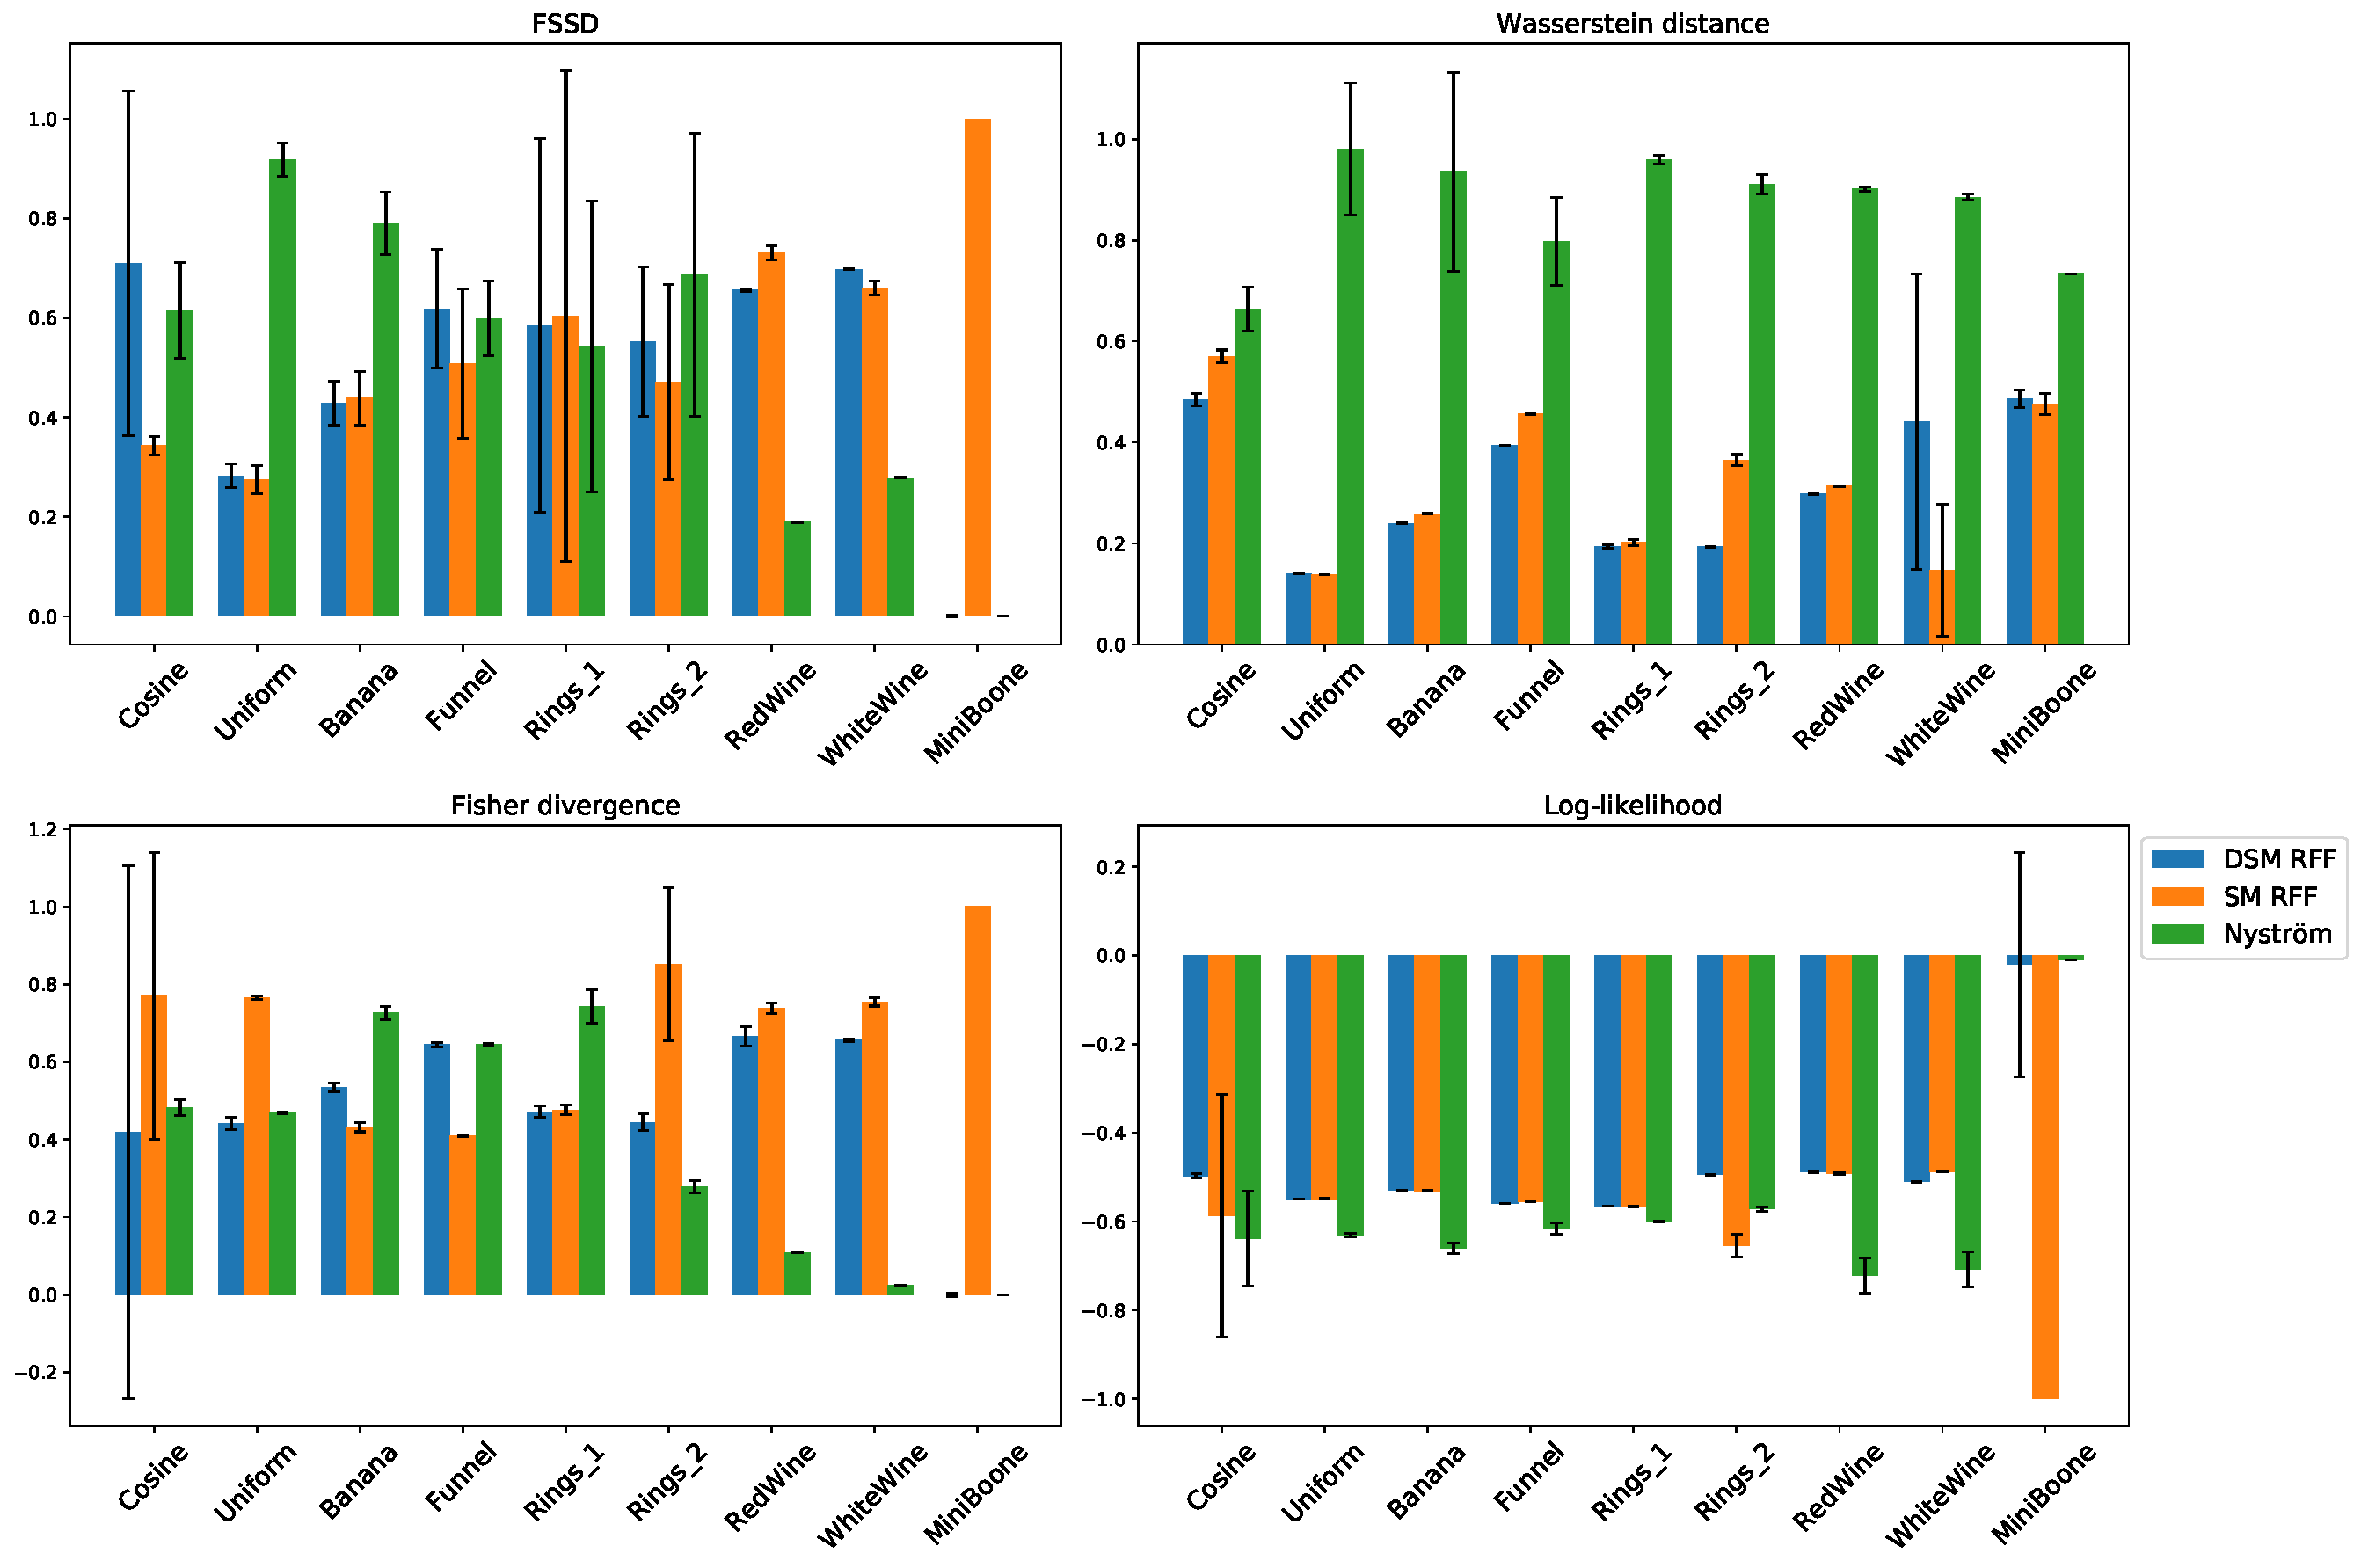
\includegraphics[width=\textwidth]{figures/score_matching/exps/metrics.pdf}
  \caption{Metrics on different datasets for different methods.
           For each dataset each metric was normalized across methods
           to have unit norm.
           We did it only for better visualization.}
  \label{fig:metrics}
\end{figure}

\begin{table}
\centering
\caption{Metrics for the data sets from UCI repository.}
\label{tab:metrics}
  \footnotesize
  \begin{tabular}{llrrrrr}
    \toprule
    Data set & Model & Log-likelihood & FSSD &
    \shortstack{Wasserstein \\ distance} & time, s \\
    \midrule
    RedWine & DSM RFF     & -11.64 & 0.38 & 0.24 & 62 \\
            & SM RFF      & -11.72 & 0.43 & 0.25 & 61 \\
            & Nystr\"om   & -17.23 & 0.11 & 0.73 & $0.2 \times 10^4$ \\
    WhiteWine & DSM RFF   & -12.81 & 0.57 & 0.33 & 180 \\
              & SM RFF    & -12.22 & 0.53 & 0.11 & 180 \\
              & Nystr\"om & -17.79 & 0.23 & 0.67 & $1 \times 10^4$ \\
    MiniBoone & DSM RFF   & -93.11 & 307.67 & 0.49 & $0.5 \times 10^4$ \\
              & SM RFF    & -4580.20 & $2 \times 10^8$ & 0.48 & $0.5 \times 10^4$ \\
              & Nystr\"om & -46.06 & 0.02 &  0.75 & $0.6 \times 10^4$ \\
    \bottomrule
  \end{tabular}
\end{table}







\section{Simultaneous Localization and Mapping with Random Features}
\label{sec:SLAM}

Since the last century, probabilistic state estimation has been a core topic in mobile robotics, often as part of the problem of simultaneous localization and mapping \cite{bailey2006simultaneous,durrant2006simultaneous}.
Recovery of a robot's position and a map of its environment from sensor data is a complicated problem due to both map and trajectory are unknown as well as the correspondences between observations and landmarks \cite{probabilistic}.

Well-known approaches to this problem, such as square root smoothing and mapping (SAM)\cite{SAM},
relied on regression-based techniques that leverage the problem's sparse structure to calculate a solution effectively.
However, this technique had a great disadvantage, i.e., we may need to collect all the data before trajectory estimation (batch updates)\cite{FASTisam}.
This method was improved in \cite{isam}, where incremental smoothing and mapping  (iSAM) was introduced.
iSAM requires expensive periodic batch steps to keep re-linearization and sparsity.
This method has been further improved in iSAM 2.0 \cite{isam2}. In iSAM 2.0 an effective graph structure,
the Bayes tree \cite{bayes}, is used to accomplish incremental variable reordering and just-in-time reordering,
thus reducing the bottleneck caused by batch variable reordering and re-linearization.
This method is widely used as state-of-the-art, and this work has gained several sequels, such as \cite{1sam, 2sam,3sam,4sam}.

Most trajectory estimation and mapping methods, including SAM-based ones, have considered the problem in a
discrete-time fashion.
However, discrete-time representations are constrained because they are not easily adapted to irregularly distributed poses or asynchronous measurements over trajectories.
Such limitations would be well addressed by a continuous-time version of the SAM problem where measurements regulate the trajectory at any time step.
The robot trajectory, seen from this perspective, is a function $\bm{x}(t)$,
which corresponds to a robot state at every time $t$. Simultaneous trajectory estimation and mapping (STEAM) presents the problem of estimating this function along with landmark positions \cite{barfoot,barfoot2017}.
In the work \cite{furgal} they formally derive a
continuous-time SLAM problem and demonstrates the use of a parametric solution for atypical SLAM
calibration problems.
The use of cubic splines to parameterize the robot trajectory can also be seen in the estimation schemes
in~\cite{br, fleps, droeschel2018efficient}.
In the work \cite{tong2013gaussian} the  parametric
state  representation  was proposed due  to
practicality and effectiveness.
% Based on the previous works, \cite{barfoot}
% suggested a GP model based on a
% regression approach to STEAM problem-solving.
The advantages of this method are that they can
precisely model  and  interpolate  asynchronous
data to  recover  a  trajectory  and  estimate
landmark positions.
The disadvantages of that algorithm are that it
requires batch updates and considerable
computational  problems that are natural for
regression.


In  the  work \cite{best}, the  critical  update  to
increase the efficiency of  existing  GP approach to
solve the  STEAM  problem was introduced.
It combines benefits of iSAM  2.0 and Barfoot's work \cite{barfoot2014batch}
and provide the GP-based  solution  to the  STEAM
problem  that  computationally  efficiently even for
large datasets.
However, in this work GP have several constraints to
be able to deal with sparse measurements and provide
robot position at any point of interest.

The main drawback of the paper is that the proposed GP
prior impose constraints on the kernel function and
thus limits the number of possible functions that GP
can model.
They use state-space formulation to conduct
computationally efficient inference for GP.
However, the efficiency is achieved by the means of
using kernel functions that impose Markovian structure on the trajectory:
it is supposed that two points on the trajectory are conditionally
independent given all other points if these two points are not neighboring.
However, in some cases the accuracy of the trajectory
estimate can be increased by adjusting the estimate
at the current point using all previous points in the trajectory, especially when the observations
contain a considerable amount of noise.

In recent years a lot of effort has been put to develop large-scale GP models without any constraints on the kernel function~\cite{rudi2017falkon, wang2019exact, munkhoeva2018quadrature}.
There are two main approaches to scale up the GP model.
The first one is based on Nystr{\"o}m approximation \cite{quinonero2005unifying}.
The idea is to approximate the kernel function using a finite set of basis functions that are based on eigenvectors of the kernel matrix.
This approach is data-dependent and needs updating the basis function when new observations arrive.
Another set of methods is based on Random Fourier Features \cite{rahimi2008random}.
In these approaches the basis functions (features) are constructed based solely on the kernel function and independent of the data set.
It provides additional computational benefits and is more attractive for SLAM problems.

In this section we develop random features based SLAM
approach.
It is constructed solely based solely on the kernel function
and independent of the data set.
It provides additional computational benefits compared to other approaches
and, therefore, is more attractive for SLAM problems.
We build a low-rank approximation of the kernel matrix.
It is dense, so we do not assume the conditional independence of the points on the trajectory.
At the same time we maintain reasonable computational complexity by limiting the number of random features.
We conduct several experiments and discuss the results of running the method on synthetic data and well-known real-world benchmarks.


\subsection{SLAM}
From a probabilistic point of view, there are two main forms of the problem: online-SLAM and FULL-SLAM. Online SLAM (\ref{online}) involves estimating the posterior over the current pose along the map:
\begin{equation} \label{online}
p\left(\bm{x}_{t}, \bm{l} | \mathbf{z}, \mathbf{u}\right),
\end{equation}
where $\bm{x}_{t}$ is the pose at time $t, \bm{l}$ is the map (in this work, we consider $\bm{l}$ to be the map of landmarks), and $\mathbf{z} = \begin{bmatrix}\bm{z}_(t_1) & \cdots \bm{z}(t_N)\end{bmatrix}$ and $\mathbf{u} = \begin{bmatrix}\bm{u}_(t_1) & \cdots \bm{u}(t_N)\end{bmatrix}$ are the measurements and controls, respectively.
In full SLAM (\ref{full}), we seek to calculate a posterior over the entire path $\mathbf{x} = \begin{bmatrix}\bm{x}_(t_0) & \cdots \bm{x}(t_N)\end{bmatrix}$ along with the map, instead of just the current pose $\bm{x}_{t}$:
\begin{equation}\label{full}
    \quad p\left(\mathbf{x}, \bm{l} | \mathbf{z}, \mathbf{u}\right).
\end{equation}

\subsection{RFF-SLAM}

We use GP regression with RFF to estimate the state variables corresponding to trajectory and map (landmarks).
Our model is as follows
\begin{equation}
\label{eq:gp_slam_model}
    \begin{aligned}
        \bm{x}(t) &\sim \mathcal{GP}(\bm{\mu}_x(t), \bm{k}(t, t')), \\
        \bm{l} &\sim \mathcal{N}(\bm{\mu}_l, \mathbf{L}), \\
        \bm{z}_i &= \bm{h}\left (
        \begin{bmatrix}
            {\bm x}(t_i) \\
            {\bm l}
        \end{bmatrix}
        \right ) + \bm{n}_i,
    \end{aligned}
\end{equation}
where ${\bm x}(t)$ is a state of the robot at timestamp $t$,
${\bm l}$ is a vector of $M$ landmarks,
$\bm{h}(\cdot)$ is a non-linear measurement model,
$\bm{n}_i \sim \mathcal{N}(\bm{0}, \mathbf{R}_i)$ is measurement noise,
$t_1, \ldots, t_N$ is a sequence of measurement times and
$(\bm{\mu}_l, \mathbf{L})$ are prior mean and the covariance of the landmarks positions.

The paper \cite{tong2013gaussian} uses GP for SLAM and provides the main equations to solve the problem.
We follow their approach with the difference that we utilize RFF approximation
(see Section~\ref{sec:random_fourier_features}) of the RBF kernel given by
\[
k(t, t') = \sigma^2 \exp \left ( -\frac{\|t - t'\|_2^2}{2 \sigma_l^2} \right ).
\]
For the RBF kernel its Fourier transform is defined by $p(\bm{w})$ being a Gaussian distribution $\mathcal{N}\left (0, \frac{1}{\sigma_l^2}\mathbf{I} \right )$.
Explicit mapping \eqref{eq:inner} allows working in
weight-space view
\[
{\bm x}(t) = {\bm \mu}_x(t) + \begin{bmatrix}
        \phi_1(t) {\bm b}_x^{(1)} \\
        \cdots \\
        \phi_d(t) {\bm b}_x^{(d)} \\
    \end{bmatrix}
    + \varepsilon,
    \quad {\bm b}_x^{(i)} \sim \mathcal{N}({\bm \mu}_b^{(i)}, \mathbf{K}_i), i = \overline{1, d},
\]
where $d$ is a state size,
${\bm b}_x^{(i)} \in \mathbb{R}^d$,
$\phi_i({\bm x})$ is a feature map for the $i$-th state variable
and $\mathbf{K}_i$ is a prior covariance matrix of the random variable
${\bm b}_x^{(i)}$.
In principle, the same feature map can be used for all variables,
however, it can be reasonable to use different features
(corresponding to different kernels) to model different types of variables
(for example, coordinates on the map and angles).

Let us denote
\begin{gather}
    {\bm b} = \begin{bmatrix}
        {\bm b}_x^{(1)} \\
        \cdots \\
        {\bm b}_x^{(d)} \\
        {\bm l}
    \end{bmatrix},
    {\bm \mu} = \begin{bmatrix}
        {\bm \mu}_b^{(1)} \\
        \cdots \\
        {\bm \mu}_b^{(d)} \\
        {\bm \mu}_l
    \end{bmatrix},
    \mathbf{K} = \begin{bmatrix}
        \mathbf{K}_1 & & \\
        & \ddots & \\
        & & \mathbf{K}_d
    \end{bmatrix},
    \nonumber \\
    \mathbf{P} = \begin{bmatrix}
        \mathbf{K} & \\
        & \mathbf{L} \\
    \end{bmatrix},
    {\bm \Phi}_i = \begin{bmatrix}
        \phi_1(t_i) & & & \\
        & \cdots & & \\
        & & \phi_d(t_i) & \\
        & & & \mathbf{I}_{2M}
    \end{bmatrix},
    \label{eq:system_variables} \\
    \mathbf{R} = \begin{bmatrix}
        \mathbf{R}_1 & & \\
        & \ddots & \\
        & & \mathbf{R}_N
    \end{bmatrix}. \nonumber
\end{gather}
Now to obtain both the robot states and landmarks position
${\bm b}$ we employ maximum a posteriori (MAP) estimate
\begin{align}
\label{eq:map_equation}
    p({\bm b} | {\bm z}) &=
    \frac{p({\bm z} | {\bm b}) p({\bm b})}{p({\bm z})} \nonumber \\
    &\propto
    -\frac12 \left (
        \sum_{i=1}^N
        \|{\bm z_i} - {\bm h}({\bm \Phi}_i {\bm b})\|_{\mathbf{R}_i}^2
        + \|{\bm b} - {\bm \mu}\|_{\mathbf{P}}^2
    \right ) \nonumber \\
    & \rightarrow \max_{{\bm b}}.
\end{align}
To solve the problem we do the following.
Suppose, that we have an initial guess $\bar{\bm{b}}$.
We update the estimate iteratively by finding the optimal perturbation vector $\delta \bm{b}^*$ for the linearized measurement model.
Namely, we apply the first order Taylor expansion to the measurements model
\[
    \bm{h}({\bm \Phi}_i {\bm b}) \approx \bm{h}({\bm \Phi}_i \bar{\bm{b}}) + \mathbf{H}_i \delta \bm{b}, \quad
    \mathbf{H}_i = \left . \frac{\partial \bm{h}({\bm y}}{\partial \bm{y}} \right |_{{\bm y} = {\bm \Phi}_i \bar{\bm{b}}}.
\]
Plugging linearized measurement into \eqref{eq:map_equation}
we obtain the following optimization problem
\begin{align*}
    \delta \bm{b}^* = \argmin_{\delta \bm{b}}
    \frac12 \left ( \sum_{i = 1}^N
    \|\bm{z}_i - \bm{h}({\bm \Phi}\bar{\bm{b}}) -
    \mathbf{H}_i{\bm \Phi}_i\delta \bm{b}\|_{\mathbf{R}_i}^2 +
    \|\bar{\bm{b}} + \delta \bm{b} - \bm{\mu}\|_{\mathbf{P}}^2
    \right ).
\end{align*}
The solution is given by
\begin{gather}
    \delta {\bm b}^* = \mathbf{A}^{-1}{\bm g},
    \nonumber \\
    \mathbf{A} = \sum\limits_{i=1}^N
        {\bm \Phi}_i^\top \mathbf{H}_i^\top \mathbf{R}_i^{-1} \mathbf{H}_i {\bm \Phi}_i
        + \mathbf{P}^{-1},
    \label{eq:state_update}
    \\
    {\bm g} = \sum\limits_{i=1}^N
        {\bm \Phi}_i^\top \mathbf{H}_i^\top \mathbf{R}_i^{-1} \left (
    {\bm z}_i - {\bm h}(\Phi_i \bar{{\bm b}})
    \right ) + \mathbf{P}^{-1} \left (
    \bar{{\bm b}} - {\bm \mu}_b
    \right ). \nonumber
\end{gather}

We update the model parameters
$\bar{{\bm b}} \gets \bar{{\bm b}} + \delta {\bm b}^*$,
then update all the matrices and vectors in \eqref{eq:system_variables}
and repeat the procedure predefined number of iterations or until convergence.
The described approach is known as Gauss-Newton method to solve
non-linear least squares problems, and it is used in
\cite{tong2013gaussian, barfoot}.
It does not guarantee convergence, so in this work
we apply Levenberg-Marquardt approach.
It modifies the system
\begin{equation}
\label{eq:levenberg_marquardt}
    \delta {\bm b}^* = \left (
        \mathbf{A} + \lambda {\rm diag} \left ( \mathbf{A} \right )
    \right )^{-1} {\bm g}
\end{equation}
where $\lambda$ is a dampening parameter.
The overall update procedure is summarized in Algorithm~\ref{alg:state_update}.

The size of the system matrix $\mathbf{A}$ is
$(Dd + 2M) \times (Dd + 2M)$ for two-dimensional landmarks.
The top-left block of size $Dd \times Dd $ of the matrix corresponds
to the weights ${\bm b}$ and is typically dense.
The bottom-right block of size $2M \times 2M$ corresponds
to landmarks and it is usually diagonal
(because we assume that landmarks are independent).
Therefore, the cost of solving \eqref{eq:state_update}
is $\mathcal{O}(D^3d^3 + MDd)$ using Schur complement.
However, we use iterative solver and in practice it converges
much faster.
The cost of construction of the matrices in \eqref{eq:state_update}
is $\mathcal{O}(N(D^2d^2 + M)$.
The total complexity is
$\mathcal{O}(\max (ND^2d^2 + NM), (D^3d^3 + MDd))$.

When we use the iterative solver that utilizes only matrix-vector
products, we can also rearrange operations to obtain different
computational complexity.
Instead of calculating the matrix $\mathbf{A}$ explicitly
we can multiply each term of the sum in \eqref{eq:state_update}
by a vector and then take the sum.
Taking into account that matrices $\mathbf{R}_i$ are (usually)
diagonal, the part of the Jacobi matrix $\mathbf{H}_i$ that
corresponds to derivatives of w.r.t landmarks is block-diagonal,
the complexity of matrix-vector product for one term in the sum
is $\mathcal{O}((M + D)d)$.
The overall complexity of solving the system is
$\mathcal{O}(N(M + D)d k)$, where $k$ is the number of iterations.


\subsubsection{State prior}
In GP regression it is common make zero-mean assumption,
i.e. ${\bm \mu}(t) = {\bm 0}$.
However, having good prior ${\bm \mu}(t)$ is essential
when modeling trajectory with GP, because usually
shift-invariant kernel functions are used.
Therefore, GP with such kernels is most suited to model
stationary functions.
This does not always apply to trajectories.
Non-stationarity can be accounted by non-zero mean function
${\bm \mu}(t)$.
Here we use one of two prior mean functions.
\begin{enumerate}
    \item Motion model
    \[
        \bm{\mu}_x(t_i) = \mathbf{F}(t_i) \hat{\bm{x}}(t_{i - 1}) + \mathbf{B}(t_i) \bm{u}(t_i),
    \]
    where $\mathbf{F}(t), \mathbf{B}(t)$ are time-dependent
    system matrices.
    We use this model if we have odometry measurements.
    \item Smoothing splines applied to the estimated
    trajectory with smoothing parameter $0.98$
    (we used De Boor's formulation,
    see~\cite{bde2001practical}).
    We also use weights that are inverse proportional to the
    data fit error $\|{\bm z}_i - {\bm h}({\bm \Phi}_i {\bm b})\|_{\mathbf{R}_i}$.
    The motivation behind this prior mean model is the following:
    in case of some non-stationarity the GP can produce inaccurate predictions
    (for example, there can be oscillations in regions where the function quickly changes its value).
    Smoothing the trajectory reduces such effects.
\end{enumerate}
With a non-zero prior mean for the trajectory we can set
all mean vectors ${\bm \mu}_b^{(i)}$ to zero,
thus, the GP will only correct the errors of the mean
${\bm \mu}(t)$.
The whole trajectory estimate is updated with every new measurement,
so we also update the prior
$\bm{\mu}_x(t_i)$ for all $i=1, \ldots, N$
for each new observation.


\begin{algorithm}
\caption{Update state at measurement times}
\label{alg:state_update}
    \begin{algorithmic}[1]
        \State Initial values $\bar{\bm{b}}$, measurement times $t_1, \ldots, t_N$, measurements $\mathbf{z}$, $\varepsilon$, maximum number of iterations $K$
        \State $n \gets 0$
        \Repeat
            \State Using $\bar{\bm{b}}$ update vectors and matrices in \eqref{eq:system_variables}
            \State Calculate update $\delta \bm{b}^*$ by
            applying \eqref{eq:levenberg_marquardt} to solve \eqref{eq:state_update}
            \State $\bar{\bm{b}} \gets \bar{\bm{b}} + \delta \bm{b}^*$
            \State $n \gets n + 1$
        \Until relative error is less than $\varepsilon$ \textbf{or} $n = K$
    \end{algorithmic}
\end{algorithm}

\subsection{Experiments}
In this section, we evaluate our approach
on several synthetic 2D trajectories
as well as real-world benchmarks.
In all our experiments, we consider the state vector to be a 2D pose:
\[
    \bm{x}(t) = \begin{bmatrix}
    x(t) \\
    y(t) \\
    \alpha(t)
    \end{bmatrix}.
\]
We use the range/bearing observation model which takes the form
\begin{equation}
\label{eq:observation_function}
    \bm{h}\left (\begin{bmatrix}
            \bm{x}(t_i) \\
            \bm{l}_j
        \end{bmatrix}
    \right ) =
    \begin{bmatrix}
        \sqrt{(x_j - x(t_i))^2 + (y_j - y(t_i)^2} \\
        {\rm atan2}(y_j - y(t_i), x_j - x(t_i)) - \alpha(t_i)\\
    \end{bmatrix} ,
\end{equation}
where $\bm{l}_j = \begin{bmatrix}
x_j \\
y_j
\end{bmatrix}$ is a vector of coordinates of $j$-th landmark.
The covariance matrices $\mathbf{R}_j$ are
given and typically determined by the precision of the sensor.
In some of the experiments we consider
only range measurements
(the first row in measurement model),
in some of the experiments we have only
bearing measurements (the second row in the measurement model)
and in other experiments we have both
range and bearing measurements.
The proposed approach is compared against model based
on linear time-variant stochastic differential equation (LTV SDE)
\cite{barfoot}\footnote{The implementation was taken from
\url{https://github.com/gtrll/gpslam}}.


To evaluate the quality of the estimated trajectories, we calculate
two metrics.
\begin{itemize}
    \item Absolute Pose Error (APE).
    This metric estimates global consistency of the trajectory.
    It is based on the relative pose on the estimated trajectory and ground truth trajectory:
    \[
        e_i^{abs} = \widehat{\mathbf{P}}_i \ominus \mathbf{P}_i =
        \left ( \mathbf{P}_i \right )^{-1} \widehat{\mathbf{P}}_i,
        \quad
        \mathbf{P}_i, \widehat{\mathbf{P}}_i \in SE(3),
    \]
    where $\mathbf{P}_i, \widehat{\mathbf{P}}_i$ are ground truth pose and estimated
    pose at time step $t_i$ represented by an element from $SE(3)$ group of rigid body transformations (translation and rotation).
    We represent 2D points as 3D point by adding zero $z$-coordinate and zero roll and pitch
    angles.
    Then we can calculate the translational error
    \[
        {\rm APE}_{trans} = \sqrt{\frac{1}{N} \|trans(e_i^{abs})\|_2^2},
    \]
    where $trans(e)$ is a translational part of $e$.
    And we can calculate the rotational error
    \[
        {\rm APE}_{rot} = \sqrt{\frac{1}{N} \|rot(e_i^{abs})\|_2^2},
    \]
    where $rot(e)$ is a rotational part of $e$.

    \item Relative Pose Error (RPE).
    This metric estimates the local consistency of the trajectory.
    It is invariant to drifts, i.e., if we translate and rotate the whole trajectory
    the RPE error will remain the same.
    RPE is based on the relative difference of the poses on the estimated trajectory and
    ground truth trajectory:
    \begin{align*}
        e_i^{rel} = \hat{\delta}_i \ominus \delta_i =
        \left (
            \left ( \mathbf{P}_{i - 1} \right )^{-1} \mathbf{P}_i
        \right )^{-1}
        \left (
            \left ( \widehat{\mathbf{P}}_{i - 1} \right )^{-1} \widehat{\mathbf{P}}_i
        \right )
        \\
        \mathbf{P}_i, \widehat{\mathbf{P}}_i \in SE(3),
    \end{align*}
    where $\mathbf{P}_i, \widehat{\mathbf{P}}_i$ are as in APE.
    Similarly to APE, we calculate translational and rotational errors
    \[
        {\rm RPE}_{trans} = \sqrt{\frac{1}{N} \|trans(e_i^{rel})\|_2^2},
    \]
    \[
        {\rm RPE}_{rot} = \sqrt{\frac{1}{N} \|rot(e_i^{rel})\|_2^2}.
    \]
\end{itemize}


\subsubsection{Synthetic trajectories}
We generated $10$ different random trajectories, for each trajectory we conducted several experiments
with different noise level in observations,
different number of landmarks (from $5$ to $100$)
and different measurement types (range, bearing, range/bearing).
The noise was generated from Gaussian distribution with standard
deviation varying in $[1, 5]$ interval for range measurements
and bearing varying in $[1^\circ, 10^\circ]$ interval.

\paragraph*{Number of features $D$}
For the synthetic dataset we conducted experiments with different number of features.
We observed that for a small number of features ($D \sim 10$) the trajectory starts diverging when its length increases (at about $100$ observations).
Increasing the number of features increases the length of the trajectory for which the estimate does not diverge.
For the trajectories that we used in our experiments $D=100$ was
enough to obtain good state estimates.

\paragraph*{Kernel parameters.}
The main kernel parameter is its lengthscale $\sigma_l$.
Typically, in the GP regression model the lengthscale is one of the most important parameters affecting the quality of the model.
It controls the smoothness of the obtained approximation.
Larger lengthscale should be used for smooth trajectories and smaller values for
less smooth trajectories.

In our experiments a rather wide kernel worked well,
we set $\sigma_l = 3.0$.
%An example of the estimated trajectories is given in Figure~\ref{fig:rand_2d}.
% In case of range only measurements there is no
% information about the heading of the robot
% in observation, so our approach cannot estimate it (it returns constant value).
% In this case we calculate the bearing as an angle of the movement direction.
The qualitative results can be found in Table~\ref{tab:rand_2d_errors}.
We can see that in the case of range and range-bearing measurements
the proposed approach looks more accurate.

We also study the dependency of the estimation error on the noise level
and the number of landmarks.
In Figure~\ref{fig:synthetic_noise_distr}
you can see the APE translation errors
for different noise levels, the number of landmarks and measurement types.
We make several observations based on these results.
\begin{itemize}
    \item Our approach does not estimate bearing in the range-only measurements because there is no information about bearing in the data.
    In this case we calculate heading by
    calculating the movement direction of the estimated trajectory.
    Barfoot's method handle this situation due to their mean prior based on
    the differential equation.

    \item The proposed approach provides better rotation errors in all cases.

    \item The translation errors in range only
    setting and rotation errors of RFF
    approach in bearing only measurements
    increase slower with noise level compared
    to LTV SDE errors.
    For range-bearing case the difference is less significant.
\end{itemize}

\begin{figure}
    \centering
    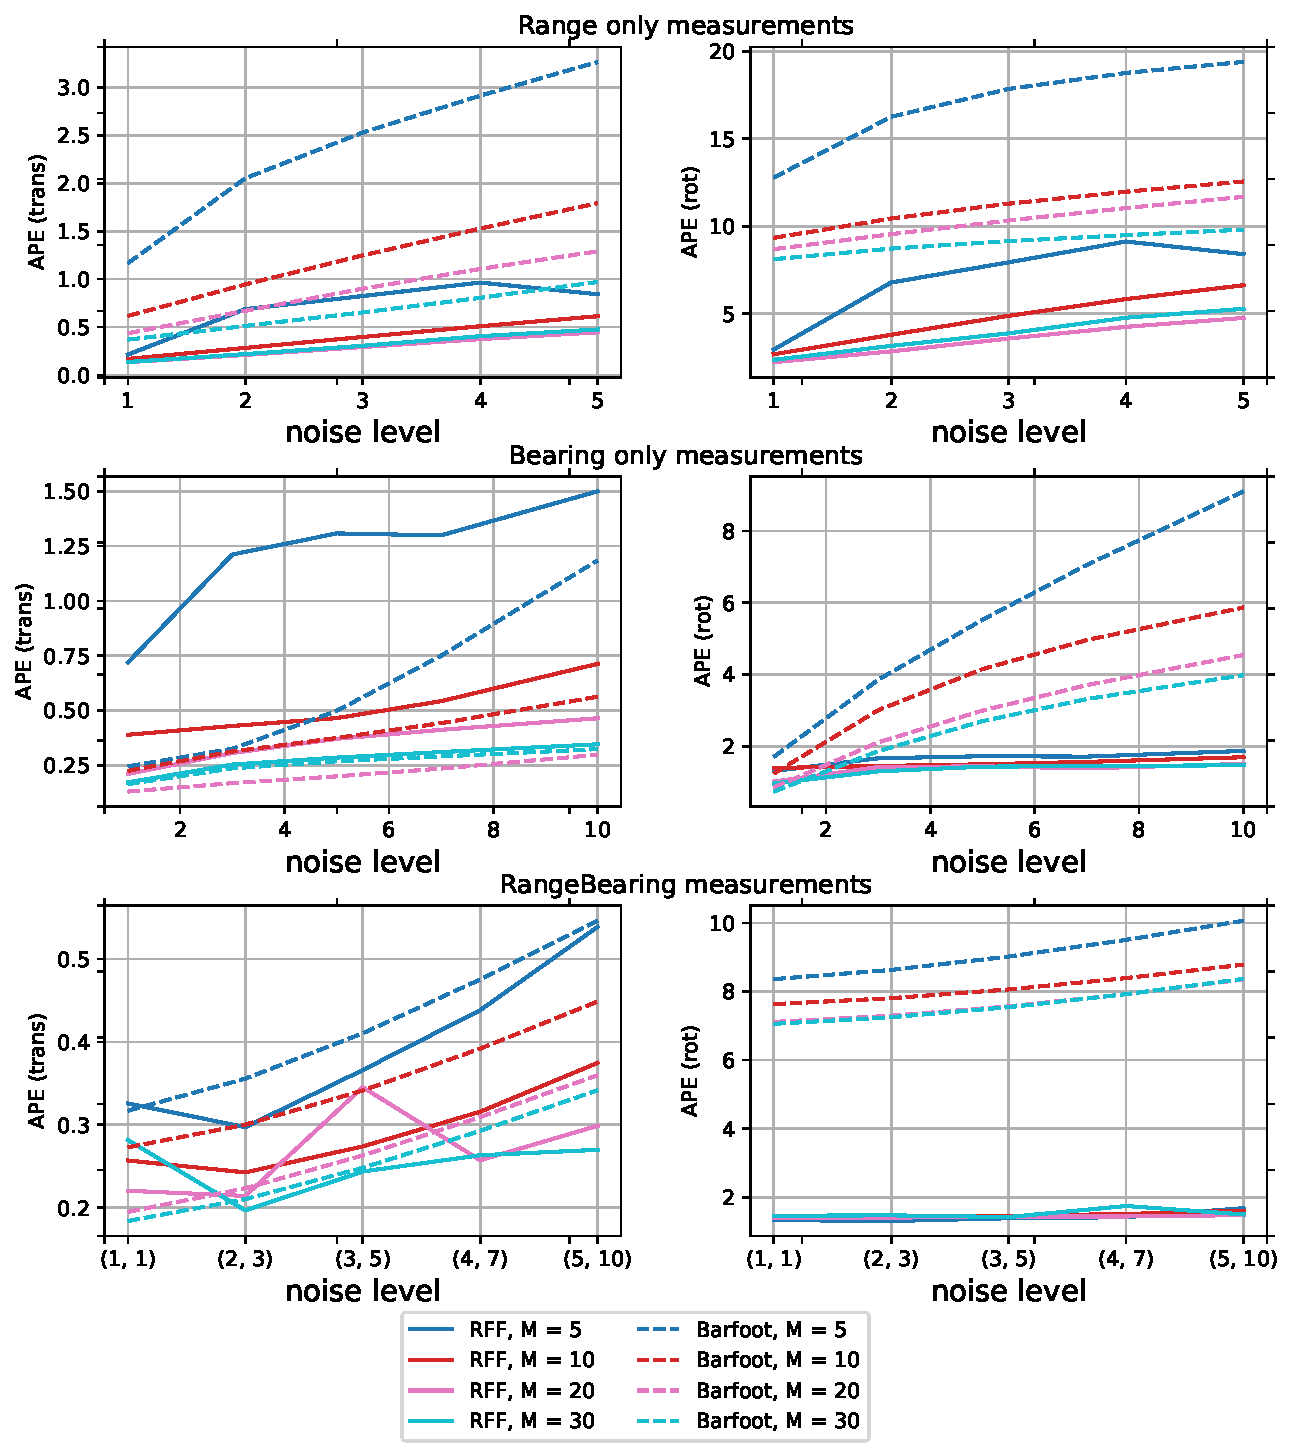
\includegraphics[width=0.8\textwidth]{figures/slam/synthetic_noise_distr.pdf}
    \caption{Average APE errors for synthetic trajectories at different noise levels
    and number of landmarks}
    \label{fig:synthetic_noise_distr}
\end{figure}

\begin{table}[]
    \centering
    \caption{Relative Errors for synthetic trajectories}
    \label{tab:rand_2d_errors}
    \begin{tabular}{cc|c c c}
     & & Pos. & Rot. & Landmarks \\
     \toprule
     RangeBearing & RFF & 0.022 & \textbf{0.154} & 6e-4 \\
     & LTV SDE & 0.025 & 5.602 & 0.110 \\
     \hline
     Range & RFF & \textbf{0.016} & \textbf{0.320} & 1e-6 \\
     & LTV SDE & 0.025 & 5.580 & 0.003 \\
     \hline
     Bearing & RFF & 0.035 & \textbf{0.152} & 8e-6 \\
     & LTV SDE & \textbf{0.025} & 1.200 & 0.016 \\
     \bottomrule
    \end{tabular}
\end{table}


\subsubsection{Autonomous Lawn-Mower}
In this experiment we evaluate our approach on a Plaza data set
collected from an autonomous
lawn-mower~\cite{djugash2010geolocation}.
The data set contains range measurements recorded using
time-of-flight and odometry measurements.
Odometry measurements come more frequently than range measurements.
The ground truth data was collected from GPS measurements
and according to \cite{djugash2010geolocation} its accuracy
is $2$cm.

The resulting trajectory is given in
Figure~\ref{fig:autnomous_lawn_mower}.
In this experiment we did batch updates, i.e.
we updated the trajectory after each new $5$ range measurements.
The motion model based prior was used as we have odometry
measurements.
We can see slight oscillations of the estimated trajectory.
They can be explained by the nature of the Fourier features.
However, the errors are comparable as can be seen from Table~\ref{tab:real_benchmarks_errors}.
The estimated trajectories are depicted in Figure~\ref{fig:autnomous_lawn_mower}.

\begin{figure}[h]
    \centering
    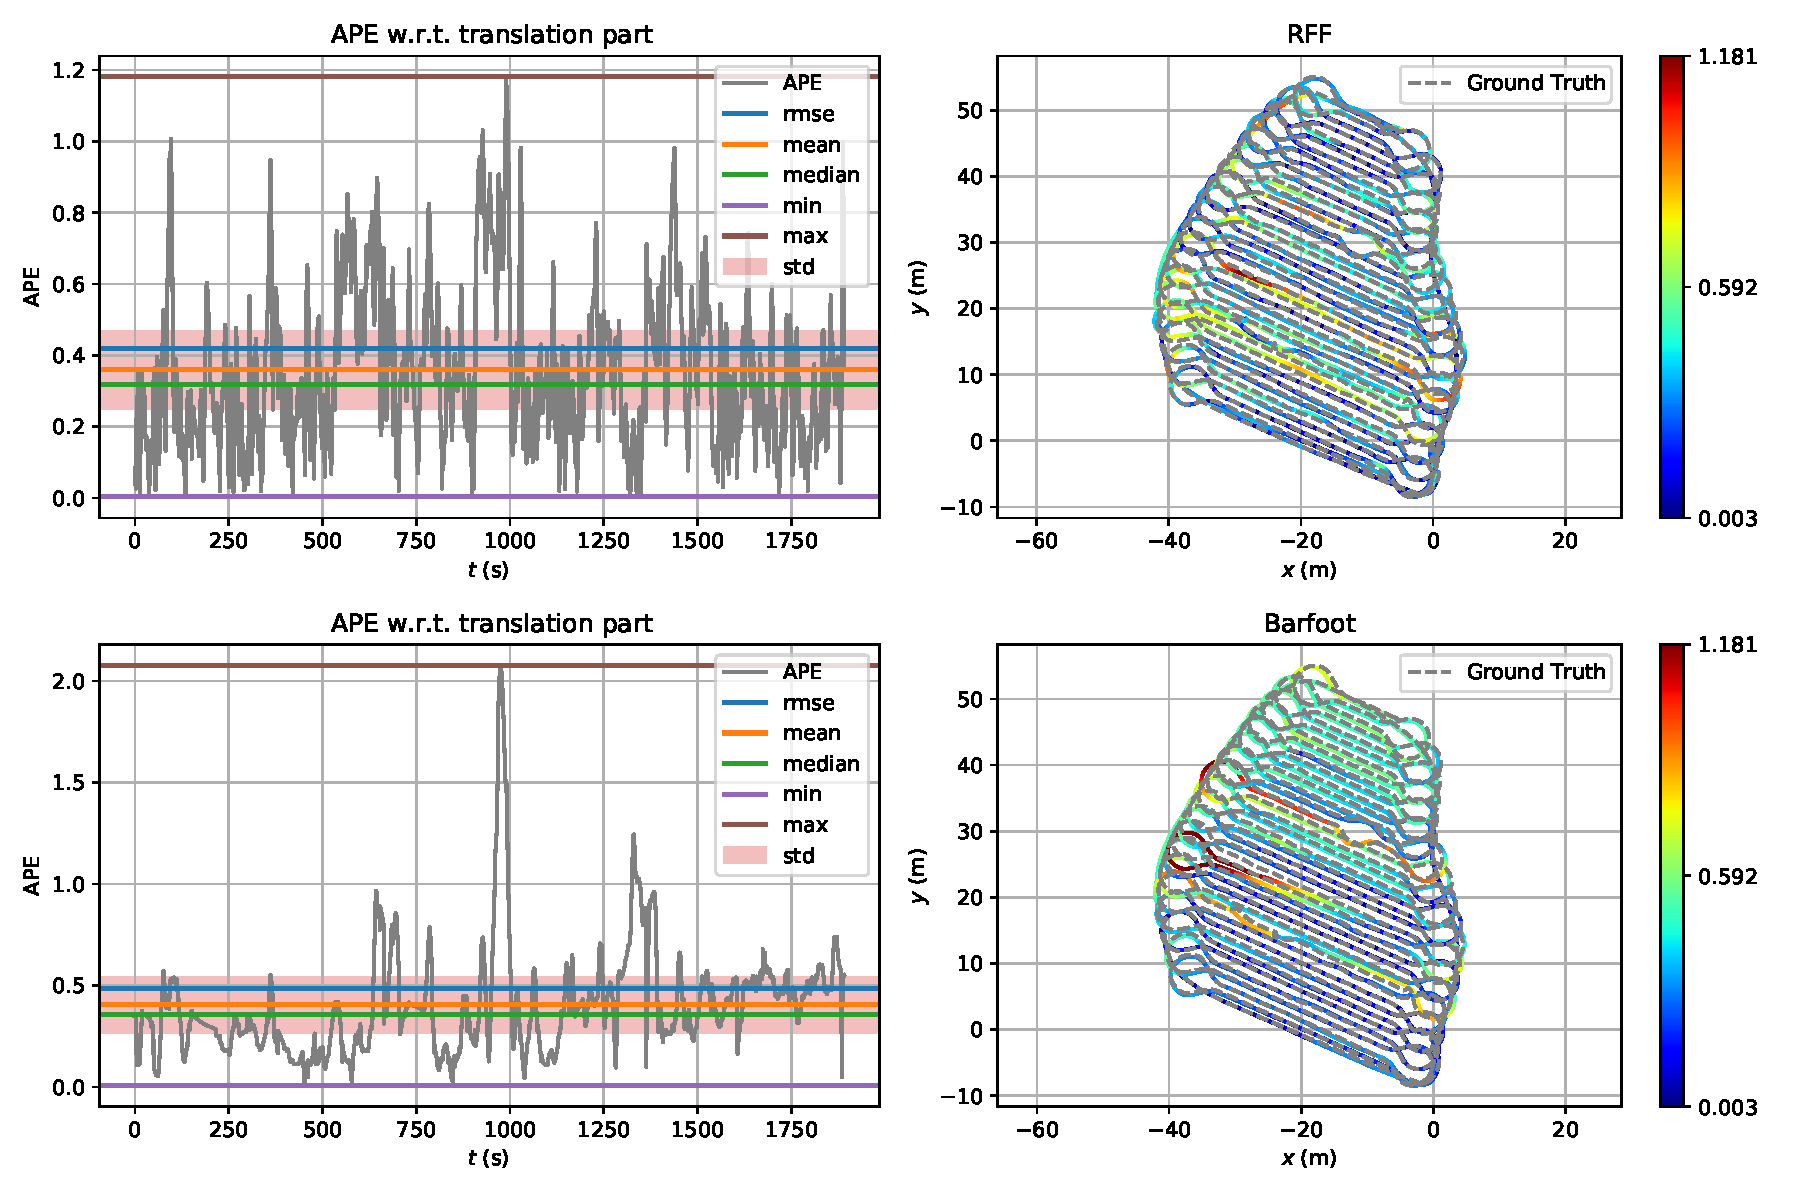
\includegraphics[width=0.8\textwidth]{figures/slam/plaza_ape.pdf}
    \caption{Distribution of APE errors along the trajecotry for Autonomous Lawn-Mower benchmark}
    \label{fig:autnomous_lawn_mower}
\end{figure}

\subsubsection{KITTI-projected dataset}

To evaluate our approach, we proceed with the world-famous dataset KITTI odometry\cite{kitti}.
We chose the dataset part that contains stereo sequences -- a sequence of stereo images taken while moving along a
specific trajectory.
The dataset includes stereo images, ground truth trajectory and camera information.
For our approach, we need a dataset in 2D with observations and bearing.
To extract observations in the form \eqref{eq:observation_function} we do visual SLAM from ORB-SLAM2 \cite{mur2017orb}.
For each keypoint we find its coordinates in the local frame\cite{multiview}.
Therefore, we can calculate bearing observations for each keypoint.
Thus, the keypoints in this case play the role of landmarks and we have bearing measurements.
The pipeline to project KITTI into a 2D dataset is following:

\begin{itemize}
\item Input: KITTI-odometry dataset (e.g. sequence 08);
\item Run ORB-SLAM2 to get observations (keypoints, timestamps);
\item Correct camera pose and keypoints by a transformation term that aligns with the vertical axis to make them independent of their original camera pose
\begin{equation}  \label{eq:corr}
R_t \cdot R_{correction} = \mathrm{Exp}([0,0,\alpha]^{\top});
\end{equation}
\item Calculate weights for each observations based on how much time this point was observed/visited;
\item Filter observations;
\item Do orthonormal projection for each observation;
\item Calculate bearing.
\end{itemize}

The number of landmarks (keypoints) is $80771$.
With such a big number of landmarks, the experiments are very slow, so we reduced the number of landmarks to $3975$.
We selected the landmarks randomly with probabilities proportional to their weights, but for each keyframe
we left not less than $10$ landmarks.
Also, to speed up the calculations we split the trajectory
into $10$ consecutive slices, do estimation on each slice
independently and then average the estimation errors.

The extracted data we then use in our approach to estimate the trajectory.
To check our assumption that kernels with dense precision
matrices should work better in case of noisy observations,
we also generated a noisy version of the KITTI-projected
dataset.
To do so, we added Gaussian noise with standard deviation $\sigma$.

The results are given in Table~\ref{tab:real_benchmarks_errors}.
We can see that without additional noise the results are comparable (with RFF based approach being slightly better).
When we increase the amount of noise, absolute errors of our approach remains the same
while errors for LTV SDE increase.

\begin{table}[ht]
    \centering
    \caption{Real-world benchmark errors.}
    \label{tab:real_benchmarks_errors}
    \begin{tabular}{c|c|c|c|c}
    \multicolumn{5}{l}{}\\[-0.5em]
    \multicolumn{5}{c}{Autonomous Lawn-Mower} \\
    \multicolumn{5}{l}{}\\[-0.7em]
    \toprule
    & APE (trans) & APE (rot) & RPE (trans) & RPE (rot) \\
    \hline
    LTV SDE & $0.48$ & $1.44$ & $0.021$ & $0.10$ \\
    RFF & $0.42$ & $2.25$ & $0.026$ & $0.54$ \\
    \bottomrule

    \multicolumn{5}{l}{}\\[-0.5em]
    \multicolumn{5}{c}{KITTI-projected} \\
    \multicolumn{5}{l}{}\\[-0.7em]
    \toprule
    LTV SDE & $5.130$ & $1.059$ & $0.068$ & $0.113$ \\
    RFF & $5.070$ & $0.489$ & $0.040$ & $0.048$ \\
    \bottomrule

    \multicolumn{5}{l}{}\\[-0.5em]
    \multicolumn{5}{c}{KITTI-projected + noise, $\sigma=1^\circ$} \\
    \multicolumn{5}{l}{}\\[-0.7em]
    \toprule
    LTV SDE & $5.126$ & $1.086$ & $0.068$ & $0.133$ \\
    RFF & $5.070$ & $0.544$ & $0.0454$ & $0.052$\\
    \bottomrule

    \multicolumn{5}{l}{}\\[-0.5em]
    \multicolumn{5}{c}{KITTI-projected + noise, $\sigma=3^\circ$} \\
    \multicolumn{5}{l}{}\\[-0.7em]
    \toprule
    LTV SDE & $5.491$ & $3.136$ & $0.139$ & $0.259$ \\
    RFF & $5.075$ & $1.027$ & $0.073$ & $0.115$ \\
    \bottomrule

    \multicolumn{5}{l}{}\\[-0.5em]
    \multicolumn{5}{c}{KITTI-projected + noise, $\sigma=5^\circ$} \\
    \multicolumn{5}{l}{}\\[-0.7em]
    \toprule
    LTV SDE & $12.915$ & $5.114$ & $0.242$ & $0.358$\\
    RFF & $5.077$ & $1.304$ & $0.084$ & $0.119$ \\
    \bottomrule
    \end{tabular}
\end{table}



\chapter{Conclusion}
\label{sec:conclusion}

This thesis contributes to the Gaussian Process models and kernel methods
as well as different machine learning techniques.

In Chapter~\ref{chap:gp_on_grids}, we considered regression problems
where the data set has either a full-factorial or an incomplete factorial
design of experiments.
Using the special structure of the data set, we developed
a computationally efficient technique for the exact inference of the GP model.
We also provided a special regularization for such cases
that allows the avoidance of the degeneration of the model and improves the overall quality.
The experimental section in this chapter demonstrates
the good performance of the approach and justifies low computational complexity.

Chapter~\ref{chap:unstructured_datasets} develops a general method
for an approximation of the kernel function based on randomized feature maps.
We propose a quadrature-based approach to building such feature maps
allowing us to obtain a low approximation error with a small number of features
and, thus, reduceing the computational complexity.
The theoretical analysis provides error bounds for the developed technique.
The experiments confirm the superiority of the method compared to other
random features-based approaches.

Chapter~\ref{chap:applications} is dedicated to applications of the developed methods.
We consider three different problems: tensor completion, probability density estimate
and simultaneous localization and mapping.
For the tensor completion problem, we developed an initialization scheme based on the
GP model.
We suppose that the function that generates tensor values is smooth and
model it by combining the GP model with a tensor-train based approximation method.
As a result, we developed a general tensor completion approach.
The experiments proved that the proposed initialization improves the overall quality.

We also applied the random features approach to the density estimate problem.
In this case we derived an analytical solution for the denoising score matching loss
which was impossible to derive using the exact GP model or Nystr{\"o}m-type approximations.
The resulting model has natural additional regularization.
The performance is also improved compared to the Nystr{\"o}m-based models.

Finally, the developed large-scale GP models allowed to re-utilize it
in simultaneous localization and mapping problems.
In robotics, they use state-space formulation of the GP model and a restricted
class of kernel functions that give a high computational performance.
With the proposed approach, we keep low computational complexity
but also enjoy the advantages of a broader class of kernel that we can apply.
We demonstrate that it can improve the quality of the estimates in some cases,
especially when there is a considerable amount of noise in observations.






Currently, deep neural networks outperform other techniques in many
problems.
Interestengly, there is a connection between neural networks
and kernel methods.
One of the first work in this direction is \citep{williams1996computing} which
showed that single-layer network with infinite number of neurons is equivalent
to Gaussian Process.
More modern works \citep{lee2017deep,jacot2018neural} show the connection
between deeper neural networks with Gaussian Processes and kernels.
The work \citep{daniely2017sgd} studies the behaviour of the
neural network with all the weight random except the last one which
is learnt using SGD.
This can be seen as random feature model.

In light of the mentioned works it is interesting to study how the properties
of random feature models (and kernels) can be transferred
to deep neural networks in practice.
For example, double descent phenomenon is encountered in over-parameterized
neural networks.
However, in some architectures it is impossible to observe it \citep{ba2019generalization},
while in random feature models it seems to be more robust \citep{mei2019generalization}.
So, the question is whether random features idea could help to develop
over-parameterized architectures with better double descent guarantees.

Also it is interesting to study whether random feature models can be helpful
in neural network compression.
In paper \citep{frankle2018lottery} the authors introduced Lottery Ticket Hypothesis
which states that a network contains smaller sub-network that can achieve
the same performance as the whole network when trained in isolation.
In context of the hypothesis shallow neural sub-networks are equivalent
to random feature models \citep{malach2020proving}.
So, further studying this connection and finding a way to apply
random features idea to compress neural network may be a promising
research direction.

Finally, I believe that in existing pipelines there are parts that
can be efficiently approximated using randomized maps.
For example, in recent work \citep{choromanski2020rethinking} they applied
random features approach to approximate attention mechanism.
Also, it can be fruitful to replace some traidtional layers or computations
by a more complicated kernel version and then reduce the complexity
using some kind of approximation.












%% ----------------------------------------------------------------
% Now begin the Appendices, including them as separate files

\addtocontents{toc}{\vspace{2em}} % Add a gap in the Contents, for aesthetics

\appendix % Cue to tell LaTeX that the following 'chapters' are Appendices

\chapter{Additional results for Quadrature-based features}

\section{Proof of Proposition 3.6}
\subsection{Variance of the degree $(3, 3)$ quadrature rule}
Let us denote $\mathbf{q} = \begin{pmatrix} \mathbf{x}\\ \mathbf{y} \end{pmatrix} \in \mathcal{X}^2$,
$k(\mathbf{q}) = k(\mathbf{x}, \mathbf{y})$,
$h_j(\mathbf{q}) = d \frac{f_{\mathbf{xy}}(-\rho_j \mathbf{Qv}_j) + f_{\mathbf{xy}}(\rho_j \mathbf{Qv}_j)}{2 \rho_j^2} - k(\mathbf{q}) =
s_j(\mathbf{q}) - k(\mathbf{q})$.
Then it is easy to see that $\mathbb{E}h_j(\mathbf{q}) = 0$.

Let us denote $I(\mathbf{q}) = SR^{3, 3}_{\mathbf{Q}_1,\rho_1}(f_{\mathbf{xy}})$,
$g(\mathbf{q}) = I(\mathbf{q}) - k(\mathbf{x}, \mathbf{y})$.
Using the above definitions we obtain
\begin{equation}
\begin{split}
\label{eq:variance_2_full}
\mathbb{V} g(\mathbf{q}) = \mathbb{V}\left ( 1 - \sum_{j = 1}^{d + 1}\frac{d}{(d + 1)\rho_j^2} \right) +
\mathbb{E} \left ( \frac{1}{d + 1} \sum_{i = 1}^{d + 1} h_i(\mathbf{q})\right)^2 \\
+ 2 cov \left ( 1 - \sum_{j = 1}^{d + 1}\frac{d}{(d + 1)\rho_j^2}, \frac{1}{d + 1} \sum_{i = 1}^{d + 1} h_i(\mathbf{q}) \right ).
\end{split}
\end{equation}
%%%%%%%%%%%%%%
Variance of the first term
\begin{align}
\label{eq:variance_2_first_term}
\mathbb{V}\left (1 - \sum_{j = 1}^{d + 1}\frac{d}{(d + 1)\rho_j^2} \right ) &= \mathbb{E}\left (1 - \sum_{j = 1}^{d + 1}\frac{d}{(d + 1)\rho_j^2} \right )^2 \nonumber\\&=
\mathbb{E} \left ( 1 - \sum_{j = 1}^{d + 1}\frac{2d}{(d + 1)\rho_j^2} + \left ( \sum_{j = 1}^{d + 1}\frac{d}{(d + 1)\rho_j^2} \right )^2\right) \nonumber \\
&=1 - 2 + \frac{d}{(d + 1)(d - 2)} + \frac{d}{d + 1} = \frac{2}{(d + 1)(d - 2)}.
\end{align}
%%%%%%%%%%%%%%
Variance of the second term (using independence of $h_i(\mathbf{q})$ and $h_j(\mathbf{q})$ for $i \ne j$)
\begin{align}
\label{eq:variance_2_second_term}
\mathbb{E}\left ( \frac{1}{d + 1} \sum_{i = 1}^{d + 1} h_i(\mathbf{q})\right)^2 =
\mathbb{E}\left ( \frac{1}{(d + 1)^2} \sum_{i, j = 1}^{d + 1} h_i(\mathbf{q}) h_j(\mathbf{q})\right) =
\frac{1}{(d + 1)^2} \sum_{i = 1} \mathbf{E} h_i(\mathbf{q})^2 = \frac{\mathbf{E}h_1(\mathbf{q})^2 }{d + 1}.
\end{align}
%%%%%%%%%%%%%
Variance of the last term (using Cauchy-Schwarz inequality)
\begin{align}
\label{eq:variance_2_third_term}
cov \left ( 1 - \sum_{j = 1}^{d + 1}\frac{d}{(d + 1)\rho_j^2}, \frac{1}{d + 1} \sum_{i = 1}^{d + 1} h_i(\mathbf{q})\right) & =
\mathbb{E}\left [ \left (1 - \sum_{j = 1}^{d + 1}\frac{d}{(d + 1)\rho_j^2} \frac{1}{d + 1} \right ) \sum_{i = 1}^{d + 1} h_i(\mathbf{q})\right] \nonumber \\
&= - \mathbb{E}\frac{d}{d + 1} \sum_{i, j = 1}^{d + 1} \frac{h_i (\mathbf{q})}{\rho_j^2} \nonumber \\ &\le
\frac{1}{d + 1} \sum_{i = 1}^{d + 1} \sqrt{\mathbb{E}\frac{1}{\rho_i^4}} \sqrt{\mathbb{E} h_i(\mathbf{q})^2} \nonumber \\ &=
\sqrt{ \frac{\mathbb{E}h_1(\mathbf{q})^2}{d(d - 2)}}.
\end{align}
Now, let us upper bound term $\mathbb{E}h_1(\mathbf{q})^2$
\[
\mathbb{E}h_1(\mathbf{q})^2 =
\mathbb{E}\left ( \frac{d \phi(\mathbf{w}^{\boldsymbol{\top}}\mathbf{x}) \phi(\mathbf{w}^{\boldsymbol{\top}}\mathbf{y})}{\rho^2} \right )^2
- k(\mathbf{q})^2 \le \frac{d \kappa^4}{d - 2}.
\]
Using this expression and plugging \eqref{eq:variance_2_first_term}, \eqref{eq:variance_2_second_term}, \eqref{eq:variance_2_third_term}
into \eqref{eq:variance_2_full} we obtain
\begin{align}
\label{eq:variance_2_upper_bound}
\mathbb{V} \left [
\frac{1}{n}\sum_{i = 1}^nSR^{3, 3}_{\mathbf{Q}_i,\rho_i}(f_{\mathbf{xy}})
\right ] &\le \frac{2}{n(d + 1)(d - 2)} + \frac{d\kappa^4}{n(d + 1)(d - 2)} +
\frac{1}{n}\sqrt{\frac{d\kappa^4}{d(d - 2)^2}} \le \nonumber \\
&\le \frac{2}{n(d + 1)(d - 2)} + \frac{d\kappa^4}{n(d + 1)(d - 2)} +
\frac{\kappa^2}{n(d - 2)} \le \frac{2 + \kappa^4 + \kappa^2}{n(d - 2)}.
\end{align}
and it concludes the proof.

\subsection{Error probability}
The proof strategy closely follows that of \citep{sutherland2015error}; we just use Chebyshev-Cantelli ineqaulity
instead of Hoeffding's and Bernstein inequalities and all the expectations are calculated according to our quadrature rules.

Let $\mathbf{q} = \begin{pmatrix} \mathbf{x} \\ \mathbf{y} \end{pmatrix} \in \mathcal{X}^2$,
$\mathcal{X}^2$ is compact set in $\mathbb{R}^{2d}$ with diameter $\sqrt{2}l$, so we can cover it with an
$\varepsilon$-net using at most $T = (2\sqrt{2}l/r)^{2d}$ balls of radius $r$.
Let $\{\mathbf{q}_i\}_{i=1}^T$ denote their centers, and $L_g$ be the Lipschitz constant of $g(\mathbf{q}): \mathbb{R}^{2d} \rightarrow \mathbb{R}$.
If $|g(\mathbf{q}_i)| < \varepsilon / 2$ for all $i$ and $L_g < \varepsilon / (2r)$, then $g(\mathbf{q}) < \varepsilon$ for all
$\mathbf{q} \in \mathcal{X}^2$.

\subsubsection{Regularity Condition}
Similarly to \citep{sutherland2015error} (regularity condition section in appendix) it can be proven
that $\mathbb{E}\nabla g(\mathbf{q}) = \nabla \mathbb{E}g(\mathbf{q})$.

\subsubsection{Lipschitz Constant}
Since $g$ is differentiable, $L_g = \|\nabla g(\mathbf{q}^*) \|$,
where $\mathbf{q}^* = \arg\max_{\mathbf{q} \in \mathcal{X}^2}\|\nabla g(\mathbf{q})\|$.
Via Jensen's inequality ${\mathbb{E}\|\nabla h(\mathbf{q})\| \geq \|\mathbb{E} \nabla h(\mathbf{q})\|}$.
Then using independence of $h_i(\mathbf{q})$ and $h_j(\mathbf{q})$ for $i \neq j$
\begin{align*}
\mathbb{E}[L_g]^2 & = \mathbb{E} \left [ \|\nabla I(\mathbf{q^*}) - k(\mathbf{q}^*) \|^2\right ] =
\mathbb{E} \left [ \left \|\frac{1}{d + 1} \sum_{i = 1}^{d + 1} \nabla h_i(\mathbf{q}^*)\right \|^2 \right] =
\mathbb{E} \left [ \frac{1}{d + 1} \|\nabla h_1(\mathbf{q}^*) \|^2 \right ] = \\
&= \frac{1}{d + 1}\mathbb{E}_{\mathbf{q}^*}\left [ \mathbb{E} \|\nabla s_1(\mathbf{q}^*)\|^2 -
2 \|\nabla k(\mathbf{q}^*)\| \mathbb{E} \|\nabla s_1(\mathbf{q}^*)\| + \|\nabla k(\mathbf{q}^*)\|^2  \right] \leq \\
& \leq \frac{1}{d + 1} \mathbb{E} \left [ \|\nabla s_1(\mathbf{q}^*)\|^2 - \|\nabla k(\mathbf{q}^*)\|^2 \right ] \leq
\frac{1}{d + 1} \mathbb{E}\|\nabla s_1(\mathbf{q}^*)\|^2 = \\
&= \frac{1}{d + 1}\mathbb{E}\left [ \|\nabla_{\mathbf{x}^*} s_1(\mathbf{q}^*)\|^2 + \|\nabla_{\mathbf{y}^*} s_1(\mathbf{q}^*)\|^2 \right ] \leq
\frac{2d^2 \kappa^2 \mu^2 \sigma_p^2}{d + 1} \mathbb{E}\frac{1}{\rho_1^2} = \frac{2d \kappa^2 \mu^2 \sigma_p^2}{d + 1},
\end{align*}
where $|\phi'(\cdot)| \leq \mu$.
Then using Markov's inequality we obtain
\[
\mathbb{P}(L_g \geq \frac{\varepsilon}{2r}) \leq 8 \frac{d}{d + 1} \left ( \frac{\sigma_p r \kappa \mu}{\varepsilon} \right)^2
\]

\subsubsection{Anchor points}
% Let us upper bound the following probability using Chebyshev-Cantelli inequality
% \[
% \mathbb{P}\left (\bigcup\limits_{i = 1}^T |g(\mathbf{q}_i)| \geq \frac12 \varepsilon \right) \leq
% T \mathbb{P}\left ( |g(\mathbf{q}_i)| \geq \frac12 \varepsilon\right) \leq
% \frac{\mathbb{V}(g(\mathbf{q}))}{\mathbb{V}(g(\mathbf{q})) + \varepsilon^2/4} =
% 2 \left ( \frac{2\sqrt{2}l}{r} \right )^{2d} \frac{\sigma_I^2}{\sigma_I^2 + D\varepsilon^2/4},
% \]
% where $\sigma_I$ is such that $\mathbb{V}(g(\mathbf{q})) = \mathbb{V}(I(\mathbf{q})) = \sigma_I^2 / D$.
Let us upper bound the following probability
\[
\mathbb{P}\left (\bigcup\limits_{i = 1}^T |g(\mathbf{q}_i)| \geq \frac12 \varepsilon \right) \leq
T \mathbb{P}\left ( |g(\mathbf{q}_i)| \geq \frac12 \varepsilon\right).
\]
Let us rewrite the function $g(\mathbf{q})$
\[
g(\mathbf{q}) = 1 - \frac{1}{d + 1}\sum_{i = 1}^{d + 1} \frac{d}{\rho_i^2} +
\frac{1}{d + 1} \sum_{i = 1}^{d + 1} \frac{d \phi_{\mathbf{q}}(\rho_i\mathbf{z}_i)}{\rho_i^2} - k(\mathbf{q}) = \frac{1}{d + 1}\sum_{i = 1}^{d + 1} \left (
\frac{d(1 - \phi_\mathbf{q}(\rho_i \mathbf{z}_i))}{\rho_i^2} + 1 - k(\mathbf{q})
\right ),
\]
where $\phi_{\mathbf{q}}(\rho_i \mathbf{z}_i) = \frac{f_{\mathbf{xy}}(-\rho_j \mathbf{Qv}_j) + f_{\mathbf{xy}}(\rho_j \mathbf{Qv}_j)}{2 \rho_j^2}$.
Let us suppose that $\left |\frac{1 - \phi_{\mathbf{q}}(\rho \mathbf{z})}{\rho^2} \right | \leq M$.
Then we can apply Hoeffding's inequality
\[
\mathbb{P}(|g(\mathbf{q})| \geq \frac12 \varepsilon) \leq
2 \exp \left (
-\frac{2D \frac14 \varepsilon^2}{(M - (-M))^2}
\right ) =
2 \exp \left (
-\frac{D\varepsilon^2}{8M^2}
\right )
\]


\subsubsection{Optimizing over $r$}
% Now the probability of $\sup_{\mathbf{q} \in \mathcal{X}^2}|g(\mathbf{q})| \leq \varepsilon$ takes the form
% \[
% p = \mathbb{P} \left ( \sup_{\mathbf{q} \in \mathcal{X}^2}|g(\mathbf{q})| \leq \varepsilon \right ) \geq
% 1 - \kappa_1 r^{-2d} - \kappa_2 r^2,
% \]
% where $\kappa_1 = 2 \left (2\sqrt{2}l \right)^{2d}\frac{\sigma_I^2}{\sigma_I^2 + D\varepsilon^2/4}$,
% $\kappa_2 = \frac{8d}{d + 1}\left ( \frac{\kappa \mu \sigma_p}{\varepsilon} \right )^2$.
% Maximizing this probability over $r$ gives us the following bound
% \[
% \mathbb{P} \left ( \sup_{\mathbf{q} \in \mathcal{X}^2}|g(\mathbf{q})| \geq \varepsilon \right ) \leq
% \left (d^{\frac{-d}{d + 1}} + d^{\frac{1}{d + 1}}\right ) 2^\frac{6d + 1}{d + 1}
% \left ( \frac{d}{d + 1} \right)^{\frac{d}{d + 1}}
% \left ( \frac{\sigma_p l \kappa \mu}{\varepsilon} \right )^{\frac{2d}{d + 1}}
% \left ( \frac{\sigma_I^2}{\sigma_I^2 + D\varepsilon^2/4} \right )^{\frac{1}{d + 1}}.
% \]

Now the probability of $\sup_{\mathbf{q} \in \mathcal{X}^2}|g(\mathbf{q})| \leq \varepsilon$ takes the form
\[
p = \mathbb{P} \left ( \sup_{\mathbf{q} \in \mathcal{X}^2}|g(\mathbf{q})| \leq \varepsilon \right ) \geq
1 - \kappa_1 r^{-2d} - \kappa_2 r^2,
\]
where $\kappa_1 = 2 \left (2\sqrt{2}l \right)^{2d}\exp \left ( -\frac{D\varepsilon^2}{8M^2} \right )$,
$\kappa_2 = \frac{8d}{d + 1}\left ( \frac{\kappa \mu \sigma_p}{\varepsilon} \right )^2$.
Maximizing this probability over $r$ gives us the following bound
\[
\mathbb{P} \left ( \sup_{\mathbf{q} \in \mathcal{X}^2}|g(\mathbf{q})| \geq \varepsilon \right ) \leq
\left (d^{\frac{-d}{d + 1}} + d^{\frac{1}{d + 1}}\right ) 2^\frac{6d + 1}{d + 1}
\left ( \frac{d}{d + 1} \right)^{\frac{d}{d + 1}}
\left ( \frac{\sigma_p l \kappa \mu}{\varepsilon} \right )^{\frac{2d}{d + 1}}
\exp \left ( -\frac{D\varepsilon^2}{8M^2(d + 1)} \right ).
\]

For RBF kernel $\kappa = \mu = 1$, $M = \frac12$, so we obtain the following bound
\[
\mathbb{P} \left ( \sup_{\mathbf{q} \in \mathcal{X}^2}|g(\mathbf{q})| \geq \varepsilon \right ) \leq
\left (d^{\frac{-d}{d + 1}} + d^{\frac{1}{d + 1}}\right ) 2^\frac{6d + 1}{d + 1}
\left ( \frac{d}{d + 1} \right)^{\frac{d}{d + 1}}
\left ( \frac{\sigma_p l}{\varepsilon} \right )^{\frac{2d}{d + 1}}
\exp \left ( -\frac{D\varepsilon^2}{2(d + 1)} \right ).
\]

Let us compare it with the bound for RFF
\[
\mathbb{P} \left ( \sup_{\mathbf{q} \in \mathcal{X}^2}|g(\mathbf{q})| \geq \varepsilon \right ) \leq
\left (d^{\frac{-d}{d + 1}} + d^{\frac{1}{d + 1}}\right )
2^\frac{5d + 1}{d + 1} 3^{\frac{d}{d + 1}}
\left ( \frac{\sigma_p l}{\varepsilon} \right )^{\frac{2d}{d + 1}}
\exp \left ( -\frac{D\varepsilon^2}{32(d + 1)\alpha_\varepsilon'} \right ).
\]



\section{Butterfly matrices}
\label{appendix:butterfly_details}

% The method from \citep{genz1998methods} generates
% % Haar distributed
% random orthogonal matrix $\mathbf{B}$.
% %for $d = 2^k$ for $k > 0$
For orthogonal matrix $\mathbf{Q}$ in quadrature rules the so called butterfly matrix is used.
As it happens to be a product of butterfly structured factors, a matrix of this type conveniently possesses the property of fast multiplication. For ${d = 4}$ an example of butterfly orthogonal matrix is
\begin{equation*}\resizebox{.99\hsize}{!}{$
    \mathbf{B}^{(4)} =
    \begin{bmatrix}
        c_1 & -s_1 & 0 & 0 \\
        s_1 & c_1 & 0 & 0 \\
        0 & 0 & c_3 & -s_3 \\
        0 & 0 & s_3 & c_3 \\
    \end{bmatrix}
    \begin{bmatrix}
        c_2 & 0 & -s_2 & 0 \\
        0 & c_2 & 0 & -s_2 \\
        s_2 & 0 & c_2 & 0 \\
        0 & s_2 & 0 & c_2 \\
    \end{bmatrix}\\
    =
    \begin{bmatrix}
        c_1c_2 & -s_1c_2 & -c_1s_2 & s_1s_2 \\
        s_1c_2 & c_1c_2 & -s_1s_2 & -c_1s_2 \\
        c_3s_2 & -s_3s_2 & c_3c_2 & -s_3c_2 \\
        s_3s_2 & c_3s_2 & s_3c_2 & c_3c_2 \\
    \end{bmatrix}$}.
\end{equation*}

\begin{definition}
    Let $c_i = \cos\theta_i$, $s_i = \sin\theta_i$ for $i = 1,\dots,d-1$ be given. Assume $d=2^k$ with $k > 0$. Then an orthogonal matrix $\mathbf{B}^{(d)} \in \mathbb{R}^{d \times d}$ is defined recursively as follows
    \begin{equation*}
    \mathbf{B}^{(2d)} =
    \begin{bmatrix}
        \mathbf{B}^{(d)}c_d & -\mathbf{B}^{(d)}s_d \\
        \mathbf{\hat{B}}^{(d)}s_d & \mathbf{\hat{B}}^{(d)}c_d
    \end{bmatrix},
    \quad \mathbf{B}^{(1)} = 1,
    \end{equation*}
    where $\mathbf{\hat{B}}^{(d)}$ is the same as $\mathbf{B}^{(d)}$ with indexes $i$ shifted by $d$, e.g.
    \begin{equation*}
    \mathbf{B}^{(2)} =
    \begin{bmatrix}
        c_1 & -s_1 \\
        s_1 & c_1
    \end{bmatrix},
    \quad
    \mathbf{\hat{B}}^{(2)} =
    \begin{bmatrix}
        c_3 & -s_3 \\
        s_3 & c_3
    \end{bmatrix}.
    \end{equation*}

\end{definition}
Matrix $\mathbf{B}^{(d)}$ by vector product has computational complexity $O(d\log d)$ since $\mathbf{B}^{(d)}$ has $\ceil{\log d}$ factors and each factor requires $O(d)$ operations. Another advantage is space complexity: $\mathbf{B}^{(d)}$ is fully determined by $d-1$ angles $\theta_i$, yielding $O(d)$ memory complexity.

The randomization is based on the sampling of angles $\theta$.
% and we discuss it in Appendix \ref{appendix:butterfly_angles}.
%The key to uniformly random orthogonal butterfly matrix $\mathbf{B}$ is the sequence of $d-1$ angles $\theta_i$. To get $\mathbf{B}^{(d)}$ Haar distributed,
We follow \citep{fang1997some} algorithm that first computes a uniform random point $\mathbf{u}$ from $U_d$. It then calculates the angles by taking the ratios of the appropriate $\mathbf{u}$ coordinates $\theta_i = \frac{u_i}{u_{i+1}}$, followed by computing cosines and sines of the $\theta$'s.
One can easily define butterfly matrix $\mathbf{B}^{(d)}$ for the cases when $d$ is not a power of two.

\subsection{Not a power of two}
\label{appendix:butterflies_not_power_of_two}
We discuss here the procedure to generate butterfly matrices of size $d \times d$ when $d$ is not a power of~$2$.

%We follow the construction proposed in \cite{genz1998methods}.
Let the number of butterfly factors $k = \ceil{\log d}$. Then $\mathbf{B}^{(d)}$ is constructed as a product of $k$ factor matrices of size $d \times d$ obtained from $k$ matrices used for generating $\mathbf{B}^{(2^k)}$. For each matrix in the product for $\mathbf{B}^{(2^k)}$, we delete the last $2^k - d$ rows and columns. We then replace with 1 every $c_i$ in the remaining $d \times d$ matrix that is in the same column as deleted $s_i$.

For the cases when $d$ is not a power of two, the resulting $\mathbf{B}$ has deficient columns with zeros (Figure \ref{fig:sparsity}, right), which introduces a bias to the integral estimate. To correct for this bias one may apply additional randomization by using a product $\mathbf{BP}$, where $\mathbf{P} \in \{0,1\}^{d \times d}$ is a permutation matrix. Even better, use a product of several $\mathbf{BP}$'s: $\mathbf{\widetilde{B}} = (\mathbf{BP})_1 (\mathbf{BP})_2 \dots (\mathbf{BP})_t$. We set $t=3$ in the experiments.

\begin{figure}[t]
\begin{subfigure}[t]{.5\textwidth}
\centering
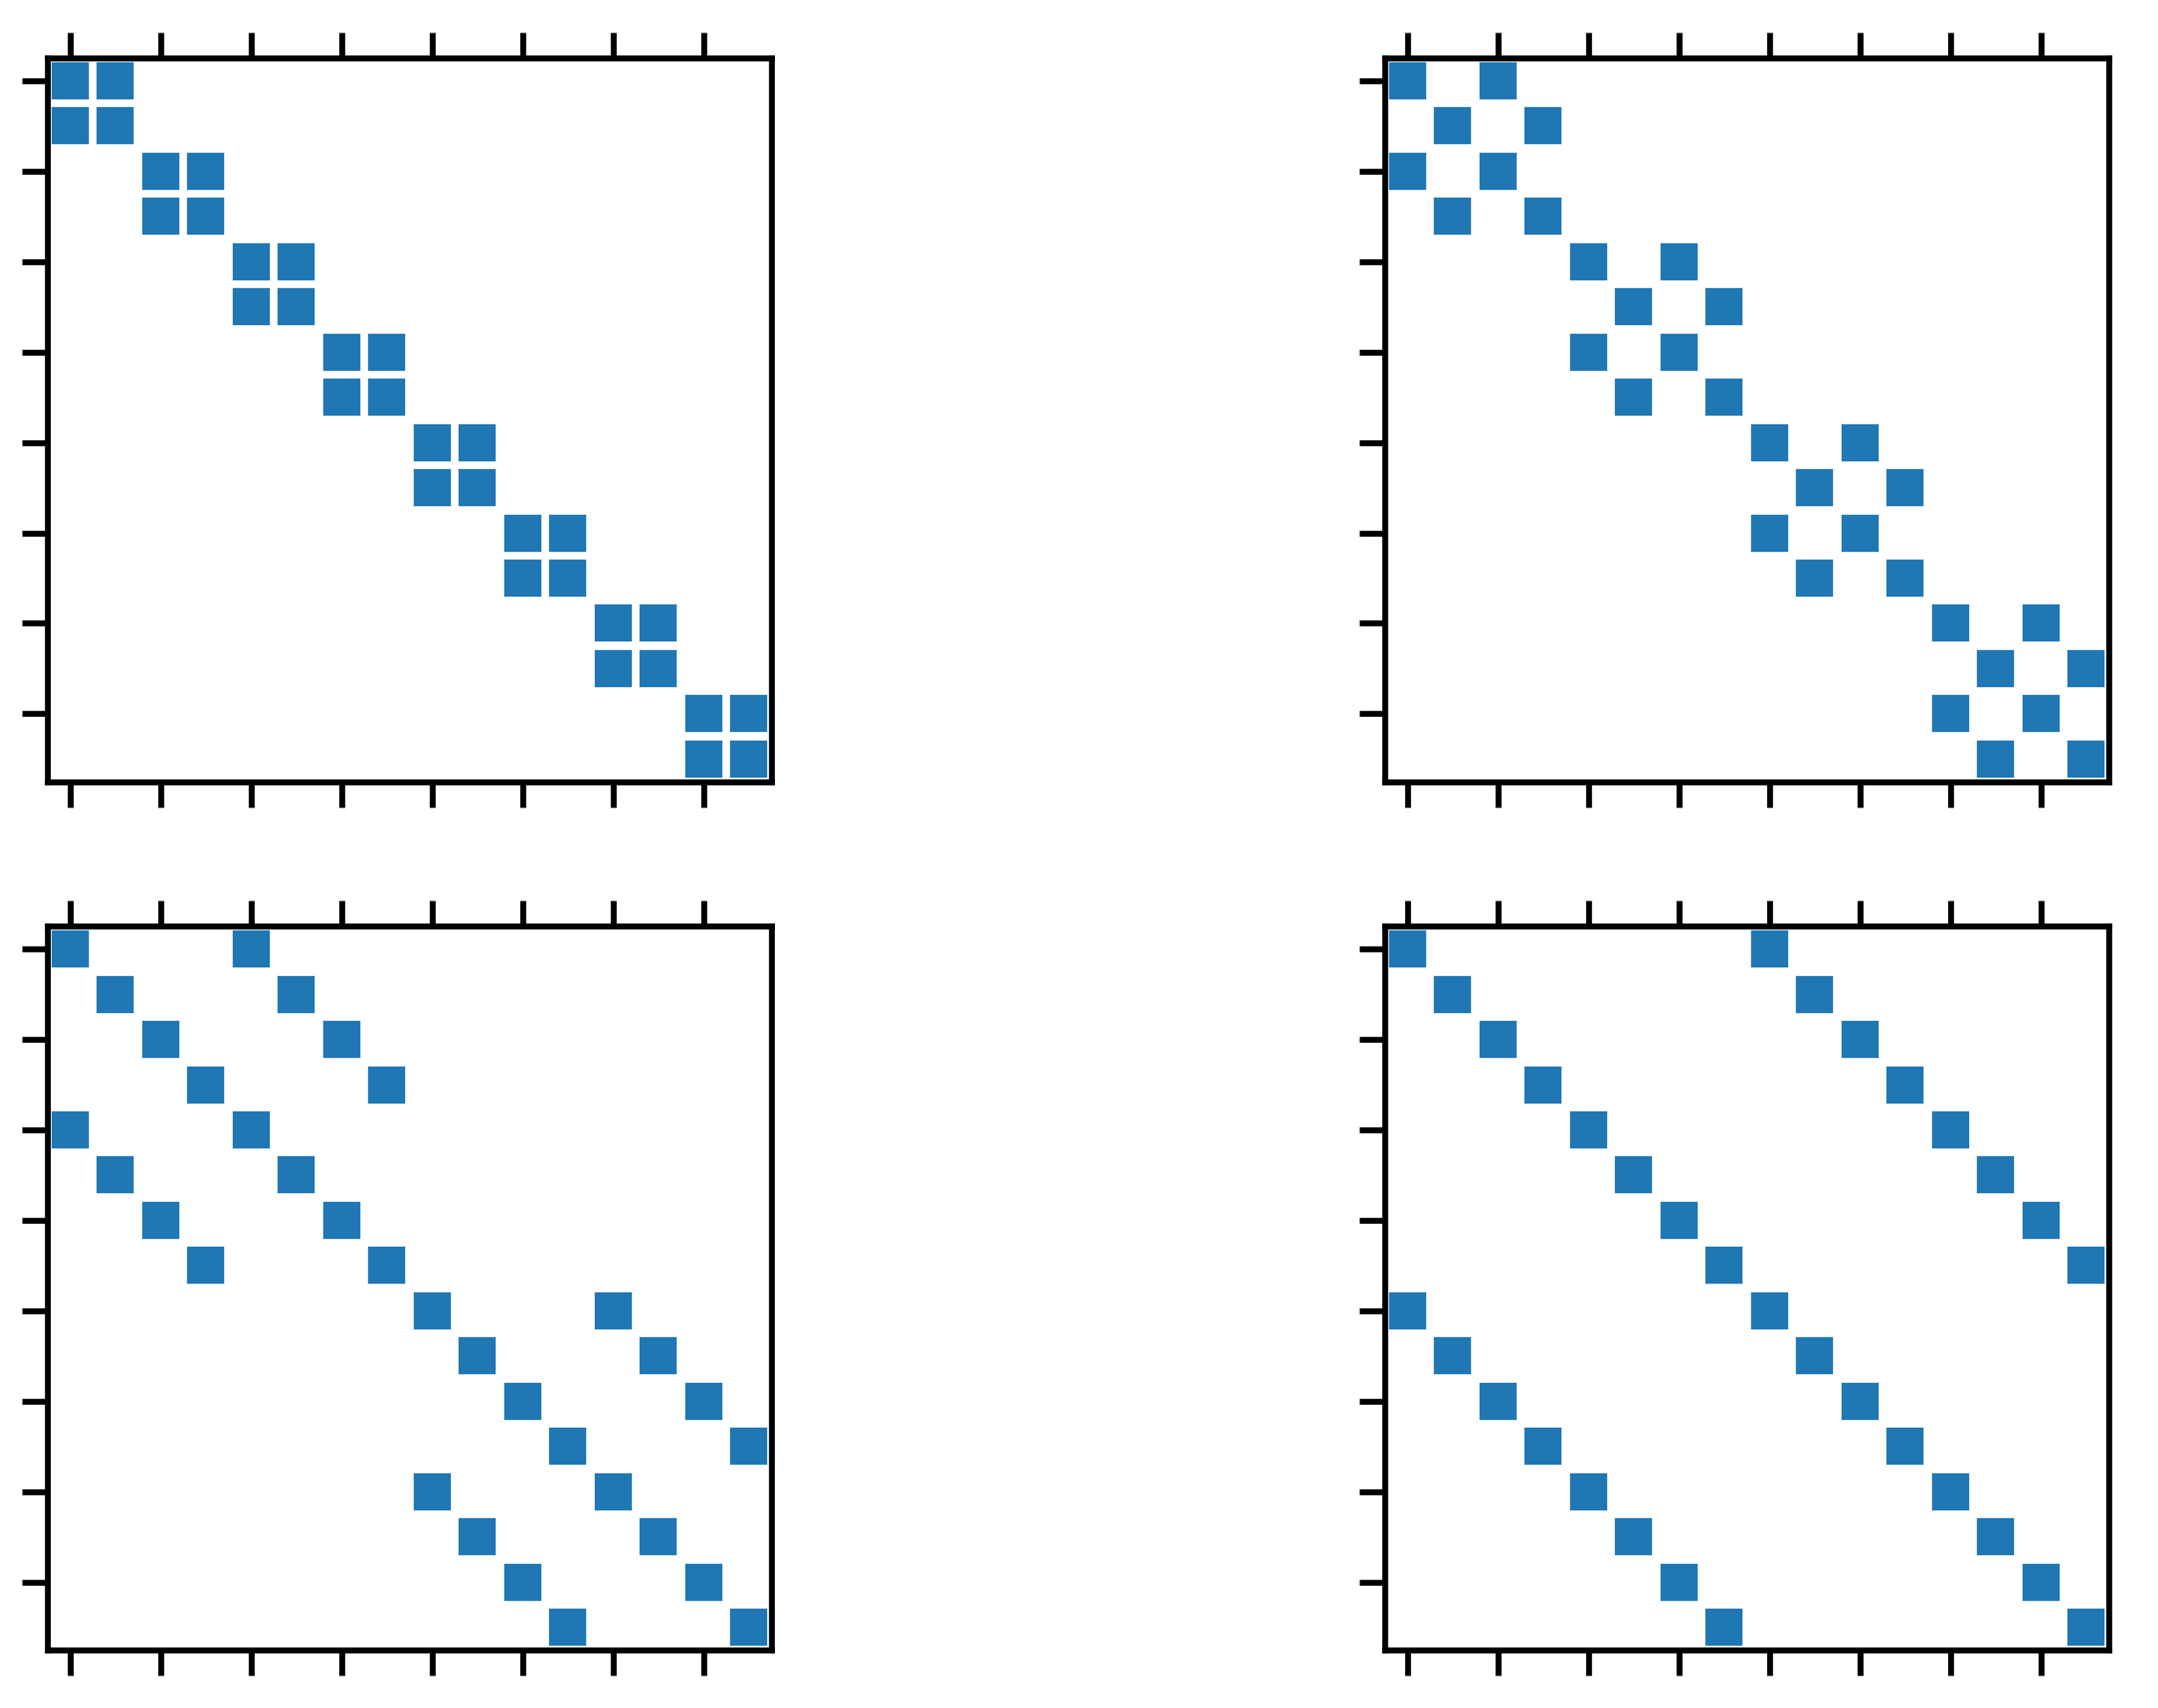
\includegraphics[width=0.575\linewidth]{figures/quadratures/b16.png}
\caption{}
\label{fig:factors}
\end{subfigure}
\hfill
\begin{subfigure}[t]{.5\textwidth}
\centering
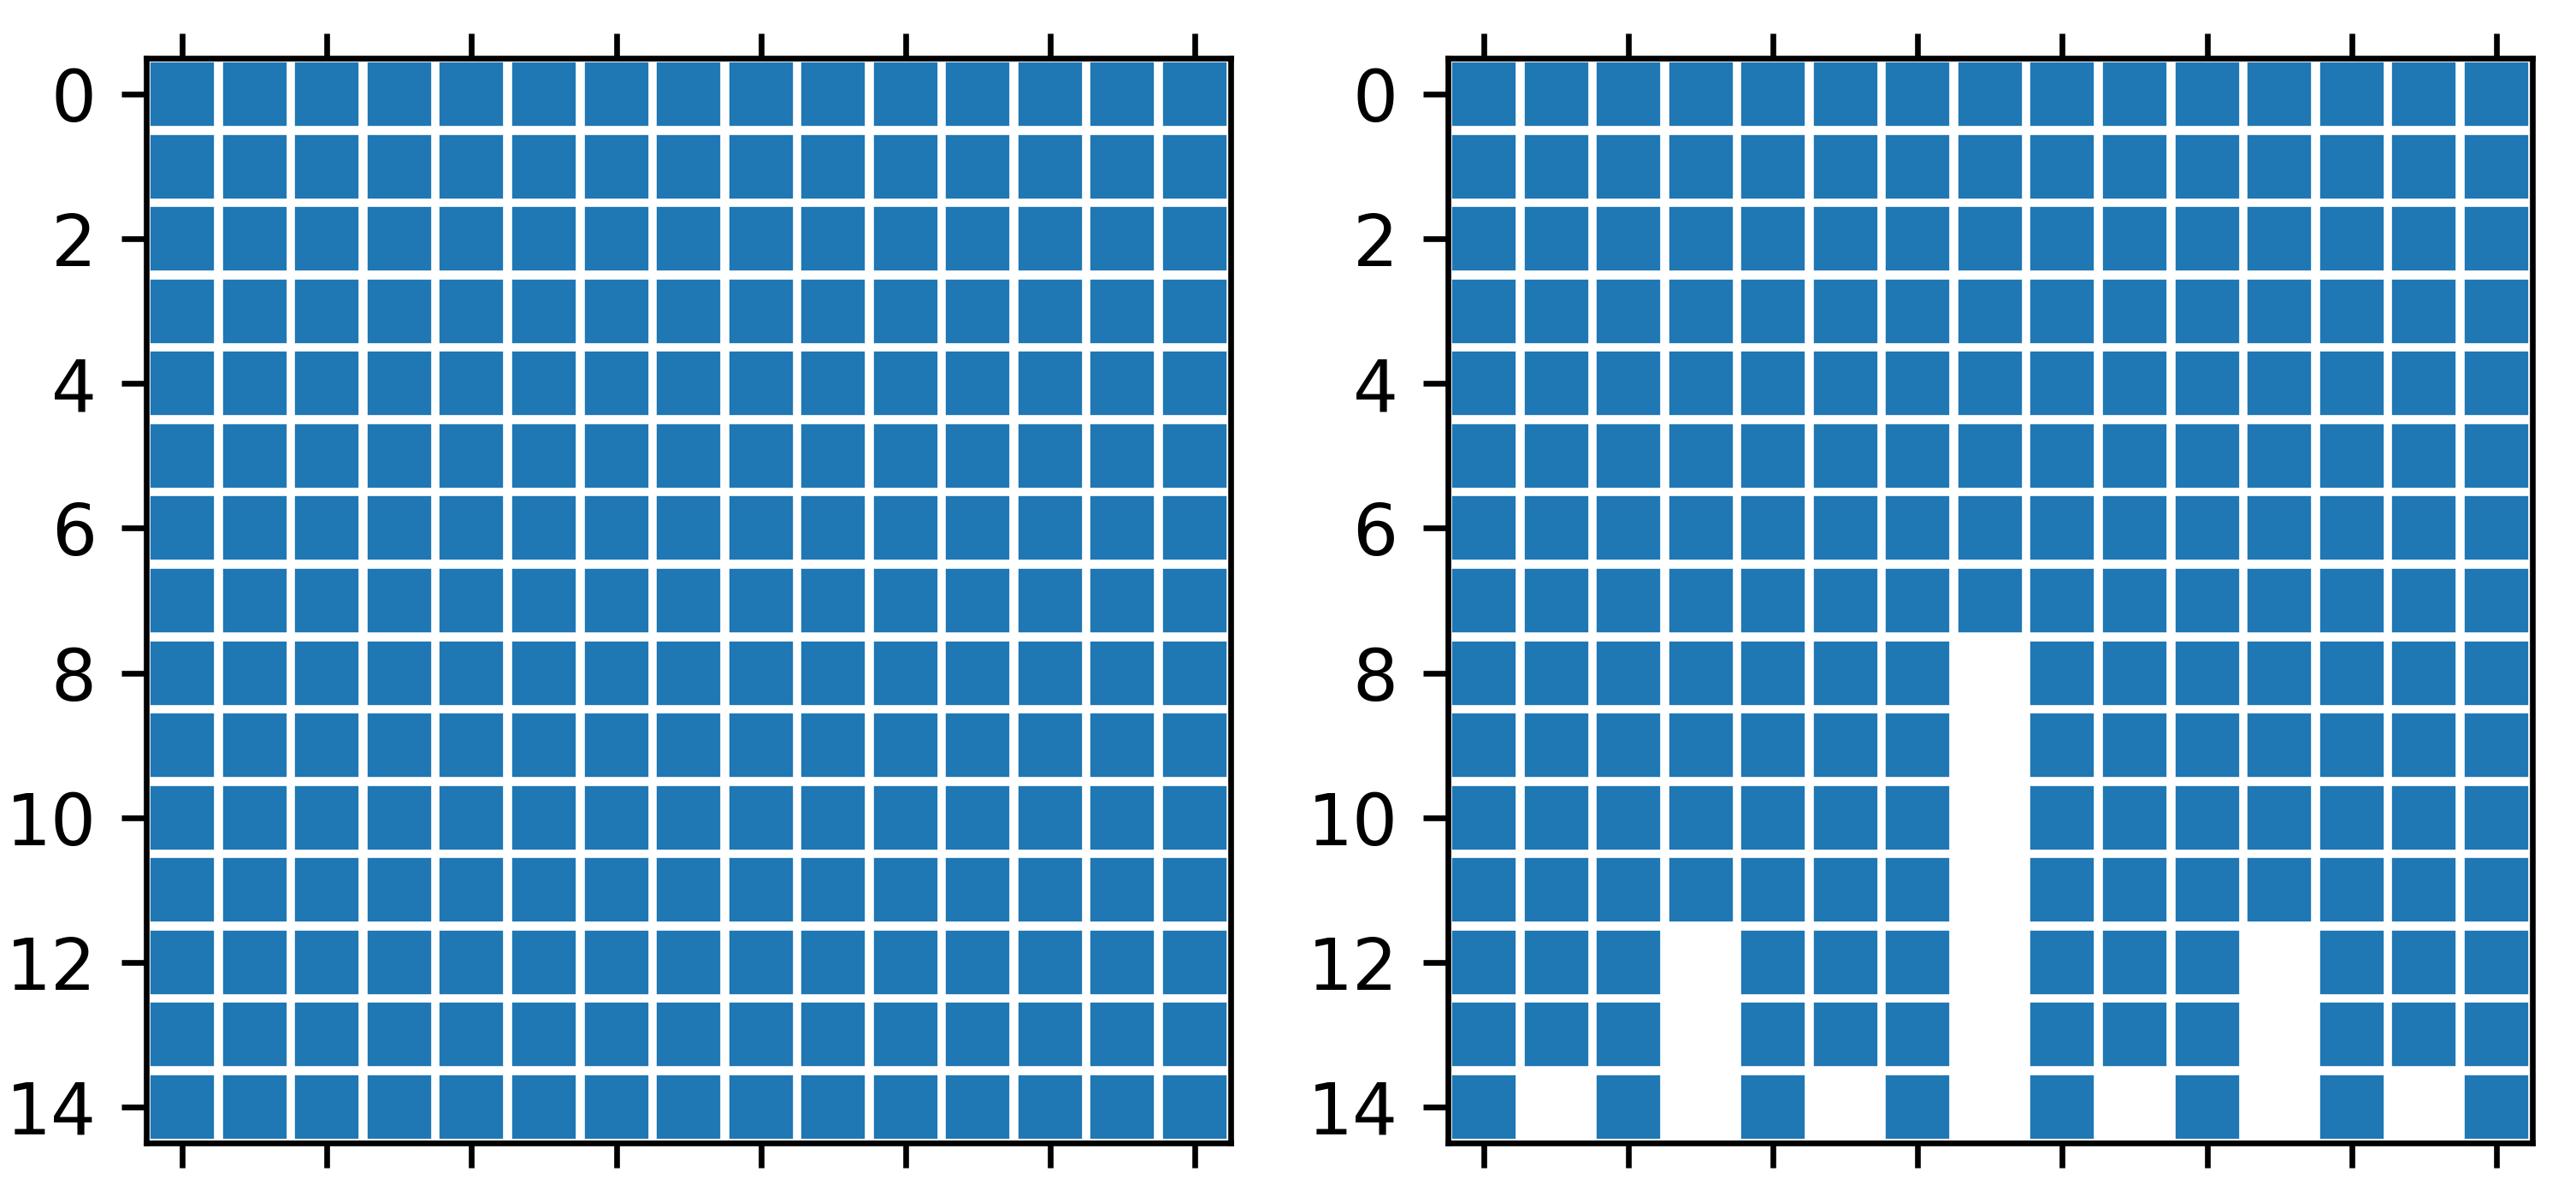
\includegraphics[width=\linewidth]{figures/quadratures/rvsr.png}
\caption{}
\label{fig:sparsity}
\end{subfigure}
\caption{(a) Butterfly orthogonal matrix factors for ${d = 16}$. (b) Sparsity pattern for $\mathbf{BPBPBP}$ (left) and $\mathbf{B}$ (right), $d=15$.}
\end{figure}


\section{Remarks on quadrature rules}
\paragraph*{Even functions.}
We note here that for specific functions~$f_{\mathbf{xy}}(\mathbf{w})$ we can derive better versions of $SR$ rule by taking on advantage of the knowledge about the integrand.
For example, the Gaussian kernel has ${f_{\mathbf{xy}}(\mathbf{w}) =
\cos(\mathbf{w}^{\boldsymbol{\top}}(\mathbf{x} - \mathbf{y}))}$.
Note that $f$ is even, so we can discard an excessive term in the summation in degree $(3, 3)$ rule, since $f(\mathbf{w}) = f(-\mathbf{w})$, i.e $SR^{3,3}$ rule reduces to
\begin{equation}
\begin{split}
\label{eq:sr33reduced}
SR^{3,3}_{\mathbf{Q}, \rho}(f) = &\left (1 - \sum_{j=1}^{d + 1}\frac{d}{(d + 1)\rho_j^2} \right )f(\mathbf{0}) + \frac{d}{d+1}\sum\limits_{j=1}^{d+1} \frac{f(\rho_j \mathbf{Qv}_j)}{\rho_j^2}.
\end{split}
\end{equation}

\paragraph*{Obtaining a proper \texorpdfstring{$\boldsymbol{\rho}$}.}
%%%%%%
It may be the case when sampling $\rho$ that $1 - \sum_{j = 1}^{d + 1}\frac{d}{(d + 1)\rho_j^2} < 0$ which results in complex $a_0$ term. Simple solution is just to resample $\rho_j$ to satisfy the non-negativity of the expression.
According to central limit theorem $\sum_{j = 1}^{d + 1} \frac{d}{(d + 1)\rho_j^2}$ tends to normal random variable with mean $1$ and variance $\frac{1}{d + 1}\frac{2}{d - 2}$.
The probability that this values is non-negative equals ${p = \mathbb{P}(1 - \sum_{j = 1}\frac{d}{(d + 1)\rho^2} \ge 0) \leadsto \frac12}$.
The expectation of number of resamples needed to satisfy non-negativity constraint is $\frac{1}{p}$ tends to 2.
%%%%%%


\section{Arc-cosine kernels}
\label{sub:arccos}
Arc-cosine kernels were originally introduced by \citep{cho2009kernel} upon studying the connections between deep learning and kernel methods. The integral representation of the $b^{th}$-order arc-cosine kernel is
\begin{equation*}
k_b(\mathbf{x}, \mathbf{y}) = 2 \int_{\mathbb{R}^n} \Theta(\mathbf{w}^{\boldsymbol{\top}}\mathbf{x})
                                                  \Theta(\mathbf{w}^{\boldsymbol{\top}}\mathbf{y})
                                                  (\mathbf{w}^{\boldsymbol{\top}}\mathbf{x})^b
                                                  (\mathbf{w}^{\boldsymbol{\top}}\mathbf{y})^b
                                                  p(\mathbf{w}) d\mathbf{w},
\end{equation*}
\begin{equation*}
k_b(\mathbf{x}, \mathbf{y}) = 2 \int_{\mathbb{R}^d} \phi_b(\mathbf{w}^{\boldsymbol{\top}}\mathbf{x})
\phi_b(\mathbf{w}^{\boldsymbol{\top}}\mathbf{y}) p(\mathbf{w}) d\mathbf{w},
\end{equation*}
where $\phi_b(\mathbf{w}^{\boldsymbol{\top}}\mathbf{x}) = \Theta(\mathbf{w}^{\boldsymbol{\top}}\mathbf{x}) (\mathbf{w}^{\boldsymbol{\top}}\mathbf{x})^b$, $\Theta(\cdot)$ is the Heaviside function
and $p$ is the density of the standard Gaussian distribution.
Such kernels can be seen as an inner product between the representation produced by infinitely wide single layer neural network with random Gaussian weights. They have closed form expressions in terms of the angle $\theta = \cos^{-1} \left( \frac{\mathbf{x}^{\boldsymbol{\top}}\mathbf{y}}{\|\mathbf{x}\|\|\mathbf{y}\|} \right)$ between %the objects $\mathbf{x}$ and $\mathbf{y}$.
$\mathbf{x}$ and $\mathbf{y}$.

Arc-cosine kernel of $0^{th}$-order shares the property of mapping the input on the unit hypersphere with RBF kernels, while order $1$ arc-cosine kernel preserves the norm as linear kernel (Gram matrix on original features):

These expressions for $0^{th}$-order and $1^{st}$-order arc-cosine kernels are given by
\[
k_0(\mathbf{x},\mathbf{y}) = 1 - \frac{\theta}{\pi},\qquad k_1(\mathbf{x},\mathbf{y}) = \frac{\|\mathbf{x}\|\|\mathbf{y}\|}{\pi}(\sin\theta + (\pi - \theta)\cos\theta).
\]
The $0$-order arc-cosine kernel is given by ${k_0(\mathbf{x},\mathbf{y}) = 1 - \frac{\theta}{\pi}}$, the $1$-order kernel is given by ${k_1(\mathbf{x},\mathbf{y}) = \frac{\|\mathbf{x}\|\|\mathbf{y}\|}{\pi}(\sin\theta + (\pi - \theta)\cos\theta)}$.

Let
${\phi_0(\mathbf{w}^{\boldsymbol{\top}}\mathbf{x}) = \Theta(\mathbf{w}^{\boldsymbol{\top}}\mathbf{x})}$,
${\phi_1(\mathbf{w}^{\boldsymbol{\top}}\mathbf{x}) = \max (0, \mathbf{w}^{\boldsymbol{\top}}\mathbf{x})}$. We now can rewrite the integral representation as follows:
\begin{align*}
k_{b}(\mathbf{x},\mathbf{y}) &= 2 \int\limits_{\mathbb{R}^d}  \phi_b(\mathbf{w}^{\boldsymbol{\top}}\mathbf{x}) \phi_b(\mathbf{w}^{\boldsymbol{\top}}\mathbf{y}) p(\mathbf{w}) d\mathbf{w} \approx \frac{2}{n} \sum\limits_{i=1}^n SR_{\mathbf{Q}_i,\boldsymbol{\rho}_i}^{3,3}.
\end{align*}
For arc-cosine kernel of order $0$ the value of the function $\phi_0(0) = \Theta(0) = 0.5$ results in
\begin{equation*}
\begin{split}
SR^{3,3}_{\mathbf{Q}, \rho}(f) = & 0.25 \left (1 - \sum_{j = 1}^{d + 1}\frac{d}{(d + 1)\rho_j^2} \right ) + \frac{d}{d+1}\sum\limits_{j=1}^{d+1} \frac{f(\rho_j \mathbf{Qv}_j) + f(-\rho_j \mathbf{Qv}_j)}{2\rho^2}.
\end{split}
\end{equation*}
In the case of arc-cosine kernel of order $1$, the value of $\phi_1(0)$ is $0$ and the $SR^{3,3}$ rule reduces to
\begin{equation*}
SR^{3,3}_{\mathbf{Q}, \rho}(f) = \frac{d}{d+1}\sum\limits_{j=1}^{d+1} \frac{f(|\rho \mathbf{Qv}_j|)}{2\rho_j^2}.
\end{equation*}
\chapter{Additional results for Score Matching}

\section{Technical Results}
\label{chap:Technical}

\subsection{Exact solution for the Kernel Denoising Score Matching with RFF}
\label{sec:exact_solution}
We start with the first order optimality condition:
\begin{equation*}
    \int p_{\varepsilon}({\bf y}) A^*({\bf y})\nabla V(A({\bf y})f)d{\bf y} + \lambda f = 0,
\end{equation*}
where $A^*({\bf y}): \mathbb{R}^m \to \mathcal{H}$ is an adjoint to $A({\bf y})$ and
$A^*({\bf y}){\bm \alpha} = \sum_{i = 1}^m \alpha_i\phi_i({\bf y}, \cdot)$.
Denoting
\begin{align*}
    &{\bm \alpha}({\bf y}) = -\frac{1}{\lambda}\nabla V(A({\bf y})f),\quad f = \int p_{\varepsilon}({\bf y})A^*({\bf y}){\bm \alpha}({\bf y})d {\bf y},
\end{align*}
the first order optimality condition could be rewritten as an integral equation on
${\bm \alpha}({\bf y})$:
\begin{equation}
    {\bm \alpha}({\bf y}) = -\frac{1}{\lambda}\nabla V\left(\int p_{\varepsilon}({\bf z})A({\bf y})A^*({\bf z})\alpha({\bf z})d{\bf z}\right),
\end{equation}
where $A({\bf y})A^*({\bf z})\alpha({\bf z}) = \sum\limits_{i = 1}^m\alpha_i({\bf z})\{\langle \phi_j({\bf y}, \cdot),  \phi_i({\bf z}, \cdot)\rangle\}_{j = 1}^m = {\bm K}({\bf y}, {\bf z}){\bm \alpha}({\bf z})$.

The gradient of $V$ is given
by~$\nabla V = (\frac{1}{n}, \frac{1}{n}, \ldots, \frac{1}{n}, 1)^{\top}$.
Then, we have ${\bm \alpha}({\bf y}) = ({\bm \beta}^{\top}({\bf y}), \delta)^{\top}$,
where $\delta = -\frac{1}{\lambda}$.
The integral equation on ${\bm \beta}({\bf y})$ can be expressed as
\begin{equation}
    {\bm \beta}({\bf y}) = -\frac{1}{n\lambda}\int p_{\varepsilon}({\bf z})\hat{A}({\bf y})\hat{A}({\bf z})^*{\bm \beta}({\bf z})d{\bf z} + \frac{1}{n\lambda^2}\int p_{\varepsilon}({\bf z}) \hat{A}({\bf y}) \phi_m({\bf z}, \cdot)d{\bf z},
\end{equation}
where $(\hat{A}({\bf y})f)_i = (A({\bf y})f)_i$, $i = 1, \ldots, m - 1$.
Let $b = \int p_{\varepsilon}({\bf y})\phi_m({\bf y}, \cdot) d {\bf y}$ and
$C = \int p_{\varepsilon}({\bf y})\hat{A}^*({\bf y}){\bm \beta}({\bf y}) d {\bf y}$.
Then we search for the solution of \eqref{eq:beta_integal} in the form
${\bm \beta}({\bf y}) = -\frac{1}{n\lambda}\hat{A}({\bf y})C + \frac{1}{n\lambda^2}\hat{A}({\bf y})b$.
In this case we have
\begin{equation*}
    \hat{A}({\bf y})\left[C + \frac{1}{n\lambda}BC - \frac{1}{n\lambda^2}Bb\right] = 0,
\end{equation*}
where $B = \int p_{\varepsilon}({\bf y})\hat{A}^*({\bf y})\hat{A}({\bf y}) d{\bf y}$ and
$b \in \mathcal{H}$ is a convolution of $\phi_m$ and noise density $p_{\varepsilon}$.
% Indeed, fixing ${\bf z}$, $\phi_m({\bf y, z}) \in H$ as a function of ${\bf y}$. Then ${\cal F}[\phi_m({\bf y, z}) * p_{\varepsilon}({\bf y})] = {\cal F}[\phi_m({\bf y, z})]{\cal F}[p_{\varepsilon}({\bf y})]$.
% $$\int \frac{|{\cal F}[\phi_m({\bf y, z})]{\cal F}[p_{\varepsilon}({\bf y})]|^2}{{\cal F}[k](w)}dw \leq \sup|{\cal F}[p_{\varepsilon}({\bf y})]|^2\int \frac{|{\cal F}[\phi_m({\bf y, z})]|^2}{{\cal F}[k](w)}dw < \infty$$
% The last follow $p_{\varepsilon}({\bf y}) \in L^1$.

%As produnct of function from $H$ belongs to $H$
Solution $C^*$ of the above equation provides ${\bm \beta}^*({\bf y})$ and, as a result,
the solution to the initial problem.
Let us show that the obtained estimator belongs to $H$.
In fact, since
\[
    C + \frac{1}{n\lambda}BC - \frac{1}{n\lambda^2}Bb \in {\rm Ker}\hat{A}({\bf y}) \subseteq
    \mathcal{H}
\]
and $B + n\lambda I$ is continuously invertible we have that $C^* \in \mathcal{H}$.
Finally, we have
\[
    f^* = B\left[-\frac{1}{n\lambda}C^* + \frac{1}{n\lambda^2}b\right] = C^* - \frac{1}{\lambda}b - \gamma \in \mathcal{H},
\]
where we assume $\gamma \in {\rm Ker}\hat{A}({\bf y})$.



\subsection{RFF solution derivation}
\label{sec:rff_solution_derivation}
Let us use the expressions for the solution without noise
(here for simplicity the term with $\partial_i \log q_0({\bf x}_a)$ is omitted):
\begin{equation*}
    \left [ \hat{A}({\bf 0})\hat{A}({\bf 0})^* \right ]_{(a - 1)d + i, (b - 1)d + j} =
    \partial_i\partial_{j + d}k({\bf x}_a, {\bf x}_b),~\quad a, b \in [n],~i, j \in [d],
\end{equation*}
\begin{equation*}
    \left [ \hat{A}({\bf 0}){\bm \phi}_m({\bf 0}, \cdot) \right ]_{(a - 1)d + i} =
    \frac{1}{n}\sum_{b, j = 1}^{n, d}\partial_i\partial^2_{j + d}k({\bf x}_a, {\bf x}_b),~\quad a\in [n],~i \in [d].
\end{equation*}
Then we have
$\hat{A}({\bf y})\hat{A}({\bf z})^* \approx \partial{\bm \Phi}_y\partial{\bm \Phi}_z^{\top}$
and
$\hat{A}({\bf y}){\bm \phi}_m({\bf z}, \cdot) * p_{\varepsilon}({\bf z}) \approx \frac{1}{n}
\partial{\bm \Phi}_y(\partial^2{\bm \Phi}_z * p_{\varepsilon}({\bf z}))^{\top}{\bf 1}$.

Now we have everything to obtain RFF approximation of \eqref{eq:beta_finite_sample}:
\begin{align*}
    {\bm \beta}_K = -\frac{1}{nK\lambda}\partial {\bm \Phi}_K\partial {\bm \Phi}_K^{\top}{\bm \beta}_K  + \frac{1}{n^2\lambda^2}\partial{\bm \Phi}_K \odot (\partial^2 {\bm \Phi}_z * p({\bf z}))^{\top}{\bf 1},
\end{align*}
where
\[  \partial {\bm \Phi}_K =
    \begin{bmatrix}
        {\bm \Phi}_{z_1}\\
        \vdots\\
        {\bm \Phi}_{z_K}
    \end{bmatrix}, \quad
    \partial{\bm \Phi}_K \odot (\partial^2 {\bm \Phi}_z * p({\bf z}))^{\top}{\bf 1} =
    \begin{bmatrix}
        \partial{\bm \Phi}_{z_1}(\partial^2 {\bm \Phi}_z * p({\bf z}))^{\top}{\bf 1}\\
        \vdots\\
        \partial{\bm \Phi}_{z_K}(\partial^2 {\bm \Phi}_z * p({\bf z}))^{\top}{\bf 1}
    \end{bmatrix}.
\]
Denoting
\begin{equation*}
    {\bm h} = \frac{1}{n}(\partial^2 {\bm \Phi}_z * p({\bf z}))^{\top}{\bf 1},
    \quad
    {\bm H} =
    \int p_{\varepsilon}({\bf y})\partial{\bm \Phi}_y^{\top}\partial{\bm \Phi}_y d{\bf y}
\end{equation*}
we obtain the following expression for the descretized solution $f_K$:
\begin{align*}
    f_K
    &= \frac{1}{n\lambda^2}{\bm \phi}(\cdot)^{\top}{\bm H} \left[-\frac{1}{K}\partial {\bm \Phi}_K^{\top}\left(\frac{1}{K}\partial {\bm \Phi}_K\partial {\bm \Phi}_K^{\top} + n\lambda {\bf I}\right)^{-1}\partial{\bm \Phi}_K \odot {\bm h} + {\bm h}\right]
   -\frac{1}{\lambda} {\bm \phi}(\cdot)^{\top}{\bm h}\\
    &= \frac{1}{n\lambda^2}{\bm \phi}(\cdot)^{\top}{\bm H}
    \left[-\frac{1}{K}\left(\frac{1}{K}\partial  {\bm \Phi}_K^{\top}\partial{\bm \Phi}_K + n\lambda {\bf I}\right)^{-1}\partial {\bm \Phi}_K^{\top}\partial{\bm \Phi}_K \odot {\bm h} + {\bm h}\right]
    -\frac{1}{\lambda} {\bm \phi}(\cdot)^{\top}{\bm h}.
\end{align*}
By taking a limit over $K \to \infty$, and using
${\bm H} = \lim\limits_{K \to \infty}\frac{1}{K}\partial {\bm \Phi}_K^{\top}\partial{\bm\Phi}_K$ alond with
\begin{equation*}
    \lim\limits_{K \to \infty}(n\lambda{\bf I} + \frac{1}{K}\partial {\bm \Phi}^{\top}_K\partial {\bm \Phi}_K) \lim\limits_{K \to \infty}\frac{1}{K}\partial {\bm \Phi}^{\top}_K{\bm \beta}_K = \lim\limits_{K \to \infty}\frac{1}{K\lambda}\partial {\bm \Phi}^{\top}_K\partial {\bm \Phi}_K{\bm h}
\end{equation*}
the solution $f^*$ is given:
\begin{align*}
    f_{m}^* = \lim\limits_{K \to \infty} f_K
    &= -\frac{1}{n\lambda^2}{\bm\phi}(\cdot)^{\top}{\bm H}({\bm H} +
    n \lambda {\bf I})^{-1}{\bm Hh} + \frac{1}{n\lambda^2}{\bm \phi}(\cdot)^{\top}{\bm Hh} -
    \frac{1}{\lambda}{\bm \phi}(\cdot)^{\top}{\bm h}\nonumber\\
    &= \frac{1}{\lambda}{\bm \phi}(\cdot)^{\top}({\bm H} + n\lambda{\bf I})^{-1}{\bm Hh}
    - \frac{1}{\lambda}{\bm \phi}(\cdot)^{\top}{\bm h},
\end{align*}
where index $m$ refers to the number of RFF features.




\subsection{Proof for the error bounds of score matching with RFF}
\label{sec:error_bound_proof}
The idea of the proof is to upper bound the expected square difference between solutions:
\begin{equation}
    \mathbb{E}_{{\bf x}, {\bf w}}(f_{n, m}^*({\bf x}) - f_n^*({\bf x}))^2,
\end{equation}
where the difference between RFF and exact kernel solutions ($f_{n, m}^*,~f_n^*$)
is expressed as follows:
\begin{align*}
    f_{n, m}^* - f_n^*
    &= -\frac{1}{\lambda n}\partial^2{\bm k}(\cdot)^{\top}{\bf 1}
    + \frac{1}{\lambda n} {\bm \phi}^{\top}(\cdot)\partial^2\bm{\Phi}^{\top}{\bf 1} \\
    &+ \frac{1}{\lambda n}\partial{\bm k}(\cdot)^{\top}(\partial\partial {\bm K} +
    \lambda n{\bf I})^{-1}\partial\partial^2 {\bm K}{\bf 1}
    -\frac{1}{\lambda n}{\bm \phi}^{\top}(\cdot)\partial\bm{\Phi}^{\top}(\partial\bm{\Phi}
    \partial\bm{\Phi}^{\top} +
    \lambda n {\bf I})^{-1}\partial\bm{\Phi}\partial^2\bm{\Phi}^{\top}{\bf 1} \\
    &= \frac{1}{\lambda n}(\partial^2\bm{\Phi}{\bm \phi}(\cdot) -
    \partial^2{\bm k}(\cdot))^{\top}{\bf 1}
    + \frac{1}{\lambda n}(\partial{\bm k}(\cdot) -
    \partial\bm{\Phi}{\bm \phi}(\cdot))^{\top}(\partial\partial {\bm K} +
    \lambda n{\bf I})^{-1}\partial\partial^2 {\bm K}{\bf 1} \\
    &+ \frac{1}{\lambda n}{\bm \phi}^{\top}(\cdot)\partial\bm{\Phi}^{\top} \left[
        (\partial\partial {\bm K} + \lambda n{\bf I})^{-1} -
        (\partial\bm{\Phi}\partial\bm{\Phi}^{\top} + \lambda n {\bf I})^{-1}
    \right] \partial\partial^2 {\bm K}{\bf 1} \\
    &+ \frac{1}{\lambda n}{\bm \phi}^{\top}(\cdot)\partial\bm{\Phi}^{\top}(\partial\bm{\Phi}
    \partial\bm{\Phi}^{\top} + \lambda n {\bf I})^{-1}(\partial\partial^2 {\bm K} -
    \partial\bm{\Phi}\partial^2\bm{\Phi}^{\top}){\bf 1}.
\end{align*}
The above expectation is taken jointly over random Fourier weights and given points
${\bf x} \sim p_0$.
It can be written as
$\mathbb{E}_{{\bf x}, {\bf w}}[f] = \mathbb{E}_{{\bf w}}\mathbb{E}_{{\bf x}}[f | {\bf w}]$.
The first term in the above expression is the difference between $\hat{\xi}$
and its RFF approximation $\hat{\xi}_m$, so, we have:
\begin{align*}
    \mathbb{E}_{{\bf w}}{\bf 1}^{\top}&(\partial^2\bm{\Phi}{\bm \phi}(\cdot) - \partial^2{\bm k}(\cdot))(\partial^2\bm{\Phi}{\bm \phi}(\cdot) - \partial^2{\bm k}(\cdot))^{\top}{\bf 1} \\
    &= {\bf 1}^{\top}\left[\mathbb{E}_{{\bf w}}[\partial^2\bm{\Phi}{\bm \phi}(\cdot){\bm \phi}(\cdot)^{\top}\partial^2\bm{\Phi}^{\top}] - \partial^2{\bm k}(\cdot)\partial^2{\bm k}(\cdot)^{\top}\right]{\bf 1}\\
    &\leq \frac{m - 1}{m}{\bf 1}^{\top}\partial^2{\bm k}(\cdot)\partial^2{\bm k}^{\top}(\cdot){\bf 1} + \frac{1}{m}{\bf 1}^{\top}\partial^2\partial^2{\bm K}{\bf 1} - {\bf 1}^{\top}\partial^2{\bm k}(\cdot)\partial^2{\bm k}(\cdot)^{\top}{\bf 1}\\
    &\leq \frac{1}{m}{\bf 1}^{\top}\partial^2\partial^2{\bm K}{\bf 1},
\end{align*}
where the first inequality is obtained using
$\sup_{\bf x}|\phi_i({\bm W}{\bf x} + {\bm b})| \leq 1$.
As this expression does not depend on ${\bf x}$, the joint expectation will be the same.

For the second term in $f_{n, m}^*({\bf x}) - f_n^*({\bf x})$ derivation of the
upper bound is technically the same, but with lower-order derivatives, so
\begin{align*}
    \mathbb{E}_{{\bf w}}\left[(\partial{\bm k}(\cdot) -
    \partial\bm{\Phi}{\bm \phi}(\cdot))^{\top}(\partial\partial {\bm K} +
    \lambda n{\bf I})^{-1}\partial\partial^2 {\bm K}{\bf 1}\right]^2 \leq \\
    \frac{1}{m}\|\partial\partial {\bm K}^{\frac{1}{2}}(\partial\partial {\bm K} + \lambda n{\bf I})^{-1}\partial\partial^2 {\bm K}{\bf 1}\|^2.
\end{align*}

Third them:
\begin{align*}
    \mathbb{E}_{{\bf x, w}}&\left[{\bm \phi}^{\top}(\cdot)\partial\bm{\Phi}^{\top}\left[(\partial\partial {\bm K} + \lambda n{\bf I})^{-1} - (\partial\bm{\Phi}\partial\bm{\Phi}^{\top} + \lambda n {\bf I})^{-1}\right]\partial\partial^2 {\bm K}{\bf 1}\right]^2 \\
    &= \mathbb{E}_{{\bf x, w}}\left[{\bm \phi}^{\top}(\cdot)\partial\bm{\Phi}^{\top}(\partial\bm{\Phi}\partial\bm{\Phi}^{\top} + \lambda n{\bf I})^{-1}(\partial\partial {\bm K} - \partial\bm{\Phi}\partial\bm{\Phi}^{\top})(\partial\partial {\bm K} + \lambda n {\bf I})^{-1}\partial\partial^2 {\bm K}{\bf 1}\right]^2\\
    &\leq \mathbb{E}_{{\bf w}}\mathbb{E}_{{\bf x}}\left[\|{\bf R}\|_2 \|(\partial\partial {\bm K} - \partial\bm{\Phi}\partial\bm{\Phi}^{\top})(\partial\partial {\bm K} + \lambda n {\bf I})^{-1}\partial\partial^2 {\bm K}{\bf 1}\|^2 | {\bf w}\right],
\end{align*}
where only $\bf R$ depends on ${\bf x}$.
\begin{align*}
    \mathbb{E}_{\bf x}{\bf R}
    &= (\partial\bm{\Phi}\partial\bm{\Phi}^{\top} + \lambda n{\bf I})^{-1}\partial\bm{\Phi}
    \mathbb{E}_{\bf x}\left[{\bm \phi}(\cdot){\bm \phi}^{\top}(\cdot)\right]\partial\bm{\Phi}^{\top}(\partial\bm{\Phi}\partial\bm{\Phi}^{\top} + \lambda n{\bf I})^{-1}\\
    &= \frac{1}{n} (\partial\bm{\Phi}\partial\bm{\Phi}^{\top} + \lambda n{\bf I})^{-1}\partial\bm{\Phi}
    (\bm{\Phi}^{\top}\bm{\Phi} + \varepsilon n I)\partial\bm{\Phi}^{\top}(\partial\bm{\Phi}\partial\bm{\Phi}^{\top} + \lambda n{\bf I})^{-1}
\end{align*}
This inequality holds with probability $1 - \delta$ for
$n \geq \frac{8}{3\varepsilon^2} \log\frac{m}{\delta}$
%$n \geq \frac{8 \sup_{\bf x}k({\bf x}, {\bf x})}{3\varepsilon^2} \log\frac{m}{\delta}$
and obtained from the Bernstein inequality assuming that the weights are fixed \cite{Tropp_2015}.
\begin{align*}
    \lambda_{\max}({\bf R})
    &= \frac{1}{n}\lambda_{\max}\left[(\partial\bm{\Phi}\partial\bm{\Phi}^{\top} +
    \lambda n{\bf I})^{-1}\partial\bm{\Phi}
    (\bm{\Phi}^{\top}\bm{\Phi} + n\varepsilon I)\partial\bm{\Phi}^{\top}(\partial\bm{\Phi}
    \partial\bm{\Phi}^{\top} + \lambda n{\bf I})^{-1}\right]\\
    &\leq \frac{1}{n}\lambda_{\max}\left[(\bm{\Phi}^{\top}\bm{\Phi} + n\varepsilon I)
    \partial\bm{\Phi}^{\top}(\partial\bm{\Phi}\partial\bm{\Phi}^{\top} + \lambda n{\bf I})^{-1}\partial\bm{\Phi}
    \right]\\
    &\leq \frac{1}{n}\lambda_{\max}\left[(\bm{\Phi}^{\top}\bm{\Phi} + n\varepsilon I)\right] \leq
    \frac{1}{n}{\rm tr}\left[(\bm{\Phi}^{\top}\bm{\Phi} + n\varepsilon I)\right] \\
    &\leq \left(\frac{1}{m}\max_i\sup_{\bf x}\|\phi_i({\bm W}{\bf x} + {\bm b})\|^2 +
    \varepsilon\right) \leq \frac{1}{m} + \varepsilon
\end{align*}
\begin{align*}
    \mathbb{E}_{\bf w}&\|(\partial\partial {\bm K} - \partial\bm{\Phi}\partial\bm{\Phi}^{\top})(\partial\partial {\bm K} + \lambda n {\bf I})^{-1}\partial\partial^2 {\bm K}{\bf 1}\|^2\\
    & = {\bf 1}^{\top}\partial\partial^2 {\bm K}^{\top}(\partial\partial {\bm K} + \lambda n {\bf I})^{-1}(\mathbb{E}_{\bf w}\partial\bm{\Phi}\partial\bm{\Phi}^{\top}\partial\bm{\Phi}\partial\bm{\Phi}^{\top} - \partial\partial {\bm K}^2)(\partial\partial {\bm K} + \lambda n {\bf I})^{-1}\partial\partial^2 {\bm K}{\bf 1}
\end{align*}
\begin{align*}
    \mathbb{E}_{\bf w}\partial\bm{\Phi}\partial\bm{\Phi}^{\top}\partial\bm{\Phi}\partial\bm{\Phi}^{\top} = \frac{m - 1}{m} \partial\partial {\bm K}^2 + \frac{1}{m}{\bf D}_1
\end{align*}
where the latter term is obtained under assumption that ${\bf D}_1$ does not depend on
${\bf x}$.
This assumption holds for a sufficiently smooth kernels and we can
rewrite the expression under an expectation as polynomial of weights times
trigonometric function.
\begin{align*}
    \mathbb{E}_{\bf w}&\|(\partial\partial {\bm K} - \partial\bm{\Phi}\partial\bm{\Phi}^{\top})(\partial\partial {\bm K} + \lambda n {\bf I})^{-1}\partial\partial^2 {\bm K}{\bf 1}\|^2
    \leq \frac{1}{m}\|{\bf D}_1^{\frac{1}{2}}(\partial\partial {\bm K} + \lambda n {\bf I})^{-1}\partial\partial^2 {\bm K}{\bf 1}\|^2
\end{align*}
Analogously, for the last term under assumption that ${\bf D}_2 < \infty$ we have
\begin{align*}
    \mathbb{E}_{{\bf x, w}} \partial\bm{\Phi}\partial^2\bm{\Phi}^{\top}\partial\bm{\Phi}\partial^2\bm{\Phi}^{\top} \leq \frac{1}{m}\|{\bf D}_2^{\frac{1}{2}}{\bf 1}\|^2.
\end{align*}

Finally, combining all the above, we have
\begin{align*}
    \mathbb{E}_{{\bf x}, {\bf w}}(f_{n, m}^*({\bf x}) - f_n^*({\bf x}))^2 \leq \frac{2}{\lambda^2 n^2 m^2}\left[
    m{\bf 1}^{\top}\partial^2\partial^2{\bm K}{\bf 1} + m\|\partial\partial {\bm K}^{\frac{1}{2}}(\partial\partial {\bm K} + \lambda n{\bf I})^{-1}\partial\partial^2 {\bm K}{\bf 1}\|^2 \right. \nonumber \\
    \left. + (1 + \varepsilon m)\|{\bf D}_2^{\frac{1}{2}}{\bf 1}\|^2 + (1 + \varepsilon m)\|{\bf D}_1^{\frac{1}{2}}(\partial\partial {\bm K} + \lambda n {\bf I})^{-1}\partial\partial^2 {\bm K}{\bf 1}\|^2
    \right].
\end{align*}



\subsection{Derivation of \texorpdfstring{${\bm H}$ and ${\bm h}$ for }
 GGaussian noise}
\label{sec:Hh_der}
    \begin{align*}
        {\bm H}
        &= \partial \Phi^{\top}\partial \Phi * p_{\varepsilon}\\
        &= \sum\limits_{a = 1}^n\sum\limits_{i = 1}^d \partial_i \phi(\bm{W}{\bf x}_a + \bm{b})\partial_i \phi^{\top}(\bm{W}{\bf x}_a + \bm{b}) * p_{\varepsilon}\\
        &= \sum\limits_{a = 1}^n\sum\limits_{i = 1}^d \bm{W}_{:, i}\bm{W}_{:, i}^\top \odot \phi'(\bm{W}{\bf x}_a + \bm{b}) \phi'^\top(\bm{W}{\bf x}_a + \bm{b}) * p_{\varepsilon}\\
        &= \frac{1}{M}\bm{W}\bm{W}^{\top} \odot \sum\limits_{a = 1}^n \sin(\bm{W}{\bf x}_a + \bm{b}) \sin^\top(\bm{W}{\bf x}_a + \bm{b}) * p_{\varepsilon}
        \label{eq:H_derivation}
    \end{align*}
    Assuming that $p_{\varepsilon} = {\cal N}({\bf 0}, \sigma^2{\bf I})$ and using
    \begin{align*}
        \cos(\mathbf{w}^\top \mathbf{x}) * \mathcal{N}(0, \sigma^2\mathbf{I}) &=
        %\int_\mathbf{y} \cos(\mathbf{w}^\top(\mathbf{x} - \mathbf{y}))
        %\frac{\exp\left(-\frac{\|\mathbf{y}\|^2}{2\sigma^2}\right )}{Z} d\mathbf{y}
         e^{-\frac{\sigma^2}{2}\|\mathbf{w}\|_2^2}\cos(\mathbf{w}^\top \mathbf{x})
    \end{align*}
    we will obtain:
    \begin{align*}
        \sin(\mathbf{w^\top x} + b) \sin(\mathbf{v^\top x} + c) * p_{\varepsilon}
        &= \frac{1}{2}\left[\cos ((\mathbf{w - v})^\top \mathbf{x} + b - c) - \cos ((\mathbf{w + v} + b + c)^\top \mathbf{x})\right] * p_{\varepsilon}\\
        &= \frac{1}{2}e^{-\frac{\sigma^2}{2}\|\mathbf{w - v}\|_2^2}\cos ((\mathbf{w - v})^\top \mathbf{x} + b - c)\\
        &- \frac{1}{2}e^{-\frac{\sigma^2}{2}\|\mathbf{w + v}\|_2^2}\cos ((\mathbf{w + v})^\top \mathbf{x} + b + c)
    \end{align*}
    \begin{align}
        {\bm H} = \frac{1}{2M}\bm{W}\bm{W}^{\top} \odot \sum\limits_{a = 1}^n\left[
            e^{-\frac{\sigma^2}{2}\|{\bf w}_i - {\bf w}_j\|_2^2}\cos (({\bf w}_i - {\bf w}_j)^\top \mathbf{x}_a + {\bf b}_i - {\bf b}_j)
            \right .\nonumber \\
            \left .
            - e^{-\frac{\sigma^2}{2}\|{\bf w}_i + {\bf w}_j\|_2^2}\cos (({\bf w}_i + {\bf w}_j)^\top \mathbf{x}_a + {\bf b}_i + {\bf b}_j)
        \right]
    \end{align}
    Next, firstly, assume that $q_0$ is uniform:
    \begin{align*}
        {\bm h}
        &= \frac{1}{n}\sum_{a = 1}^n\sum_{i = 1}^d \partial_i^2 \phi(\bm{W}{\bf x}_a + \bm{b}) * p_{\varepsilon}\\
        &= -\frac{1}{n\sqrt{M}}\sum_{a = 1}^n\sum_{i = 1}^d \bm{W}_{:, i}^2 \odot \cos(\bm{W}{\bf x}_a + \bm{b}) * p_{\varepsilon}\\
        &= -\frac{1}{n\sqrt{M}}\sum_{a = 1}^n {\rm diag}(\bm{W}\bm{W}^{\top})\odot e^{-\frac{\sigma^2}{2}{\rm diag}(\bm{W}\bm{W}^{\top})} \odot \cos(\bm{W}{\bf x}_a + \bm{b})
    \end{align*}
    For a multivariate normal $q_0(\bf x) = {\cal N}({\bm \mu}, {\bm \Sigma})$, $\nabla\log q_0(\bf x) = -{\bm \Sigma}^{-1}({\bf x} - {\bm \mu})$ there will be additional term to ${\bm h}$
    \begin{align*}
        {\bm h}
        &= \frac{1}{n}\sum_{a = 1}^n\sum_{i = 1}^d \partial_i \phi(\bm{W}{\bf x}_a + \bm{b})\partial_i \log q_0({\bf x}_a) * p_{\varepsilon}\\
        &= -\frac{1}{n\sqrt{M}}\sum_{a = 1}^n\sum_{i = 1}^d \bm{W}_{:, i}\sin(\bm{W}{\bf x}_a + \bm{b})\partial_i \log q_0({\bf x}_a) * p_{\varepsilon}\\
        &= -\frac{1}{n\sqrt{M}} \sum_{a = 1}^n \sin(\bm{W}{\bf x}_a + \bm{b}) \odot \bm{W} \nabla\log q_0({\bf x}_a) * p_{\varepsilon}
    \end{align*}
    using
    \begin{align*}
    \mathbf{w}^\top {\bm \Sigma}^{-1}(\mathbf{x} - {\bm \mu}) \sin (\mathbf{w}^\top \mathbf{x}) * p_{\varepsilon}
    &=
    e^{-\frac{\sigma^2 \|\mathbf{w}\|^2}{2}}
    \mathbf{w}^\top{\bm \Sigma}^{-1}\left [
        (\mathbf{x} - {\bm \mu})\sin(\mathbf{w}^\top \mathbf{x}) + \sigma^2 \mathbf{w}\cos(\mathbf{w}^\top \mathbf{x})
    \right ]
    \end{align*}
    we obtain
    \begin{align}
        {\bm h} = \frac{1}{n\sqrt{M}}e^{-\frac{\sigma^2}{2}{\rm diag}(\bm{W}\bm{W}^{\top})} \odot \sum_{a = 1}^n \left[\sin(\bm{W}{\bf x}_a + \bm{b}) \odot {\bm W}{\bm \Sigma}^{-1}({\bf x}_a - {\bm \mu})
        \right . \nonumber\\
        \left .
        + \sigma^2\cos(\bm{W}{\bf x}_a + \bm{b})\odot {\rm diag}(\bm{W}{\bm \Sigma}^{-1}\bm{W}^{\top})
        \right]
    \end{align}
    In the case of arbitrary $q_0$ we use Taylor expansion:
    \begin{equation*}
        \nabla \log q_0(\mathbf{x} + {\bm \varepsilon}) \approx
        \nabla \log q_0(\mathbf{x}) + \nabla^2 \log q_0(\mathbf{x}) {\bm \varepsilon}
    \end{equation*}
    In the vicinity of $\mathbf{x}$ it is equivalent to previous case and the additional term is obtained with simple replacement: $-{\bm \Sigma}^{-1} \to \nabla^2 \log q_0(\mathbf{x})$ and $-{\bm \Sigma}^{-1}({\bf x} - {\bm \mu}) \to \nabla \log q_0(\mathbf{x})$.

\subsection{Derivation of \texorpdfstring{$\bm H$} and \texorpdfstring{$\bm h$}
for arc-cosine kernel}
\label{sec:Hh_arccos}
\begin{align*}
        {\bm H}
        &= \partial \Phi^{\top}\partial \Phi * p_{\varepsilon}\\
        &= \sum\limits_{a = 1}^n\sum\limits_{i = 1}^d \partial_i \phi(\bm{W}{\bf x}_a)\partial_i \phi^{\top}(\bm{W}{\bf x}_a) * p_{\varepsilon}\\
        &= \sum\limits_{a = 1}^n\sum\limits_{i = 1}^d \bm{W}_{:, i}\bm{W}_{:, i}^\top \odot {\bf 1}(\bm{W}{\bf x}_a) \odot p^2(\bm{W}{\bf x}_a)^{p - 1}\left((\bm{W}{\bf x}_a)^{p - 1}\right)^{\top} * p_{\varepsilon}\\
        \label{eq:H_derivation}
    \end{align*}
    Considering $p = 2$, uniform base density $q_0$ and isotropic Gaussian noise we will obtain:
    \begin{align*}
        \bm{W}{\bf x}_a{\bf x}_a^{\top}\bm{W}^{\top} * p_{\varepsilon}
        & = \bm{W}\mathbb{E}_{p_{\varepsilon}}({\bf x}_a + {\bm \varepsilon})({\bf x}_a + {\bm \varepsilon})^{\top}\bm{W}^{\top} * p_{\varepsilon} = \bm{W}({\bf x}_a{\bf x}_a^{\top} + \sigma^2{\bf I})\bm{W}^{\top}
    \end{align*}
    The same holds for any symmetric noise distribution with covariance ${\bm \Sigma}$ and corresponding substitution to the above equation.
    \begin{equation}
        {\bm H} = 4\bm{W}\bm{W}^{\top} \odot \sum_{a = 1}^n{\bf 1}(\bm{W}{\bf x}_a) \odot \bm{W}({\bf x}_a{\bf x}_a^{\top} + \sigma^2{\bf I})\bm{W}^{\top}
    \end{equation}
    Moving to the computation of ${\bm h}$ we have:
    \begin{align*}
        {\bm h}
        &= \frac{1}{n}\sum_{a = 1}^n\sum_{i = 1}^d \partial_i^2 \phi(\bm{W}{\bf x}_a) * p_{\varepsilon}\\
        &= \frac{2}{n}\sum_{a = 1}^n\sum_{i = 1}^d \bm{W}_{:, i}^2 \odot {\bf 1}(\bm{W}{\bf x}_a) \odot (\bm{W}{\bf x}_a) * p_{\varepsilon}\\
        &= \frac{2}{n}{\rm diag}(\bm{W}\bm{W}^{\top}) \odot \sum_{a = 1}^n {\bf 1}(\bm{W}{\bf x}_a) \odot (\bm{W}{\bf x}_a)
    \end{align*}
    where the last holds for any symmetric zero-mean density.

%\newpage
\subsection{Taylor approximation of denoising score-matching}
\label{sec:Taylor}
    Considering data corrupted with a small Gaussian noise $\hat{\mathbf{x}} = \mathbf{x} + {\bm \varepsilon}$, ${\bm \varepsilon}\sim {\cal N}(\mathbf{0}, \sigma^2 \mathbf{I})$ and via applying Taylor expansion to the model density $p_m$ we obtain
    %, $s_m(x, \theta) = \nabla_x\log p_m(x, \theta)$
    %\begin{align*}
    %    J_{\varepsilon}(\theta) = \EE_{p_d}\EE_{\varepsilon}\left[{\rm tr}(\nabla_x s_m(\hat{x}, \theta)) + \frac{1}{2}\|s_m(\hat{x}, \theta)\|_2^2\right]
    %\end{align*}
    %\begin{align*}
    %    p_m(x + \varepsilon, \theta) = p_m(x, \theta) + \nabla_x p_m(x, \theta)^{\top} \varepsilon + \frac{1}{2}\varepsilon^{\top}\nabla^2_xp_m(x, \theta)\varepsilon + O(\|\varepsilon\|^3)
    %\end{align*}
    \begin{align*}
        \log p_m(\mathbf{x} + {\bm \varepsilon}, {\bm \theta}) = \log p_m(\mathbf{x}, {\bm \theta}) + \nabla\log p_m(\mathbf{x}, {\bm \theta})^{\top}{\bm \varepsilon} + \frac{1}{2}{\bm \varepsilon}^{\top}\nabla^2\log p_m(\mathbf{x}, {\bm \theta})^{\top}{\bm \varepsilon} + O(\|{\bm \varepsilon}\|_2^3)
    \end{align*}
    where ${\bm \theta}$ denotes a vector of model parameters, $\mathbb{E}[\varepsilon] = {\bf 0}$, $\mathbb{E}[\varepsilon\varepsilon^{\top}] = \sigma^2 {\bf I}$.
    %Assume $\nabla_x^i \EE [\cdots] = \EE \nabla^i_x (\cdots)$, $i = 1, 2$.
    \begin{align*}
        \mathbb{E}_{{\bm \varepsilon}}[\Delta_x\log p_m(\mathbf{x} + {\bm \varepsilon}, {\bm \theta})]
        &\approx \Delta_x \log p_m(\mathbf{x}, {\bm \theta}) + \frac{\sigma^2}{2}\Delta^2_x \log p_m(\mathbf{x}, {\bm \theta})
    \end{align*}
    \begin{align*}
        \|\nabla_x\log p_m(\mathbf{x} + {\bm \varepsilon}, {\bm \theta})\|_2^2
        &=\|\nabla_x\log p_m(\mathbf{x}, {\bm \theta})\|_2^2
        + 2\nabla_x\log p_m(\mathbf{x}, {\bm \theta})^{\top}\nabla_x^2\log p_m(\mathbf{x}, {\bm \theta}){\bm \varepsilon}\\
        &+ {\bm \varepsilon}^{\top}\nabla_x^2\log p_m(\mathbf{x}, {\bm \theta})^{\top}\nabla_x^2\log p_m(\mathbf{x}, {\bm \theta}){\bm \varepsilon}\\
        &+ \nabla_x\log p_m(\mathbf{x}, {\bm \theta})^{\top}\nabla_x{\bm \varepsilon}^{\top}\nabla_x^2\log p_m(\mathbf{x}, {\bm \theta}){\bm \varepsilon} + O(\|{\bm \varepsilon}\|_2^3)
    \end{align*}
    \begin{align*}
        \mathbb{E}_{{\bm \varepsilon}} \|\nabla_x\log p_m(\mathbf{x} + {\bm \varepsilon}, {\bm \theta})\|_2^2
        &\approx \|\nabla_x\log p_m(\mathbf{x}, {\bm \theta})\|_2^2 + \sigma^2{\rm tr}\left[\nabla_x^2\log p_m(\mathbf{x}, {\bm \theta})^{\top}\nabla_x^2log p_m(\mathbf{x}, {\bm \theta})\right] \\
        &+ \sigma^2 \nabla_x\log p_m(\mathbf{x}, {\bm \theta})^{\top}\nabla_x\Delta_x\log p_m(\mathbf{x}, {\bm \theta})
    \end{align*}
    Finally, we have
    \begin{align*}
        J_{{\bm \varepsilon}}({\bm \theta})
        &= J({\bm \theta}) + \frac{\sigma^2}{2}\mathbb{E}_{p_0}\left[(\Delta_x)^2 \log p_m(\mathbf{x}, {\bm \theta})\right]
       + \mathbb{E}_{p_0}{\rm tr}\left[\nabla_x^2\log p_m(\mathbf{x}, {\bm \theta})^{\top}\nabla_x^2\log p_m(\mathbf{x}, {\bm \theta})\right] \\
        &+ \mathbb{E}_{p_0}\left[\nabla_x\log p_m(\mathbf{x}, {\bm \theta})^{\top}\nabla_x\Delta_x\log p_m(\mathbf{x}, {\bm \theta})\right]
    \end{align*}
    where $p_0$ corresponds to an unknown data distribution.
    %$\nabla\log g(x + \varepsilon) = -\Sigma^{-1}(x + \varepsilon - \mu)$
    %\begin{align*}
    %    \nabla\log p(x + \varepsilon)^{\top}\nabla\log g(x + \varepsilon)
    %    \approx -(\nabla\log p(x) + \frac{\gamma}{2}\nabla\Delta \log p(x))^{\top}\Sigma^{-1}(x - \mu) - \gamma{\rm tr}\nabla^2\log p(x)\Sigma^{-1}
    %\end{align*}
    %Let $H = \left[\nabla_xs_m(x, \theta) - s_m(x, \theta)s_m(x, \theta)^{\top}\right]$
    %\begin{align*}
    %    J_{\varepsilon}(\theta) &\approx J(\theta) + \frac{\gamma}{2}\EE_{p_d}\left[\Delta_x{\rm tr}H + {\rm tr}H^{\top}H\right]
    %\end{align*}
%\newpage
\subsection{Nystr\"{o}m kernel approximation}
\label{sec:Nystrom}
Let ${\bm K}$ be a sample Gram matrix, then for Nystr\"{o}m kernel approximation \cite{Chen2016ErrorAO} we have:
\[
    {\bm K} =
    \begin{bmatrix}
        {\bm K}_{11} & {\bm K}_{12}\\
        {\bm K}_{12}^{\top} & {\bm K}_{22}
    \end{bmatrix}
    \quad
    {\bm K} \approx
    \begin{bmatrix}
        {\bm K}_{11}\\
        {\bm K}_{12}^{\top}
    \end{bmatrix}
    {\bm K}_{11}^{-1}
    \begin{bmatrix}
        {\bm K}_{11} & {\bm K}_{12}
    \end{bmatrix}
    \quad
    \phi(x) =
    {\bm K}_{11}^{-\frac{1}{2}}{\bm k}({\bf x})
\]
where ${\bm k}({\bf x}) = \begin{bmatrix} {\bm k}({\bf x}, {\bf x}_1) & \ldots & {\bm k}({\bf x}, {\bf x}_M)\end{bmatrix}^{\top}$, $M$ is the amount of subsampled points.
\[
    \partial {\bm K} = \begin{bmatrix}
        \partial_1 {\bm k}^\top({\bf x}_1) \\
        \cdots \\
        \partial_d {\bm k}^\top({\bf x}_1) \\
        \partial_1 {\bm k}^\top({\bf x}_2) \\
        \cdots \\
        \partial_d {\bm k}^\top({\bf x}_N)
    \end{bmatrix},
    \quad
    \partial \Phi = \partial {\bm K} {\bm K}_{11}^{-\frac{1}{2}}
    \quad
    \partial^2 {\bm K} = \begin{bmatrix}
        \partial_1^2 {\bm k}^\top({\bf x}_1) \\
        \cdots \\
        \partial_d^2 {\bm k}^\top({\bf x}_1) \\
        \partial_1^2 {\bm k}^\top({\bf x}_2) \\
        \cdots \\
        \partial_d^2 {\bm k}^\top({\bf x}_N)
    \end{bmatrix},
    \quad
    \partial^2 {\bm \Phi} = \partial^2 {\bm K} {\bm K}_{11}^{-\frac{1}{2}}
\]
\[
    {\bm G} = \partial {\bm K}^{\top}\partial {\bm K} * p_{\varepsilon},\quad
    {\bm g} = \frac{1}{n}(\partial^2 {\bm K} * p_{\varepsilon})^{\top}{\bf 1}
\]
\begin{align*}
    f
    &= \frac{{\bm k}^{\top}(\cdot)}{\lambda}K_{11}^{-\frac{1}{2}}
    \left[
        {\bm K}_{11}^{-\frac{1}{2}}{\bm g} + ({\bm K}_{11}^{-\frac{1}{2}}{\bm G}{\bm K}_{11}^{-\frac{1}{2}} + n\lambda {\bf I})^{-1}{\bm K}_{11}^{-\frac{1}{2}}G {\bm K}_{11}^{-1}{\bm g}
    \right]\\
    &= \frac{{\bm k}^{\top}(\cdot)}{\lambda}
    \left[
        {\bm K}_{11}^{-1}{\bm g} + ({\bm G} + n\lambda {\bm K}_{11})^{-1}{\bm G} {\bm K}_{11}^{-1}{\bm g}
    \right]\\
\end{align*}

%\section{Old solution VS new one}

%From \cite{GANinstability} and \cite{Hellinger}, $V = \EE_{p_{\varepsilon}}\|\varepsilon\|^2$
%\begin{align*}
%    W(p, q)
%    &\leq V^{\frac{1}{2}} + C\delta(p * p_{\varepsilon}, q * p_{\varepsilon})\\
%    &\leq V^{\frac{1}{2}} + CH(p * p_{\varepsilon}, q * p_{\varepsilon})\\
%    &\leq V^{\frac{1}{2}} + \tilde{C}\sqrt{J(p * p_{\varepsilon}, q * p_{\varepsilon})}\\
%\end{align*}
%\cite{Gretton2013} Fisher divergence minimization implies Hellinger distance minimization, then we need to deconvolve. For gaussian noise $V = n\sigma^2$.


\section{Tables and Figures}
\label{sec:B}

\begin{table}[!h]
    \centering
\caption{Results of score-matching algorithms, $100$ features and $1000$ sample size for cosine, uniform, banana and funnel distributions.}
    \label{tab:tab:2d_1000_100_1}    
    \begin{tabular}{lcccccccc}
\toprule
Distribution &  \multicolumn{2}{c}{Cosine} & \multicolumn{2}{c}{Uniform} & \multicolumn{2}{c}{Banana}& \multicolumn{2}{c}{Funnel}\\
%Distribution       &          Cosine &     Cosine &         Uniform &    Uniform &          Banana &     Banana &          Funnel &     Funnel &           Rings &      Rings &           Rings &      Rings &         Mixture &    Mixture \\
Model        &  KDSM &  RFFSM &  KDSM &  RFFSM &  KDSM &  RFFSM &  KDSM &  RFFSM \\
\midrule
F$_{train}$&           \textbf{2.197} &      5.331 &           \textbf{1.365} &      1.785 &           0.301 &       \textbf{0.28} &            0.34 &      \textbf{0.288} \\
F$_{test}$  &           \textbf{1.858} &      5.102 &           \textbf{1.584} &      1.901 &           \textbf{0.291} &      0.319 &           0.339 &      \textbf{0.307} \\
LL$_{train}$        &           -5.53 &     -5.008 &           -3.66 &     -3.649 &          -3.529 &     -3.528 &          -2.867 &     -2.846 \\
LL$_{p~train}$    &          -3.528 &     -3.528 &          -3.584 &     -3.584 &           -2.83 &      -2.83 &          -2.868 &     -2.868 \\
LL$_{test}$        &          -5.648 &     -5.056 &          -3.689 &     -3.692 &          -3.659 &     -3.697 &          -2.821 &     -2.783 \\
LL$_{p~test}$     &          -3.503 &     -3.503 &          -3.584 &     -3.584 &          -2.894 &     -2.894 &          -2.796 &     -2.796 \\
FSSD             &          -0.128 &      0.059 &           0.212 &      0.189 &          -0.085 &     -0.045 &           0.058 &     -0.041 \\
p-value          &           \textbf{0.425} &      0.308 &           0.093 &      \textbf{0.131} &           \textbf{0.604} &      0.452 &           0.299 &      \textbf{0.392} \\
W$_1$               &        \textbf{0.251} &   0.372 &       0.06 &  \textbf{0.055} &       \textbf{0.047} &  0.052 &       \textbf{0.06} &  0.084 \\
\bottomrule
\end{tabular}
\end{table}

\begin{table}[H]
    \centering
    \caption{Results of score-matching algorithms, $100$ features and $1000$ sample size for ring, mixture of rings and mixture of uniforms.}
    \label{tab:2d_1000_100_1}    
    \begin{tabular}{lcccccc}
     \toprule
     Distribution & \multicolumn{2}{c}{Ring} & \multicolumn{2}{c}{Rings} & \multicolumn{2}{c}{Uniforms}\\
     Model &  KDSM &  RFFSM &  KDSM &  RFFSM &  KDSM &  RFFSM \\
     \midrule
     F$_{train}$ &           0.862 &      \textbf{0.635} &           3.664 &      \textbf{3.528} &           \textbf{3.705} &       4.97 \\
    F$_{test}$  &           0.803 &     \textbf{ 0.562} &           3.298 &      3.293 &           \textbf{3.582} &       4.82 \\
    LL$_{train}$         &           -2.35 &     -2.328 &          -3.668 &     \textbf{-4.221} &          \textbf{-3.046} &    -27.879 \\
    LL$_{p~train}$    &          -3.949 &     -3.949 &           -4.68 &      -4.68 &           -2.89 &      -2.89 \\
    LL$_{test}$          &          -2.338 &     -2.346 &          -3.591 &      \textbf{-4.13} &           \textbf{-3.08} &    -27.904 \\
    LL$_{p~test}$     &          -3.929 &     -3.929 &          -4.633 &     -4.633 &           -2.89 &      -2.89 \\
    FSSD             &          -1.316 &     -1.219 &          -0.759 &     -0.851 &           0.057 &     -0.367 \\
    p-value          &           \textbf{0.775} &      0.694 &           \textbf{0.985} &      0.859 &           \textbf{0.347} &      0.673 \\
    W$_1$               &       \textbf{0.063} &  0.086 &        0.212 &   \textbf{0.15} &        \textbf{0.26} &   0.327 \\

     \bottomrule
\end{tabular}
\end{table}


% \begin{figure}[!h]
%     \centering
%     \begin{subfigure}[b]{\textwidth}
%       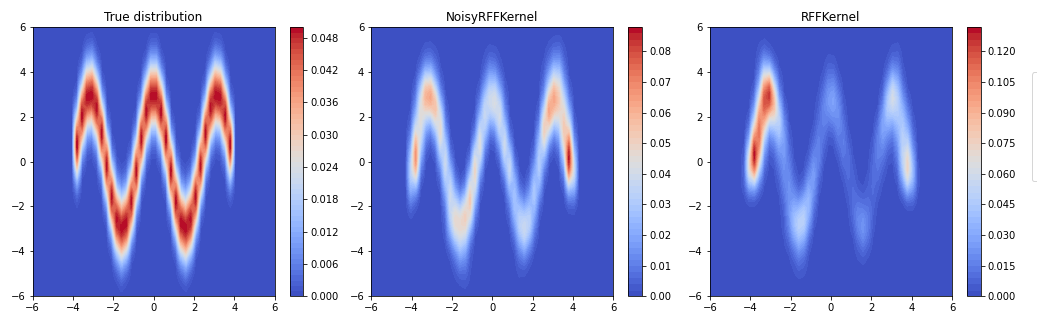
\includegraphics[width=\textwidth]{figures/score_matching/2D/Cosine3500.png}
%       \caption{Cosine}
%     \end{subfigure}

%     \begin{subfigure}[b]{\textwidth}
%       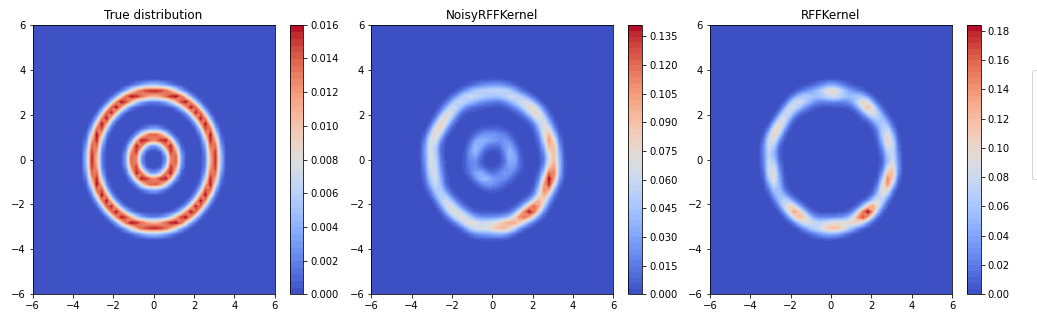
\includegraphics[width=\textwidth]{figures/score_matching/2D/Rings3500.png}
%       \caption{Mixture of rings}
%     \end{subfigure}

%     \caption{Score-matching density estimation using $3500$ sample size for cosine and the mixture of rings deistributions}
%     \label{fig:2d_3500}
% \end{figure}

\begin{figure}[H]
    \centering
    \begin{subfigure}[b]{0.32\textwidth}
        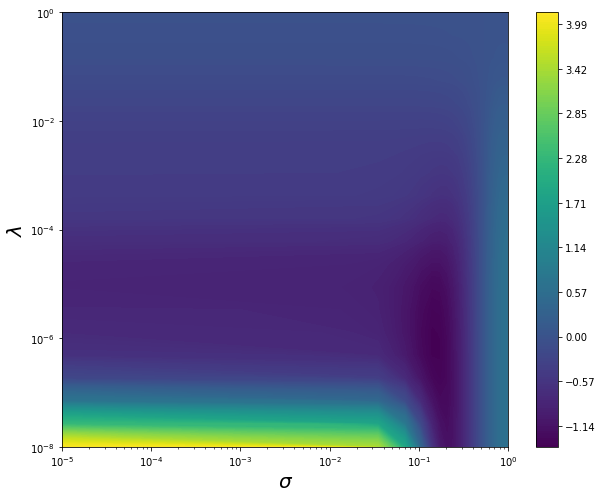
\includegraphics[width=\textwidth]{figures/score_matching/loss/lossCosine.png}
        \caption{Cosine}
    \end{subfigure}
    \begin{subfigure}[b]{0.32\textwidth}
        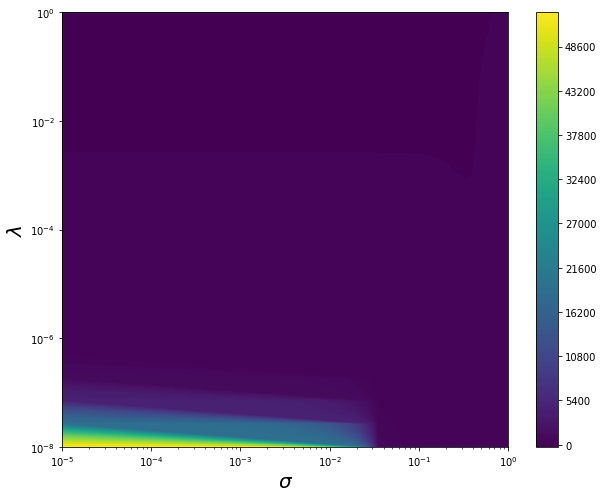
\includegraphics[width=\textwidth]{figures/score_matching/loss/lossBanana.png}
        \caption{Banana}
    \end{subfigure}
    \begin{subfigure}[b]{0.32\textwidth}
        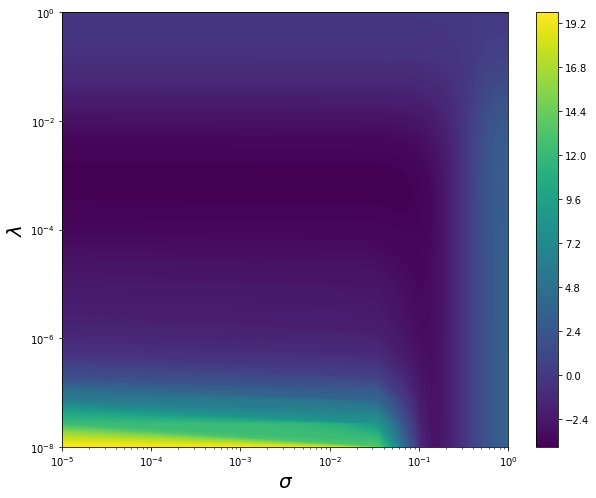
\includegraphics[width=\textwidth]{figures/score_matching/loss/lossRing.png}
        \caption{Ring}
    \end{subfigure}
  \begin{subfigure}[b]{0.32\textwidth}
    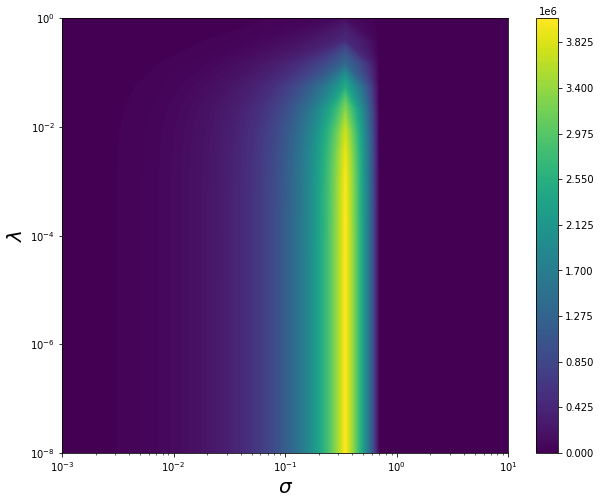
\includegraphics[width=\textwidth]{figures/score_matching/loss/lossMinibone.png}
    \caption{MiniBoone}
  \end{subfigure}
    \begin{subfigure}[b]{0.32\textwidth}
        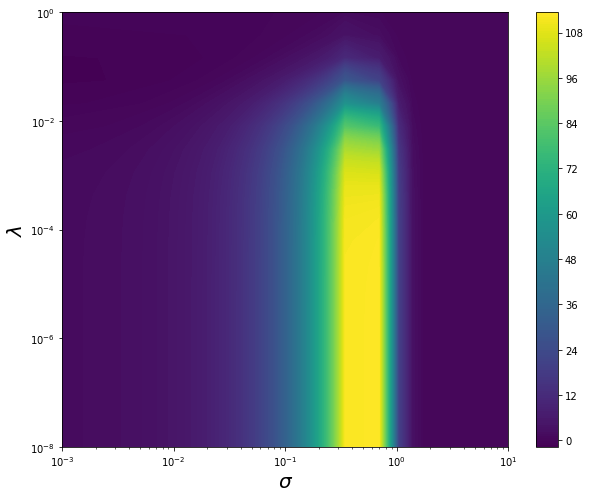
\includegraphics[width=\textwidth]{figures/score_matching/loss/lossRedWine.png}
        \caption{Red Wine}
    \end{subfigure}
    \begin{subfigure}[b]{0.32\textwidth}
        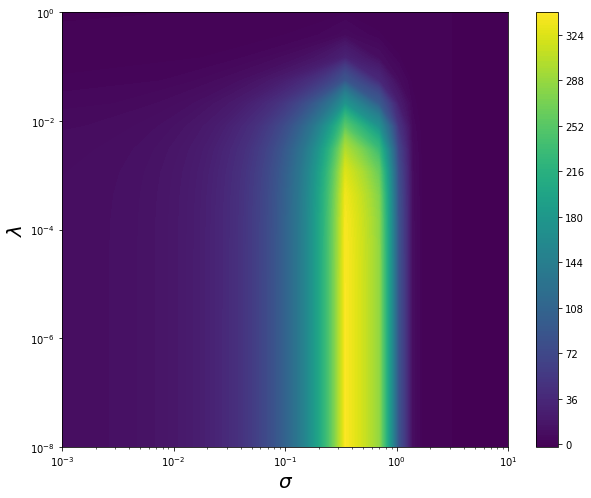
\includegraphics[width=\textwidth]{figures/score_matching/loss/lossWhiteWine.png}
        \caption{White Wine}
    \end{subfigure}
    \caption{Loss surface w.r.t. regularization parameter $\lambda$ (y axis) and noise parameter $\sigma$ (x axis).}
    \label{fig:lossdemo_app}
\end{figure}

\begin{figure}[H]
    \centering
    \begin{subfigure}[b]{0.8\textwidth}
        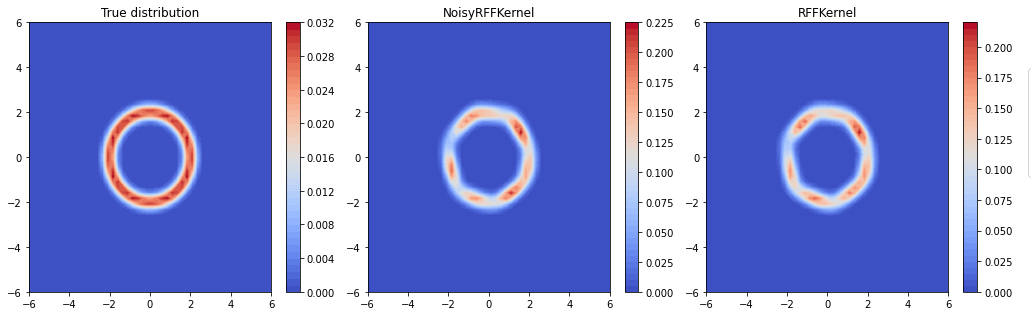
\includegraphics[width=\textwidth]{figures/score_matching/2D/ring1000MOG.png}
        \caption{Ring}
    \end{subfigure}

    \begin{subfigure}[b]{0.8\textwidth}
        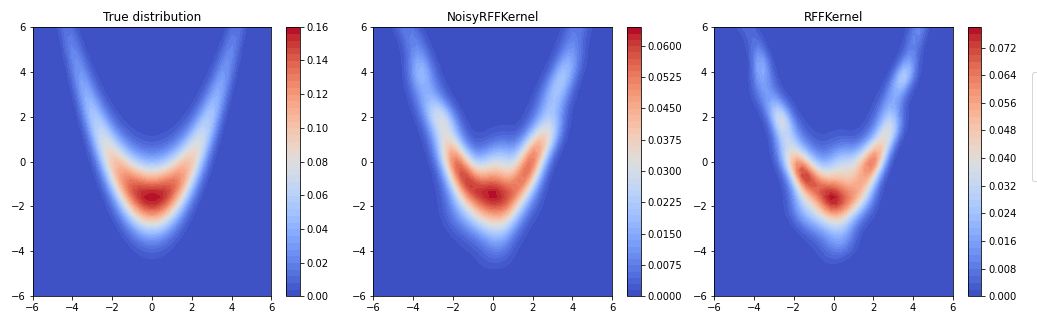
\includegraphics[width=\textwidth]{figures/score_matching/2D/Banana1000.png}
        \caption{Banana}
    \end{subfigure}

    \begin{subfigure}[b]{0.8\textwidth}
        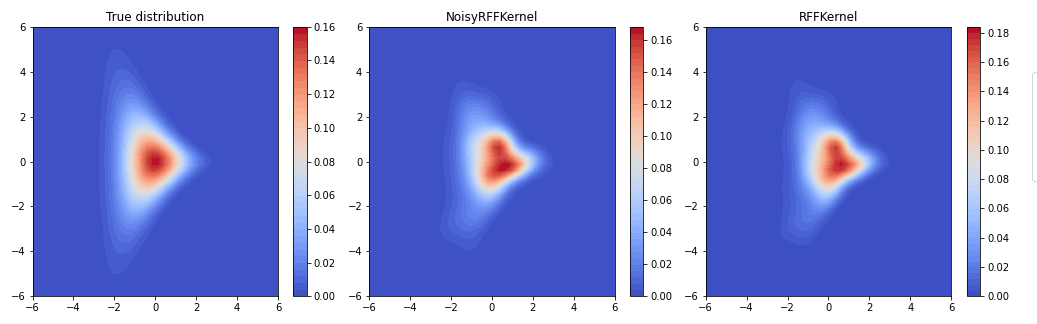
\includegraphics[width=\textwidth]{figures/score_matching/2D/Funnel1000.png}
        \caption{Funnel}
    \end{subfigure}

    \begin{subfigure}[b]{0.8\textwidth}
        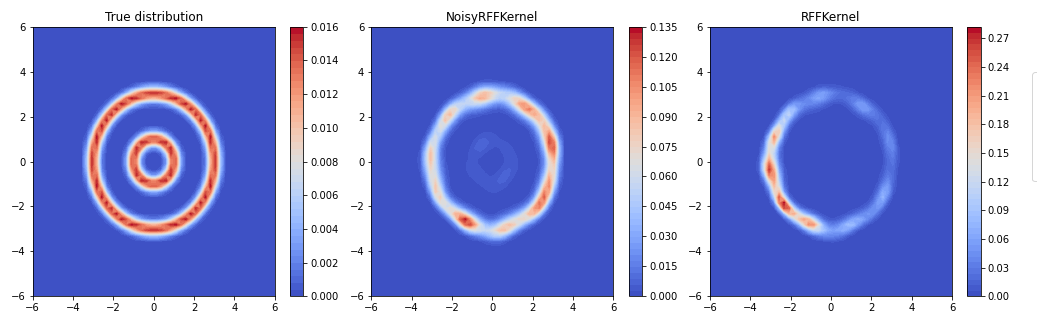
\includegraphics[width=\textwidth]{figures/score_matching/2D/Rings1000.png}
        \caption{Mixture of rings}
    \end{subfigure}

    \begin{subfigure}[b]{0.8\textwidth}
        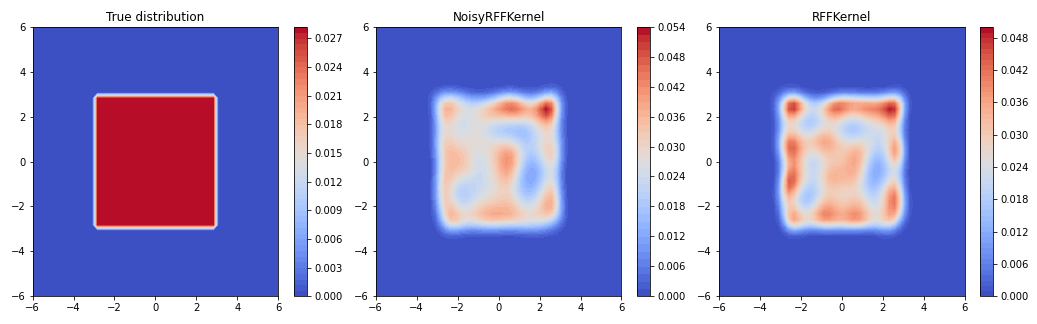
\includegraphics[width=\textwidth]{figures/score_matching/2D/Uniform1000.png}
        \caption{Uniform}
    \end{subfigure}

    \caption{Score-matching density estimation using $1000$ samples.
    Left column is a ground truth, middle is DSM RFf,
    right~--- SM RFF.}
    \label{fig:2d_1000_app}
\end{figure}


\addtocontents{toc}{\vspace{2em}}  % Add a gap in the Contents, for aesthetics
\backmatter

%% ----------------------------------------------------------------
\label{Bibliography}
\lhead{\emph{Bibliography}}  % Change the left side page header to "Bibliography"
\bibliographystyle{icml2020}  % Use the "unsrtnat" BibTeX style for formatting the Bibliography
\bibliography{Bibliography}  % The references (bibliography) information are stored in the file named "Bibliography.bib"

\end{document}  % The End
%% ----------------------------------------------------------------
